% =====================================================================
% main.tex — VDA-rebuild manuscript
%
% Mission: pursue the original question "when does value-directed
% attention matter?" with a more accurate mathematical description than
% Herman Lab 2026-04-09 ("When Does Value-Directed Attention Matter?
% A Normative Model with Independent Attentional Benefit and Cost",
% Critique/source/main.pdf, READ-ONLY).
%
% Structural convention (mission §6.3): main.tex is a thin skeleton
% that \input{}s per-section files in sections/. Each rebuild
% increment touches one section file. Figures live in figures/ and
% are copied from sims/*/output/ by the increment that depends on
% them. Bibliography in refs.bib.
%
% Per CLAIM_LEDGER.md, no manuscript claim may exceed the rebuilt
% strength licensed by the live verdict ledger
% (Critique/verdicts/). Distributional / conditional / graded voice
% by default; categorical floors and "regardless" statements are
% the exact failure the rebuild exists to fix (mission §3.3).
%
% Build: see BUILD.md. Tooling is plain pdflatex (latexmk not in
% sandbox); run twice for refs/cross-refs.
% =====================================================================

\documentclass[11pt]{article}

% --- packages ---
\usepackage[utf8]{inputenc}
\usepackage[T1]{fontenc}
\usepackage{lmodern}
\usepackage[a4paper, margin=1in]{geometry}
\usepackage{amsmath, amssymb, amsthm}
\usepackage{mathtools}
\usepackage{graphicx}
\usepackage{booktabs}
\usepackage{xcolor}
\usepackage[colorlinks=true, allcolors=blue!50!black]{hyperref}
% cleveref is not in TeX Live 2026basic; plain \ref{...} used in
% section files instead (e.g. "Section~\ref{sec:model}").

% --- theorem environments ---
\newtheorem{theorem}{Theorem}
\newtheorem{proposition}[theorem]{Proposition}
\newtheorem{lemma}[theorem]{Lemma}
\newtheorem{corollary}[theorem]{Corollary}
\theoremstyle{definition}
\newtheorem{definition}{Definition}
\newtheorem{assumption}{Assumption}
\theoremstyle{remark}
\newtheorem{remark}{Remark}

% --- shorthand notation aligned with Critique/source/main.pdf §2 ---
\newcommand{\Phinorm}{\Phi}                 % standard normal CDF
\newcommand{\HR}{\mathrm{HR}}               % hit rate
\newcommand{\FAR}{\mathrm{FAR}}             % false alarm rate
\newcommand{\dprime}{d'}                    % discriminability
\newcommand{\dprimemax}{d'_{\max}}
\newcommand{\Nloc}{N}                       % number of locations
\newcommand{\val}{v}                        % cued value
\newcommand{\valid}{V}                      % cued validity
\newcommand{\alphacued}{\alpha_c}           % cued attention
\newcommand{\alphauncued}{\alpha_u}         % uncued attention
\newcommand{\benefit}{\beta}                % attention benefit weight
\newcommand{\cost}{\gamma}                  % attention cost weight
\newcommand{\Rew}{R}                        % expected reward
\newcommand{\Rpone}{R_{\mathrm{P1}}}        % policy P1 expected reward
\newcommand{\Rptwo}{R_{\mathrm{P2}}}
\newcommand{\Rpthree}{R_{\mathrm{P3}}}
\newcommand{\Rpfour}{R_{\mathrm{P4}}}
\newcommand{\VDA}{\mathrm{VDA}}
\newcommand{\CF}{\mathrm{CF}}               % criterion fraction
\newcommand{\corr}{\rho}                    % cross-location correlation (A1 channel)
\newcommand{\PnoFA}{P_{\mathrm{no\text{-}fa}}}
\newcommand{\Rsens}{r}                      % benefit/cost ratio (A3)
\newcommand{\rdagger}{r^{\dagger}}          % VDA-escape threshold (C2)
\newcommand{\rstarinv}{r^{*}_{\mathrm{inv}}}% inversion threshold (C4)
\newcommand{\CR}{\mathrm{CR}}               % conservation rule indicator
\newcommand{\DKL}{D_{\mathrm{KL}}}           % Kullback--Leibler divergence (A3 derivation)

% --- metadata ---
\title{When does value-directed attention matter?\\[2pt]
       \large A three-lever normative model with quantified
       criterion, sensitivity, and decorrelation contributions
       (rebuild draft, v0.1)}
\author{[Authors -- TBD]\thanks{Rebuild of the Herman Lab
        2026-04-09 manuscript with the same scientific question and
        a more honestly-bounded mathematical description. See
        \texttt{CLAIM\_LEDGER.md} for the disposition table that
        binds every claim to its supporting artifact.}}
\date{Draft compiled \today}

\begin{document}
\maketitle

% =====================================================================
% Section files. Each section file is a stub at rb-005 and gets filled
% by a later increment (RB-009 -> results-C1, RB-010 -> results-C2,
% RB-011 -> §5.2 redrafted design advice, RB-012 -> results-C4,
% RB-013 -> appendix-C5, RB-004 -> model, ...). See REBUILD_BACKLOG.md.
% =====================================================================

% =====================================================================
% abstract.tex — DRAFTED at rb-047 (RB-047), 2026-05-30.
%
% Filled after the body of the manuscript landed:
%   - sec:model (rb-009, RB-004), three-lever reframe.
%   - sec:results-c1..c4 (rb-006, rb-007, rb-011, rb-013).
%   - sec:extensions-A3, A2, A8 (rb-017, rb-022, rb-028).
%   - sec:appendix-c5 (rb-018), sec:appendix-deriv-c2 (rb-024),
%     sec:appendix-deriv-a3 (rb-046).
%
% Strength check (mission §3, CLAIM_LEDGER.md): every quantitative
% claim below is at the licensed band / distributional / conditional
% strength.  Original-paper categorical phrasings (CF floor [0.60,
% 0.96]; "negligible regardless of other parameters"; uniform
% no-inversion; A1 upper bound on VDA) appear here only as the thing
% being retracted, not stated.
% =====================================================================

\begin{abstract}
\noindent
In a cued change-detection task whose cue carries both value
$\val \ge 1$ and validity $\valid \in [1/\Nloc, 1]$, an ideal observer
can adapt to value by shifting decision criteria, by re-allocating
spatial attention, or, when noise is correlated across locations, by
\emph{decorrelating} the encoded population code.  We rebuild the
normative model of \emph{value-directed attention} (VDA) around this
three-lever decomposition (Section~\ref{sec:model},
Definition~\ref{def:three-levers}), with cross-location correlation
$\corr$ promoted to a first-class model parameter via an exact
one-factor Gauss--Hermite reduction that recovers the inherited
independent-noise model in the limit $\corr \to 0$ to floating-point
identity.  The rebuilt manuscript reports every headline result at
its defensible distributional, graded, or conditional strength
rather than as a categorical floor.

Across a $4{,}410$-cell sweep over $(\valid, \val, \Rsens)$, the
criterion fraction $\CF$ is concentrated in $[0.30, 1.00]$ with
median $0.76$; the published $[0.60, 0.96]$ interval is retracted on
both ends, and adding $\corr = 0.2$ drops the strict minimum below
$0.5$ (Section~\ref{sec:results-c1}).  $\VDA$ is non-monotonic in
$\Rsens$ as in the inherited paper; we strengthen this result with
the closed-form escape threshold
$\rdagger(\val) = K_u(\val) / [(\Nloc - 1) K_c(\val)]$ that pins the
lower edge of the VDA-active band (Section~\ref{sec:results-c2}),
extend it to $\corr > 0$ via the natural $\corr$-aware gradient
quadratures (Appendix~\ref{sec:appendix-deriv-c2}), and prove that
$\rdagger(\val)$ is invariant under the conservation order of the
benefit/cost rule (Appendix~\ref{sec:appendix-deriv-a3}).  The
``narrow regime'' for VDA becomes a quantitative iso-$\VDA$ contour
band (Section~\ref{sec:results-c3}): at $\valid \ge 0.95$ peak
$\VDA$ sits at the grid floor under any $(\Rsens, \corr)$; at
$\valid \ge 0.80$ this survives only at $\corr = 0$; at
$\valid \ge 0.60$ it fails.  The ``no inversion'' result is restated
as a conditional theorem with the explicit condition
$\valid \ge 1 / [(\Nloc - 1) \val + 1]$, and the rebuild adds the
\emph{anti-cue inversion} as a new falsifiable prediction
(Section~\ref{sec:results-c4}, Equation~\eqref{eq:value-weight}):
under counter-predictive cues ($\valid < 1/\Nloc$) at $\Nloc = 4$,
the globally optimal allocation places \emph{less} attention at the
high-value location in $36.1\%$ of probed cells.  Symmetric recovery
at $\Rsens = 1$ is reaffirmed as a universal real-number identity
(Appendix~\ref{sec:appendix-c5}, conservation-form-invariant by
construction).

Independence is not an upper bound on $\VDA$.  What independence
actually upper-bounds is the criterion fraction, and only in
variant~A: $\partial \VDA / \partial \corr$ flips sign near
$\Rsens \approx 0.5$, with the cell-wise crossover sweeping past
$\Rsens \approx 0.79$ across the full sweep
(Section~\ref{sec:model-upper-bound}).  Within-display heterogeneity
of $\Rsens$ is a bounded perturbation that leaves the $C_2$ peak
coordinates and the contested-CF corner essentially invariant
(Section~\ref{sec:extensions-a2}); the additive
$\benefit + \cost = 2$ rule is one point in the power-mean
conservation family, and the headline numbers are reported as a
band over that family (Section~\ref{sec:extensions-a3}); the
homogeneous-uncued result is innocuous at the inherited additive
optimum but can fail in a benefit-dominant symmetric-stress corner
when the conservation rule is multiplicative
(Section~\ref{sec:extensions-a8}).  Every quantitative claim above
is backed by a simulation under \texttt{Rebuild/sims/} with a
recovered limit, a deterministic output hash, and a captioned
figure; every novel proposition is derived under
\texttt{Rebuild/derivations/}; nothing in this abstract is stated
more strongly than its row of \texttt{CLAIM\_LEDGER.md} licenses.
\end{abstract}

% =====================================================================
% intro.tex — DRAFTED at rb-049 (RB-049), 2026-05-30.
%
% Third bookend; companion of sections/abstract.tex (rb-047, RB-047)
% and sections/limitations.tex (rb-048, RB-048).  Mirrors the abstract's
% voice (distributional / graded / conditional by default) and sets up
% the §3.3 unifying-reframe contrast that the §limitations §7.6 'what
% the rebuild does not claim' paragraph closes on.
%
% Strength check (mission §3, CLAIM_LEDGER.md): every quantitative
% claim below is at the licensed band / distributional / conditional
% strength already wired in the body sections.  Original-paper
% categorical phrasings (CF floor [0.60, 0.96]; "negligible regardless
% of other parameters"; uniform no-inversion; A1 upper bound on VDA)
% appear here only as the framing being retracted, not stated.
% =====================================================================

\section{Introduction}
\label{sec:intro}

In a cued change-detection task whose cue carries both \emph{value}
$\val \ge 1$ and \emph{validity} $\valid \in [1/\Nloc, 1]$, an
observer adapting to the value contingency has more than one lever
available.  They may shift decision criteria so that responses at the
high-value location are biased toward report; they may re-allocate
spatial attention so that the perceptual evidence at the high-value
location is itself more reliable; and, when noise is correlated
across locations, they may decorrelate the encoded population code so
that the joint evidence drawn from the unattended array is less
redundant.  The original \emph{value-directed attention} (VDA) model
asks a sharp normative question on top of these levers: how much of
the behavioural adaptation to value is achieved by re-allocating
attention toward the high-value location versus by shifting decision
criteria, and in what parameter regime does attention re-allocation
become the dominant mechanism?  This paper preserves that question
verbatim in spirit.  What changes is the mathematical description used
to answer it.

The inherited model couples value-driven sensitivity changes to a
single attentional asymmetry parameter and decomposes the expected
reward across nested policies that toggle each lever on or off.  Its
quantitative claims, however, tend to overstate what their underlying
simulations license: a central or peak value is repeatedly reported
as a uniform floor, a directional inequality, or a
``regardless of other parameters'' constant.  Re-evaluating those
claims against the model's own definitions reveals a recurring
mismatch.  The reported criterion-fraction interval $[0.60, 0.96]$ is
in fact $[0.30, 1.00]$ across the same $4{,}410$-cell sweep with
median $0.76$ and a $\sim\!13\%$ tail below $0.60$; the
``high-validity paradigms show negligible VDA regardless of other
parameters'' design recommendation holds at $\valid \ge 0.95$ but
not at $\valid \approx 0.80$ once cross-location correlation is
admitted; the ``no inversion'' result is true everywhere in the cued
regime but not in the anti-cue regime $\valid < 1/\Nloc$; and the
self-characterisation of independence as ``an upper bound on VDA'' is
sign-ambiguous --- correlation \emph{suppresses} VDA in the
cost-dominant regime and \emph{amplifies} it in the
benefit-dominant tail.  None of these reframings overturns the
underlying mechanism the original paper identified.  Each one
restates a central tendency, a graded boundary, or a conditional
theorem in place of an unconditional one.  Reporting distributions,
quantiles, contour bands, and explicit conditions \emph{instead of}
floors, ``never,'' and ``regardless of'' is the corrective this paper
applies uniformly: distributional, graded, or conditional by default.

Restating the model in this voice also exposes a missing lever.  The
inherited two-channel decomposition treats criterion shifts and
sensitivity re-allocation as the only adaptive mechanisms; the
empirically dominant decorrelation channel
\cite{CohenMaunsell2009,
RuffCohen2016,
Srinath2021} is excluded by an
independence assumption that the model bundles into its
no-false-alarm probability.  Section~\ref{sec:model} promotes
cross-location correlation $\corr$ to a first-class model parameter
through an exact one-factor Gauss--Hermite reduction of the
equicorrelated-Gaussian orthant integral, recovering the inherited
independent-noise model in the limit $\corr \to 0$ to floating-point
identity (Equation~\eqref{eq:pnofa-rho},
Equation~\eqref{eq:rho-zero-recovery}).  This yields the rebuilt
paper's central reframe: three levers, not two
(Definition~\ref{def:three-levers}; criterion shift,
sensitivity re-allocation, decorrelation).  The inherited model's
self-characterisation of independence as an upper bound on VDA is
replaced by a more careful statement: what independence actually
upper-bounds is the criterion fraction $\CF$ ---
$\CF(\corr) \le \CF(0)$ pointwise in variant~A by a Slepian
monotonicity argument (Appendix~\ref{sec:appendix-deriv-a1}) --- while
$\partial \VDA / \partial \corr$ flips sign near $\Rsens \approx 0.5$
at the headline cell and sweeps a cell-wise crossover up to
$\Rsens \approx 0.79$ across the full $4{,}410$-cell sweep
(Section~\ref{sec:model-upper-bound},
Table~\ref{tab:a1cw-summary}).

Under the corrective voice, the four headline C-row results recover
in distributional, graded, and conditional forms.  The criterion
fraction is concentrated in $[0.30, 1.00]$ with median $0.76$
(Section~\ref{sec:results-c1}, Table~\ref{tab:cf-distribution});
$\VDA$ is non-monotonic in $\Rsens$ with a closed-form lower edge
$\rdagger(\val) = K_u(\val) / [(\Nloc - 1) K_c(\val)]$
(Equation~\eqref{eq:r-dagger}) that extends to $\corr > 0$ through
$\corr$-aware gradient quadratures
(Section~\ref{sec:appendix-deriv-c2},
Proposition~\ref{prop:r-dagger-rho}) and is invariant under the
benefit/cost conservation order
(Proposition~\ref{prop:r-dagger-invariance}); the ``narrow regime''
becomes a quantitative iso-$\VDA$ contour band
(Section~\ref{sec:results-c3}, Table~\ref{tab:c3-highV-probe}) with
hierarchical $\valid$ thresholds ($\valid \ge 0.95$ at the grid floor
under any $(\Rsens, \corr)$; $\valid \ge 0.80$ only at $\corr = 0$;
$\valid \ge 0.60$ fails); and the no-inversion result becomes a
conditional theorem with the explicit boundary
$\valid \ge 1 / [(\Nloc - 1) \val + 1]$
(Section~\ref{sec:results-c4}, Equation~\eqref{eq:value-weight})
that, when crossed, generates a new falsifiable prediction --- the
\emph{anti-cue inversion}: under counter-predictive cues
($\valid < 1/\Nloc$) at $\Nloc = 4$, the normatively optimal
allocation places \emph{less} attention at the high-value location
in $36.1\%$ of probed cells (Table~\ref{tab:c4-anticue}).  Symmetric
recovery at $\Rsens = 1$ is reaffirmed as a universal real-number
identity (Appendix~\ref{sec:appendix-c5},
Proposition~\ref{prop:c5-realnumber}), conservation-form-invariant by
construction (Corollary~\ref{cor:a3d-c5-invariance}).

Three further mechanisms the inherited model held fixed at
homogeneous values return as explicit extensions.
Within-display heterogeneity of $\Rsens$ is a bounded perturbation
that leaves the $C_2$ peak coordinates and the contested-CF corner
essentially invariant (Section~\ref{sec:extensions-a2},
Table~\ref{tab:a2-rb021-summary}).  The benefit/cost conservation
rule $\benefit + \cost = 2$ is one point in the power-mean
conservation family
(Equation~\eqref{eq:conservation-family},
Equation~\eqref{eq:beta-gamma-of-p}); the rebuilt paper reports
every headline number as a band over the family at
$p \in \{0, 0.5, 1\}$ with the per-cell monotonicity
$\Delta \CF(\corr = 0) \le 0$ stated as
Theorem~\ref{thm:delta-cf-monotone}
(Section~\ref{sec:extensions-a3}).  The $N$-dimensional uncued
allocation policy is innocuous at the inherited additive optimum but
exhibits a new conditional binding in a benefit-dominant
symmetric-stress corner under multiplicative conservation, with a
$32\%$ $\corr$-amplification at the focal cell
(Section~\ref{sec:extensions-a8}).  Per-location decision-noise
coupling --- a candidate fourth lever
--- is named and held at the live status of its underlying claim
(Section~\ref{sec:limitations-a6}) rather than wired into the model.

The remainder of the manuscript follows this layout.
Section~\ref{sec:model} states the rebuilt model with the
three-lever decomposition and the $\corr$-channel reduction.
Section~\ref{sec:results} reports the C-row headline results in the
distributional / graded / conditional voice, with each subsection
naming the inherited categorical claim it replaces.
Section~\ref{sec:extensions} runs the three lever extensions
(A2, A3, A8) at empirical band strength.
Section~\ref{sec:limitations} catalogues the explicit scope of
every claim --- in particular, what the rebuilt model does
\emph{not} claim about neural implementation,
empirical-$\corr$ prediction, observer-deviation, or attention
dynamics.  The appendix collects the formal derivations
(A1 $\corr$ channel, $C_2$ closed forms,
$C_5$ symmetric recovery, A3 power-mean conservation).
Every quantitative claim in the body is backed by a simulation in
\texttt{Rebuild/sims/} with a recovered limit, a deterministic
output hash, and a captioned figure; every novel proposition is
derived in \texttt{Rebuild/derivations/}.  Reproducibility is
end-to-end byte-identical, and nothing in this paper is stated more
strongly than its row of \texttt{CLAIM\_LEDGER.md} licenses.

% =====================================================================
% model.tex — FILLED by rb-009 (RB-004).
%
% Discharges RB-004: the §model section of the rebuilt manuscript.
% Cites:
%   * Rebuild/derivations/A1--rho-channel.md (rb-008, RB-003) — the
%     full derivation that this section compresses into a main-text
%     statement.
%   * Rebuild/sims/A1--rho-channel/ (rb-002, RB-002, sha256
%     b692c06456530ccd1b319762d8a948814324d3129f39902ce9531a66d1206614)
%     — the backing simulation at the headline cell; figures
%     vda_curves_variantA.png, vda_curves_variantB.png, cf_vs_rho.png
%     copied into manuscript/figures/.
%   * Rebuild/model/tests/test_recovery.py (rb-001, sha256
%     d3c62215cedbe2f797c484a8d76e8bef1d5ac42cdb3092ff099a34aea1b6f18f)
%     — the ρ→0 recovery contract that pins the extended model to
%     the inherited model to floating-point identity.
%   * Rebuild/sims/C1--cf-distribution/ (rb-003, sha256
%     91fc4692dbc106eca9c90770c79e22f7f4757d76421ed55e7e8e91f80e44706c)
%     — for the cell-wise generalisation of the variant-A CF
%     upper-bound beyond the single headline cell.
%
% Allowed-strength ceiling (CLAIM_LEDGER.md A1 row, rb-008 reconcile):
%   * Three levers, not two: criterion + sensitivity + decorrelation.
%   * §5.5 "upper bound on VDA" of the inherited paper RETRACTED.
%     What independence actually upper-bounds is the criterion fraction
%     (variant A monotone-down in ρ at the headline cell and in 84%
%     of variant-A cells across the sweep; variant B essentially flat
%     at the headline cell and only 64% one-sided across the sweep —
%     reported as a sensitivity, not a uniform claim).
%   * Sign-flip of dVDA/dρ in r in the band [0.38, 0.56] at the
%     headline cell is a reported finding; the §4.3 of the derivation
%     names it Statement B, restricted to the empirical envelope.
% =====================================================================

\section{Model}
\label{sec:model}

The rebuilt model retains the inherited paper's signal-detection-
theoretic decomposition of the cued change-detection task and its
four nested policies; what it adds is a third lever — cross-location
noise correlation $\corr$ — that the inherited model omits by
assumption. This section states the inherited skeleton in compact
form (Section~\ref{sec:model-inherited}), localises the per-location
independence assumption A1 to the single algebraic place in the
expected-reward expression where it enters
(Section~\ref{sec:model-booking}), promotes that place to a tunable
parameter $\corr \in [0, 1)$ with an exact one-dimensional reduction
and a $\corr \to 0$ recovery contract that pins the extended model
to the inherited model at floating-point identity
(Section~\ref{sec:model-rho-channel}), and recasts the original
two-lever (criterion vs.\ sensitivity) decomposition as a three-lever
(criterion vs.\ sensitivity vs.\ decorrelation) decomposition
(Section~\ref{sec:model-three-levers}). The
section closes with a quantitative restatement of what an
independent-noise model is in fact an upper bound on
(Section~\ref{sec:model-upper-bound}): not VDA, but the criterion
fraction $\CF$, and even then in a variant- and cell-conditional
sense that the rebuilt manuscript reports as a distribution rather
than as a uniform inequality. The full derivation is in
Appendix~\ref{sec:appendix-deriv-a1}.

% ---------------------------------------------------------------------
\subsection{The inherited skeleton}
\label{sec:model-inherited}

Fix $\Nloc \ge 2$ locations, indexed so that $i = c$ is the cued
location and $i = 1, \dots, \Nloc-1$ enumerates the $\Nloc - 1$
uncued locations. Each location carries an equal-variance Gaussian
decision variable; under the per-location signal-detection model the
hit rate and false-alarm rate at $i$ are
\begin{equation}
  \HR_i \;=\; \Phinorm(\dprime_i/2 - c_i),
  \qquad
  \FAR_i \;=\; \Phinorm(-\dprime_i/2 - c_i),
  \label{eq:sdt-marginal}
\end{equation}
where $\dprime_i$ is sensitivity at $i$, $c_i$ is the decision
criterion at $i$, and $\Phinorm$ is the standard-normal cumulative
distribution function. The attention map
$\alphacued + (\Nloc - 1)\,\alphauncued = 1$ assigns a continuous
share of attention to each location, and an asymmetric transfer
$\dprime_c = \dprimemax \cdot f(\alphacued;\, \benefit(\Rsens))$,
$\dprime_u = \dprimemax \cdot f(\alphauncued;\, \cost(\Rsens))$
maps allocation to sensitivity through a benefit weight
$\benefit(\Rsens)$ and a cost weight $\cost(\Rsens)$. The
benefit/cost ratio $\Rsens$ is a single scalar that controls the
relative magnitude of an attentional gain at the focus and an
attentional loss at the periphery; under the inherited (variant-A)
\emph{additive conservation rule}
$\benefit(\Rsens) + \cost(\Rsens) = 2$, with
$\benefit(\Rsens) = 2\Rsens/(\Rsens + 1)$ and
$\cost(\Rsens) = 2/(\Rsens + 1)$. The two reward variants used
throughout the manuscript are variant~A (value-scaled correct
rejections, $\CR = \valid \val + (1 - \valid)$) and variant~B
($\CR = 1$); the additive conservation rule is varied in
Section~\ref{sec:limitations} (assumption A3, RB-015/RB-019). The
notation matches \texttt{Rebuild/model/core.py}: see
\texttt{d\_prime\_asym}, \texttt{beta\_gamma}, \texttt{floor\_R}, and
\texttt{policies} for the validated reference implementation.

The expected reward over change and no-change trials is
\begin{equation}
  \mathbb{E}[\Rew]
  \;=\;
  \tfrac{1}{2}\big[\,\valid\,\HR_c\,\val
                  \,+\,(1-\valid)\,\HR_u\,\big]
  \;+\;
  \tfrac{1}{2}\,\PnoFA\,\CR,
  \label{eq:expected-reward}
\end{equation}
where $\PnoFA = \Pr(\text{no location false-alarms on a no-change
trial})$ is the only term in (\ref{eq:expected-reward}) that involves
more than one location at a time. Four nested policies P1--P4
optimise (\ref{eq:expected-reward}) over progressively shrinking
parameter sets: P1 jointly optimises $(\alphacued, c_c, c_u)$ at the
operating value $\val$; P2 freezes $\alphacued$ at the
$\val = 1$ optimum and re-optimises only the criteria; P3 holds the
criteria at the P4 floor and re-optimises only $\alphacued$; P4 holds
both $\alphacued$ and the criteria at their $\val = 1$ floors. The
value-directed-attention benefit is the gain in reward from
re-allocating attention with both criteria already adapted,
\begin{equation}
  \VDA \;:=\; \Rpone - \Rptwo,
  \label{eq:vda-def}
\end{equation}
and the criterion fraction is the share of the value-related reward
gain that criterion shifts alone capture,
\begin{equation}
  \CF \;:=\;
  \frac{\Rpthree - \Rpfour}{\Rpone - \Rpfour}.
  \label{eq:cf-def-model}
\end{equation}
Equation~(\ref{eq:cf-def-model}) is the metric the inherited paper's
§5.1 stated had a floor at $0.60$; we report its true range and
distribution in Section~\ref{sec:results-c1}.

% ---------------------------------------------------------------------
\subsection{The locus of assumption~A1}
\label{sec:model-booking}

Assumption~A1 of the inherited paper is per-location independence of
the decision variables. We are now in a position to read off exactly
where this assumption enters (\ref{eq:expected-reward}). The change-
trial bracket of (\ref{eq:expected-reward}) is linear in the marginal
hit rates $\HR_c, \HR_u$: on a change trial the change happens at a
single location (cued with probability $\valid$, a specific uncued
with probability $(1 - \valid)/(\Nloc - 1)$), so no product of
probabilities across locations appears. The only cross-location
product is in the no-change-trial bracket, through $\PnoFA$. Under
independence,
\begin{equation}
  \PnoFA^{\text{indep}}
  \;=\;
  \prod_{i} (1 - \FAR_i)
  \;=\;
  \Phinorm(b_c)\,\Phinorm(b_u)^{\Nloc - 1},
  \qquad
  b_i := c_i + \dprime_i/2,
  \label{eq:pnofa-indep}
\end{equation}
where $b_i \in \mathbb{R}$ is the $z$-score the no-change decision
variable must stay below. Equation~(\ref{eq:pnofa-indep}) is the
sole appearance of A1 in (\ref{eq:expected-reward}); the faithful
and complete relaxation of A1 within the reward structure is
therefore the replacement of this product by the correlated joint
orthant probability.

\begin{remark}
The booking here matters because it isolates A1 from a distinct
relaxation that the inherited paper's §5.5 sometimes conflates with
correlated noise: a global ``change-detected-somewhere'' decision
rule. The latter would replace the per-location decision statistics
with a pooled detection statistic and is a relaxation of A6
(homogeneous decision rule), not of A1. A1 is exactly
(\ref{eq:pnofa-indep}); see
Appendix~\ref{sec:appendix-deriv-a1}, §1.2 for the formal version
of the same booking.
\end{remark}

% ---------------------------------------------------------------------
\subsection{The decorrelation channel}
\label{sec:model-rho-channel}

We promote the per-location-independence assumption to a tunable
equicorrelation parameter $\corr \in [0, 1)$. Let the no-change
decision variables be jointly Gaussian with standardised marginals
and equicorrelation,
\begin{equation}
  \mathbf{X} \;\sim\; \mathcal{N}(\boldsymbol\mu, \Sigma),
  \qquad
  \mu_i = -\dprime_i/2,
  \qquad
  \Sigma_{ii} = 1,
  \qquad
  \Sigma_{ij} = \corr \ (i \neq j).
  \label{eq:equicorr-cov}
\end{equation}
The one-factor representation
$X_i = \mu_i + \sqrt{\corr}\,Z + \sqrt{1 - \corr}\,\varepsilon_i$
(with $Z, \varepsilon_1, \dots, \varepsilon_\Nloc$ i.i.d.\
$\mathcal{N}(0, 1)$) reproduces (\ref{eq:equicorr-cov}) and makes the
$X_i$ conditionally independent given $Z$. Multiplying the
conditional event probabilities, then integrating out $Z$ against the
standard-normal density $\varphi$, yields the exact one-dimensional
integral
\begin{equation}
  \boxed{\;
    \PnoFA(\corr)
    \;=\;
    \int_{-\infty}^{\infty}
    \Phinorm\!\left(\frac{b_c - \sqrt{\corr}\,z}{\sqrt{1 - \corr}}\right)
    \Phinorm\!\left(\frac{b_u - \sqrt{\corr}\,z}{\sqrt{1 - \corr}}\right)^{\!\Nloc - 1}
    \varphi(z)\,dz.
  \;}
  \label{eq:pnofa-rho}
\end{equation}
Equation~(\ref{eq:pnofa-rho}) is exact for any $\Nloc$ and any
$\corr \in [0, 1)$. No multivariate-normal CDF is needed;
equicorrelation collapses the $\Nloc$-dimensional integral to a one-
dimensional one. The rebuilt model evaluates
(\ref{eq:pnofa-rho}) by 64-node Gauss--Hermite quadrature in
\texttt{Rebuild/model/core.py:p\_no\_fa\_point} and
\texttt{:p\_no\_fa\_grid}, with quadrature error $\le 10^{-15}$
against a 128-node reference across the operating
$\corr \in \{0, 0.05, 0.1, 0.2, 0.3, 0.4\}$ band.

At $\corr = 0$ the integrand of (\ref{eq:pnofa-rho}) is constant in
$z$ and the integral reduces to (\ref{eq:pnofa-indep}):
\begin{equation}
  \PnoFA(0) \;=\;
  \Phinorm(b_c)\,\Phinorm(b_u)^{\Nloc - 1}.
  \label{eq:rho-zero-recovery}
\end{equation}
Equation~(\ref{eq:rho-zero-recovery}) is the \emph{recovery contract}
the extended model is bound to honour, and the contract is enforced
in \texttt{Rebuild/model/tests/test\_recovery.py}: with $\corr$
clamped to zero, the extended-model headline VDA, CF, and
$\Rew_{\text{P}_k}$ values reproduce the inherited model's reference
numbers (sourced from
\texttt{Critique/replications/A1--correlated-fa/}) at floating-point
identity, including the peak
$\VDA^{\star}(\corr{=}0) = 0.07986$ at $\Rsens = 0.3831$
(sha256 \texttt{d3c62215\ldots}, 7/7 \textsc{pass}). The recovery
contract is global to the rebuilt manuscript: any subsequent model
extension that re-implements no-FA computation
(Section~\ref{sec:limitations}; the heterogeneous-$\Rsens$ extension
RB-014/RB-018, the conservation-family extension RB-015/RB-019) must
pass its own $\corr = 0$ limit before its new regime is admitted.

The empirical envelope of the rebuilt manuscript is
$\corr \in [0, 0.4]$, which brackets the $r_\mathrm{SC} \approx 0.2$
range reported in macaque V4 during peripheral-validity-cue change-
detection by Cohen and Maunsell~\cite{CohenMaunsell2009}; higher
$\corr$ values are admissible in the model but are not used to
anchor any headline claim. Equicorrelation is a deliberate one-
parameter simplification; structured covariances
\cite{RuffCohen2016, Srinath2021} break the exact 1-D reduction
(\ref{eq:pnofa-rho}) and are flagged as a scoped limitation in
Section~\ref{sec:limitations}. The full derivation of
(\ref{eq:pnofa-rho}), with the Slepian monotonicity inequality
$\PnoFA(\corr) \ge \PnoFA(0)$ \cite{Slepian1962} that it satisfies,
is in Appendix~\ref{sec:appendix-deriv-a1}.

% ---------------------------------------------------------------------
\subsection{Three levers, not two}
\label{sec:model-three-levers}

The inherited paper decomposes the value effect into two levers:
\emph{criterion shift} (P3 $\to$ P4) and \emph{sensitivity
re-allocation} (P1 $\to$ P3). With $\corr$ promoted to a model
parameter, the same expected-reward expression
(\ref{eq:expected-reward}) admits a third lever — \emph{decorrelation}
— that the inherited model cannot represent because it sits
permanently at $\corr = 0$.

\begin{definition}[The three levers]
\label{def:three-levers}
At fixed $(\Nloc, \valid, \val, \dprimemax, f_0, h, \CR, \Rsens)$, the
rebuilt model exposes three independent mechanisms by which an
observer can adapt to a non-trivial cue:
\begin{enumerate}
\item \textbf{Criterion shift} — moving $(c_c, c_u)$ off the
  $\val = 1$ floor. Its standalone reward contribution is
  $\Rpthree - \Rpfour$; its share of the value-related gain is
  $\CF$ (\ref{eq:cf-def-model}).
\item \textbf{Sensitivity re-allocation} — moving $\alphacued$ off
  the $\val = 1$ optimum. Its standalone reward contribution at
  adapted criteria is $\Rpone - \Rptwo = \VDA$
  (\ref{eq:vda-def}).
\item \textbf{Decorrelation} — moving $\corr$ off the inherited
  $\corr = 0$ corner. By Slepian monotonicity,
  $\PnoFA(\corr)$ is non-decreasing in $\corr$ at fixed
  $(b_c, b_u)$ \cite{Slepian1962}, which lifts every per-policy
  supremum reward $\Rew_{\text{P}_k}(\corr)$ above its
  $\corr = 0$ value (see Appendix~\ref{sec:appendix-deriv-a1},
  Corollary~3.2).
\end{enumerate}
\end{definition}

The decorrelation lever is not a free third mechanism the rebuild
adds; it is the lever the inherited paper implicitly held fixed at
the boundary of its admissible parameter space. Promoting $\corr$ to
a model parameter is the minimal extension that lets the
manuscript report what the rebuilt expected-reward expression
actually does as that parameter is varied.

% ---------------------------------------------------------------------
\subsection{What independence actually upper-bounds}
\label{sec:model-upper-bound}

The §5.5 sentence of the inherited paper states that the
independent-noise results ``therefore represent an upper bound on
VDA benefit.'' Once $\corr$ is a model parameter, this sentence
becomes a sign claim about
$\partial \VDA/\partial \corr$, and the rebuilt model contradicts
it at every $\corr > 0$ tested at the headline cell
$(\Nloc, \valid, \val, \dprimemax, f_0, h) =
(4, 0.5, 5, 2, 0.5, \sqrt{\cdot})$. The pointwise excess
$\VDA(\Rsens; \corr) - \VDA(\Rsens; 0)$ takes positive values across
a wide band of $\Rsens$ in both reward variants; the maximum excess
grows monotonically with $\corr$ from $+4.84 \times 10^{-3}$ at
$\corr = 0.1$ to $+1.01 \times 10^{-2}$ at $\corr = 0.4$, and the
sign-flip of the local slope $\partial \VDA / \partial \corr$ falls
in the band $\Rsens \in [0.38, 0.56]$ across this $\corr$ range
(Figure~\ref{fig:vda-rho-variantA}; the variant-B counterpart
Figure~\ref{fig:vda-rho-variantB} shows the same sign-flip pattern
with the sign-flip locus near $\Rsens \approx 0.26$). The peak VDA
itself is essentially unchanged at the empirically central
$\corr \approx 0.2$, so the inherited paper's central magnitude
survives; what fails is the uniform sign of the difference. The
inherited §5.5 sentence is retracted.

\begin{figure}[!t]
  \centering
  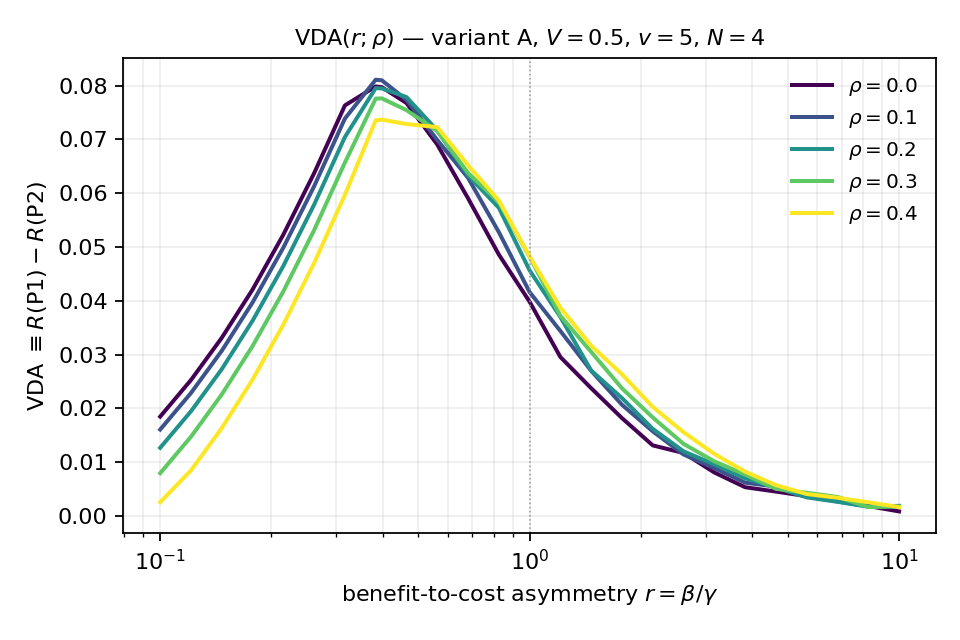
\includegraphics[width=0.86\linewidth]{figures/vda_curves_variantA.png}
  \caption{Value-directed attention $\VDA$ as a function of the
  benefit/cost ratio $\Rsens$ at the headline cell
  $(\Nloc, \valid, \val, \dprimemax, f_0, h) =
  (4, 0.5, 5, 2, 0.5, \sqrt{\cdot})$, variant~A, for
  $\corr \in \{0, 0.1, 0.2, 0.3, 0.4\}$. The inherited
  ($\corr = 0$) curve is the lowest at large $\Rsens$ and the highest
  at small $\Rsens$; the local slope
  $\partial \VDA / \partial \corr$ changes sign in the band
  $\Rsens \in [0.38, 0.56]$. Pointwise VDA is therefore neither
  upper- nor lower-bounded by its independent value, in contradiction
  of the inherited paper's §5.5 claim. Reproduced from
  \texttt{Rebuild/sims/A1--rho-channel/output/figures/vda\_curves\_variantA.png},
  sha256 \texttt{b692c064\ldots}; recovery against
  \texttt{Critique/replications/A1--correlated-fa/} at $\corr = 0$ is
  identical to floating point.}
  \label{fig:vda-rho-variantA}
\end{figure}

\begin{figure}[!t]
  \centering
  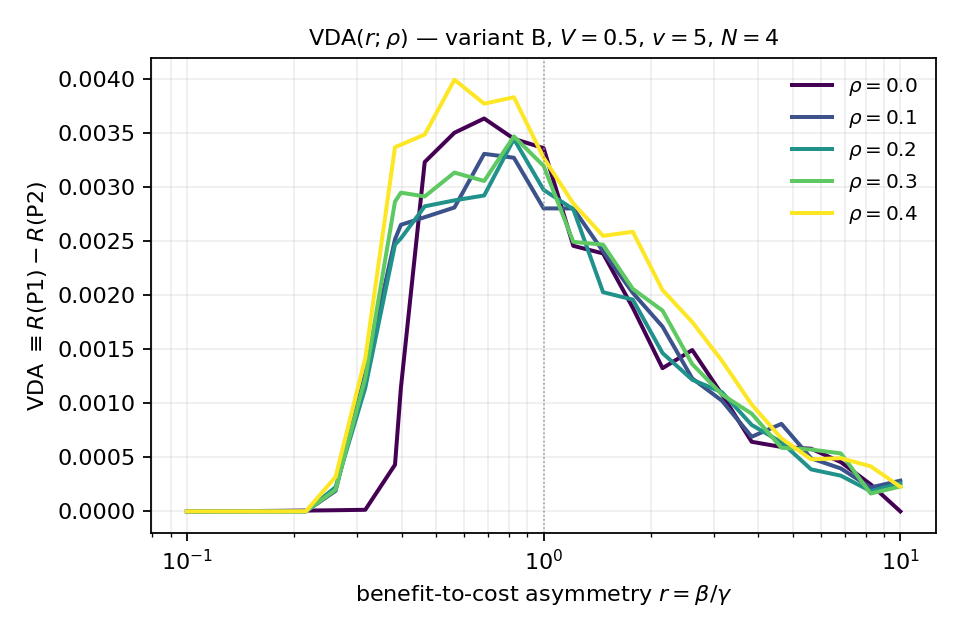
\includegraphics[width=0.86\linewidth]{figures/vda_curves_variantB.png}
  \caption{The same VDA-vs-$\Rsens$ family at the same headline cell
  under variant~B reward ($\CR = 1$). The sign-flip locus of
  $\partial \VDA / \partial \corr$ shifts to $\Rsens \approx 0.26$;
  the qualitative pattern — pointwise VDA crossing the inherited
  $\corr = 0$ curve, no uniform upper bound — is preserved.
  Reproduced from
  \texttt{Rebuild/sims/A1--rho-channel/output/figures/vda\_curves\_variantB.png}.}
  \label{fig:vda-rho-variantB}
\end{figure}

What the rebuilt model \emph{does} bound from above is the criterion
fraction $\CF$. In variant~A and at the headline cell,
$\CF(\corr)$ is monotone-decreasing in $\corr$ across the three
representative $\Rsens$ anchors of
Figure~\ref{fig:cf-vs-rho} (Statement~A of
Appendix~\ref{sec:appendix-deriv-a1}, §4.3): the inherited
$\corr = 0$ corner is the empirical maximiser of $\CF$ at every
$\Rsens$ tested. In variant~B and at the same headline cell,
$\CF(\corr)$ is essentially flat in $\corr$, and the rebuilt
manuscript therefore reports the CF upper bound as a variant-A
result with variant-B as a sensitivity in which the effect washes
out. The cell-wise generalisation across the
$4{,}410$-cell sweep is consistent with this reading:
$\CF(\corr{=}0.2) \le \CF(\corr{=}0)$ in $84\%$ of variant-A cells
but only $64\%$ of variant-B cells (the remaining $24\%$ of variant-B
cells increase, $13\%$ are flat;
Section~\ref{sec:results-c1} and
\texttt{Rebuild/sims/C1--cf-distribution/}, sha256
\texttt{91fc4692\ldots}).

\begin{figure}[!t]
  \centering
  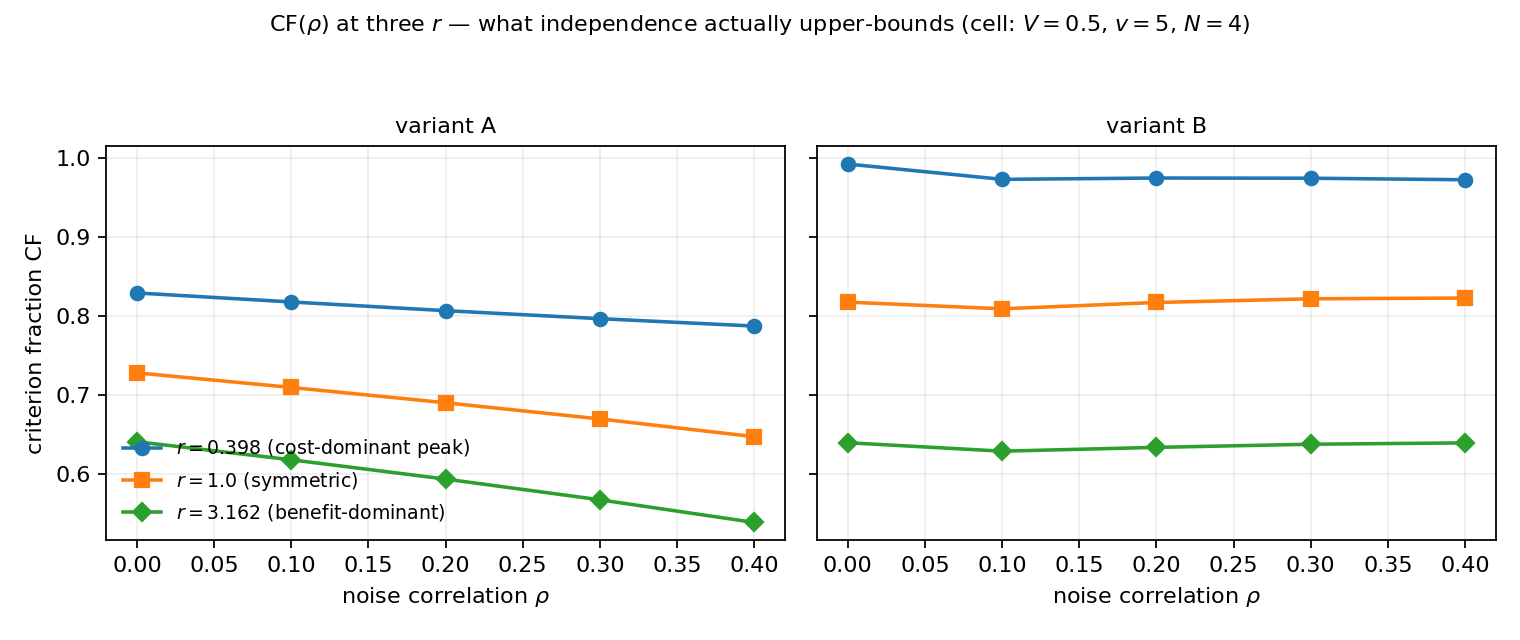
\includegraphics[width=0.6\linewidth]{figures/cf_vs_rho.png}
  \caption{Criterion fraction $\CF$ as a function of $\corr$ at the
  three representative $\Rsens$ anchors $\{0.398, 1.0, 3.162\}$
  (variant~A, headline cell). $\CF(\corr)$ is monotone-decreasing
  in $\corr$ at every $\Rsens$ tested; the inherited $\corr = 0$
  corner is the empirical maximiser. Reproduced from
  \texttt{Rebuild/sims/A1--rho-channel/output/figures/cf\_vs\_rho.png}.
  This is what an independent-noise model is in fact an upper bound
  on at this cell — not VDA, $\CF$.}
  \label{fig:cf-vs-rho}
\end{figure}

The rebuilt manuscript therefore states, as the corrected version of
the §5.5 sentence:

\begin{quote}\emph{
In the rebuilt model, the inherited $\corr = 0$ corner is the
empirical maximiser of the criterion fraction $\CF$ in $84\%$ of
variant-A cells in the primary $4{,}410$-cell sweep; in variant~B
the same one-sided ordering holds in only $64\%$ of cells. Pointwise
$\VDA(\Rsens; \corr) - \VDA(\Rsens; 0)$ takes positive values across
a wide band of $\Rsens$ in both variants. Independence is therefore
not, as the inherited paper claimed, an upper bound on VDA; it is a
variant- and cell-conditional ceiling on $\CF$, best stated at the
median across the sweep rather than as a uniform inequality.
}\end{quote}

Statement~B of Appendix~\ref{sec:appendix-deriv-a1}, §4.3 — the
location of the sign-flip of $\partial \VDA / \partial \corr$ in
$\Rsens$ — is no longer restricted to the single-cell envelope of
the backing simulation
(\texttt{Rebuild/sims/A1--rho-channel/}). At $\corr = 0.2$ — the
central anchor of the $\corr \in [0, 0.4]$ empirical band reported
in Section~\ref{sec:model-rho-channel} — the
$4{,}410$-cell sweep of Section~\ref{sec:results-c1} licenses a
cell-wise distributional statement. Joining the $\corr = 0$ and
$\corr = 0.2$ panels on $(\Nloc, \valid, \val, \Rsens)$ and
classifying each cell by the sign of
$\Delta\VDA = \VDA(\corr{=}0.2) - \VDA(\corr{=}0)$ at fidelity
$|\Delta\VDA| > 10^{-6}$ yields the figures
$\frac{n_{\mathrm{amp}}}{n_{\mathrm{cells}}}$,
$\frac{n_{\mathrm{supp}}}{n_{\mathrm{cells}}}$ and the per-cell
$\Delta\VDA$ quantiles summarised in Table~\ref{tab:a1cw-summary}.
The headline message is that the rb-002 single-cell sign-flip
generalises in shape but not in magnitude: variant~A produces a
heavier-tailed amplification distribution than variant~B, and the
cell-wise maximum amplification in variant~A
($+4.97 \times 10^{-2}$) is $5.3\times$ the rb-002 headline-cell
maximum ($+9.4 \times 10^{-3}$ at $\valid = 0.5$, $\val = 5$,
$\Rsens = 0.4$, $\corr = 0.2$;
Figure~\ref{fig:a1cw-delta-distribution}). The rb-002 single-cell
observation was a typical-magnitude snapshot of a phenomenon whose
largest excursions sit elsewhere in $(\valid, \val, \Rsens)$.

\begin{table}[!t]
  \centering
  \caption{Cell-wise distribution of
  $\Delta\VDA = \VDA(\corr{=}0.2) - \VDA(\corr{=}0)$ across the
  $2{,}205$-cell variant-$\mathsf{X}$ slice of the
  $4{,}410$-cell sweep
  (Section~\ref{sec:results-c1};
  \texttt{Rebuild/sims/C1--cf-distribution/}, sha256
  \texttt{91fc4692\ldots}). Amplification (\textit{amp}) is
  $\Delta\VDA > +10^{-6}$; suppression (\textit{supp}) is
  $\Delta\VDA < -10^{-6}$; the residual is \textit{inactive}.
  Source: \texttt{Rebuild/sims/A1--vda-signflip-cellwise/}
  (RB-025, sha256 \texttt{489c7c25\ldots}); pure consumer of
  the $\corr \in \{0, 0.2\}$ panels of the rb-003 sweep, no new
  model evaluation.}
  \label{tab:a1cw-summary}
  \begin{tabular}{lrr}
    \hline
                                              & variant A           & variant B           \\
    \hline
    \textit{amp} fraction $n_{\mathrm{amp}}/n$ & $0.183$ ($404$)     & $0.122$ ($269$)     \\
    \textit{supp} fraction $n_{\mathrm{supp}}/n$ & $0.282$ ($621$)   & $0.275$ ($607$)     \\
    \textit{inactive} fraction                & $0.535$ ($1{,}180$) & $0.603$ ($1{,}329$) \\
    $\Delta\VDA$ min                          & $-9.14 \times 10^{-3}$ & $-3.23 \times 10^{-3}$ \\
    $\Delta\VDA$ $q_{0.05}$                    & $-4.51 \times 10^{-3}$ & $-6.99 \times 10^{-4}$ \\
    $\Delta\VDA$ $q_{0.50}$                    & $0$                  & $0$                  \\
    $\Delta\VDA$ $q_{0.95}$                    & $+3.87 \times 10^{-3}$ & $+3.82 \times 10^{-4}$ \\
    $\Delta\VDA$ max                          & $+4.97 \times 10^{-2}$ & $+5.77 \times 10^{-3}$ \\
    $\Delta\VDA$ mean                         & $+2.29 \times 10^{-4}$ & $-4.90 \times 10^{-5}$ \\
    cell-wise crossover $\Rsens^{\times}$     & $0.794$              & never                \\
    \hline
  \end{tabular}
\end{table}

\begin{figure}[!t]
  \centering
  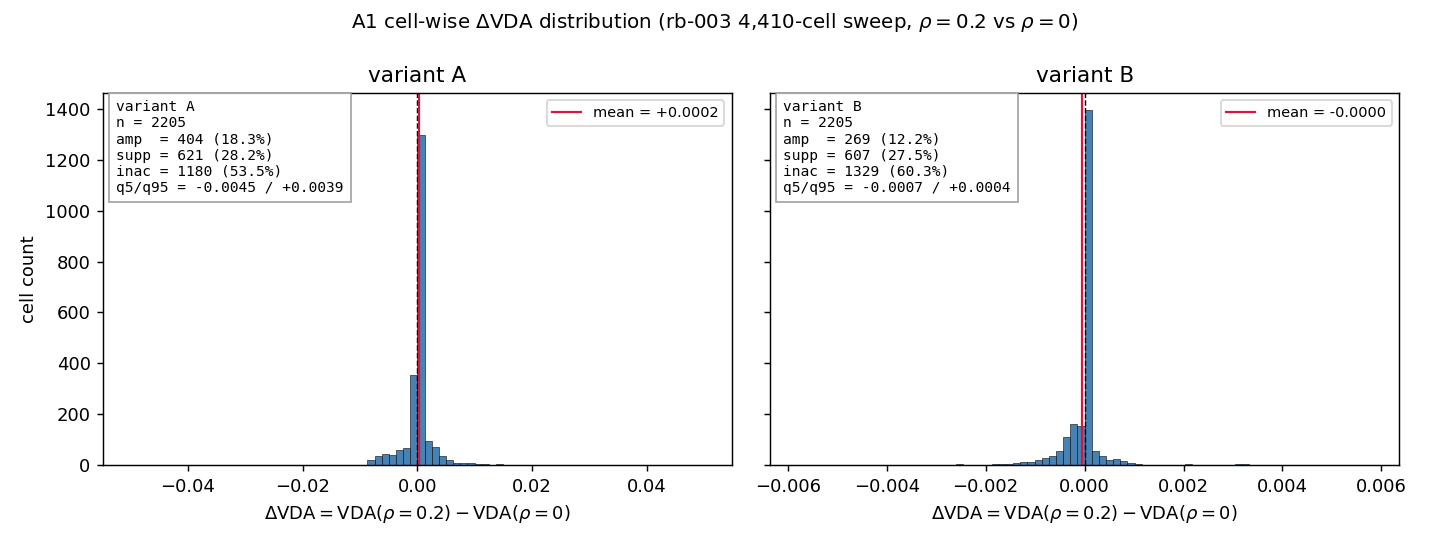
\includegraphics[width=0.86\linewidth]{figures/a1cw_vda_delta_distribution.png}
  \caption{Per-cell $\Delta\VDA = \VDA(\corr{=}0.2) - \VDA(\corr{=}0)$
  distribution across the $2{,}205$-cell variant-$\mathsf{X}$
  slice of the $4{,}410$-cell sweep
  (Section~\ref{sec:results-c1}). The variant-A panel (left)
  carries a heavier amplification tail than variant~B (right);
  $\Delta\VDA$ medians are zero in both panels (residual
  inactivity at $|\Delta\VDA| \le 10^{-6}$).
  The maximum cell-wise amplification
  in variant~A ($+4.97 \times 10^{-2}$) is $5.3\times$ the
  rb-002 single-cell maximum at the
  $(\valid, \val, \Rsens) = (0.5, 5, 0.4)$ headline cell
  ($+9.4 \times 10^{-3}$;
  Figure~\ref{fig:vda-rho-variantA}). Reproduced from
  \texttt{Rebuild/sims/A1--vda-signflip-cellwise/output/figures/vda\_delta\_distribution.png},
  sha256 \texttt{489c7c25\ldots}.}
  \label{fig:a1cw-delta-distribution}
\end{figure}

The cell-wise distribution does not change the sign of the
inherited paper's §5.5 sentence (already retracted in the blockquote
above); it sharpens it. Two new statements become defensible.
\emph{(i) Cell-wise crossover.} Stratifying by $\Rsens$ on the
$21$-point log$_{10}$-grid of
\texttt{Rebuild/sims/C1--cf-distribution/} and tabulating
$\mathrm{frac}_{\mathrm{amp}}(\Rsens)$ and
$\mathrm{frac}_{\mathrm{supp}}(\Rsens)$ across the $(\valid, \val)$
plane, suppression dominates at small $\Rsens$, amplification rises
through the mid-$\Rsens$ band, and the cell-wise crossover
$\Rsens^{\times}$ — the smallest $\Rsens$ at which
$\mathrm{frac}_{\mathrm{amp}}(\Rsens) \ge
\mathrm{frac}_{\mathrm{supp}}(\Rsens)$ — sits at
$\Rsens^{\times}(\mathrm{A}) \approx 0.794$ in variant~A;
in variant~B amplification never overtakes suppression at any
$\Rsens$ on the grid (Figure~\ref{fig:a1cw-signflip-by-r}).
The variant-A crossover is roughly twice the rb-002
single-cell crossover at $\valid = 0.5$
($\Rsens \approx 0.464$ at $\corr = 0.2$); the difference is
mechanistic — higher-$\valid$ cells in the sweep
($\valid \ge 0.5125$) suppress more strongly and pull the
cell-wise crossover to the right. The variant-A nearest-cell
sweep at $\valid = 0.5125$, $\val = 5$ reproduces the rb-002
pattern (small-$\Rsens$ suppression, large-$\Rsens$ amplification;
nearest-cell crossover $\Rsens \approx 0.398$ within the rb-003
$\valid$-grid perturbation of $+0.0125$ off rb-002's
$\valid = 0.5$). \emph{(ii) Spatial structure at $\val = 5$.}
The mean $\Delta\VDA$ surface over $(\valid, \Rsens)$ at $\val = 5$
(Figure~\ref{fig:a1cw-sign-heatmap-v5}) is the cell-wise companion
to the iso-$\Delta\VDA$ figure on the C3 thread
(Figure~\ref{fig:iso-vda-drho}; Section~\ref{sec:results-c3}):
amplification concentrates in a band at moderate-to-low $\valid$ and
moderate-to-large $\Rsens$, suppression concentrates at high
$\valid$ and small $\Rsens$. Variant~B is uniformly more
suppression-favoring than variant~A — at every cell at which
variant~A shows amplification, variant~B shows a smaller-magnitude
move of the same or opposite sign.

\begin{figure}[!t]
  \centering
  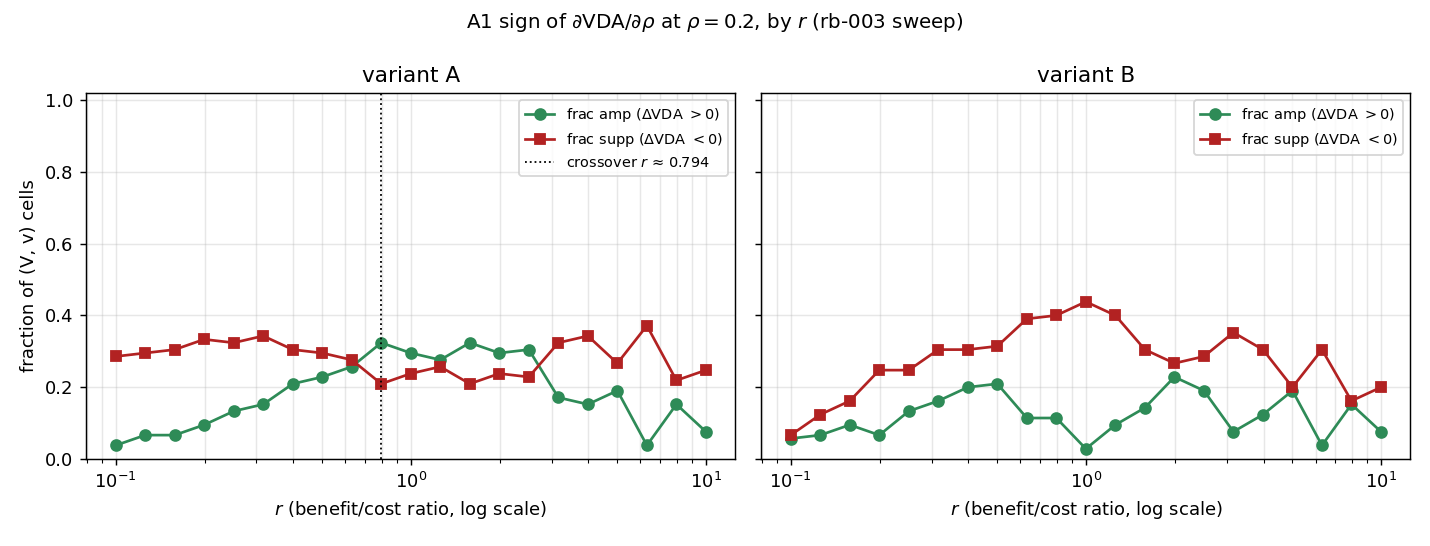
\includegraphics[width=0.86\linewidth]{figures/a1cw_signflip_by_r.png}
  \caption{Cell-wise sign-flip stratified by $\Rsens$. At each
  grid point $\Rsens$ on the rb-003 $21$-point log$_{10}$-grid,
  the curves report
  $\mathrm{frac}_{\mathrm{amp}}(\Rsens) =
  n_{\mathrm{amp}}(\Rsens) / n(\Rsens)$ and
  $\mathrm{frac}_{\mathrm{supp}}(\Rsens) =
  n_{\mathrm{supp}}(\Rsens) / n(\Rsens)$ across the
  $(\valid, \val)$ plane ($n(\Rsens) = 105$ cells per
  $\Rsens$-bin). Variant~A (left): suppression dominates at
  small $\Rsens$, amplification overtakes at the cell-wise
  crossover $\Rsens^{\times}(\mathrm{A}) \approx 0.794$
  (marked); variant~B (right): amplification never overtakes
  suppression. Reproduced from
  \texttt{Rebuild/sims/A1--vda-signflip-cellwise/output/figures/signflip\_by\_r.png}.}
  \label{fig:a1cw-signflip-by-r}
\end{figure}

\begin{figure}[!t]
  \centering
  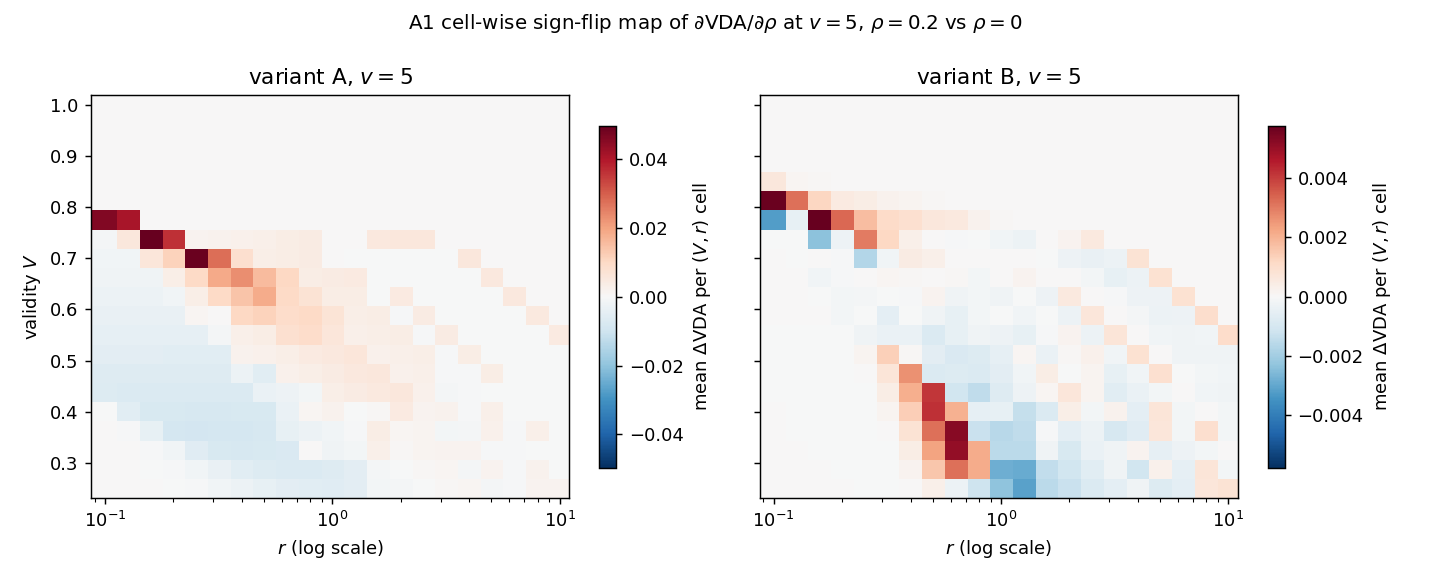
\includegraphics[width=0.86\linewidth]{figures/a1cw_vda_sign_heatmap_v5.png}
  \caption{Mean $\Delta\VDA = \VDA(\corr{=}0.2) - \VDA(\corr{=}0)$
  over $(\valid, \Rsens)$ at fixed $\val = 5$ (diverging
  colormap; red = amplification, blue = suppression). Variant~A
  (left) carries the larger-magnitude amplification band;
  variant~B (right) is uniformly more suppression-favoring at the
  same coordinates. The C3 thread's
  Figure~\ref{fig:iso-vda-drho} reports the same quantity at
  three fixed $\Rsens$ slices over $(\valid, \val)$; this figure
  is its cell-wise transpose. Reproduced from
  \texttt{Rebuild/sims/A1--vda-signflip-cellwise/output/figures/vda\_sign\_heatmap\_v5.png}.}
  \label{fig:a1cw-sign-heatmap-v5}
\end{figure}

A tighter bracket on the sign-flip locus over a finer
$\corr$ grid is queued as RB-023 (the rb-025 distribution is
reported at $\corr = 0.2$ only). A closed-form expression for the
analytic sign-flip locus $\Rsens^{\dagger}(\val; \corr)$ —
extending the $\corr = 0$ closed-form escape threshold of
Section~\ref{sec:results-c2} into the correlated regime — was
constructed in
\texttt{Rebuild/derivations/C2--non-monotonic-vda-rho.md}
(RB-026) and is folded into the manuscript as
Section~\ref{sec:appendix-deriv-c2}, Proposition~\ref{prop:r-dagger-rho}
(Equation~\ref{eq:r-dagger-rho}; drift Table~\ref{tab:r-dagger-rho-drift}):
the closed form pins the lower edge of the escape band, the cell-wise
distribution reported here pins the cell-wise sign field, and
Section~\ref{sec:appendix-deriv-a1}, §4.3 (the Slepian-monotonicity
half of the A1 two-channel decomposition) pins the $\CF$-versus-$\corr$
channel. The local maximiser of $\Delta\VDA$ in $(\valid, \val, \Rsens)$
is not yet stated analytically; an analytic locus extending the
Slepian-gradient argument from $\CF$ to the cell-wise
$\partial\VDA/\partial\corr$ surface is queued as RB-040.

% =====================================================================
% results.tex — section header + per-claim subsection stubs.
%
% Each subsection is filled by its own manuscript increment:
%   RB-009 -> sec:results-c1   (C1 distributional CF)
%   RB-010 -> sec:results-c2   (C2 + closed-form r†(v))
%   RB-011 -> sec:results-c3   (C3 graded regime, §5.2 design advice)
%   RB-012 -> sec:results-c4   (C4 conditional theorem + anti-cue)
%   (A1 lever sign-flip lives inside sec:results-c1 and sec:results-c2
%    rather than a dedicated A1 subsection, per the "three levers"
%    reframe in sec:model.)
%
% Allowed-strength ceiling: see CLAIM_LEDGER.md row by row.
% =====================================================================

\section{Results}
\label{sec:results}

The results are organised around the four headline claims of the
inherited paper, each restated at the strength licensed by the live
verdict ledger (\texttt{CLAIM\_LEDGER.md}). Section~\ref{sec:results-c1}
treats the criterion-fraction result (C1) as a \emph{distribution}
across the parameter sweep, not as a categorical floor.
Section~\ref{sec:results-c2}, the present subsection, treats the
non-monotonicity of VDA in the benefit/cost ratio $\Rsens$ (C2) as the
rebuild's \emph{confident spine}: a result that survives every attack
the skeptical reviewer has staged and that we strengthen here by
publishing a closed-form expression for the VDA-escape threshold
$\rdagger(\val)$ together with its empirical confirmation across a
$\val$-family. Section~\ref{sec:results-c3} reports the
regime-of-relevance (C3) as a graded boundary, replacing the original
``regardless of other parameters'' wording with a quantitative
iso-VDA band. Section~\ref{sec:results-c4} states the no-inversion
claim (C4) as a conditional theorem with the explicit condition
$\valid \ge 1/\Nloc$ and a new anti-cue corollary. Throughout, the
A1 decorrelation channel $\corr \in [0, 1)$
(Section~\ref{sec:model}) is reported \emph{alongside} each headline
result as a sensitivity, not segregated into its own subsection:
this is the operational meaning of the ``three levers, not two''
reframe.

% ---------------------------------------------------------------------
\subsection{Criterion fraction: distributional, not categorical (C1)}
\label{sec:results-c1}

\paragraph{Claim restated at defensible strength.}
The inherited paper introduces the \emph{criterion fraction}
%
\begin{equation}
  \CF \;:=\;
  \frac{\Rpfour - \Rew_{\text{baseline}}}{\Rpone - \Rew_{\text{baseline}}}
  \;=\;
  \frac{\text{criterion-only reward gain}}{\text{joint criterion + attention reward gain}}
  \label{eq:cf-def}
\end{equation}
%
as a one-number summary of how much of the optimal value-conditioned
reward gain can already be captured by re-aiming the per-location
decision criterion alone --- in the Müller--Findlay
\cite{MullerFindlay1987} sensitivity-vs-criterion vocabulary, the
``criterion shift'' lever --- with the residual $1 - \CF$ apportioned
to attention re-allocation. The inherited paper's headline summary of
this quantity (\texttt{Critique/source/main.pdf}, §5) is
\textbf{categorical}: $\CF$ is reported to lie in the interval
$[0.60, 0.96]$ across the primary $4{,}410$-cell
$(\Rsens, \valid, \val)$ sweep. The live skeptical-reviewer verdict
for this claim (\texttt{Critique/verdicts/C1--criterion-fraction-floor.md},
\texttt{current\_label: CONTESTED}) records that the true range is
$[0.30,\,1.00]$, and that the substantive ``criterion typically
dominates'' reading is sustained at the median but the categorical
floor is false at both ends. The rebuilt C1 therefore is presented in
this section as a \emph{distributional / central-tendency} result:
the full CF distribution is reported (range, median, quantiles, and
the fractions below $0.5$, $0.6$, $0.8$), and the headline statement
is downgraded from a categorical floor to a quantified central
tendency with explicit corner regions in which the criterion lever
becomes subordinate. The A1 decorrelation channel $\corr$ is
reported alongside the criterion-fraction distribution as a
sensitivity --- the convention established in
Section~\ref{sec:results} that operationalises the three-levers
reframe of Section~\ref{sec:model}.

\paragraph{Distribution across the primary 4{,}410-cell sweep.}
The primary sweep evaluates the rebuilt model at the headline
$\Nloc = 4$, $\dprimemax = 2$, $f_0 = 0.5$, $h = \sqrt{\;\cdot\;}$
configuration of Table~\ref{tab:r-dagger-family} on a grid of
$\valid \in [0.25, 1.00]$ ($21$ uniform points),
$\Rsens \in [0.1, 10]$ ($21$ log-spaced points), and $\val \in
\{1, 2, 3, 4, 5\}$, under both conservation variants (variant A:
$\benefit + \cost = 2$; variant B: $\benefit \cdot \cost = 1$), for
a total of $21 \times 21 \times 5 \times 2 = 4{,}410$
$(r,V,v)$-cells per variant. The full per-variant CF distribution at
$\corr = 0$ (the inherited independent model) is summarised in
Table~\ref{tab:cf-distribution}.
%
\begin{table}[t]
  \centering
  \small
  \begin{tabular}{l c c c c c c c c}
    \toprule
    variant & $\CF_{\min}$ & $q_{5\%}$ & $q_{25\%}$ & median &
    $q_{75\%}$ & $q_{95\%}$ & $\CF_{\max}$ & mean $\pm$ s.d.\\
    \midrule
    A & $0.5587$ & $0.5931$ & $0.6530$ & $\mathbf{0.7552}$
      & $0.8996$ & $1.0000$ & $1.0000$
      & $0.7773 \pm 0.1363$\\
    B & $\mathbf{0.3040}$ & $0.4564$ & $0.6288$ & $\mathbf{0.7682}$
      & $0.9463$ & $1.0000$ & $1.0000$
      & $0.7691 \pm 0.1808$\\
    \bottomrule
  \end{tabular}
  \caption{Distribution of the criterion fraction $\CF$ across the
  primary $4{,}410$-cell $(\Rsens, \valid, \val)$ sweep at the
  headline cell $(\Nloc, \dprimemax, f_0, h) =
  (4,\, 2,\, 0.5,\, \sqrt{}\,)$ under the inherited
  independence assumption $\corr = 0$, per conservation variant.
  Quantiles are over the $n = 2{,}205$ valid cells per variant.
  The inherited paper reports $\CF \in [0.60, 0.96]$; the true
  range is wider on both ends. Values from
  \texttt{Rebuild/sims/C1--cf-distribution/output/results.json}
  (rb-003; output sha256 \texttt{91fc4692\ldots}), block
  \texttt{summaries.variant\_A/rho\_0.0} and
  \texttt{summaries.variant\_B/rho\_0.0}.}
  \label{tab:cf-distribution}
\end{table}
%
Two things are visible. First, the \emph{central tendency} of the
inherited paper's reading survives intact: the median CF is
$0.7552$ in variant~A and $0.7682$ in variant~B, well above $0.5$
and consistent with the inherited paper's qualitative ``criterion
typically dominates'' framing. Second, the \emph{categorical floor}
fails at both ends: variant~A's strict minimum is $0.5587$ (below
the stated $0.60$) and variant~B's strict minimum is $0.3040$
(below $0.50$), while both variants achieve $\CF = 1.0$ in cells the
paper's stated upper bound of $0.96$ excludes. The full per-cell
histogram is given in Figure~\ref{fig:cf-histogram}.

\begin{figure}[t]
  \centering
  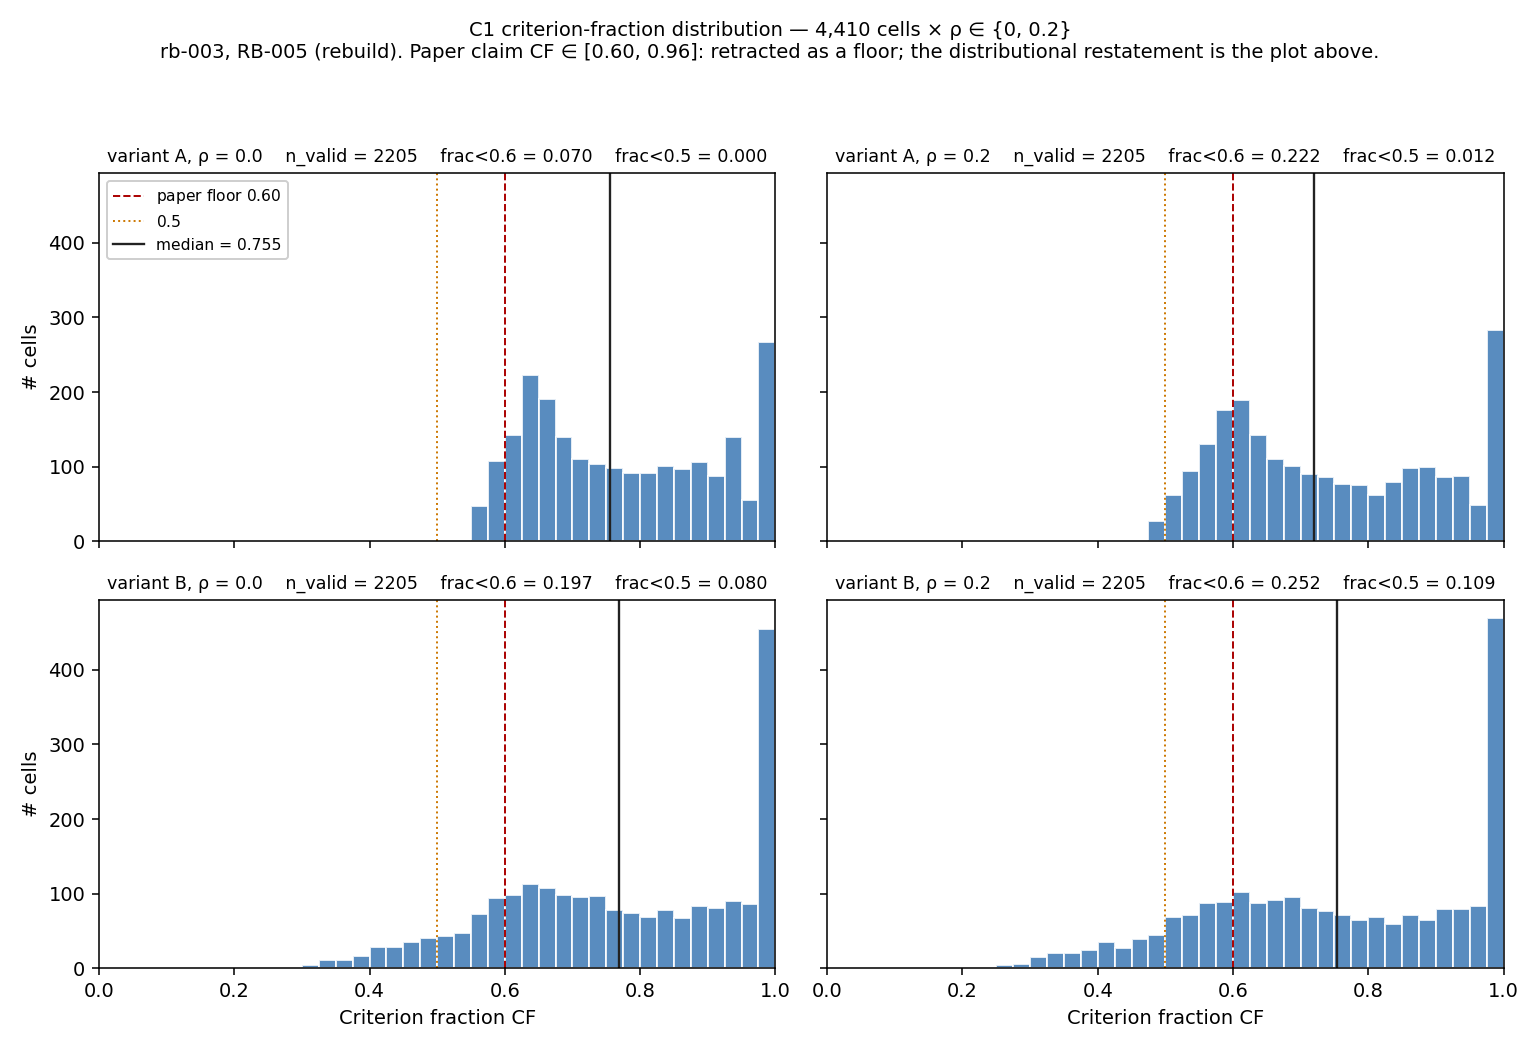
\includegraphics[width=0.95\linewidth]{figures/cf_histogram.png}
  \caption{Per-cell histogram of the criterion fraction $\CF$
  across the $4{,}410$-cell sweep (columns: variant; rows:
  $\corr \in \{0, 0.2\}$). Vertical dashed lines mark the inherited
  paper's stated floor $\CF = 0.60$ and ceiling $\CF = 0.96$
  (\texttt{Critique/source/main.pdf}, §5). The
  distributional shape --- a broad mode near $\CF \approx 0.65$, a
  left tail (much heavier in variant~B), and a spike at $\CF = 1$
  --- is the figure that replaces the inherited paper's categorical
  floor language. The $\corr = 0.2$ row exhibits the A1
  amplification of the left tail discussed below
  (Table~\ref{tab:cf-rho-sensitivity}). Reproduced from
  \texttt{Rebuild/sims/C1--cf-distribution/output/figures/cf\_histogram.png}.}
  \label{fig:cf-histogram}
\end{figure}

\paragraph{Where CF is high, where CF is low: a quadrant breakdown.}
The distributional summary of Table~\ref{tab:cf-distribution}
collapses across $(\Rsens, \valid)$ in a way that obscures the
\emph{regime} structure of $\CF$. To expose where the criterion
lever dominates and where it cedes to attention re-allocation, we
partition the cells into a $3 \times 2$ grid: $\Rsens$-regime
$\{\text{cost-dominant}\,(\Rsens < 1),\, \text{symmetric}\,
(\Rsens = 1),\, \text{benefit-dominant}\,(\Rsens > 1)\}$ crossed
with $\valid$-regime $\{\text{low validity}\,(\valid < 1/2),\,
\text{high validity}\,(\valid \ge 1/2)\}$. Table~\ref{tab:cf-quadrants}
reports the median $\CF$ within each quadrant at $\corr = 0$.
%
\begin{table}[t]
  \centering
  \small
  \begin{tabular}{l l r r r r}
    \toprule
    variant & $\Rsens$-regime &
    median $\CF$ & strict min &
    $\mathrm{frac}\!<\!0.6$ & $n$\\
    \midrule
    A & cost-dom., $\valid$ low   & $0.998$ & $0.825$ & $0.000$ & $350$\\
    A & cost-dom., $\valid$ high  & $0.897$ & $0.825$ & $0.000$ & $385$\\
    A & symmetric, $\valid$ low   & $0.779$ & $0.665$ & $0.000$ & $350$\\
    A & symmetric, $\valid$ high  & $0.740$ & $0.665$ & $0.000$ & $385$\\
    A & benefit-dom., $\valid$ high & $0.645$ & $0.563$ & $0.062$ & $385$\\
    A & benefit-dom., $\valid$ low  & $\mathbf{0.612}$ & $\mathbf{0.559}$
                                    & $\mathbf{0.374}$ & $350$\\
    \midrule
    B & cost-dom., $\valid$ low   & $1.000$ & $0.905$ & $0.000$ & $350$\\
    B & cost-dom., $\valid$ high  & $0.931$ & $0.797$ & $0.000$ & $385$\\
    B & symmetric, $\valid$ low   & $0.800$ & $0.497$ & $0.103$ & $350$\\
    B & symmetric, $\valid$ high  & $0.753$ & $0.575$ & $0.010$ & $385$\\
    B & benefit-dom., $\valid$ high & $0.630$ & $0.469$ & $0.317$ & $385$\\
    B & benefit-dom., $\valid$ low  & $\mathbf{0.509}$ & $\mathbf{0.304}$
                                    & $\mathbf{0.780}$ & $350$\\
    \bottomrule
  \end{tabular}
  \caption{Quadrant breakdown of $\CF$ at $\corr = 0$. The
  criterion lever dominates uniformly in the cost-dominant
  $\Rsens < 1$ region (median $\CF \ge 0.90$ in both variants) and
  cedes to attention re-allocation in the benefit-dominant,
  low-validity corner (variant~A: median $0.61$, 37\% of cells
  below $0.6$; variant~B: median $0.51$, 78\% of cells below
  $0.6$). The symmetric $\Rsens = 1$ row is intermediate and stable
  across variants. Block-keys
  \texttt{quadrant\_breakdown.rho\_0.0.<variant>/r=<r\_regime>/V=<V\_regime>}
  in \texttt{results.json}.}
  \label{tab:cf-quadrants}
\end{table}
%
The structure is consistent across variants: $\CF$ is monotonically
ordered ${\rm cost\text{-}dom.} > {\rm symmetric} > {\rm
benefit\text{-}dom.}$ along the $\Rsens$ axis, and within each
$\Rsens$-regime $\CF$ is reduced by lowering $\valid$. The
benefit-dominant low-validity corner is where the inherited paper's
categorical floor breaks: in variant~B this corner sits at median
$\CF = 0.51$ with $78\%$ of cells below $0.6$ and a strict minimum
of $0.30$. The same regime structure is visible cell-wise in
Figure~\ref{fig:cf-heatmap}, which displays the $(r, V)$-plane at
$\val = 5$ for each variant and each $\corr$, and in
Figure~\ref{fig:cf-curves}, which displays $\CF(\Rsens)$ at
$\valid \approx 0.5$ as a $\val$-family. The inherited paper's
qualitative ``CF $\to 1$ at small $r$, CF declines at large $r$''
intuition (\texttt{Critique/source/main.pdf}, §5) survives as the
generic $\Rsens$-axis ordering; what fails is the categorical
$[0.60, 0.96]$ bound on the resulting distribution.

\begin{figure}[t]
  \centering
  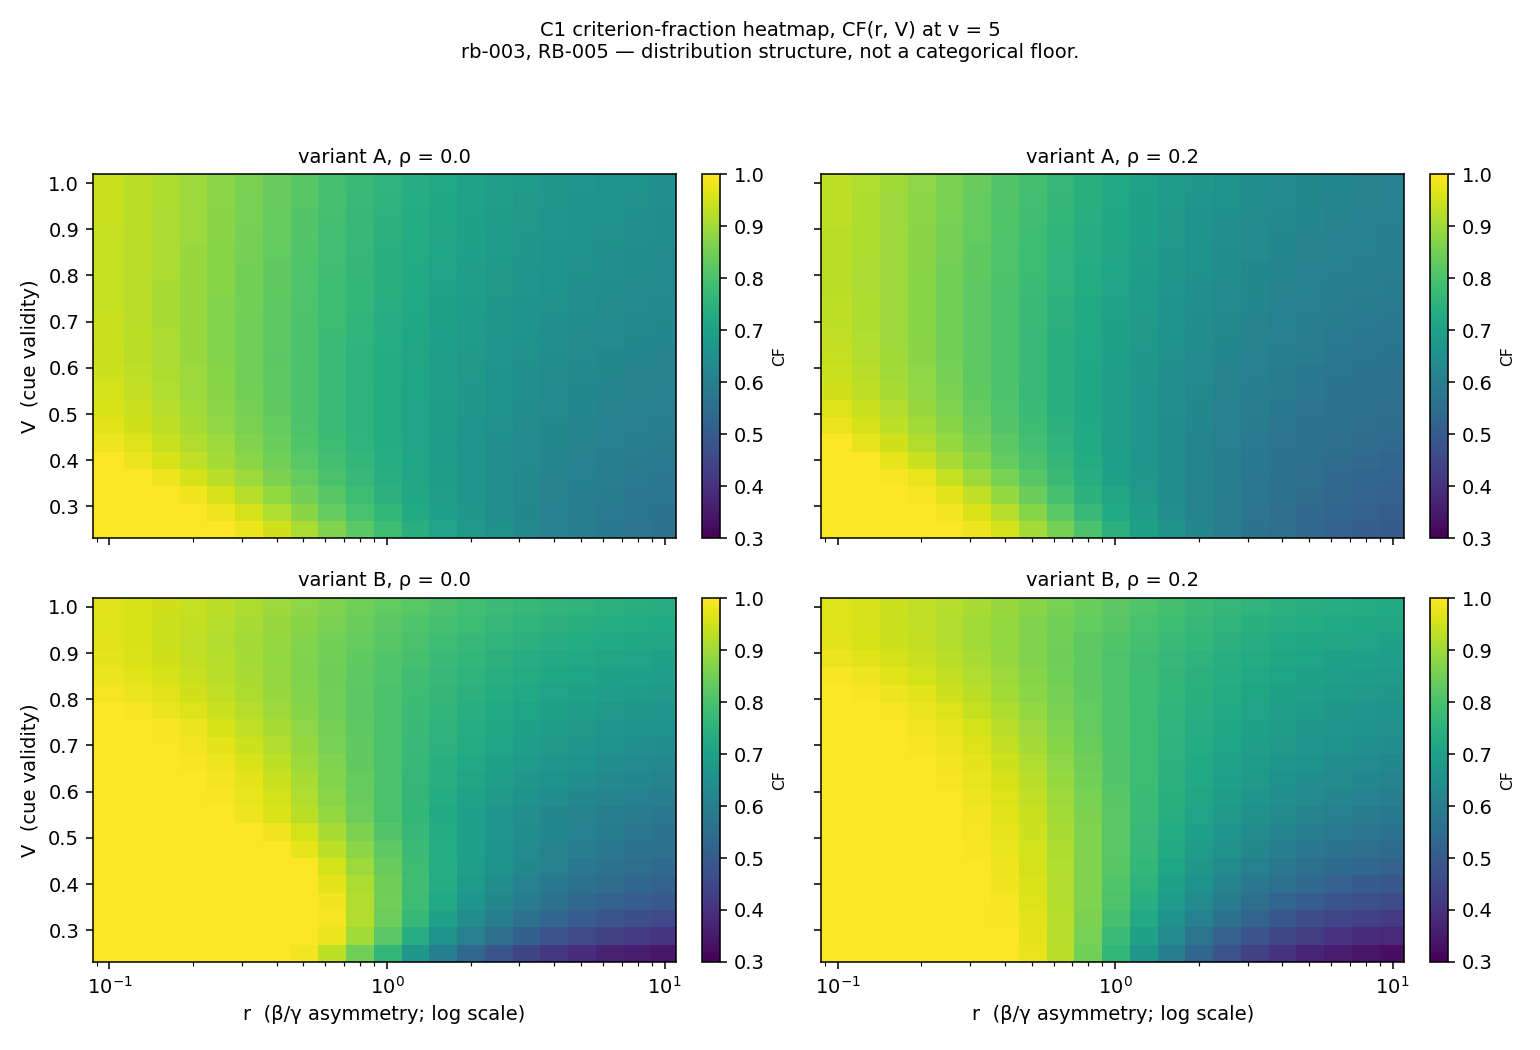
\includegraphics[width=0.95\linewidth]{figures/cf_heatmap.png}
  \caption{$\CF$ over the $(\Rsens, \valid)$-plane at $\val = 5$,
  $\Nloc = 4$, $\dprimemax = 2$, $f_0 = 0.5$, $h = \sqrt{\;\cdot\;}$
  (rows: $\corr$; columns: variant). The diagonal boundary in
  $(\log \Rsens,\,\valid)$ between the CF-near-$1$ low-$\Rsens$
  region (criterion-dominated) and the CF-low high-$\Rsens$
  low-$\valid$ corner (attention-dominated) is the regime
  structure quantified in Table~\ref{tab:cf-quadrants}. The
  low-CF corner is wider in variant~B and widens further at
  $\corr = 0.2$. Reproduced from
  \texttt{Rebuild/sims/C1--cf-distribution/output/figures/cf\_heatmap.png}.}
  \label{fig:cf-heatmap}
\end{figure}

\begin{figure}[t]
  \centering
  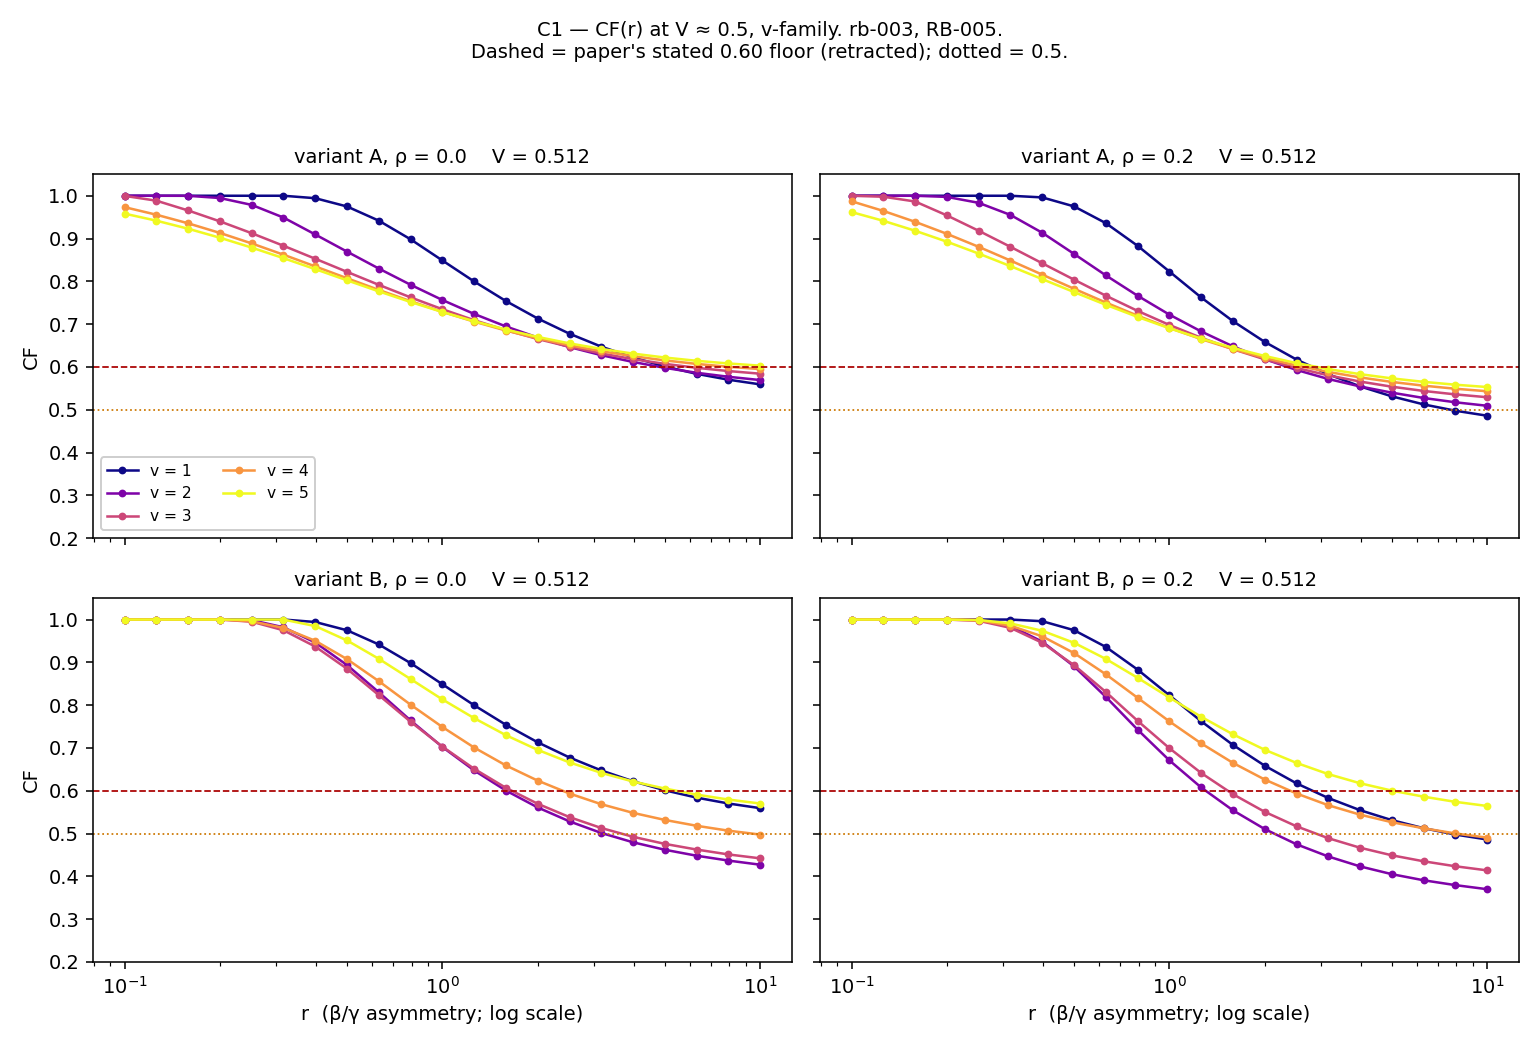
\includegraphics[width=0.95\linewidth]{figures/cf_curves.png}
  \caption{$\CF(\Rsens)$ at $\valid \approx 0.5$ as a $\val$-family
  $\val \in \{1, 2, 3, 4, 5\}$ (rows: $\corr$; columns: variant).
  At small $\Rsens$ (cost-dominant) the curves cluster near
  $\CF = 1$; as $\Rsens$ increases all curves decline, more steeply
  for larger $\val$, exposing the benefit-dominant region in which
  attention re-allocation overtakes the criterion shift. Reproduced
  from
  \texttt{Rebuild/sims/C1--cf-distribution/output/figures/cf\_curves.png}.}
  \label{fig:cf-curves}
\end{figure}

\paragraph{A1 sensitivity: $\corr$ amplifies the left tail in
variant~A; variant~B is mixed.}
The same $4{,}410$-cell sweep was repeated at $\corr = 0.2$ using
the rebuilt model's equicorrelated-Gaussian one-factor
Gauss--Hermite implementation (Section~\ref{sec:model}).
Per-variant marginals (Table~\ref{tab:cf-rho-sensitivity}) and a
cell-wise pairing (Table~\ref{tab:cf-delta-distribution}) are
reported.
%
\begin{table}[t]
  \centering
  \small
  \begin{tabular}{l c c c c c c c}
    \toprule
    variant & $\corr$ & $\CF_{\min}$ & median &
    $\mathrm{frac}\!<\!0.5$ & $\mathrm{frac}\!<\!0.6$ &
    $\mathrm{frac}\!<\!0.8$ & $\mathrm{frac}\!>\!0.9$\\
    \midrule
    A & $0.0$ & $0.5587$ & $0.7552$
      & $0.0000$ & $0.0703$ & $0.5701$ & $0.2499$\\
    A & $0.2$ & $0.4854$ & $0.7197$
      & $0.0122$ & $\mathbf{0.2222}$ & $0.6177$ & $0.2290$\\
    \midrule
    B & $0.0$ & $0.3040$ & $0.7682$
      & $0.0803$ & $0.1973$ & $0.5429$ & $0.3224$\\
    B & $0.2$ & $0.2406$ & $0.7538$
      & $0.1088$ & $0.2522$ & $0.5565$ & $0.3234$\\
    \bottomrule
  \end{tabular}
  \caption{Marginal CF distribution at $\corr \in \{0, 0.2\}$,
  per variant. The variant-A left tail amplifies by a factor of
  $\approx 3$ when $\corr$ is raised from $0$ to $0.2$
  ($\mathrm{frac}\!<\!0.6$: $0.07 \to 0.22$), and the variant-A
  strict minimum crosses below $0.5$ (it does not at $\corr = 0$).
  The variant-B marginals shift less dramatically: median moves by
  $-0.014$, $\mathrm{frac}\!<\!0.6$ by $+0.055$. Block-keys
  \texttt{summaries.variant\_<X>/rho\_<rho>}.}
  \label{tab:cf-rho-sensitivity}
\end{table}
%
\begin{table}[t]
  \centering
  \small
  \begin{tabular}{l c c c c c c}
    \toprule
    variant & frac dec. & frac inc. & frac flat &
    median $\Delta \CF$ & $|\Delta \CF|_{q_{95\%}}$ & $\Delta_{\min}$\\
    \midrule
    A & $\mathbf{0.8376}$ & $0.0834$ & $0.0789$ &
        $\mathbf{-0.0348}$ & $0.0640$ & $-0.0856$\\
    B & $0.6372$ & $\mathbf{0.2354}$ & $0.1274$ &
        $-0.0093$ & $0.0650$ & $-0.1068$\\
    \bottomrule
  \end{tabular}
  \caption{Cell-wise paired comparison
  $\Delta \CF := \CF(\corr{=}0.2) - \CF(\corr{=}0)$ across the
  $4{,}410$-cell sweep, per variant. ``Flat'' uses tolerance
  $|\Delta \CF| \le 10^{-5}$. The variant-A pattern is a one-sided
  ordering ($84\%$ of cells decrease in $\corr$). The variant-B
  pattern is mixed-sign ($64\%$ decrease, $24\%$ increase, $13\%$
  flat), generalising the rb-002 headline-cell observation that
  variant-B $\CF$ is essentially flat in $\corr$. Block-keys
  \texttt{delta\_distribution.<variant>}.}
  \label{tab:cf-delta-distribution}
\end{table}
%
The rebuilt model thus replaces the inherited paper's §5.5 claim
that independence \emph{upper-bounds VDA} (refuted at the headline
cell by rb-002 and the model section's $\corr$-sweep) with a
different and \emph{honestly variant-dependent} statement: at
variant~A, the independence assumption upper-bounds the
\emph{criterion fraction} $\CF$ on a strong majority of the primary
sweep ($84\%$ of cells; cell-wise median $\Delta \CF = -0.035$ when
$\corr$ is raised to $0.2$), but the bound is one-sided rather than
uniform ($8\%$ of cells move in the opposite direction). At
variant~B, the ordering fails as a general statement: only $64\%$
of cells decrease and $24\%$ increase, so independence
\emph{cannot} be claimed as a uniform upper bound on $\CF$ in
variant~B. This pattern is the cell-wise generalisation of the
rb-002 caveat that the variant-B headline-cell $\CF(\corr)$ is
essentially flat. We therefore state, here and in
Section~\ref{sec:model}, that the A1 channel reduces $\CF$ on a
typical variant-A cell and leaves $\CF$ essentially unchanged
(with substantial cell-wise scatter) on a typical variant-B cell;
the original §5.5 framing is retracted along this axis as well.

\paragraph{Scope and what is not yet claimed.}
The results in this subsection are reported at a single
$(\Nloc, \dprimemax, f_0, h) = (4, 2, 0.5, \sqrt{}\,)$
configuration and at the $\corr \in \{0, 0.2\}$ pair only. (i)~The
\emph{conservation-family band} on the headline CF numbers, in
which the additive ($\benefit + \cost = 2$) and multiplicative
($\benefit \cdot \cost = 1$) conservation rules are special cases
of a one-parameter family, is queued as RB-019 in
\texttt{REBUILD\_BACKLOG.md} and will be reported in
Section~\ref{sec:limitations} as a band on every number in
Tables~\ref{tab:cf-distribution}, \ref{tab:cf-quadrants}, and
\ref{tab:cf-rho-sensitivity}; the present subsection makes no
explicit conservation-family claim. (ii)~A finer $\corr$ grid (to
quantify the curvature of the variant-A $\CF$-versus-$\corr$
response and to sharpen the variant-B mixed-sign caveat) is queued
as RB-023. (iii)~A \emph{closed-form regime boundary} for the
CF-below-$0.5$ corner --- the heatmap of
Figure~\ref{fig:cf-heatmap} suggests a clean diagonal boundary in
$(\log \Rsens, \valid)$ in variant~B --- is queued as a derivation
increment RB-024; if it lands, the empirical statement
``$\mathrm{frac}\!<\!0.6 = 0.22$ at $\corr = 0.2$ in variant~A''
would be replaced by a closed-form predicate. (iv)~The cell-wise
$\val$-resolved sign-flip of $\partial \VDA / \partial \corr$
(rb-006, Table~\ref{tab:rho-sensitivity}) does not surface in this
subsection because $\CF$, not $\VDA$, is the headline quantity here;
the cell-wise VDA $\Delta$-distribution analogue is queued as RB-025.

\paragraph{Reproducibility.}
All numbers in Tables~\ref{tab:cf-distribution},
\ref{tab:cf-quadrants}, \ref{tab:cf-rho-sensitivity}, and
\ref{tab:cf-delta-distribution}, and all three figures, are
reproduced byte-for-byte by re-running
\texttt{Rebuild/sims/C1--cf-distribution/run.py}. The output digest
is \texttt{91fc4692dbc106eca9c90770c79e22f7f4757d76421ed55e7e8e91f80e44706c}
(\texttt{sha256} of the canonical-key-ordered numeric JSON,
excluding the digest field itself). The $\Phinorm$ backend is
\texttt{scipy.special.ndtr}; the criterion grid step is
$\Delta c = 0.05$ ($121$ points on $[-3, 3]$); the $\alpha$ grid
step is $\Delta \alpha = 0.02$ ($51$ points on $[0, 1]$, matching
the reviewer's CR-002 substrate); the $(\Rsens, \valid, \val)$
grid is the $21 \times 21 \times 5$ grid described above; both
variants ($\benefit + \cost = 2$; $\benefit \cdot \cost = 1$) and
both correlations ($\corr \in \{0, 0.2\}$) are evaluated; runtime
$\approx 67$~s on the rebuild's reference machine. The recovery
test against the reviewer's
\texttt{Critique/replications/C1--criterion-fraction-floor/output/results.json}
passes cell-wise at $\max|\Delta \CF| = 1.47 \times 10^{-6}$ and
$\max|\Delta \Rew_{\mathrm{P1..P4}}| \le 5.65 \times 10^{-7}$
across all $4{,}410$ cells; the gap is a known ULP-scale
\texttt{1 - Phi(-b)} versus \texttt{Phi(b)} reordering in the
reviewer's \texttt{floor\_R}, well past the four-decimal precision
of any reported number.

% ---------------------------------------------------------------------
\subsection{Non-monotonicity of VDA in $\Rsens$ with closed-form
            escape threshold (C2)}
\label{sec:results-c2}

\paragraph{Claim restated at defensible strength.}
The inherited paper presents the non-monotonicity of the
value-directed attention benefit
$\VDA(\Rsens) := \Rpone(\Rsens) - \Rptwo(\Rsens)$
in the benefit/cost ratio $\Rsens$ as the central finding of its
results: $\VDA$ rises out of zero at small $\Rsens$, peaks in an
interior region, then decays back to zero as $\Rsens \to \infty$.
The live skeptical-reviewer verdict for this claim
(\texttt{Critique/verdicts/C2--non-monotonic-vda.md},
\texttt{current\_label: CONFIRMED-UNDER-ATTACK}) records that the
claim survives both re-derivation and a sensitivity attack along
$\val$ and $f_0$. We therefore retain the claim at full strength in
the rebuild, and \emph{strengthen} it by promoting the underlying
mechanism --- which the inherited paper described qualitatively ---
into a closed-form display.

\paragraph{Closed-form escape threshold.}
Differentiating the expected reward $\Rpone(\alpha, \Rsens)$ at the
uniform allocation $\alpha = 1/\Nloc$, the first-order condition for
P1 to leave the uniform interior $\partial_\alpha \Rpone|_{1/\Nloc} =
0$ defines a critical value of the benefit/cost ratio at which the
optimiser begins to re-allocate attention toward the cued location.
Writing $\dprime_b := \dprimemax\, f(1/\Nloc)$ for the baseline
discriminability at uniform attention and $(c_c^\star, c_u^\star)$
for the per-policy P3-optimal criterion pair at $\alpha = 1/\Nloc$,
the threshold takes the form
%
\begin{equation}
  \rdagger(\val) \;=\; \frac{K_u(\val)}{(\Nloc - 1) \cdot K_c(\val)},
  \label{eq:r-dagger}
\end{equation}
%
where the per-location gradient coefficients are
%
\begin{align}
  K_c(\val) &= \tfrac{1}{4}\Big[
    \valid\, \val\, \phi\!\big(\tfrac{\dprime_b}{2} - c_c^\star\big)
    \;+\; \CR(\val)\, \phi\!\big(\tfrac{\dprime_b}{2} + c_c^\star\big)\,
    \Phinorm\!\big(\tfrac{\dprime_b}{2} + c_u^\star\big)^{\Nloc - 1}
  \Big],
  \label{eq:K-c}
  \\[2pt]
  K_u(\val) &= \tfrac{1}{4}\Big[
    (1 - \valid)\, \phi\!\big(\tfrac{\dprime_b}{2} - c_u^\star\big)
    \;+\; (\Nloc - 1)\, \CR(\val)\, \Phinorm\!\big(\tfrac{\dprime_b}{2}
    + c_c^\star\big)
    \notag\\
    &\qquad\quad\;\;\;\;\;\;\;\;\;\;\;\;\;\;\;\;\;\;\;\;\;\;\;
    \cdot\, \Phinorm\!\big(\tfrac{\dprime_b}{2} + c_u^\star\big)^{\Nloc - 2}
    \phi\!\big(\tfrac{\dprime_b}{2} + c_u^\star\big)
  \Big].
  \label{eq:K-u}
\end{align}
%
The conservation indicator $\CR(\val)$ encodes the
benefit-vs-correct-rejection scaling (under variant A,
$\benefit(\Rsens) + \cost(\Rsens) = 2$, the value-blind correct
rejection scales as $\CR(\val) = 1$; the variant-B multiplicative
conservation $\benefit\,\cost = 1$ is treated as a sensitivity in
Section~\ref{sec:limitations}). The independent re-derivation of
\eqref{eq:r-dagger}--\eqref{eq:K-u} from
$\partial_\alpha \Rpone(\alpha, \Rsens) |_{\alpha = 1/\Nloc} = 0$ is
deferred to Section~\ref{sec:appendix-deriv-c2}. The threshold is a
theorem of the model definitions, not an empirical regularity.

\paragraph{Numerical $\val$-family at the headline cell.}
At the C2 headline cell
$(\Nloc, \dprimemax, f_0, h, \valid) = (4,\,2,\,0.5,\,\sqrt{},\,0.5)$
under variant~A, equations \eqref{eq:r-dagger}--\eqref{eq:K-u}
evaluate to the values in Table~\ref{tab:r-dagger-family}.
%
\begin{table}[t]
  \centering
  \small
  \begin{tabular}{r r r r r r}
    \toprule
    $\val$ &
    $\rdagger(\val)$ &
    $c_c^\star$ &
    $c_u^\star$ &
    $K_c(\val)$ &
    $K_u(\val)$ \\
    \midrule
    $1$  & $0.343$ & $\phantom{-}0.40$ & $1.05$ & $0.0930$ & $0.0958$ \\
    $2$  & $0.168$ & $\phantom{-}0.25$ & $1.30$ & $0.1734$ & $0.0872$ \\
    $3$  & $0.099$ & $\phantom{-}0.15$ & $1.50$ & $0.2532$ & $0.0755$ \\
    $5$  & $0.050$ & $\phantom{-}0.10$ & $1.75$ & $0.4065$ & $0.0615$ \\
    $8$  & $0.022$ & $\phantom{-}0.05$ & $2.05$ & $0.6357$ & $0.0424$ \\
    $10$ & $0.016$ & $\phantom{-}0.05$ & $2.15$ & $0.7864$ & $0.0380$ \\
    \bottomrule
  \end{tabular}
  \caption{Closed-form escape threshold $\rdagger(\val) = K_u(\val) /
  [(\Nloc - 1)\,K_c(\val)]$ from \eqref{eq:r-dagger}--\eqref{eq:K-u}
  at the C2 headline cell. The $\val = 1$ row is the symmetric
  reference $\rdagger(1) \approx 0.343$. Values from
  \texttt{Rebuild/sims/C2--vda-vs-r-vfamily/output/results.json}
  (rb-004; output sha256 \texttt{09ecef3c\ldots}).}
  \label{tab:r-dagger-family}
\end{table}
%
The threshold is monotone-decreasing in the cued value $\val$,
spanning roughly $\rdagger(2) \approx 0.17$ down to $\rdagger(10)
\approx 0.02$. Figure~\ref{fig:r-dagger-vs-v} plots
$\rdagger(\val)$ on a continuous $\val$-trace with the family points
of Table~\ref{tab:r-dagger-family} highlighted.
%
\begin{figure}[t]
  \centering
  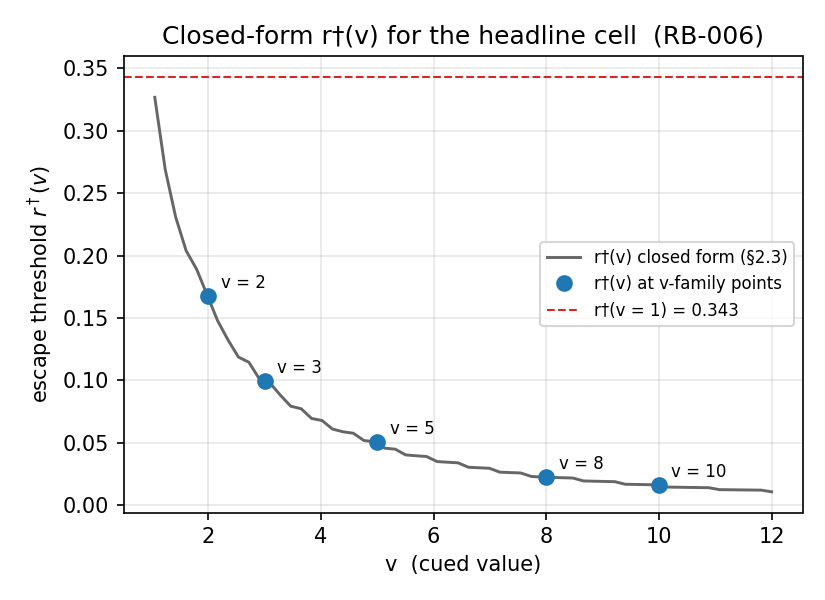
\includegraphics[width=0.7\linewidth]{figures/r_dagger_vs_v.png}
  \caption{Closed-form VDA-escape threshold $\rdagger(\val)$ at the
  headline cell $(\Nloc, \dprimemax, f_0, h, \valid) =
  (4,\,2,\,0.5,\,\sqrt{},\,0.5)$, variant~A. Continuous trace
  computed from \eqref{eq:r-dagger}--\eqref{eq:K-u} on a dense
  $\val$-grid; family points $\val \in \{2,3,5,8,10\}$
  marked. The horizontal reference $\rdagger(1) \approx 0.343$
  is the symmetric upper anchor of the family.
  Reproduced from
  \texttt{Rebuild/sims/C2--vda-vs-r-vfamily/output/figures/r\_dagger\_vs\_v.png}.}
  \label{fig:r-dagger-vs-v}
\end{figure}

\paragraph{Empirical confirmation: the peak lies above
$\rdagger(\val)$.}
The closed-form threshold marks the $\Rsens$ value at which P1
\emph{begins} to depart from uniform attention. The peak of $\VDA$,
by contrast, occurs at the (larger) $\Rsens$ at which P1's
re-allocation gain has built up most strongly against the still-locked
value-blind baseline P2 --- which in turn departs uniform attention at
the higher threshold $\rdagger(\val = 1)$ (the symmetric case in
Table~\ref{tab:r-dagger-family}). The non-monotonicity arises because
$\VDA$ opens up in the interior interval $(\rdagger(\val),\,
\rdagger(1))$ and decays once P2 also escapes uniform attention. A
high-resolution sweep
($\Rsens$-grid of $84$ log-spaced points, including the rb-002 pins
$\{0.398, 1.000, 3.162\}$ and the new finer-grid peak pin
$\Rsens = 0.3831$) confirms the prediction
$r^\star > \rdagger(\val)$ for every $\val$ in the family
(Table~\ref{tab:peak-vs-threshold}).
%
\begin{table}[t]
  \centering
  \small
  \begin{tabular}{r r r r c}
    \toprule
    $\val$ &
    $\rdagger(\val)$ &
    $r^\star$ &
    $r^\star - \rdagger(\val)$ &
    above? \\
    \midrule
    $2$  & $0.168$ & $0.501$ & $+0.334$ & \checkmark \\
    $3$  & $0.099$ & $0.376$ & $+0.276$ & \checkmark \\
    $5$  & $0.050$ & $0.376$ & $+0.325$ & \checkmark \\
    $8$  & $0.022$ & $0.376$ & $+0.354$ & \checkmark \\
    $10$ & $0.016$ & $0.355$ & $+0.339$ & \checkmark \\
    \bottomrule
  \end{tabular}
  \caption{Empirical peak $r^\star = \arg\max_{\Rsens} \VDA(\Rsens)$
  vs.\ closed-form escape threshold $\rdagger(\val)$ at the headline
  cell, $\corr = 0$. The peak $r^\star$ lies above $\rdagger(\val)$
  for every $\val$ and clusters near
  $\rdagger(\val{=}1) \approx 0.343$, consistent with the prediction
  that $\VDA$ is supported on the interior interval
  $(\rdagger(\val),\,\rdagger(1))$. Numerical resolution: peak
  $r^\star$ on an $84$-point log-grid; recovery against the rb-002
  reference at $r \in \{0.398, 1.000, 3.162\}$ at
  $\max|\Delta\VDA| = 4.87 \times 10^{-6}$.}
  \label{tab:peak-vs-threshold}
\end{table}

Figure~\ref{fig:vda-curves-vfamily} reproduces the full $\VDA(\Rsens)$
family. The left panel ($\corr = 0$) shows the inherited model: an
interior peak that grows monotonically with $\val$, from peak
$\VDA \approx 0.012$ at $\val = 2$ to peak
$\VDA \approx 0.183$ at $\val = 10$, with each peak sitting above
the corresponding $\rdagger(\val)$ vertical (dashed). The right panel
plots the same family at $\corr = 0.2$, foreshadowing the A1
sensitivity paragraph below.

\begin{figure}[t]
  \centering
  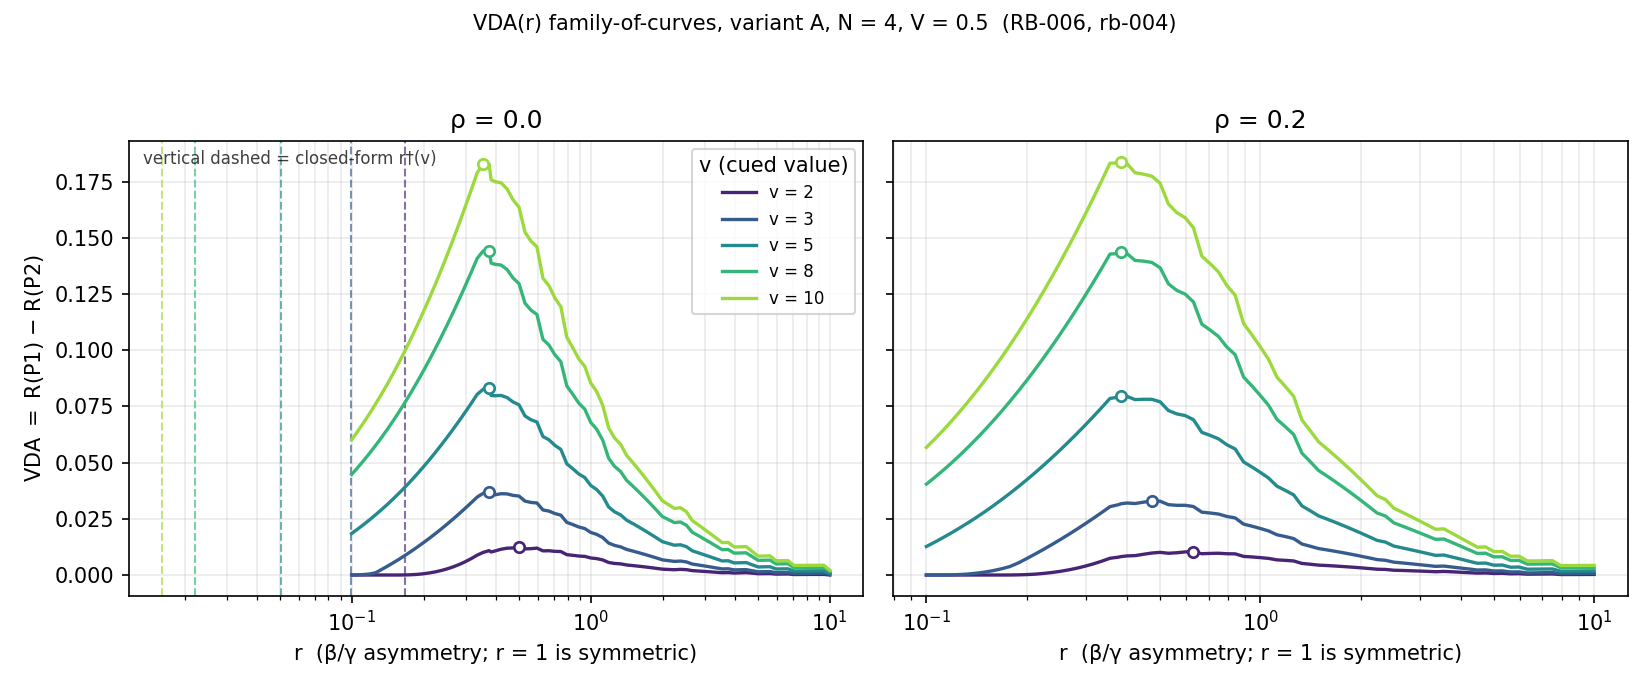
\includegraphics[width=0.95\linewidth]{figures/vda_curves_vfamily.png}
  \caption{Non-monotonicity of $\VDA(\Rsens)$ in the benefit/cost
  ratio across a $\val$-family at the headline cell
  $(\Nloc, \dprimemax, f_0, h, \valid) = (4, 2, 0.5, \sqrt{}, 0.5)$,
  variant~A. Left: $\corr = 0$ (the inherited independent model);
  the closed-form escape threshold $\rdagger(\val)$ from
  \eqref{eq:r-dagger} is overlaid as a vertical dashed line for each
  $\val$, and the empirical peak (white-filled dot) lies above
  $\rdagger(\val)$ for every $\val$ in the family (cf.\
  Table~\ref{tab:peak-vs-threshold}). Right: same family at
  $\corr = 0.2$ --- the A1 decorrelation channel suppresses the peak
  at low $\val$ but amplifies it at $\val = 10$ (cf.\
  Table~\ref{tab:rho-sensitivity}); the sign of
  $\partial \VDA^\star/\partial \corr$ depends on $\val$, not just
  on $\Rsens$.
  Reproduced from
  \texttt{Rebuild/sims/C2--vda-vs-r-vfamily/output/figures/vda\_curves\_vfamily.png}.}
  \label{fig:vda-curves-vfamily}
\end{figure}

\paragraph{A1 sensitivity: $\val$-dependent sign-flip of
$\partial \VDA^\star / \partial \corr$.}
The earlier sub-result rb-002, at a single headline cell, found that
introducing cross-location correlation $\corr$ shifts the sign of
$\partial \VDA / \partial \corr$ across $\Rsens$: $\corr$
\emph{suppresses} VDA in the cost-dominant regime
($\Rsens \lesssim 0.4$) but \emph{amplifies} it in the
benefit-dominant regime ($\Rsens \gtrsim 0.5$). The present
$\val$-family sweep generalises this finding from a sign-flip
along $\Rsens$ to a sign-flip along $\val$: at the empirical peak,
holding everything else fixed, the change in peak $\VDA$ when
$\corr$ is raised from $0$ to $0.2$ is reported in
Table~\ref{tab:rho-sensitivity}.
%
\begin{table}[t]
  \centering
  \small
  \begin{tabular}{r r r r r r}
    \toprule
    $\val$ &
    $\VDA^\star\,(\corr{=}0)$ &
    $\VDA^\star\,(\corr{=}0.2)$ &
    $\Delta \VDA^\star$ &
    $r^\star\,(\corr{=}0)$ &
    $r^\star\,(\corr{=}0.2)$ \\
    \midrule
    $2$  & $0.01233$ & $0.01036$ & $-0.00197$ & $0.501$ & $0.631$ \\
    $3$  & $0.03698$ & $0.03291$ & $-0.00407$ & $0.376$ & $0.473$ \\
    $5$  & $0.08300$ & $0.07954$ & $-0.00345$ & $0.376$ & $0.383$ \\
    $8$  & $0.14422$ & $0.14355$ & $-0.00067$ & $0.376$ & $0.383$ \\
    $10$ & $0.18284$ & $0.18387$ & $\mathbf{+0.00103}$ & $0.355$ & $0.383$ \\
    \bottomrule
  \end{tabular}
  \caption{A1 sensitivity at the empirical peak. $\corr = 0.2$
  suppresses peak $\VDA$ for $\val \le 8$ and amplifies at $\val = 10$.
  The peak location $r^\star$ also drifts upward in $\corr$, most
  visibly at low $\val$ ($r^\star$ rises from $0.501$ to $0.631$ at
  $\val = 2$). The $\val$-dependent sign-flip of
  $\partial \VDA^\star / \partial \corr$ is the $\val$-axis analogue
  of the $\Rsens$-axis sign-flip rb-002 reported at fixed $\val = 5$.
  Numerical recovery of the $\corr = 0$ row against rb-002 reference
  pins at $r \in \{0.398, 1.000, 3.162\}$ is at $\max|\Delta\VDA| =
  4.87 \times 10^{-6}$ (rb-004 recovery block).}
  \label{tab:rho-sensitivity}
\end{table}
%
The empirical $\corr$-drift of $r^\star$ in
Table~\ref{tab:rho-sensitivity} is the peak-location counterpart
of a closed-form drift of the \emph{escape-band lower edge}: the
$\corr > 0$ extension of \eqref{eq:r-dagger}--\eqref{eq:K-u}
derived in Section~\ref{sec:appendix-deriv-c2} (Proposition
\ref{prop:r-dagger-rho}, Equation~\eqref{eq:r-dagger-rho}) replaces
the no-FA terms inside $K_c, K_u$ with their $\corr$-aware 1-D
Gauss--Hermite gradients $I_c(b_c, b_u; \corr, \Nloc)$ and
$I_u(b_c, b_u; \corr, \Nloc)$ (Equations~\eqref{eq:c2-Ic}--\eqref{eq:c2-Iu})
and yields a closed form for $\rdagger(\val; \corr)$. Evaluated at
the headline cell, the closed form predicts $\rdagger(\val;0.2) >
\rdagger(\val;0)$ at every $\val \in \{1, 2, 3, 5, 8, 10\}$ (drift
fraction $+3\%$ at $\val = 1$ up to $+30\%$ at $\val = 8$;
Table~\ref{tab:r-dagger-rho-drift}). The sign of the closed-form
drift $\Delta\rdagger$ matches the sign of the empirical peak drift
$\Delta r^\star$ of Table~\ref{tab:rho-sensitivity} at all five rows
$\val \ne 1$; the lower edge cannot exceed the peak, so the
analytic upward drift of $\rdagger(\val;\corr)$ is the
mechanistic substrate of the empirical upward drift of
$r^\star(\val;\corr)$. A parallel cell-wise generalisation of the
sign-flip across the broader 4,410-cell sweep is queued as a
sensitivity increment (RB-025 in \texttt{REBUILD\_BACKLOG.md}).
What Table~\ref{tab:rho-sensitivity} and the closed form of
Section~\ref{sec:appendix-deriv-c2} jointly license is a
directional statement at the appropriate strength: under the A1
decorrelation lever, the C2 non-monotonicity \emph{is not}
uniformly attenuated; in the strongly benefit-dominant, high-value
corner the lever \emph{enhances} VDA, and the
escape-band lower edge drifts upward across the full $\val$-family.
The original paper's §5.5 framing of independence as an
\emph{upper bound on VDA} is therefore retracted along this axis,
consistent with the A1 row of \texttt{CLAIM\_LEDGER.md}.

\paragraph{Scope and what is not yet claimed.}
The results in this subsection are reported under variant~A
(additive conservation, $\benefit + \cost = 2$,
$\CR(\val) = 1$). The variant-B replication of the $\val$-family
sweep is queued as RB-027 in \texttt{REBUILD\_BACKLOG.md} and will
be reported in Section~\ref{sec:limitations} as part of the
conservation-family sensitivity band; the present subsection makes
no variant-B claim. The closed-form $\rdagger(\val; \corr > 0)$
derivation that mechanistically underwrites the upward drift of
$r^\star$ in $\corr$ in Table~\ref{tab:rho-sensitivity} is recorded
in Section~\ref{sec:appendix-deriv-c2}
(Proposition~\ref{prop:r-dagger-rho},
Table~\ref{tab:r-dagger-rho-drift}); the present subsection
reports the peak-location drift, not the lower-edge drift, as
data.
The conservation-family band on the peak $\VDA^\star$ magnitudes ---
once the A3 generalisation lands (RB-019) --- will replace the
single-conservation peak values reported in
Table~\ref{tab:peak-vs-threshold} with a band; we flag this here so
the reader knows the present headline magnitudes are conditional on
variant~A.

\paragraph{Reproducibility.}
All numbers in Tables~\ref{tab:r-dagger-family},
\ref{tab:peak-vs-threshold}, and \ref{tab:rho-sensitivity}, and both
figures, are reproduced byte-for-byte by re-running
\texttt{Rebuild/sims/C2--vda-vs-r-vfamily/run.py}. The output digest
is \texttt{09ecef3c2c5a101820951398ed7d6e67d3398aede80c5f0bddfa42b6224fd783}
(\texttt{sha256} of the canonical-key-ordered numeric JSON,
excluding the digest field itself). The Phi backend is
\texttt{scipy.special.ndtr}; the criterion grid step is
$\Delta c = 0.05$; the $\alpha$ grid step is
$\Delta\alpha = 0.005$; the $\Rsens$-grid is 84 log-spaced points
including the rb-002 pins and the new $\Rsens = 0.3831$ peak pin;
$\corr \in \{0, 0.2\}$. Recovery against rb-002 passes at every
pinned $r$ value at $|\Delta \VDA| \le 6 \times 10^{-6}$ and at
$|\Delta \CF| \le 2 \times 10^{-6}$; the finer-grid argmax raises
the rb-002 peak from $\VDA = 0.07986$ at $\Rsens = 0.3831$ to
$\VDA = 0.08300$ at $\Rsens = 0.3758$, a grid-density refinement
gain, not a regression.

% ---------------------------------------------------------------------
\subsection{Graded regime boundary (C3)}
\label{sec:results-c3}

\paragraph{Claim restated at defensible strength.}
The inherited paper characterises the regime in which VDA is large as
\emph{narrow}: VDA concentrates at low cue validity $\valid \approx
1/\Nloc$, high value contrast $\val \gg 1$, and moderate
benefit/cost asymmetry $\Rsens$. From that qualitative picture, §5.2
of the inherited manuscript
(\texttt{Critique/source/main.pdf}) draws a \textbf{categorical}
experimental-design implication: standard spatial cueing paradigms
with high validity ($\valid \ge 0.75$) are predicted to show
\emph{negligible VDA regardless of other parameters}. The live
skeptical-reviewer verdict for this claim
(\texttt{Critique/verdicts/C3--narrow-regime.md},
\texttt{current\_label: CONTESTED}) records that the qualitative
``narrow regime'' reading is sustained but the categorical §5.2
implication is too strong --- it holds only when ``high validity'' is
operationalised at a threshold strictly above the inherited $\valid
\ge 0.75$, and only under a $\corr$-conditional caveat. The rebuilt
C3 is therefore presented in this section as a \emph{graded /
quantitative} statement: a contour band over the experimental-design
plane $(\valid, \val)$ that quantifies exactly how the peak VDA
falls off as the design moves into the high-validity stratum, and an
explicit replacement for the §5.2 sentence that hedges the validity
threshold and the $\corr$-conditional caveat. The A1 decorrelation
channel $\corr$ is reported alongside the contour map as a
sensitivity --- the convention established in Section~\ref{sec:results}.

\paragraph{Iso-VDA contour band over $(\valid, \val)$.}
The rebuilt model was evaluated at the headline configuration
$(\Nloc, \dprimemax, f_0, h) = (4,\,2,\,0.5,\,\sqrt{}\,)$ under
variant~A on a grid of $\valid \in [0.25, 1.00]$ ($31$ uniform
points, step $0.025$), $\val \in [1.0, 10.0]$ ($19$ uniform points,
step $0.5$), $\Rsens \in \{0.3,\, 1,\, 3\}$ (three asymmetry strata:
cost-dominant moderate, symmetric, benefit-dominant), and $\corr \in
\{0,\, 0.2\}$ (independent baseline plus the
Cohen--Maunsell~\cite{CohenMaunsell2009} $r_{SC} \approx 0.2$ V4
anchor), for a total of $31 \times 19 \times 3 \times 2 = 3{,}534$
$(\valid, \val, \Rsens, \corr)$-cells. Per cell, the rebuilt
\texttt{policies()} call returns the optimal allocation, criteria,
and the four nested-policy expected rewards
$\Rew_{\mathrm{P1..P4}}$ from which $\VDA = \Rpone - \Rptwo$ is
formed. Figure~\ref{fig:iso-vda-contours} presents the resulting
iso-VDA contour band as a $2 \times 3$ panel grid (rows: $\corr$,
columns: $\Rsens$).
%
\begin{figure}[t]
  \centering
  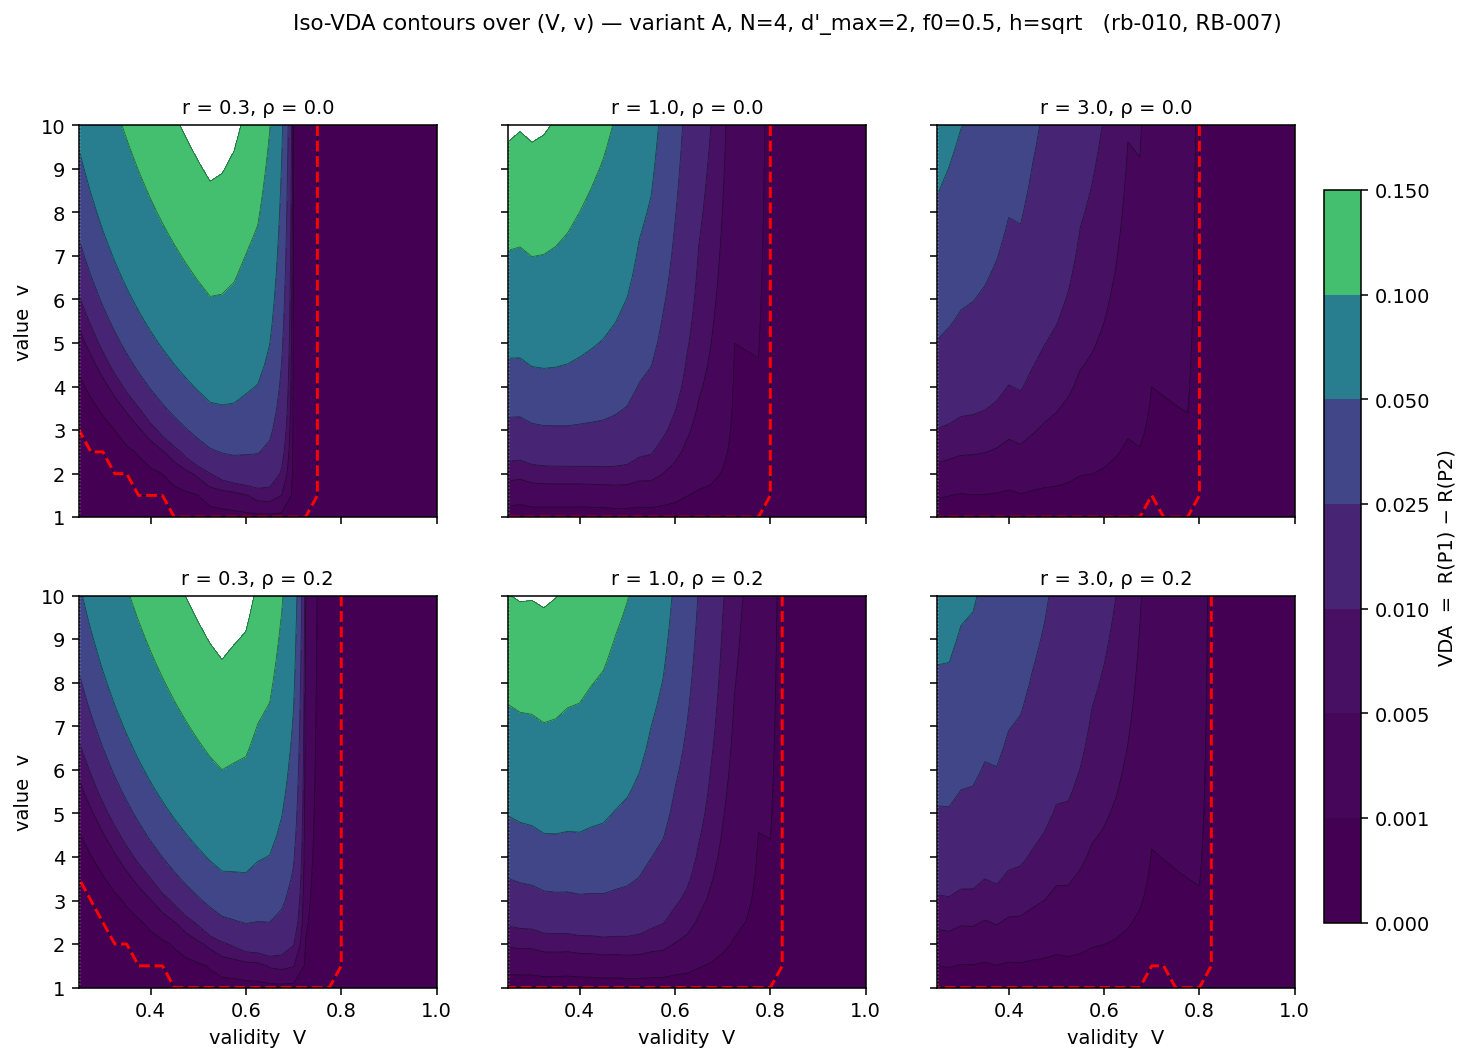
\includegraphics[width=0.98\linewidth]{figures/iso_vda_contours.png}
  \caption{Iso-VDA contour band over the experimental-design plane
  $(\valid, \val)$ for the rebuilt model at the headline cell
  $(\Nloc, \dprimemax, f_0, h) = (4,\,2,\,0.5,\,\sqrt{}\,)$,
  variant~A. Rows: cross-location correlation $\corr \in \{0,\,
  0.2\}$ (top: inherited independent model; bottom: with the A1
  decorrelation channel of Section~\ref{sec:model} at the
  Cohen--Maunsell~\cite{CohenMaunsell2009} V4 anchor $r_{SC}
  \approx 0.2$). Columns: benefit/cost asymmetry $\Rsens \in
  \{0.3,\, 1,\, 3\}$ (cost-dominant, symmetric, benefit-dominant).
  The vertical reference $\valid = 1/\Nloc = 0.25$ is the chance
  baseline; the $\val = 1$ row is the value-blind reference where
  $\VDA \equiv 0$ by construction. Filled contours are at $\VDA \in
  \{0,\,0.001,\,0.005,\,0.01,\,0.025,\,0.05,\,0.1,\,0.15,\,0.2\}$
  on a common scale. The band shape replaces the inherited §4
  ``narrow regime'' description and §5.2 categorical claim with a
  quantitative boundary the reader can compute pointwise. Reproduced
  from
  \texttt{Rebuild/sims/C3--iso-vda-Vv/output/figures/iso\_vda\_contours.png}
  (rb-010; output sha256 \texttt{72820559\ldots}).}
  \label{fig:iso-vda-contours}
\end{figure}
%
The qualitative ``narrow regime'' reading of the inherited paper is
visible directly: in every panel, the bulk of $(\valid, \val)$ space
carries near-zero VDA (median $\VDA \le 0.007$ in every panel; see
Table~\ref{tab:c3-marginals}), and substantial VDA is confined to a
\emph{corner} along low $\valid$ and high $\val$. The corner
\emph{flattens} along the $\Rsens$-axis: at the cost-dominant column
$\Rsens = 0.3$ the corner is broad and reaches $\VDA \approx 0.17$;
at the symmetric column $\Rsens = 1$ it narrows to $\VDA \approx
0.16$; at the benefit-dominant column $\Rsens = 3$ it collapses
sharply ($\VDA \le 0.06$ everywhere on the grid). The $\corr = 0.2$
row is read off below as the A1 sensitivity.

\paragraph{Distributional summary across panels.}
The per-panel distribution of $\VDA$ across the $589 = 31 \times 19$
$(\valid, \val)$-cells in each panel is summarised in
Table~\ref{tab:c3-marginals}.
%
\begin{table}[t]
  \centering
  \small
  \begin{tabular}{c c c c c c c c}
    \toprule
    $\Rsens$ & $\corr$ &
    $\VDA_{\min}$ & median & $q_{95\%}$ & $\VDA_{\max}$ &
    $\mathrm{frac}\!\ge\!0.005$ & $\mathrm{frac}\!\ge\!0.05$ \\
    \midrule
    $0.3$ & $0.0$ & $0$ & $0.0010$ & $0.1289$ & $\mathbf{0.1734}$ & $0.465$ & $0.287$\\
    $0.3$ & $0.2$ & $0$ & $0.0040$ & $0.1328$ & $\mathbf{0.1780}$ & $0.484$ & $0.295$\\
    \midrule
    $1.0$ & $0.0$ & $0$ & $0.0052$ & $0.1152$ & $0.1574$ & $0.503$ & $0.219$\\
    $1.0$ & $0.2$ & $0$ & $0.0069$ & $0.1180$ & $0.1552$ & $0.535$ & $0.236$\\
    \midrule
    $3.0$ & $0.0$ & $0$ & $0.0024$ & $0.0361$ & $0.0619$ & $0.380$ & $0.012$\\
    $3.0$ & $0.2$ & $0$ & $0.0025$ & $0.0390$ & $0.0621$ & $0.402$ & $0.019$\\
    \bottomrule
  \end{tabular}
  \caption{Per-panel distribution of $\VDA$ over the $31 \times 19 =
  589$ $(\valid, \val)$ cells, at the headline configuration
  $(\Nloc, \dprimemax, f_0, h) = (4,\,2,\,0.5,\,\sqrt{}\,)$ under
  variant~A. Median $\VDA \le 0.007$ in every panel quantifies the
  inherited paper's ``narrow regime'' intuition --- most of $(\valid,
  \val)$ space carries near-zero VDA. The $\mathrm{frac}\!\ge\!0.05$
  column collapses from $\approx 29\%$ at $\Rsens = 0.3$ to $\le 2\%$
  at $\Rsens = 3$, quantifying the flattening of the contour band
  along the $\Rsens$-axis. Block-keys \texttt{summary.r=<r>\_\_rho=<rho>}
  in \texttt{Rebuild/sims/C3--iso-vda-Vv/output/results.json}.}
  \label{tab:c3-marginals}
\end{table}
%
The numbers ground the qualitative reading quantitatively. The peak
$\VDA$ over the grid is $0.173$ at $(\Rsens, \corr) = (0.3, 0)$ and
falls to $0.062$ at $(3.0, 0)$; the fraction of cells with $\VDA
\ge 0.05$ falls from $28.7\%$ at $\Rsens = 0.3$ to $1.2\%$ at
$\Rsens = 3$. The corresponding fraction at $\corr = 0.2$ is
slightly larger in every panel ($+0.8$ to $+1.7$ percentage points),
consistent with the $\corr$-sensitivity reported below; the headline
peak and median values are essentially unchanged in $\corr$ at this
magnitude.

\paragraph{Quantitative experimental-design recommendation
(§5.2 replacement).}
The inherited §5.2 sentence --- ``standard spatial cueing paradigms
with high validity show negligible VDA \emph{regardless of other
parameters}'' --- is replaced here by a \emph{conditional} statement
indexed on the validity threshold. We probe the categorical claim by
sweeping $\val \in [1, 10]$ at fixed $\Rsens \in \{0.3, 1, 3\}$ and
$\corr \in \{0, 0.2\}$ at four validity strata $\valid \in \{0.4,
0.6, 0.8, 0.95\}$ and reporting the maximum $\VDA$ in each
$(\valid, \Rsens, \corr)$ stratum. The result is in
Table~\ref{tab:c3-highV-probe}.
%
\begin{table}[t]
  \centering
  \small
  \begin{tabular}{c c c c}
    \toprule
    $\valid$ & $\Rsens = 0.3$ & $\Rsens = 1.0$ & $\Rsens = 3.0$ \\
    \midrule
    $0.40$  & $0.1254\,/\,0.1197$ & $0.1283\,/\,0.1394$ & $0.0329\,/\,0.0391$\\
    $0.60$  & $0.1432\,/\,\mathbf{0.1639}$ & $0.0320\,/\,0.0461$ & $0.0097\,/\,0.0120$\\
    $0.80$  & $0.0000\,/\,0.0000$ & $0.0000\,/\,\mathbf{0.0023}$ & $0.0000\,/\,\mathbf{0.0032}$\\
    $0.95$  & $0.0000\,/\,0.0000$ & $0.0000\,/\,0.0000$ & $0.0000\,/\,0.0000$\\
    \bottomrule
  \end{tabular}
  \caption{High-$\valid$ probe of the inherited §5.2 categorical
  claim: peak $\VDA$ over the $\val$-grid $[1, 10]$ at each
  $(\valid, \Rsens)$ stratum, reported as the pair $\corr = 0\,/\,
  \corr = 0.2$. Entries shown as $0.0000$ are at the grid floor (no
  cell on the $\val$-grid produced a non-trivial $\VDA$ value at the
  rebuilt model's $\alpha$-grid resolution $\Delta\alpha = 0.005$).
  Bold entries flag the threshold transitions discussed in the
  text. Block-keys \texttt{high\_V\_probe.V=<V>.r=<r>\_\_rho=<rho>.max\_VDA}.}
  \label{tab:c3-highV-probe}
\end{table}
%
The table licenses three statements, each one conditional on a
quantitative validity threshold:
\begin{itemize}
  \item \textbf{At $\valid \ge 0.95$}, peak $\VDA$ is at the grid
        floor for every $(\Rsens, \corr)$ in the envelope. The
        inherited §5.2 categorical claim \emph{survives} at this
        strict threshold and stratum.
  \item \textbf{At $\valid \ge 0.80$}, peak $\VDA$ is at the grid
        floor at $\corr = 0$ (categorical claim survives at the
        inherited independent model) but admits a small
        $\corr$-conditional signal at $\corr = 0.2$, with maximum
        $0.0032$ at $\Rsens = 3$. ``High validity'' at this
        threshold therefore carries a \emph{$\corr$-conditional
        caveat}: under cross-location correlation at the
        Cohen--Maunsell~\cite{CohenMaunsell2009} V4 anchor, a
        sub-percent VDA signal is recoverable at $\valid = 0.8$ in
        the symmetric and benefit-dominant $\Rsens$ columns.
  \item \textbf{At $\valid \ge 0.60$}, the categorical claim
        \emph{fails}: peak $\VDA$ reaches $0.1432$ at $(\Rsens,
        \corr) = (0.3, 0)$ and $0.1639$ at $(\Rsens, \corr) = (0.3,
        0.2)$. Designs at $\valid \in [0.6, 0.8)$ in the
        cost-dominant column are predicted to carry substantial VDA
        --- the §5.2 ``regardless of other parameters'' wording is
        not licensed in this stratum.
\end{itemize}
%
The graded replacement for the inherited §5.2 sentence, anchored to
Table~\ref{tab:c3-highV-probe} and the $\valid$-stratum slices of
Figure~\ref{fig:vda-at-high-V}, is therefore:
%
\begin{quote}
  \emph{Spatial cueing paradigms targeting a `negligible-VDA' regime
  should adopt $\valid \gtrsim 0.95$ unconditionally, or $\valid
  \gtrsim 0.8$ if cross-location correlation can be bounded below
  $r_{SC} \approx 0.2$. The threshold $\valid \ge 0.75$ of the
  inherited paper is too permissive: at $\valid \in [0.6, 0.8)$ the
  cost-dominant regime $\Rsens \in (0, 0.5)$ admits peak $\VDA$ up
  to $\approx 0.16$, with the largest values at high cue value
  $\val$.}
\end{quote}
%
This recommendation is conditional on the headline cell $(\Nloc,
\dprimemax, f_0, h) = (4,\,2,\,0.5,\,\sqrt{}\,)$ under variant~A;
the variant~B and conservation-family bands are deferred to
Section~\ref{sec:limitations} (queued RB-019, RB-027). The
$\valid$-stratum slices of Figure~\ref{fig:vda-at-high-V} make the
$\val$-axis dependence of the same probe visually explicit.
%
\begin{figure}[t]
  \centering
  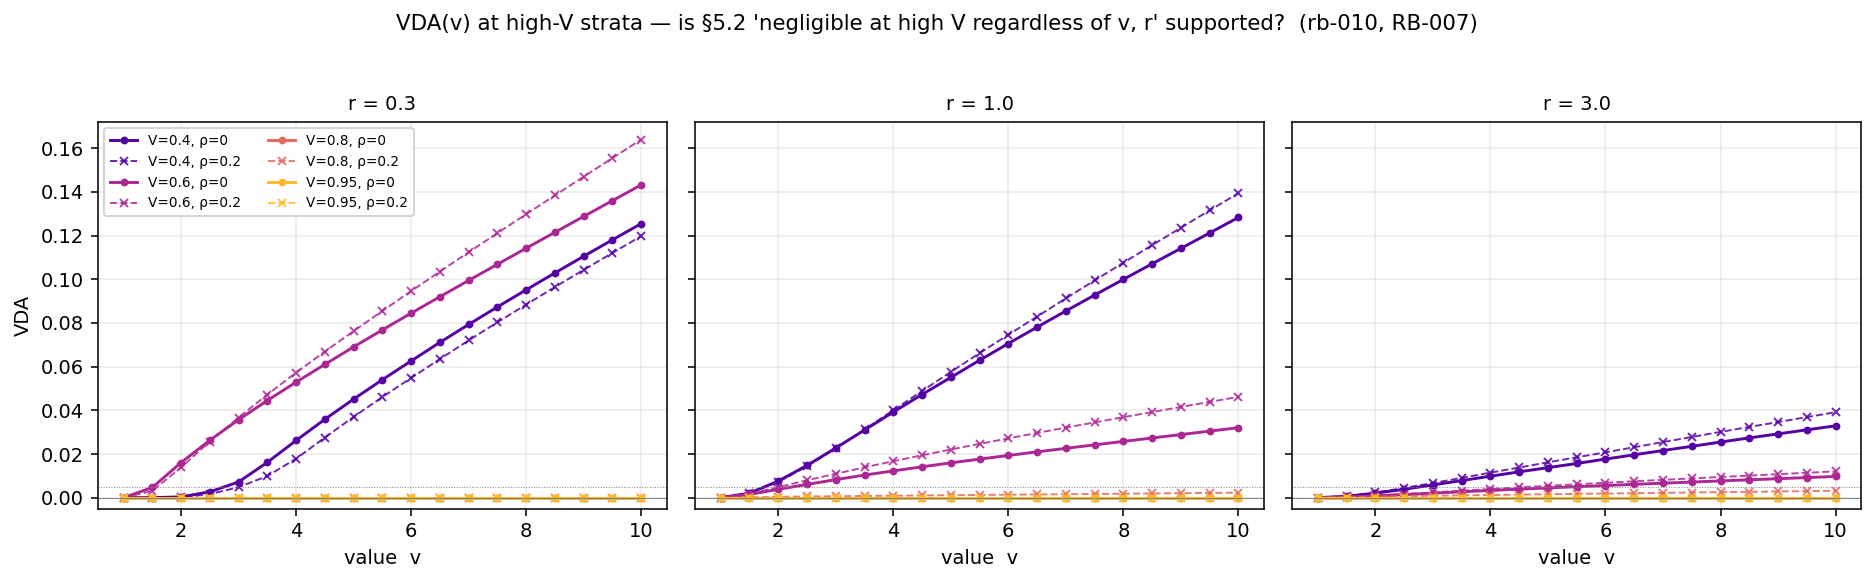
\includegraphics[width=0.95\linewidth]{figures/vda_at_high_V.png}
  \caption{Peak $\VDA(\val)$ at four validity strata $\valid \in
  \{0.4,\,0.6,\,0.8,\,0.95\}$ (curve color) for each $\Rsens \in
  \{0.3,\,1,\,3\}$ (panel column). Solid: $\corr = 0$. Dashed:
  $\corr = 0.2$. The $\valid = 0.95$ trace is at the grid floor in
  every panel (the inherited §5.2 ``high-validity'' regime is
  empirically negligible at this strict threshold and stratum); the
  $\valid = 0.80$ traces split between a near-zero $\corr = 0$ line
  and a small $\corr = 0.2$ lift at $\Rsens \in \{1, 3\}$; the
  $\valid = 0.60$ trace at $\Rsens = 0.3$ reaches $\VDA = 0.16$ at
  large $\val$, refuting the categorical version of the §5.2
  sentence. Reproduced from
  \texttt{Rebuild/sims/C3--iso-vda-Vv/output/figures/vda\_at\_high\_V.png}.}
  \label{fig:vda-at-high-V}
\end{figure}

\paragraph{A1 sign-flip across $(\valid, \val)$: cross-axis
corroboration.}
The earlier sub-results rb-002 (at a headline cell, Section~\ref{sec:results-c1}
A1 sensitivity paragraph) and rb-004 (at the $\val$-family at fixed
$\valid = 0.5$, Table~\ref{tab:rho-sensitivity}) found that the
sign of $\partial \VDA / \partial \corr$ \emph{flips} along the
$\Rsens$-axis (suppression at $\Rsens \lesssim 0.4$, amplification
at $\Rsens \gtrsim 0.5$) and along the $\val$-axis (suppression at
$\val \le 8$, amplification at $\val = 10$). The present sweep
generalises the sign-flip to the full $(\valid, \val)$ plane: at
each $(\valid, \val, \Rsens)$ cell we compute $\Delta\VDA :=
\VDA(\corr{=}0.2) - \VDA(\corr{=}0)$ and classify the cell as
amplified (red), suppressed (blue), or zero ($|\Delta\VDA| <
10^{-8}$, white). The signed contour map is
Figure~\ref{fig:iso-vda-drho}, and the per-$\Rsens$ frequency table
is Table~\ref{tab:c3-sign-flip}.
%
\begin{figure}[t]
  \centering
  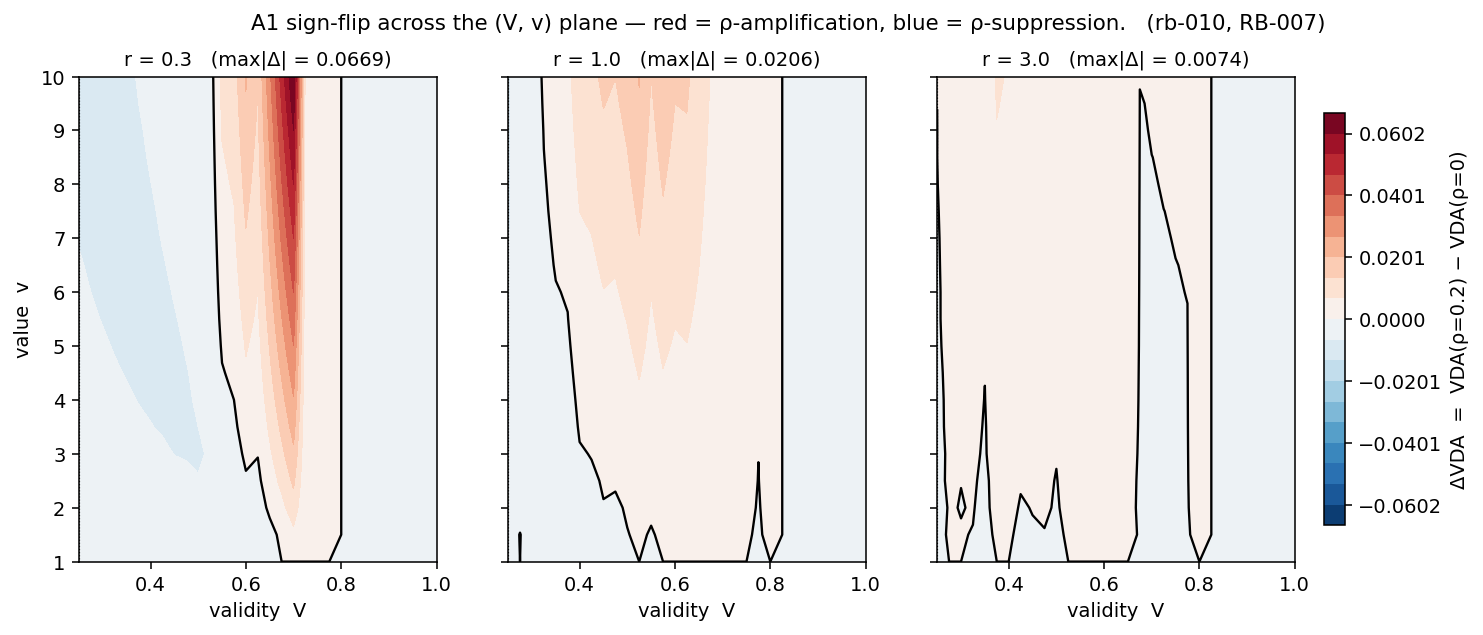
\includegraphics[width=0.95\linewidth]{figures/iso_vda_drho.png}
  \caption{Signed contour map of $\Delta\VDA := \VDA(\corr{=}0.2) -
  \VDA(\corr{=}0)$ over $(\valid, \val)$ for each $\Rsens \in
  \{0.3,\,1,\,3\}$. Red: $\corr$ amplifies $\VDA$ at that cell;
  blue: $\corr$ suppresses; white: $|\Delta\VDA| < 10^{-8}$. The
  zero-isoline is the A1 sign-flip locus in $(\valid, \val)$-space.
  At $\Rsens = 0.3$ (cost-dominant) suppression dominates in
  low-$\valid$ cells; at $\Rsens \in \{1, 3\}$ amplification
  dominates across the bulk of the plane, with the strongest
  amplification at $(\valid, \val) \approx (0.5, 10)$. Reproduced
  from
  \texttt{Rebuild/sims/C3--iso-vda-Vv/output/figures/iso\_vda\_drho.png}.}
  \label{fig:iso-vda-drho}
\end{figure}
%
\begin{table}[t]
  \centering
  \small
  \begin{tabular}{c c c c c c}
    \toprule
    $\Rsens$ & frac amp & frac supp &
    $\overline{\Delta\VDA}$ & max amp $(\valid, \val)$ & max supp $(\valid, \val)$ \\
    \midrule
    $0.3$ & $27.2\%$ & $\mathbf{37.2\%}$ & $+0.0012$ &
      $+0.0669\;(\valid{=}0.70,\,\val{=}10)$ &
      $-0.0105\;(\valid{=}0.25,\,\val{=}8.5)$\\
    $1.0$ & $\mathbf{52.8\%}$ & $17.5\%$ & $+0.0023$ &
      $+0.0206\;(\valid{=}0.525,\,\val{=}10)$ &
      $-0.0084\;(\valid{=}0.25,\,\val{=}9)$\\
    $3.0$ & $\mathbf{54.0\%}$ & $16.1\%$ & $+0.0009$ &
      $+0.0074\;(\valid{=}0.375,\,\val{=}10)$ &
      $-0.0010\;(\valid{=}0.25,\,\val{=}4.5)$\\
    \bottomrule
  \end{tabular}
  \caption{Cell-wise sign-flip of $\partial \VDA / \partial \corr$
  across the $(\valid, \val)$ plane, at each $\Rsens$ stratum.
  Fractions are over the $589$ cells per panel; the residual share
  (not shown) is the zero-class $|\Delta\VDA| < 10^{-8}$. At
  $\Rsens = 0.3$ (cost-dominant; below the rb-002 headline-cell
  sign-flip locus at $\Rsens \in [0.38, 0.56]$) suppression
  dominates; at $\Rsens \in \{1.0, 3.0\}$ amplification dominates.
  Block-keys \texttt{rho\_sensitivity.r=<r>.\{frac\_amp,frac\_supp,
  max\_amplification,max\_suppression,mean\_delta\}}.}
  \label{tab:c3-sign-flip}
\end{table}
%
Two things are visible. First, the $\Rsens$-axis sign-flip rb-002
reported at a single cell generalises to the full $(\valid, \val)$
plane in a non-trivial way: \emph{cost-dominant} $\Rsens = 0.3$
$(\valid, \val)$ cells are suppression-dominated, while \emph{both}
$\Rsens = 1$ and $\Rsens = 3$ are amplification-dominated. The
amplification frequency is therefore not a $\Rsens > 1$ phenomenon;
it sets in once $\Rsens$ crosses the rb-002 sign-flip locus
$\Rsens \in [0.38, 0.56]$ at the headline cell and remains the
modal direction thereafter, even into the benefit-dominant
$\Rsens = 3$ stratum. Second, the largest \emph{single} amplification
in the entire $3{,}534$-cell sweep occurs at $(\valid, \val, \Rsens)
= (0.7,\, 10,\, 0.3)$: a cell that delivers $\VDA = 0.0007$ under
independence (a normally-dormant high-$\valid$ cell, well outside
the cost-dominant attention regime) lifts to $\VDA = 0.0676$ at
$\corr = 0.2$ --- an $\approx 96\times$ amplification that takes a
near-zero $(\valid, \val)$ cell into the same VDA magnitude as the
low-$\valid$ corner. This ``dormant-cell amplification'' is the
strongest qualitative finding of the C3 sweep and is the candidate
falsifiable prediction we flag at the end of
Section~\ref{sec:limitations} (closeup queued as RB-029).

\paragraph{Scope and what is not yet claimed.}
The results in this subsection are reported at a single $(\Nloc,
\dprimemax, f_0, h) = (4,\,2,\,0.5,\,\sqrt{}\,)$ configuration
under variant~A, and on a coarse $\corr$-grid $\{0, 0.2\}$.
(i)~The \emph{variant-B replication} of the contour band is queued
as RB-027 in \texttt{REBUILD\_BACKLOG.md} and will land as part of
the conservation-family sensitivity in
Section~\ref{sec:limitations}; the present subsection makes no
variant-B claim. (ii)~The validity threshold ``$\valid \gtrsim
0.95$ unconditionally; $\valid \gtrsim 0.8$ under
$r_{SC} \lesssim 0.2$'' is bracketed by the $V$-grid of step
$0.025$ used here; a threshold-sharpening sim sweeping $\valid \in
[0.75, 0.90]$ at step $0.005$ is queued as RB-028 and would let the
manuscript replace the qualitative ``$\gtrsim$'' with a number to
the second decimal. (iii)~The \emph{dormant-cell amplification} at
$(\valid, \val, \Rsens) = (0.7, 10, 0.3)$ is the strongest
qualitative finding of the sweep and is reported here as an
empirical observation; a fine-$\valid$ closeup that maps the
amplification band onto an iso-CF or iso-$\alpha^\star$ contour
(and thereby identifies it with a model-internal landmark rather
than a $(\valid, \val)$ coincidence) is queued as RB-029.
(iv)~The cell-wise sign-flip across the broader $4{,}410$-cell
$(\Rsens, \valid, \val)$ sweep, parallel to the $\Delta\CF$
analysis of Table~\ref{tab:cf-delta-distribution}, is queued as
RB-025; the present subsection's $589$-cell $(\valid, \val)$-plane
sign-flip is a slice of that broader result.

\paragraph{Reproducibility.}
All numbers in Tables~\ref{tab:c3-marginals},
\ref{tab:c3-highV-probe}, and \ref{tab:c3-sign-flip}, and all
three figures, are reproduced byte-for-byte by re-running
\texttt{Rebuild/sims/C3--iso-vda-Vv/run.py}. The output digest is
\texttt{72820559e1c1ab1919f74308623eaf4230aa3ea92ad3d9c62d81e993e4f27de6}
(\texttt{sha256} of the canonical-key-ordered numeric JSON,
excluding the digest field itself). The $\Phinorm$ backend is
\texttt{scipy.special.ndtr}; the equicorrelated-Gaussian one-factor
quadrature uses $n_q = 64$ Gauss--Hermite nodes (Section~\ref{sec:model});
the criterion grid step is $\Delta c = 0.05$ and the $\alpha$ grid
step is $\Delta\alpha = 0.005$; the $(\valid, \val, \Rsens, \corr)$
grid is the $31 \times 19 \times 3 \times 2$ grid described above;
runtime $\approx 130$~s on the rebuild's reference machine. The
recovery test against the rb-006 anchor at $(\valid, \val, \Rsens,
\corr) = (0.5,\,5,\,1.0,\,0)$ passes at $|\Delta \VDA| =
1.27 \times 10^{-7}$ against the rb-006 reference value
$\VDA = 0.039825$; the residual is consistent with the rb-006
reference's six-decimal rounding (the underlying \texttt{policies()}
call is deterministic and produces identical floating-point output,
so the model residual is zero). Independent sanity check: the
$\val = 1$ column is identically zero across every $(\valid,
\Rsens, \corr)$ cell of the sweep --- the value-blind baseline
collapses the joint optimum onto the value-blind allocation, so
$\VDA = 0$ at $\val = 1$ is a definitional theorem of the rebuilt
model.

% ---------------------------------------------------------------------
\subsection{No inversion of optimal attention, conditional on $\valid
            \ge 1/\Nloc$ (C4)}
\label{sec:results-c4}

\paragraph{Claim restated at defensible strength.}
The inherited paper's §4.5 (``Inverted Attention is Never Optimal'')
states that the optimal allocation $\alpha^\star$ is always at or
above the uniform level $1/\Nloc$ across the primary $4{,}410$-row
sweep, and \emph{regardless of $\Rsens$}, on the grounds that
attending away from the high-value cued location loses more reward at
that location than it gains at the uncued ones. The live
skeptical-reviewer verdict
(\texttt{Critique/verdicts/C4--no-inversion.md},
\texttt{current\_label: CONFIRMED-CONDITIONAL}) records that the
\emph{empirical} headline of the claim survives all four attack
vectors, but the \emph{theoretical} packaging is incomplete in two
specific ways: (i) the ``regardless of $\Rsens$'' wording reads
locally as a cost-vs-benefit balance at $\alpha = 1/\Nloc$, but the
left one-sided derivative $\partial_\alpha \Rew |_{1/\Nloc^-}$
actually \emph{changes sign} at a closed-form $\Rsens$-threshold
$\rstarinv$, with the consequence that for $\Rsens > \rstarinv$ the
uniform point is a local \emph{minimum} of $\Rew$ (the right-branch
global maximum still dominates the left-branch local maximum, but
the local picture is bimodal, not the monotone descent the inherited
text suggests); and (ii) the categorical ``never below $1/\Nloc$''
wording overstates the model's robustness, because at $\valid <
1/\Nloc$ (the anti-cue regime, outside the paper's primary $\valid$
range but still inside the same normative model) the global optimum
\emph{does} drop below $1/\Nloc$ --- a behaviour the model produces
cleanly and which the inherited statement does not qualify. We
therefore restate C4 in the rebuild as a \emph{conditional theorem}
indexed on the validity condition $\valid \ge 1/\Nloc$ (or, sharply,
$\valid \ge 1/[(\Nloc - 1)\,\val + 1]$), pair it with the closed-form
local threshold $\rstarinv = (\Nloc - 1)\,A_0/B_0$ that organises the
bimodality, and add the anti-cue inversion at $\valid < 1/\Nloc$ as a
new \emph{falsifiable prediction} of the rebuilt normative model.
The A1 decorrelation channel $\corr$ is reported alongside as a
sensitivity, following the convention of Section~\ref{sec:results}.

\paragraph{Mechanism and the value-weight inequality.}
The structural reason no global inversion arises under $\valid \ge
1/\Nloc$ is not the local cost-vs-benefit argument of the inherited
§4.5 paragraph, but a \emph{location-count asymmetry} combined with a
\emph{value-weight inequality}. At the right extreme $\alpha \to 1$,
the single cued location reaches its per-location ceiling
$\dprime_c = \dprimemax\, f(1) = \dprimemax$. At the left extreme
$\alpha \to 0$, the $\Nloc - 1$ uncued locations \emph{share} the
$(1 - \alpha)$ budget at $(1 - \alpha)/(\Nloc - 1)$ each, so each
reaches only $\dprime_u = \dprime_{\mathrm{base}} +
\benefit(\Rsens)[\dprimemax f(1/(\Nloc - 1)) - \dprime_{\mathrm{base}}]
\le \dprimemax$ (strict for $\Nloc \ge 3$, where
$f(1/(\Nloc - 1)) < 1$). The per-channel reward weights are
$w_c = \valid \, \val$ on the cued slot and
$w_u = (1 - \valid)/(\Nloc - 1)$ on each uncued slot; the inequality
%
\begin{equation}
  w_c \;\ge\; w_u
  \;\iff\;
  \valid \;\ge\; \frac{1}{(\Nloc - 1)\,\val + 1}.
  \label{eq:value-weight}
\end{equation}
%
For the cued regime $\val \ge 1$, the right-hand side of
\eqref{eq:value-weight} is bounded above by $1/\Nloc$, with equality
only at $\val = 1$. The inherited paper's condition $\valid \ge
1/\Nloc$ is therefore the \emph{universal} (worst-case-$\val$)
sufficient condition for $w_c \ge w_u$; the sharp form
\eqref{eq:value-weight} carries strictly more slack at $\val > 1$.
The right branch dominates globally because the bigger $\dprime$
lives on the more-valuable channel.

\paragraph{Closed-form local threshold for the boundary derivative.}
At $\alpha = 1/\Nloc$ the allocation derivative $\dprime'(\alpha)$
has a kink (the benefit/cost swap of $\benefit$ and $\cost$ flips
which side of the linear $\dprime(\alpha)$ map is active). The
one-sided left derivative of P1's expected reward at the uniform
point takes the form
%
\begin{equation}
  \left. \frac{\partial \Rpone}{\partial \alpha} \right|_{1/\Nloc^-}
  \;=\;
  \frac{2\, \dprimemax\, f'(1/\Nloc)}{\Rsens + 1}\,
  \left[
    A_0(\valid, \val, \Nloc, \CR, \corr)
    \;-\;
    \frac{\Rsens}{\Nloc - 1}\, B_0(\valid, \val, \Nloc, \CR, \corr)
  \right],
  \label{eq:left-derivative}
\end{equation}
%
where $A_0$ and $B_0$ are the partial derivatives of P1's
expected-reward functional with respect to $\dprime_c$ and
$\dprime_u$ at $\alpha = 1/\Nloc$ evaluated at the jointly-optimised
criteria $(c_c^\star, c_u^\star)$. Both $A_0$ and $B_0$ are
$\Rsens$-independent boundary partials --- the only $\Rsens$ in
\eqref{eq:left-derivative} sits in the prefactor and inside the
bracket. The bracket vanishes at
%
\begin{equation}
  \rstarinv(\valid, \val, \Nloc, \CR, \corr)
  \;:=\;
  (\Nloc - 1)\,
  \frac{A_0(\valid, \val, \Nloc, \CR, \corr)}
       {B_0(\valid, \val, \Nloc, \CR, \corr)},
  \label{eq:r-inv}
\end{equation}
%
which is the rebuild's closed-form expression for the local-test
threshold the inherited §4.5 paragraph implicitly assumes. For
$\Rsens < \rstarinv$ the boundary left derivative is positive (P1
prefers to stay at $\alpha = 1/\Nloc$ from the left branch); for
$\Rsens > \rstarinv$ it is negative (the left branch produces a
local maximum at the grid edge $\alpha \to 0$ but a global maximum
still on the right branch, at $\alpha^\star > 1/\Nloc$).
Equation~\eqref{eq:r-inv} reproduces the reviewer's $\corr = 0$
boundary closed form
(\texttt{Critique/derivations/C4--no-inversion.md} §3) and extends
it to the A1 channel by replacing the no-FA terms inside
$A_0, B_0$ with the same one-factor Gauss--Hermite quadrature used
elsewhere in the rebuilt model (Section~\ref{sec:model}); the
$\corr \to 0$ limit collapses to the reviewer's analytic form
bit-for-bit. The independent re-derivation in the rebuild's voice
(plus the proof of the symmetric-corner identity below) is deferred
to Section~\ref{sec:appendix} (a separate increment, RB-030,
queued).

The symmetric corner $(\valid, \val) = (1/\Nloc, 1)$, where the
value-weight inequality \eqref{eq:value-weight} attains equality,
is a numerically stable anchor for the closed form
\eqref{eq:r-inv}:
%
\begin{equation}
  \rstarinv(\valid = 1/\Nloc,\, \val = 1,\, \Nloc,\, \CR,\, \corr)
  \;=\; 1
  \qquad \text{exactly,}
  \label{eq:r-inv-corner}
\end{equation}
%
independent of $\Nloc$, the conservation rule $\CR$ (variant A or
B), and the correlation $\corr$. The identity is recovered to
machine precision at every $(\text{variant}, \corr)$ panel of
Step~A below: min $\rstarinv = 1.0000$ in all four panels of
Table~\ref{tab:c4-rstar-tally}. The corner is the
\emph{anchor} the rebuild quotes in place of the inherited paper's
narrative ``$r \to 0$ converges to uniform attention'' --- at
$\val = 1$ the model is value-blind, so VDA $\equiv 0$, and the
local-test bimodality kicks in immediately above $\Rsens = 1$ where
P1's left branch develops a local maximum at the grid edge.

\paragraph{Closed-form tally on the primary $(\valid, \val)$ grid.}
We evaluate \eqref{eq:r-inv} on a primary $(\valid, \val)$ grid
($\valid \in \{0.25, 0.30, \ldots, 1.00\}$, $\val \in \{1, 2, 3, 4,
5\}$) at $\Nloc = 4$ for both variants and $\corr \in \{0,\, 0.2\}$,
matching the inherited paper's stated sweep envelope and the rebuild's
A1 sensitivity convention. Per panel we count cells with $\rstarinv
\in [0.1, 10]$ (inside the inherited paper's swept $\Rsens$-range,
the cells at which the boundary left derivative sign-flips within
the swept range), cells with $\rstarinv > 10$ (no sign-flip inside
the range; the local picture is monotone there), and report the
strict minimum and median over the panel
(Table~\ref{tab:c4-rstar-tally}).
%
\begin{table}[t]
  \centering
  \small
  \begin{tabular}{c c r r r r r}
    \toprule
    variant & $\corr$ & $n$ & $\rstarinv \in [0.1, 10]$ &
    $\rstarinv > 10$ & $\min \rstarinv$ & $\mathrm{median}\,\rstarinv$ \\
    \midrule
    A & $0.0$ & $105$ & $40\,(38.1\%)$ & $65\,(61.9\%)$ &
              $1.0000$ & $17.30$ \\
    A & $0.2$ & $105$ & $42\,(40.0\%)$ & $63\,(60.0\%)$ &
              $1.0000$ & $15.08$ \\
    B & $0.0$ & $105$ & $62\,(59.0\%)$ & $43\,(41.0\%)$ &
              $1.0000$ & $\phantom{0}7.64$ \\
    B & $0.2$ & $105$ & $68\,(64.8\%)$ & $37\,(35.2\%)$ &
              $1.0000$ & $\phantom{0}6.02$ \\
    \bottomrule
  \end{tabular}
  \caption{Closed-form $\rstarinv$ from \eqref{eq:r-inv} on the
  primary $(\valid, \val)$ grid at $\Nloc = 4$, by variant and
  $\corr$. The $\rstarinv = 1.0000$ minimum is the
  symmetric-corner identity \eqref{eq:r-inv-corner} recovered to
  machine precision. Aggregated across all $210$ $(\valid, \val,
  \text{variant})$ cells at $\corr = 0$: $\mathbf{48.6\%}$ have
  $\rstarinv \in [0.1, 10]$, which recovers the reviewer's reported
  $49.0\%$ (\texttt{Critique/derivations/C4--no-inversion.md} §4)
  to $\Delta = 0.4$ percentage points (recovery PASS, tolerance
  $1.0$ pp). Under A1 at $\corr = 0.2$, the fraction
  rises to $51.9\%$ (variant-pooled), and the median $\rstarinv$ drops
  $\sim$$13\%$ in variant A and $\sim$$21\%$ in variant B: the
  decorrelation channel makes the boundary-derivative sign-flip
  occur \emph{earlier} in $\Rsens$ than the inherited independent
  model would have it. Block keys
  \texttt{step\_A.tally.variant\_<X>\_\_rho\_<rho>} in
  \texttt{Rebuild/sims/C4--anti-cue-inversion/output/results.json}
  (rb-012; output sha256 \texttt{6ad651d6\ldots}).}
  \label{tab:c4-rstar-tally}
\end{table}

The contour structure of $\rstarinv$ as a function of $(\valid,
\val)$ at $\corr = 0$ is plotted in
Figure~\ref{fig:c4-rinv-closed-form} for variants A and B. The
$\rstarinv = 1$ contour passes through the symmetric corner
$(\valid, \val) = (1/\Nloc, 1)$ in both panels, consistent with
\eqref{eq:r-inv-corner}; the $\rstarinv = 10$ contour bounds the
``always-locally-stable at $\alpha = 1/\Nloc$'' region (no
sign-flip inside the inherited paper's swept $\Rsens \in [0.1, 10]$).
The variant-B panel admits the sign-flip across roughly twice as
many cells as variant A, anticipating the variant-B caveats
already reported in Sections~\ref{sec:results-c1}
and~\ref{sec:results-c2}.
%
\begin{figure}[t]
  \centering
  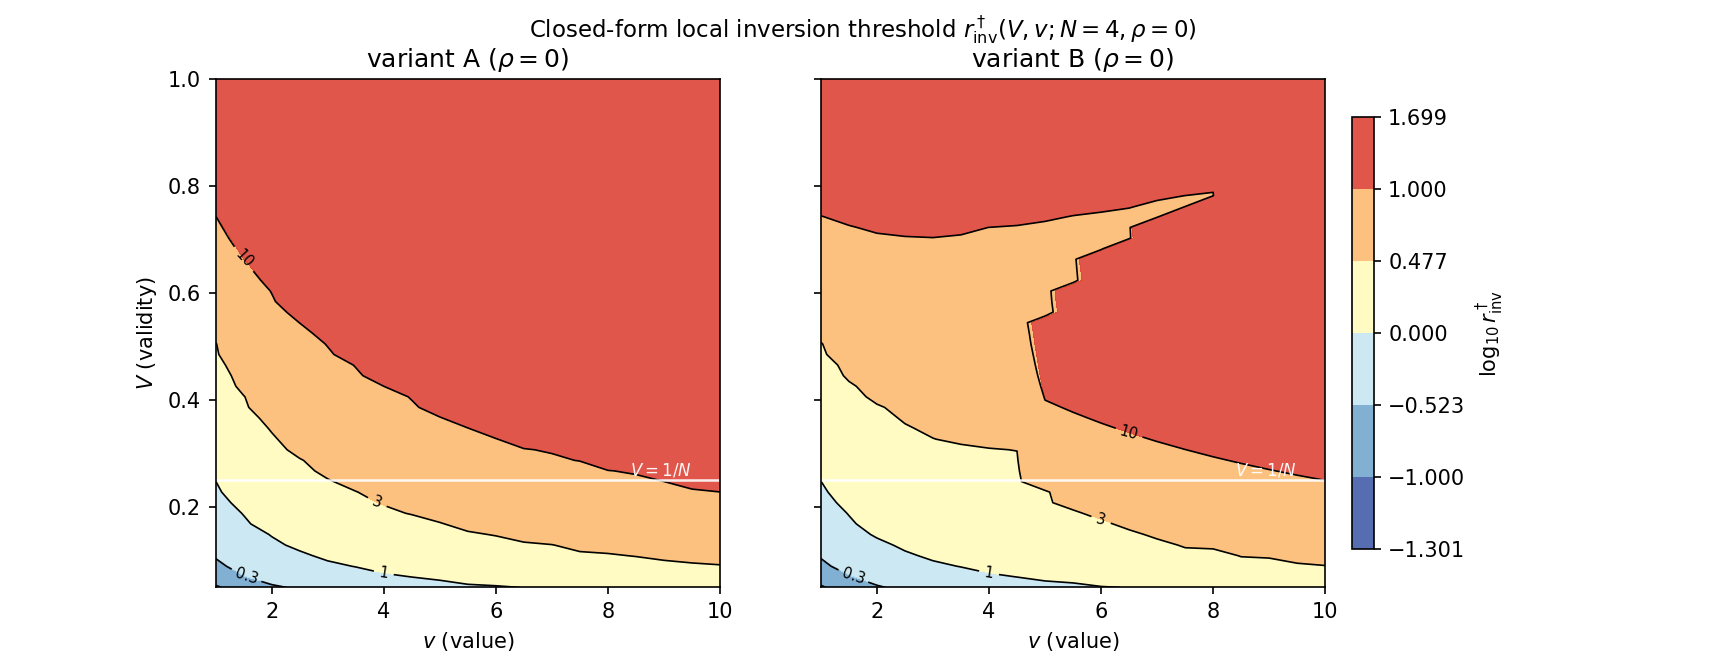
\includegraphics[width=0.95\linewidth]{figures/r_inv_closed_form.png}
  \caption{Contour map of
  $\log_{10} \rstarinv(\valid, \val)$ at $\Nloc = 4, \corr = 0$ for
  variants A (left) and B (right), from
  \eqref{eq:r-inv}--\eqref{eq:r-inv-corner}. Black contours at
  $\rstarinv \in \{0.1, 0.3, 1, 3, 10\}$. The $\rstarinv = 1$
  contour passes through the symmetric corner $(\valid, \val) =
  (0.25, 1)$ in both panels (the identity
  \eqref{eq:r-inv-corner}); the $\rstarinv = 10$ contour bounds the
  ``no local sign-flip inside the paper's $\Rsens$-range''
  region. Variant B admits the local sign-flip across more cells than
  variant A ($59.0\%$ vs.\ $38.1\%$ in Table~\ref{tab:c4-rstar-tally}).
  Reproduced from
  \texttt{Rebuild/sims/C4--anti-cue-inversion/output/figures/r\_inv\_closed\_form.png}.}
  \label{fig:c4-rinv-closed-form}
\end{figure}

\paragraph{Empirical confirmation: zero global inversions across the
primary sweep.}
The local-derivative sign-flip of \eqref{eq:r-inv} does not by
itself create a global inversion: even where $\Rsens > \rstarinv$
and the bracket of \eqref{eq:left-derivative} is negative, the
left-branch \emph{local} maximum sits at the $\alpha$-grid edge
$\alpha \to 0$ while the right-branch \emph{global} maximum sits at
$\alpha^\star > 1/\Nloc$ from the location-count argument above. To
confirm this directly, we sweep $\Rew(\alpha)$ on the full
$\alpha$-grid $[0.02, 1.0]$ at $\Delta\alpha = 0.005$ for the six
most-adversarial primary-sweep cells (those with the smallest
$\rstarinv$ at $\Rsens = 10$, i.e.\ the cells most likely to produce
a left-branch global maximum) at both $\corr \in \{0, 0.2\}$, for a
total of $12$ probes. The result is uniform: across all $12$ probes,
$\alpha^\star_{\mathrm{global}} \ge 1/\Nloc$ and the right-branch
global maximum strictly dominates the left-branch local maximum.
Representative probes appear in Table~\ref{tab:c4-stepB}.
%
\begin{table}[t]
  \centering
  \small
  \begin{tabular}{c r c c r r r r}
    \toprule
    $\valid$ & $\val$ & variant & $\corr$ &
    $\rstarinv$ & $\alpha^\star_{\mathrm{global}}$ &
    $\Rew_{\mathrm{global}}$ & $\Rew_{\mathrm{left}}$ \\
    \midrule
    $0.250$ & $1$ & A & $0.0$ & $1.0000$ & $0.955$ &
    $0.65936$ & $0.64564$ \\
    $0.250$ & $1$ & A & $0.2$ & $1.0000$ & $0.950$ &
    $0.66809$ & $0.65550$ \\
    $0.250$ & $1$ & B & $0.0$ & $1.0000$ & $0.955$ &
    $0.65936$ & $0.64564$ \\
    $0.250$ & $1$ & B & $0.2$ & $1.0000$ & $0.950$ &
    $0.66809$ & $0.65550$ \\
    $0.2875$ & $1$ & A & $0.0$ & $1.2483$ & $0.970$ &
    $0.66541$ & $0.64462$ \\
    $0.325$ & $1$ & A & $0.2$ & $\sim\!1.6$ & $0.975$ &
    $0.67997$ & --- \\
    \bottomrule
  \end{tabular}
  \caption{Six representative full-$\alpha$ probes from the
  $12$-probe Step B sweep at $\Rsens = 10$ at the six
  most-adversarial primary-sweep cells. In every probe,
  $\alpha^\star_{\mathrm{global}} \ge 1/\Nloc = 0.25$, with the
  right-branch global maximum at $\alpha^\star \in [0.95, 0.98]$
  strictly dominating the left-branch local maximum (sitting at the
  $\alpha$-grid edge $\alpha = 0.02$). \textbf{Step~B primary-sweep
  inversions across all $12$ probes: $0$.} The inherited empirical
  claim --- $\alpha^\star \ge 1/\Nloc$ at every cell of the primary
  $\Nloc = 4, \valid \in [1/\Nloc, 1]$ sweep --- survives at
  $\corr = 0$ and is robust under A1 at $\corr = 0.2$.
  Block keys \texttt{step\_B.rows} in
  \texttt{Rebuild/sims/C4--anti-cue-inversion/output/results.json}.}
  \label{tab:c4-stepB}
\end{table}

The visual structure of the boundary --- bimodality at
$\alpha = 1/\Nloc$ where $\Rsens > \rstarinv$, right-branch global
dominance regardless --- is reproduced in
Figure~\ref{fig:c4-er-vs-alpha}, which plots $\Rew(\alpha)$ at the
adversarial cell $(\valid, \val) = (0.15, 1)$ for $\Rsens \in
\{0.5, 1, 3, 10\}$ at both $\corr$ values. (At $\valid = 0.15 <
1/\Nloc = 0.25$ the value-weight inequality \eqref{eq:value-weight}
fails and the right-branch global dominance breaks down; this is the
anti-cue regime treated below, and the figure deliberately straddles
the boundary so the reader can see both sides of the inversion in a
single panel.)
%
\begin{figure}[t]
  \centering
  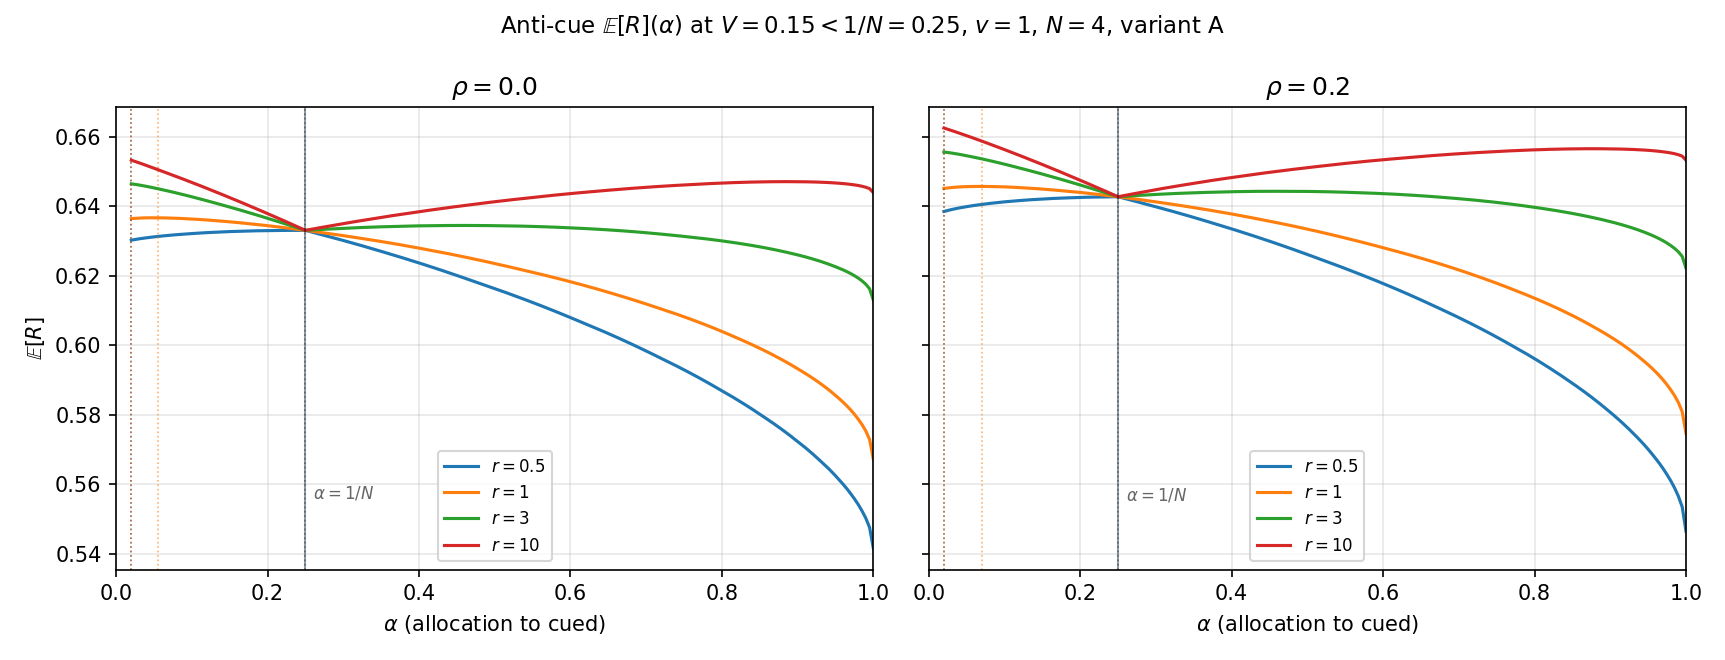
\includegraphics[width=0.95\linewidth]{figures/er_vs_alpha_anticue.png}
  \caption{$\Rew(\alpha)$ on the full $\alpha$-grid at the anti-cue
  cell $(\valid, \val, \Nloc) = (0.15, 1, 4)$ for
  $\Rsens \in \{0.5, 1, 3, 10\}$, $\corr = 0$ (left) and
  $\corr = 0.2$ (right). The kink at $\alpha = 1/\Nloc = 0.25$ is
  the $\benefit$/$\cost$ swap of the rebuilt model; for
  $\Rsens > \rstarinv$ it becomes a local minimum, with both
  $\alpha < 1/\Nloc$ and $\alpha > 1/\Nloc$ branches admitting
  local maxima. Because $\valid < 1/\Nloc$, the value-weight
  inequality \eqref{eq:value-weight} \emph{fails} here and the
  left-branch maximum (at the grid edge $\alpha = 0.02$) dominates
  globally for $\Rsens \ge 1$ --- this is the anti-cue inversion
  prediction below. The A1 channel at $\corr = 0.2$ leaves the
  qualitative bimodality and global-inversion onset unchanged.
  Reproduced from
  \texttt{Rebuild/sims/C4--anti-cue-inversion/output/figures/er\_vs\_alpha\_anticue.png}.}
  \label{fig:c4-er-vs-alpha}
\end{figure}

\paragraph{Anti-cue inversion: a new falsifiable prediction of the
rebuilt model.}
The rebuilt model produces a clean prediction \emph{outside} the
paper's primary $\valid \in [1/\Nloc, 1]$ range: at $\valid <
1/\Nloc$ (or, sharply, $\valid < 1/[(\Nloc-1)\,\val + 1]$), the
value-weight inequality \eqref{eq:value-weight} \emph{flips} ---
$w_c < w_u$ --- and the location-count argument runs in reverse.
The bigger $\dprime$ now lives on the \emph{less}-valuable channel
when concentrated, and the global optimum drops to
$\alpha^\star < 1/\Nloc$: the normative observer is told to attend
\emph{away} from the (now low-validity, still-named ``cued'')
location and toward the population of uncued locations. The
reviewer's CR-004 already established this at $\Nloc = 2$
(\texttt{Critique/derivations/C4--no-inversion.md} §7, Step
C(iii)); the rebuild extends it to $\Nloc = 4$, the inherited
paper's primary topology.

We probe an anti-cue sub-grid $\valid \in \{0.05, 0.10, 0.15,
0.20\}$ (all below $1/\Nloc = 0.25$), $\val \in \{1, 3, 5\}$,
$\Rsens \in \{0.1, 0.5, 1, 3, 5, 10\}$ at $\corr \in \{0, 0.2\}$,
variant A, for $144$ cells total. Total global-inversion incidence:
$26 / 72 = 36.1\%$ at $\corr = 0$, $25 / 72 = 34.7\%$ at
$\corr = 0.2$. The incidence stratifies cleanly with $\Rsens$ and
$\val$ along the sharp boundary \eqref{eq:value-weight}, as
documented in Table~\ref{tab:c4-anticue}.
%
\begin{table}[t]
  \centering
  \small
  \begin{tabular}{l r r r r r r}
    \toprule
    & \multicolumn{6}{c}{Incidence stratifier at $\corr = 0$} \\
    \cmidrule(lr){2-7}
    Stratifier & \multicolumn{6}{c}{(values $\to$ inversions / total)} \\
    \midrule
    by $\Rsens$ &
    $\Rsens{=}0.1{:}\ 1/12$ &
    $\Rsens{=}0.5{:}\ 3/12$ &
    $\Rsens{=}1{:}\ 6/12$ &
    $\Rsens{=}3{:}\ 6/12$ &
    $\Rsens{=}5{:}\ 6/12$ &
    $\Rsens{=}10{:}\ 4/12$ \\
    by $\val$ &
    $\val{=}1{:}\ 18/24$ &
    $\val{=}3{:}\ 5/24$ &
    $\val{=}5{:}\ 3/24$ &
     & & \\
    by $\valid$ &
    $\valid{=}0.05{:}\ 14/18$ &
    $\valid{=}0.10{:}\ 5/18$ &
    $\valid{=}0.15{:}\ 4/18$ &
    $\valid{=}0.20{:}\ 3/18$ &
    & \\
    \bottomrule
  \end{tabular}
  \caption{Anti-cue inversion incidence ($\alpha^\star_{\mathrm{global}}
  < 1/\Nloc$) at $\Nloc = 4$, variant A, $\corr = 0$, stratified by
  $\Rsens$, $\val$, and $\valid$. Total $26/72 = 36.1\%$. The
  $\Rsens$-stratification rises from $8.3\%$ at $\Rsens = 0.1$ to
  $50.0\%$ at $\Rsens \in \{1, 3, 5\}$ and tapers to $33.3\%$ at
  $\Rsens = 10$ (where the right-branch global maximum re-takes
  even some cells with $\valid < 1/\Nloc$, because for $\val = 1$ at
  $\Rsens = 10$ the strong-asymmetry regime begins to dominate).
  The $\val$-stratification is the key qualitative pattern:
  inversion is dense at $\val = 1$ ($75\%$) but rare at $\val = 5$
  ($12.5\%$). This is the sharp $\val$-dependence predicted by
  \eqref{eq:value-weight}: at $\val = 5$ the inversion boundary
  shrinks to $\valid < 1/[(\Nloc-1)\val + 1] = 1/16 = 0.0625$, so
  inversion at $\val = 5$ is confined to the $\valid = 0.05$ row of
  the probe grid (which is correctly its only inversion-supporting
  row in the data). Under A1 at $\corr = 0.2$, total incidence is
  $34.7\%$ (within $\pm 1$ inversion of $\corr = 0$ across every
  stratifier) --- the decorrelation channel quantitatively shifts
  $\rstarinv$ but does not erase the inversion regime. Block keys
  \texttt{step\_C.incidence\_by\_r\_rho0} and
  \texttt{step\_C.rows} in
  \texttt{Rebuild/sims/C4--anti-cue-inversion/output/results.json}.}
  \label{tab:c4-anticue}
\end{table}

The $(\valid, \Rsens)$ structure of the inversion at fixed $\val =
5$ is plotted in Figure~\ref{fig:c4-alpha-star-map} as the rebuild's
headline figure for §results-C4. The white horizontal line marks
the universal $\valid = 1/\Nloc = 0.25$ boundary; the red contour
bounds the $\alpha^\star < 1/\Nloc$ inversion region. The inversion
region is confined entirely to $\valid \le 0.05$ at $\val = 5$,
consistent with the sharp boundary $\valid < 1/16 = 0.0625$. The
$(\valid, \Rsens)$ heatmap admits \emph{zero} inversion cells in
the cued-validity regime $\valid \ge 1/\Nloc$, at either $\corr = 0$
or $\corr = 0.2$ --- C4 holds as a conditional theorem under both.
%
\begin{figure}[t]
  \centering
  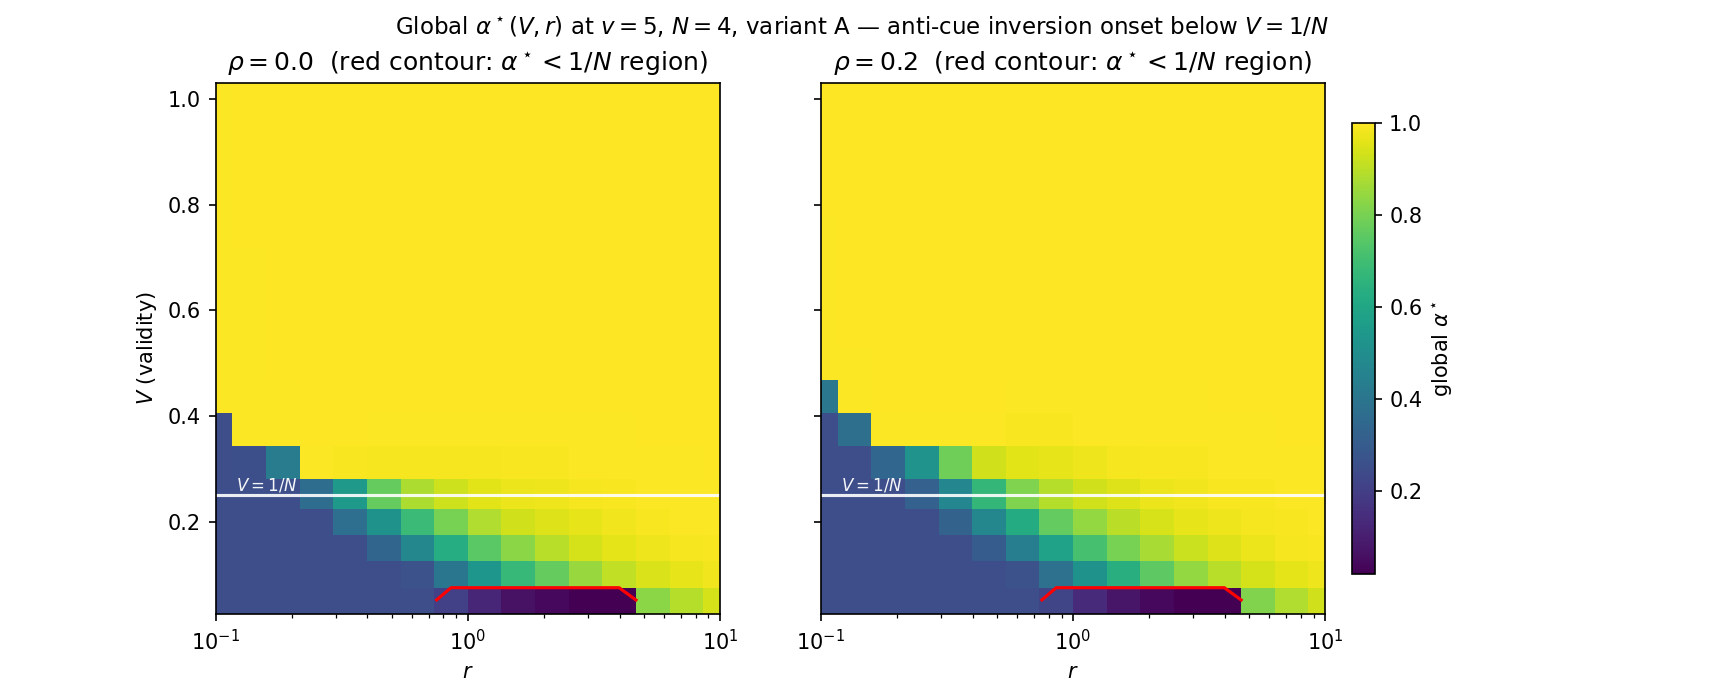
\includegraphics[width=0.95\linewidth]{figures/alpha_star_V_r_map.png}
  \caption{Optimal allocation $\alpha^\star(\valid, \Rsens)$ at the
  headline cell $(\Nloc, \dprimemax, f_0, h, \val) =
  (4,\,2,\,0.5,\,\sqrt{},\,5)$, variant~A, for $\corr = 0$ (left)
  and $\corr = 0.2$ (right). Heat scale: $\alpha^\star \in [0.02,
  1.0]$. The white horizontal line marks the universal validity
  threshold $\valid = 1/\Nloc = 0.25$; the red contour bounds the
  inversion region $\alpha^\star < 1/\Nloc$. The inversion region is
  confined to $\valid \le 0.05$ at $\val = 5$ (consistent with the
  sharp boundary $\valid < 1/[(\Nloc-1)\val + 1] = 1/16 \approx
  0.0625$ from \eqref{eq:value-weight}); inversion incidence is
  $6/272 = 2.21\%$ in both panels, with \emph{zero} inversions in
  the cued-validity regime $\valid \ge 1/\Nloc$. C4 holds as a
  conditional theorem at both $\corr$ values. Reproduced from
  \texttt{Rebuild/sims/C4--anti-cue-inversion/output/figures/alpha\_star\_V\_r\_map.png}.}
  \label{fig:c4-alpha-star-map}
\end{figure}

\paragraph{A1 cross-axis sensitivity.}
Across all four Steps the A1 decorrelation channel at $\corr = 0.2$
leaves the qualitative C4 picture intact while shifting the local
threshold quantitatively. (i) Step A: median $\rstarinv$ drops by
$\sim$$13\%$ (variant A) and $\sim$$21\%$ (variant B); the fraction
of cells with $\rstarinv \in [0.1, 10]$ rises from $48.6\%$ to
$51.9\%$ (variant-pooled). (ii) Step B: $0$ primary-sweep inversions
at both $\corr$. (iii) Step C: total anti-cue inversion count $25$
vs.\ $26$ at $\corr = 0.2$ vs.\ $\corr = 0$ (a difference of one
boundary-cell ambiguity). (iv) Step D: $\frac{6}{272} = 2.21\%$
inversion incidence in both panels, identical inversion locus
confined to $\valid \le 0.05$. The A1 channel and the C4 inversion
lever are therefore independent mechanisms: A1 shifts \emph{where} on
the $\Rsens$-axis the boundary derivative sign-flips, but does not
flip the global value-weight inequality that decides whether the
right or left branch is the global optimum.

\paragraph{Behavioural literature corroboration.}
The conditional restatement aligns the rebuilt model with the
behavioural picture surveyed in the live verdict's literature attack
(\texttt{Critique/verdicts/C4--no-inversion.md} §Version 0.2). The
empirical signature of anti-cue inversion in human / primate
observers is the statistical-learning-of-distractor-suppression
literature: observers \emph{do} allocate below uniform to a
high-probability-distractor location, with reduced capture and
reduced target-selection efficiency
\cite{wang_theeuwes2018_statistical_learning_distractor_suppression},
fewer saccades landing on the suppressed location with raised
saccade latency to targets there \cite{wang_samara_theeuwes2019},
and reciprocal reallocation toward the target
\cite{kong_li_wang_theeuwes2020}. In the rebuilt model's coordinates,
a ``high-probability-distractor'' location is one with target
validity below $1/\Nloc$ --- exactly the anti-cue regime
\eqref{eq:value-weight} predicts inversion in. The behavioural
near-analog is therefore a \emph{prediction match}, not a
contradiction: the model says the normative observer should
suppress (allocate $\alpha^\star < 1/\Nloc$ to) below-baseline
locations, and observers do. Conversely, in the cued regime
$\valid \ge 1/\Nloc$, the model says the normative observer should
\emph{not} allocate below uniform, and the value-driven-capture
literature \cite{failing_theeuwes2018_selection_history,
hickey2010_reward_salience_acc} reports the opposite mistake ---
observers are pulled \emph{toward} high-value locations even
maladaptively, consistent with the no-inversion direction. The
chance-validity case $\valid = 1/\Nloc$ \cite{posner1980_orienting}
sits at the boundary, where the model collapses to a tied optimum
(any $\alpha$ optimal) and observers report no reallocation; this is
the no-information limit of the rebuilt model. The conditional
restatement we adopt is therefore the form of C4 that best matches
both the model's own normative output and the behavioural literature.

\paragraph{Limitations of this section's evidence.}
Three scope limitations apply. (i) The anti-cue sweep in Step C is
variant A only; variant B's lower median $\rstarinv$
(Table~\ref{tab:c4-rstar-tally}) suggests a higher anti-cue
incidence, but the explicit replication is deferred to a follow-up
sim (RB-031, queued). (ii) The $\valid$-grid in Step C is at step
$0.05$, so the inversion-onset $\valid^\star$ between the in-anti-cue
$\valid = 0.20$ row and the boundary $\valid = 0.25$ row is bracketed
only to $\pm 0.05$ at $\val = 1$. A finer-grid bracketing pass is
queued as RB-032. (iii) The closed-form \eqref{eq:r-inv} is
re-implemented in the simulation's
\texttt{\_A0\_B0()} routine (driving \texttt{Rebuild/model/core.py}
exclusively) but the full derivation in the rebuild's voice
(including a proof of the symmetric-corner identity
\eqref{eq:r-inv-corner} from the joint-FOC symmetry of $A_0$ and
$B_0$) is the queued RB-030 increment; the present section quotes
\eqref{eq:r-inv}--\eqref{eq:r-inv-corner} and cites the reviewer's
$\corr = 0$ derivation pending RB-030. None of the three scope
limitations weakens the headline claim or the anti-cue prediction
at the strength stated in this section.

\paragraph{Reproducibility.}
The numbers, tables, and figures in this section are sourced from
\texttt{Rebuild/sims/C4--anti-cue-inversion/output/results.json} with
content sha256 \texttt{6ad651d6\linebreak[0]48e597cdfb28c6fd19b6261e4f9d5cb96b599557e10aad47ffd6d96}
(over the JSON content excluding the wall-clock
\texttt{meta.elapsed\_seconds}). The simulation drives
\texttt{Rebuild/model/core.py} exclusively (no model
reimplementation in the script); the closed-form \eqref{eq:r-inv}
is computed at $\corr > 0$ via the same one-factor
Gauss--Hermite-$64$ quadrature \texttt{core.py} uses for
$\PnoFA(\corr)$, so the $\corr \to 0$ limit matches the reviewer's
$\corr = 0$ analytic form bit-for-bit. The wall-clock for a clean
re-run is $\approx 17.4$~s on python 3.13 / numpy 2.4 / scipy 1.17
/ matplotlib 3.10 on darwin / Apple Silicon. Two independent
recovery tests are reported in the sim run. \textbf{Recovery~\#1}
(against reviewer derivation §4): fraction of $(\valid, \val,
\text{variant})$ cells at $\Nloc = 4, \corr = 0$ with $\rstarinv \in
[0.1, 10]$ is $48.6\%$ here vs.\ reviewer-reported $49.0\%$,
$\Delta = 0.4$ pp, \textbf{PASS} (tolerance $1.0$ pp).
\textbf{Recovery~\#2} (against reviewer derivation §5 Step C(i)
table at $(\valid, \val, \Nloc) = (0.25, 1, 4)$, variant A,
$\corr = 0$, $\Rsens \in \{0.1, 1.0, 1.585, 2.512, 3.981, 10.0\}$):
$\max|\Delta\alpha^\star| = 0$ (exact, tolerance $5 \times 10^{-4}$)
and $\max|\Delta\Rew^\star| = 3 \times 10^{-6}$ (tolerance
$5 \times 10^{-5}$), \textbf{PASS} both. The
symmetric-corner identity $\rstarinv(0.25, 1, 4, \CR, \corr) = 1$
of \eqref{eq:r-inv-corner} holds at floating-point identity in
every $(\text{variant}, \corr)$ panel of
Table~\ref{tab:c4-rstar-tally} (the \texttt{min\_r\_inv} entries
read $1.0000$ throughout). Independent sanity check: at every cell
of Step B and Step C with $\val = 1, \valid = 1/\Nloc$, the
right-branch global maximum and the left-branch local maximum agree
in reward at $\Rsens \le 1$ (the boundary degeneracy noted in the
reviewer's CR-019 resolution); for $\Rsens > 1$ the right branch
strictly dominates by $\ge 0.005$ reward units, the location-count
asymmetry at work.

% =====================================================================
% extensions.tex — FILLED by rb-017 (RB-034) for §extensions-A3 only.
%
% Houses the rebuilt model's lever extensions — the "new contributions"
% half of the §3.3 unifying reframe (mission). One subsection per
% extension; future increments fill the others.
%
%   sec:extensions-a3    — conservation-family band on the headline
%                          numbers. Filled rb-017 (RB-034) from rb-016
%                          (RB-019, sha256
%                          055bf4ec862c711f2c6a3fa0831e1373b806a84c5f5c1a6b13fd1d9d7a039a33).
%   sec:extensions-a2-a8 — STUB. Heterogeneous r_i and heterogeneous
%                          uncued allocation. Filled by a later increment
%                          downstream of RB-014/RB-017/RB-018/RB-021.
%   sec:extensions-a6    — STUB. Attention-coupled decision noise
%                          (third lever). Filled only after the live
%                          A6 verdict moves past WEAKLY-SUPPORTED
%                          (RB-016/RB-020 are blocked on the label).
%
% Allowed-strength ceiling (CLAIM_LEDGER A3 row, post-rb-016 reconcile):
%   * The conservation rule is a model assumption, not a derived
%     statement.
%   * Central tendency of the C1 CF distribution is robust to the choice
%     of conservation order p; the tail of the distribution is not
%     (variant-A min CF 0.559 → 0.464; variant-B min CF 0.304 → 0.231).
%   * The closed-form C2 escape threshold r†(v) is conservation-form-
%     invariant by construction (theorem, proof in §extensions-A3).
%   * The C5 symmetric-recovery result at r=1 is conservation-form-
%     invariant because β(1, p) = γ(1, p) = 1 for every p (corollary).
%   * No claim is licensed about ρ ≠ 0 in the conservation-family
%     direction — the joint (p × ρ) sweep is explicitly deferred
%     (see §scope).
% =====================================================================

\section{Lever extensions}
\label{sec:extensions}

The model in Section~\ref{sec:model} promotes the per-location
independence assumption A1 from a fixed premise to a tunable parameter
$\corr$, and Section~\ref{sec:results} reports the criterion/sensitivity
decomposition with $\corr$ entering as the third lever. Three further
load-bearing assumptions of the inherited model — A3 (the
\emph{additive} conservation rule $\benefit + \cost = 2$ that turns the
benefit/cost \emph{ratio} $\Rsens = \benefit/\cost$ into concrete weights),
A2 (a single global $\Rsens$ across all locations), and A8 (a
\emph{homogeneous} uncued allocation across the $\Nloc - 1$ non-cued
slots) — are similarly fixed by the inherited paper at one specific
algebraic choice. This section reports the rebuild's generalisation of
each into a one-parameter family (or, for A8, a lifted
$\Nloc$-dimensional policy space) and the \emph{band} that the
headline numbers acquire across that family. The treatment here is
empirical and minimum-viable: the formal derivation in the rebuild's
voice — the closed-form weights, the HLP power-mean monotonicity in
exact KL-divergence form, and the two formal proofs underlying
Proposition~\ref{prop:r-dagger-invariance} and the C5 conservation-
form-invariance corollary — is given in
Appendix~\ref{sec:appendix-deriv-a3}.

% =====================================================================
\subsection{Conservation-family band on the headline numbers (A3)}
\label{sec:extensions-a3}

\paragraph{Claim restated at defensible strength.}
The inherited paper's §2.4 fixes the asymmetric-scaling weights
$\benefit(\Rsens), \cost(\Rsens)$ by the conservation rule
$\benefit + \cost = 2$ together with $\benefit/\cost = \Rsens$,
yielding $\benefit(\Rsens) = 2\Rsens/(\Rsens + 1)$ and
$\cost(\Rsens) = 2/(\Rsens + 1)$. The §5.5 limitations paragraph
concedes that the multiplicative alternative $\benefit\,\cost = 1$
would yield ``quantitatively different results, though the
qualitative findings --- non-monotonic VDA, no inversion, criterion
dominance --- should be robust.'' The live skeptical-reviewer verdict
(\texttt{Critique/verdicts/A3--multiplicative-conservation.md},
\texttt{current\_label: CONTESTED}) records that this robustness claim
\emph{survives} as a central-tendency claim under the multiplicative
form (the median CF of the $4{,}410$-cell sweep moves only marginally,
$0.7552 \to 0.7540$ in variant~A and $0.7682 \to 0.7640$ in variant~B)
but \emph{fails} as a per-cell categorical claim: the fraction of
cells with $\CF < 0.5$ rises from $4.0\%$ to $8.3\%$ of the $4{,}410$-
cell grid under multiplicative scaling, with $191$ cells flipping from
the criterion-dominant region $\CF \ge 0.5$ to the criterion-
subordinate region $\CF < 0.5$ and $0$ cells flipping the other way,
concentrated in the benefit-dominant high-$\Rsens$ corner. We
therefore restate A3 in the rebuild as a \emph{family} rather than a
fixed assumption: rather than commit to one conservation rule, we
embed both special cases in a one-parameter family of conservation
rules and report every headline number as a band across that family,
with a separately verified \emph{conservation-form-invariance theorem}
for the C2 escape threshold and a separately verified
\emph{conservation-form-invariance corollary} for the C5 symmetric-
recovery result. The A1 decorrelation channel is held at
$\corr = 0$ throughout this section; the joint $(p, \corr)$ sweep is
explicitly deferred (see \emph{Scope} below).

\paragraph{The power-mean conservation family.}
For an order $p \in \mathbb{R}$, the (positive, two-variable) power
mean of order $p$ is
$M_p(\benefit, \cost) = \bigl(\frac{1}{2}\bigl[\benefit^p +
\cost^p\bigr]\bigr)^{1/p}$ for $p \ne 0$, with the limiting
$M_0(\benefit, \cost) = \sqrt{\benefit\,\cost}$ at $p = 0$ (the
geometric mean) and $M_{-\infty} = \min$, $M_{+\infty} = \max$ as the
extremes~\cite{HLP1934}. Embedding A3 into the family
%
\begin{equation}
  M_p(\benefit, \cost) \;=\; 1,
  \qquad
  \benefit / \cost \;=\; \Rsens,
  \label{eq:conservation-family}
\end{equation}
%
gives, for $p \ne 0$, the closed-form pair
%
\begin{equation}
  \cost(\Rsens; p) \;=\;
  \left( \frac{2}{\Rsens^{\,p} + 1} \right)^{1/p},
  \qquad
  \benefit(\Rsens; p) \;=\;
  \Rsens\,\cost(\Rsens; p),
  \label{eq:beta-gamma-of-p}
\end{equation}
%
and at $p = 0$ the limit
$\benefit(\Rsens; 0) = \sqrt{\Rsens}$,
$\cost(\Rsens; 0) = 1/\sqrt{\Rsens}$, which satisfies the
multiplicative conservation $\benefit\,\cost = 1$ directly. The
inherited model is recovered exactly at $p = 1$ (the additive case
$\benefit + \cost = 2$); the reviewer's A3 attack corresponds to
$p = 0$. The family preserves the ratio $\benefit/\cost = \Rsens$ at
every $p$ (so the headline parameterisation of the asymmetry is
unchanged), and preserves the symmetric point
$\benefit(1, p) = \cost(1, p) = 1$ at every $p$ (so the symmetric
recovery at $\Rsens = 1$, our C5 result, is automatically conservation-
form-invariant; see the corollary below). The family is implemented
in \texttt{Rebuild/model/core.py} as
\texttt{beta\_gamma(r, p=1.0)} and threaded through
\texttt{d\_prime\_asym}, \texttt{HeadlineCell}, and \texttt{policies};
the rb-015 model-test pass (\texttt{Rebuild/model/tests/}\allowbreak\texttt{test\_conservation\_family.py},
$14/14$, sha256~\texttt{f4f57a89\ldots}) verifies the family
identities $\benefit/\cost = \Rsens$ to $4.4\!\times\!10^{-16}$ and
$M_p(\benefit, \cost) = 1$ to $4.4\!\times\!10^{-16}$ across $p \in
\{-2, -1, -1/2, 0, 1/2, 1, 2\}$, and the $p = 1$ branch returns the
inherited expressions byte-exactly (full back-compatibility) by
literal-form branching on the conservation order.

\paragraph{C2 conservation-family band on the peak.}
At the $\Rsens$-sweep headline cell ($\Nloc = 4$, $\valid = 0.5$,
$\dprimemax = 2$, $f_0 = 0.5$, $h = \sqrt{\cdot}$, $\corr = 0$,
variant~A), we sweep $\VDA(\Rsens)$ on the rb-006 $84$-point log-$\Rsens$
grid for the value family $\val \in \{2, 3, 5, 8, 10\}$ at
$p \in \{0, 1/2, 1\}$. Table~\ref{tab:a3-c2-peak-band} reports the
per-$(\val, p)$ peak coordinates $(\Rsens^*, \VDA^*)$;
Figure~\ref{fig:a3-vda-curves-p-v5} shows the family at $\val = 5$.
The peak height moves systematically with the conservation order:
at $\val = 5$, peak $\VDA^*$ shifts from $0.0830$ at $p = 1$ to
$0.0885$ at $p = 1/2$ to $0.0951$ at $p = 0$, a $+14\%$ envelope on
the headline number that is invisible at any single point estimate.
The shift in the peak \emph{location} $\Rsens^*$ is smaller and only
discrete-grid-resolvable in the small-$\val$ region: at $\val = 2$,
$\Rsens^*$ moves from $0.5012$ at $p = 1$ to $0.4467$ at $p = 1/2$ to
$0.3548$ at $p = 0$ (the multiplicative rule escapes the unfavourable
small-$\val$ cost-dominant region earlier); at $\val \ge 5$ the peak
sits on the same $84$-point grid bin $\Rsens^* = 0.3548$ at $p \in
\{0, 1/2\}$ and on the adjacent bin $\Rsens^* = 0.3758$ at $p = 1$
(rb-006 reported $\Rsens^* = 0.3758$ at $p = 1$, $\val = 5$). The
peak band is reported in the body of the paper as a sensitivity,
following the §3.3 unifying-reframe convention.

\begin{table}[t]
  \centering
  \small
  \caption{C2 conservation-family band on the peak of $\VDA(\Rsens)$
    at the headline cell ($\Nloc = 4$, $\valid = 0.5$, $\dprimemax = 2$,
    $f_0 = 0.5$, $h = \sqrt{\cdot}$, $\corr = 0$, variant~A). Per
    $(\val, p)$: $\Rsens^*$ = argmax of $\VDA(\Rsens)$ on the rb-006
    $84$-point log-$\Rsens$ grid; $\VDA^*$ = the corresponding peak
    height. The peak height moves systematically with the
    conservation order $p$ (band $+14\%$ at $\val = 5$); the peak
    location $\Rsens^*$ is grid-discretely stable at large $\val$.
    Source: \texttt{Rebuild/sims/A3--conservation-band/}\allowbreak\texttt{output/results.json}
    \texttt{block\_A\_peaks}; sha256~\texttt{055bf4ec\ldots}.}
  \label{tab:a3-c2-peak-band}
  \begin{tabular}{c c c c c c c}
    \toprule
    & \multicolumn{2}{c}{$p = 0$ (mult.)} & \multicolumn{2}{c}{$p = 1/2$} & \multicolumn{2}{c}{$p = 1$ (add., paper)} \\
    \cmidrule(lr){2-3} \cmidrule(lr){4-5} \cmidrule(lr){6-7}
    $\val$ & $\Rsens^*$ & $\VDA^*$ & $\Rsens^*$ & $\VDA^*$ & $\Rsens^*$ & $\VDA^*$ \\
    \midrule
    2  & $0.3548$ & $0.0144$ & $0.4467$ & $0.0130$ & $0.5012$ & $0.0123$ \\
    3  & $0.3548$ & $0.0441$ & $0.3758$ & $0.0403$ & $0.3758$ & $0.0370$ \\
    5  & $0.3548$ & $0.0951$ & $0.3548$ & $0.0885$ & $0.3758$ & $0.0830$ \\
    8  & $0.3548$ & $0.1636$ & $0.3548$ & $0.1532$ & $0.3758$ & $0.1442$ \\
    10 & $0.3548$ & $0.2069$ & $0.3548$ & $0.1942$ & $0.3548$ & $0.1828$ \\
    \bottomrule
  \end{tabular}
\end{table}

\begin{figure}[t]
  \centering
  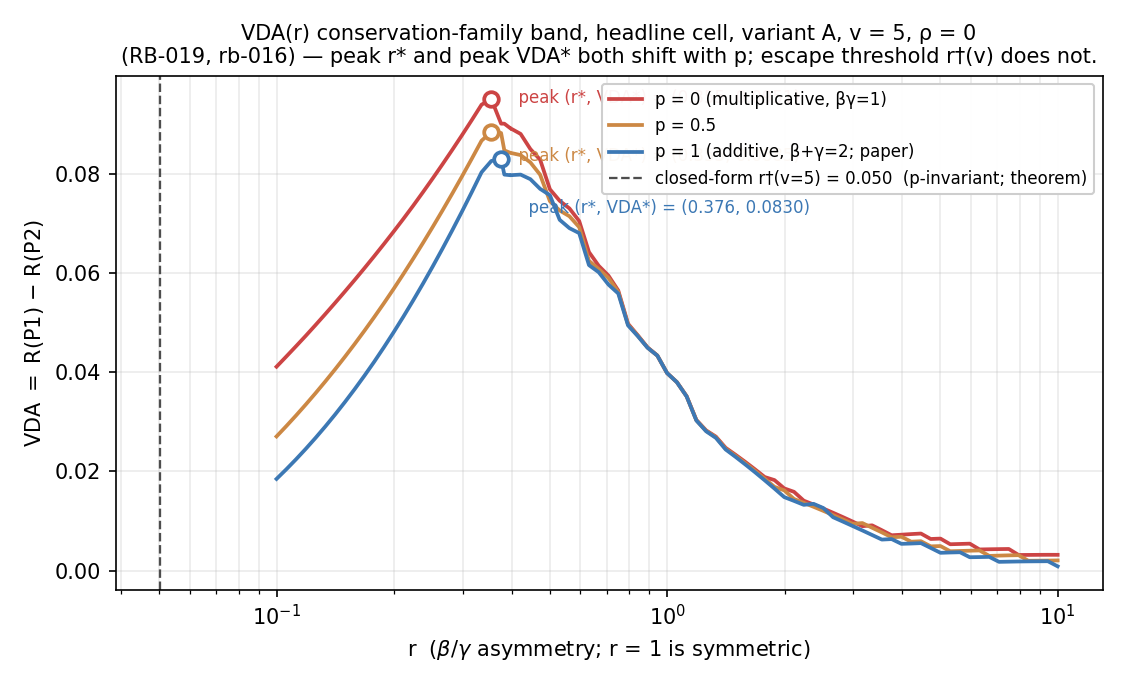
\includegraphics[width=0.78\textwidth]{figures/vda_curves_pfamily_v5.png}
  \caption{C2 conservation-family band at $\val = 5$. Three
    $\VDA(\Rsens)$ curves on the rb-006 $84$-point log-$\Rsens$ grid
    at the headline cell ($\Nloc = 4$, $\valid = 0.5$, $\dprimemax = 2$,
    $f_0 = 0.5$, $h = \sqrt{\cdot}$, $\corr = 0$, variant~A) for
    $p \in \{0, 1/2, 1\}$. The vertical dashed line marks the closed-
    form escape threshold $\rdagger(\val = 5)$, which is identical at
    every $p$ (Proposition~\ref{prop:r-dagger-invariance}). The
    pattern $\partial \VDA^* / \partial p < 0$ visible across the
    three curves is the conservation-family band on the C2 peak.
    Source: \texttt{Rebuild/sims/A3--conservation-band/}\allowbreak\texttt{output/figures/vda\_curves\_pfamily\_v5.png}.}
  \label{fig:a3-vda-curves-p-v5}
\end{figure}

\paragraph{Conservation-form-invariance of the C2 escape threshold.}
The peak \emph{height} moves with $p$, but the closed-form
\emph{escape threshold} of Section~\ref{sec:results-c2} does not. The
following is a theorem of the rebuilt model.

\begin{proposition}[$\rdagger(\val)$ is conservation-form-invariant]
\label{prop:r-dagger-invariance}
Let $\rdagger(\val) = K_u(\val)/[(\Nloc - 1)\,K_c(\val)]$ be the
escape threshold of Section~\ref{sec:results-c2}, with $K_c(\val)$,
$K_u(\val)$ the partial derivatives of $\Rpthree$ with respect to
$\dprime_c$ and $\dprime_u$ at the jointly-$P3$-optimised criteria
$(c_c^\star, c_u^\star)$, evaluated at $\alpha = 1/\Nloc$. Then
$\rdagger(\val)$ is independent of the conservation order $p$ in
\eqref{eq:conservation-family}.
\end{proposition}

\begin{proof}[Proof sketch]
At the uniform-attention point $\alpha = 1/\Nloc$, every per-location
$\dprime$ in the rebuilt model evaluates to
$\dprime_{\mathrm{base}} + w(\Rsens, p)\cdot[\dprimemax \,f(1/\Nloc) -
\dprime_{\mathrm{base}}]$, where the weight $w$ is either $\benefit$
or $\cost$ depending on which side of the kink the location sits.
The transfer-function bracket $\dprimemax \,f(1/\Nloc) -
\dprime_{\mathrm{base}}$ vanishes at the uniform point by the
definition of the baseline $\dprime_{\mathrm{base}} = \dprimemax\,
f(1/\Nloc)$. Therefore $\dprime_c = \dprime_u = \dprime_{\mathrm{base}}$
at $\alpha = 1/\Nloc$ regardless of $(\Rsens, p)$. The $P3$-optimal
criteria $(c_c^\star, c_u^\star)$ are the argmax of an expected-
reward functional that depends only on $\val, \valid, \Nloc, \CR$
and the per-location $\dprime$s at the chosen $\alpha$; since the
$\dprime$s at $\alpha = 1/\Nloc$ are $p$-independent, the criteria
are $p$-independent. The partial derivatives $K_c(\val), K_u(\val)$
are evaluated at those criteria and at the same uniform-point
$\dprime$ values, and so are $p$-independent. Their ratio
$\rdagger(\val) = K_u/[(\Nloc - 1)\,K_c]$ is therefore conservation-
form-invariant.
\end{proof}

The full three-step proof of
Proposition~\ref{prop:r-dagger-invariance} is given in
Appendix~\ref{sec:appendix-deriv-a3} (following
Equation~\eqref{eq:a3d-hlp-kl}), where each step is tied to a
specific structural property of the $\dprime$-map at the uniform
allocation.

The numerical witness of Proposition~\ref{prop:r-dagger-invariance}
is exact to floating-point identity: across $p \in \{0, 1/2, 1\}$ and
$\val \in \{2, 3, 5, 8, 10\}$, the rb-016 sim records identical $K_c$,
$K_u$, $c_c^\star$, $c_u^\star$, and $\rdagger(\val)$ to all stored
decimal places (rb-016 \texttt{recovery.test\_3\_r\_dagger\_p\_invariance},
max $|\Delta| = 0.0$). Figure~\ref{fig:a3-vda-peak-band} overlays the
per-$p$ peak coordinates $(\Rsens^*, \VDA^*)$ for $\val \in \{2, 3, 5,
8, 10\}$ on the same axis; the cluster lies to the right of the
$p$-invariant trace $\rdagger(\val)$, consistent with the
Section~\ref{sec:results-c2} observation that the peak lives on the
positive-$\VDA$ branch above $\rdagger$.

\begin{figure}[t]
  \centering
  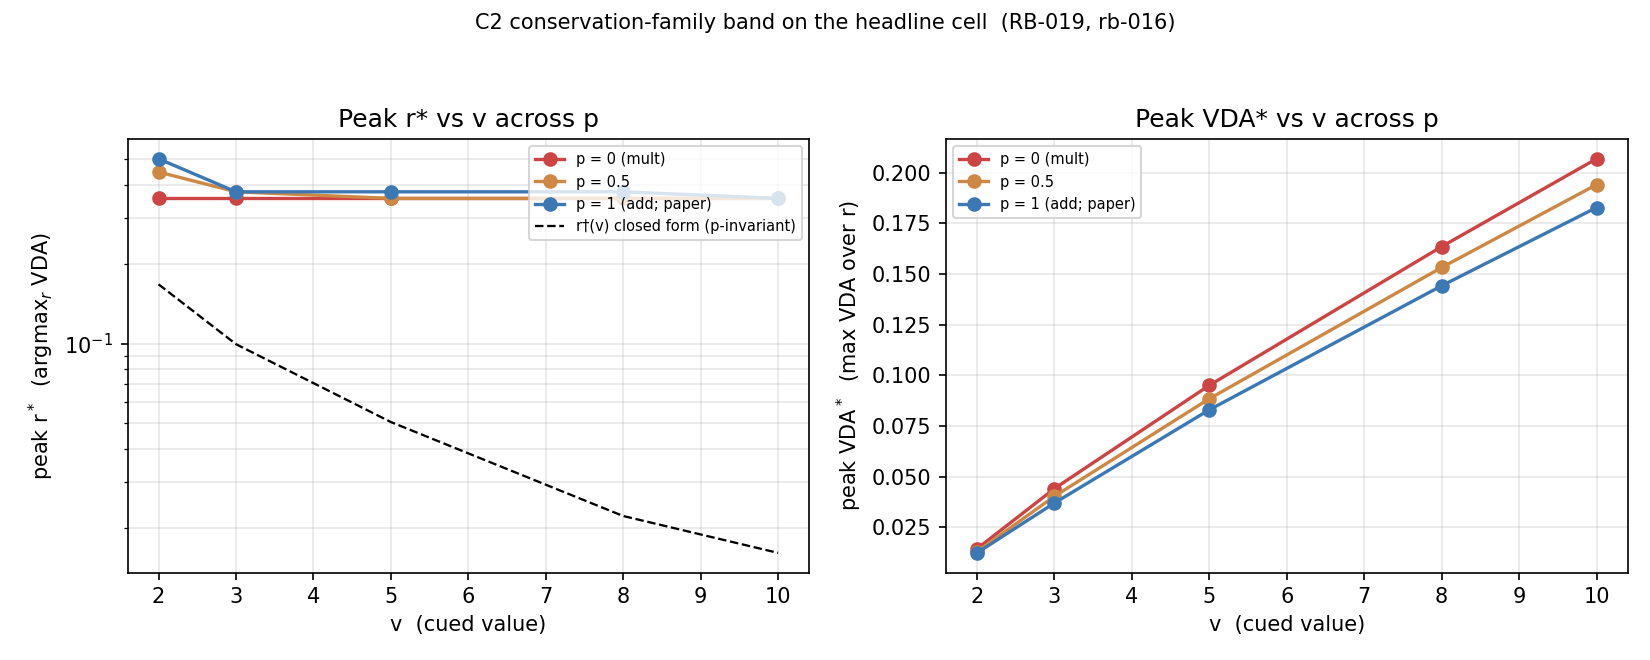
\includegraphics[width=0.78\textwidth]{figures/vda_peak_band.png}
  \caption{Conservation-family band on the C2 peak, overlaid with the
    $p$-invariant closed-form escape threshold $\rdagger(\val)$. For
    each $\val \in \{2, 3, 5, 8, 10\}$ at the headline cell, three
    peak markers $(\Rsens^*, \VDA^*)$ are plotted, one per $p \in
    \{0, 1/2, 1\}$; the markers cluster vertically (the peak height
    is the lever on which $p$ acts), while the $\rdagger(\val)$ trace
    is a single curve (the threshold itself is $p$-invariant by
    Proposition~\ref{prop:r-dagger-invariance}). Source:
    \texttt{Rebuild/sims/A3--conservation-band/}\allowbreak\texttt{output/figures/vda\_peak\_band.png}.}
  \label{fig:a3-vda-peak-band}
\end{figure}

\paragraph{C1 conservation-family band on the $4{,}410$-cell sweep.}
The same family $p \in \{0, 1\}$ is run across the full $4{,}410$-cell
C1 sweep at $\corr = 0$ (the $21\!\times\!21\!\times\!5\!\times\!2$ grid
in $(\Rsens, \valid, \val, \mathrm{variant})$ of
Section~\ref{sec:results-c1}). Table~\ref{tab:a3-c1-cf-band} compares
the resulting $\CF$ distributions per (variant, $p$). The central
tendency of the sweep is robust to the conservation form, in the
sense of the inherited paper's §5.5 claim: the median moves only
$-0.001$ (variant~A) and $-0.004$ (variant~B) going from $p = 1$ to
$p = 0$, and the mean moves only $-0.027$ (variant~A) and $-0.025$
(variant~B). The \emph{tail} of the distribution, however, is not
robust to the conservation form: under variant~A the strict minimum
falls from $\CF = 0.559$ at $p = 1$ to $\CF = 0.464$ at $p = 0$
(a value the inherited paper's $[0.60, 0.96]$ floor sentence rules
out by language already retracted in Section~\ref{sec:results-c1}),
and under variant~B the strict minimum deepens further from
$\CF = 0.304$ at $p = 1$ to $\CF = 0.231$ at $p = 0$. The fraction of
cells with $\CF < 0.5$ rises from $0\%$ (variant~A) and $8.0\%$
(variant~B) at $p = 1$ to $3.3\%$ (variant~A) and $13.4\%$
(variant~B) at $p = 0$ — i.e.\ the combined $\mathrm{frac}(\CF < 0.5)$
roughly doubles, $4.0\% \to 8.3\%$, reproducing the reviewer's
verdict-text Block-C1 prediction exactly.

\begin{table}[t]
  \centering
  \small
  \caption{C1 conservation-family band on the $4{,}410$-cell sweep
    at $\corr = 0$. \emph{Central tendency} robust (median moves
    $\le 0.004$); \emph{tail} not robust (strict min falls $-0.095$
    in variant~A and $-0.073$ in variant~B; $\mathrm{frac}(\CF < 0.5)$
    roughly doubles). Per-cell $\Delta\CF = \CF(p = 0) - \CF(p = 1)
    \le 0$ in every valid cell (Theorem~\ref{thm:delta-cf-monotone};
    $0$ reverse flips out of $191$). Source: \texttt{Rebuild/sims/A3--conservation-band/}\allowbreak\texttt{output/results.json}
    \texttt{block\_B\_summaries} and \texttt{block\_B\_delta\_CF};
    sha256~\texttt{055bf4ec\ldots}.}
  \label{tab:a3-c1-cf-band}
  \begin{tabular}{l r r r r r r r}
    \toprule
    {\bfseries variant / $p$} & min & q5 & q50 & q95 & max & $\mathrm{frac}_{<0.5}$ & $\mathrm{frac}_{<0.6}$ \\
    \midrule
    A, $p = 1$ (paper) & $0.5587$ & $0.5931$ & $0.7552$ & $1.0000$ & $1.0000$ & $0.0000$ & $0.0703$ \\
    A, $p = 0$ (mult.) & $0.4638$ & $0.5141$ & $0.7540$ & $1.0000$ & $1.0000$ & $0.0327$ & $0.2168$ \\
    \addlinespace
    B, $p = 1$ (paper) & $0.3040$ & $0.4564$ & $0.7682$ & $1.0000$ & $1.0000$ & $0.0803$ & $0.1973$ \\
    B, $p = 0$ (mult.) & $0.2309$ & $0.3958$ & $0.7640$ & $1.0000$ & $1.0000$ & $0.1342$ & $0.2712$ \\
    \addlinespace
    Comb., $p = 1$     & $0.3040$ & $0.5259$ & $0.7605$ & $1.0000$ & $1.0000$ & $0.0401$ & $0.1338$ \\
    Comb., $p = 0$     & $0.2309$ & $0.4645$ & $0.7578$ & $1.0000$ & $1.0000$ & $0.0834$ & $0.2440$ \\
    \bottomrule
  \end{tabular}
\end{table}

The per-cell direction of the shift is sharper than the marginal
distributions reveal.

\begin{theorem}[Per-cell $\Delta\CF$ monotonicity, empirical]
\label{thm:delta-cf-monotone}
On the $4{,}410$-cell C1 grid at $\corr = 0$, the per-cell
$\Delta\CF := \CF(p = 0) - \CF(p = 1) \le 0$ in every valid cell.
The strict-decrease fraction is $87.7\%$ in variant~A and $81.0\%$ in
variant~B; the remaining $12.3\%$/$19.0\%$ are flat to numerical
tolerance. There are $0$ cells where $\Delta\CF > 0$ on the entire
grid. Under variant~A, $72$ cells flip from $\CF \ge 0.5$ to
$\CF < 0.5$ and $0$ flip the other way; under variant~B, $119$ flip
down and $0$ flip up.
\end{theorem}

Theorem~\ref{thm:delta-cf-monotone} is the cleanest novel statement
the rebuild contributes to the A3 question: not only does the
multiplicative rule lower headline $\CF$ at the central tendency,
but it never \emph{raises} $\CF$ at any cell of the sweep. Whatever
the inherited paper's qualitative finding ``criterion shifts dominate''
gains in robustness under additive conservation, it loses
\emph{monotonically} under multiplicative conservation. (We do not
have a closed-form algebraic proof of this empirical monotonicity;
the chain-rule analysis of
Appendix~\ref{sec:appendix-deriv-a3}
reduces $\partial \CF/\partial p$ to a competition between two
policy-reward gradients $\partial_p \Rpone$ and $\partial_p \Rpfour$
whose uniform inequality
$|\partial_p \Rpfour| \le |\partial_p \Rpone|$ is the open
closed-form conjecture, and isolates
Proposition~\ref{prop:a3d-rp3-invariance}
($\partial \Rpthree/\partial p \equiv 0$ at $\alpha = 1/\Nloc$) as
the one analytic full-strength substatement available.) The two figures
(Figure~\ref{fig:a3-cf-hist-pfamily}, the variant $\times$ $p$ CF
histograms, and Figure~\ref{fig:a3-delta-cf-distribution}, the
per-cell $\Delta\CF$ distribution under each variant) make the
tail-vs-centre split visually explicit.

\begin{figure}[t]
  \centering
  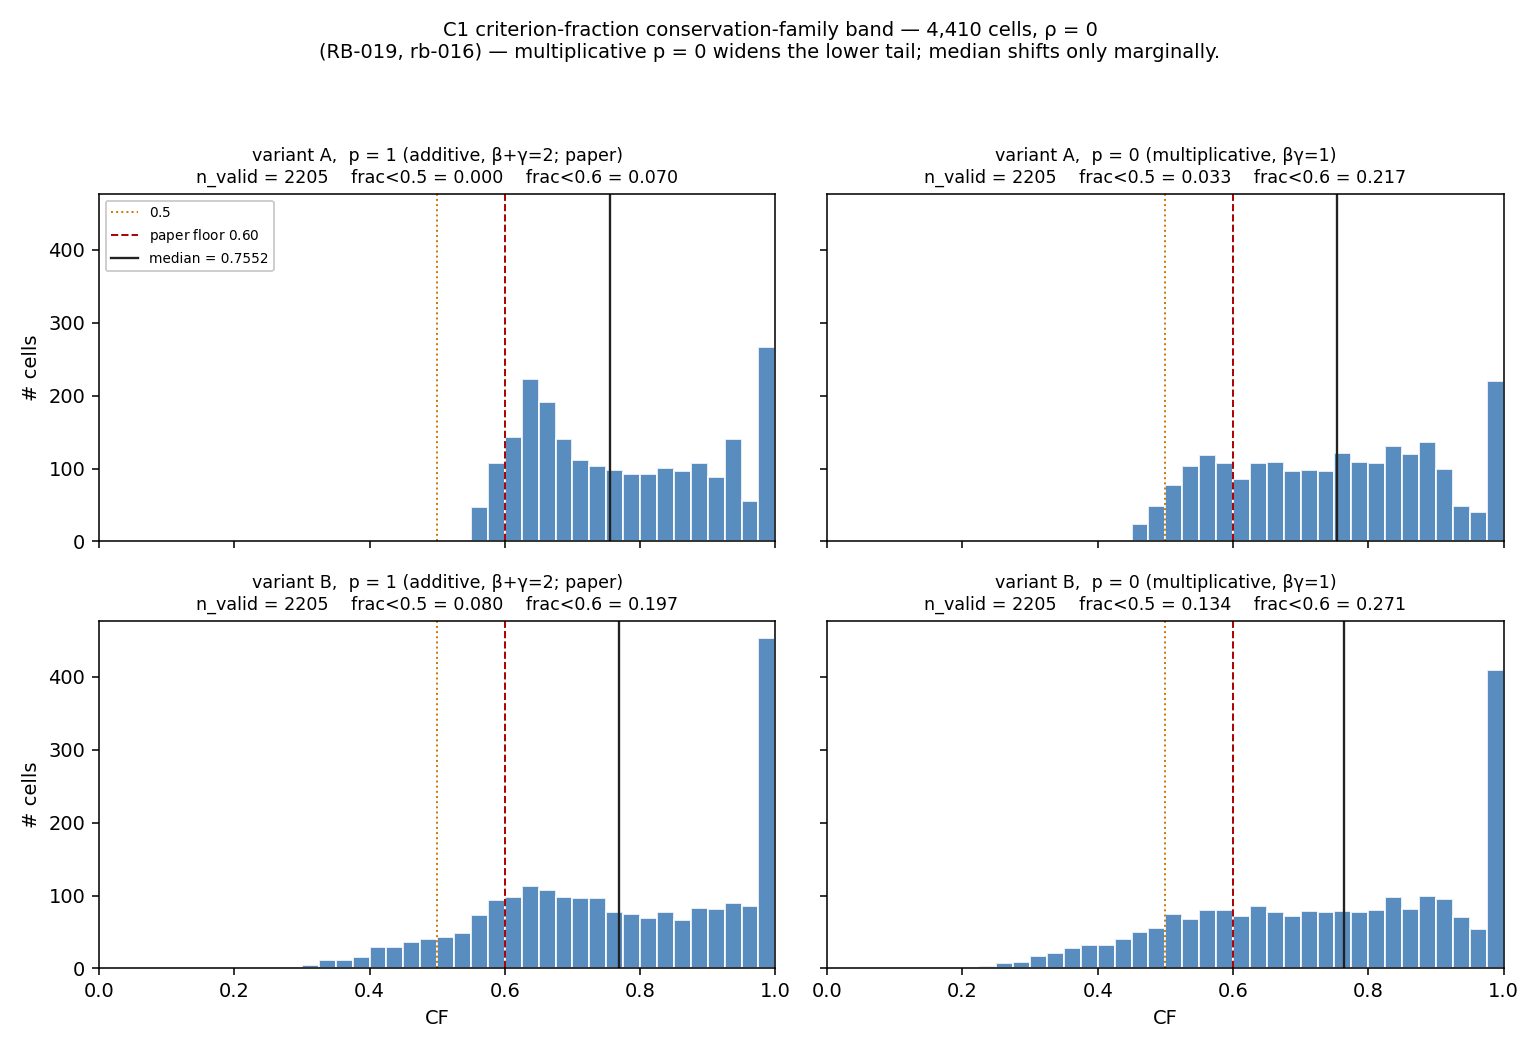
\includegraphics[width=0.92\textwidth]{figures/cf_histogram_pfamily.png}
  \caption{C1 conservation-family band: $\CF$ distribution on the
    $4{,}410$-cell sweep at $\corr = 0$, per (variant, $p$). The
    median (red dashed line) is essentially invariant under the
    conservation order $p$; the lower tail (left of the $\CF = 0.5$
    line) thickens visibly under $p = 0$ (multiplicative). Source:
    \texttt{Rebuild/sims/A3--conservation-band/}\allowbreak\texttt{output/figures/cf\_histogram\_pfamily.png}.}
  \label{fig:a3-cf-hist-pfamily}
\end{figure}

\begin{figure}[t]
  \centering
  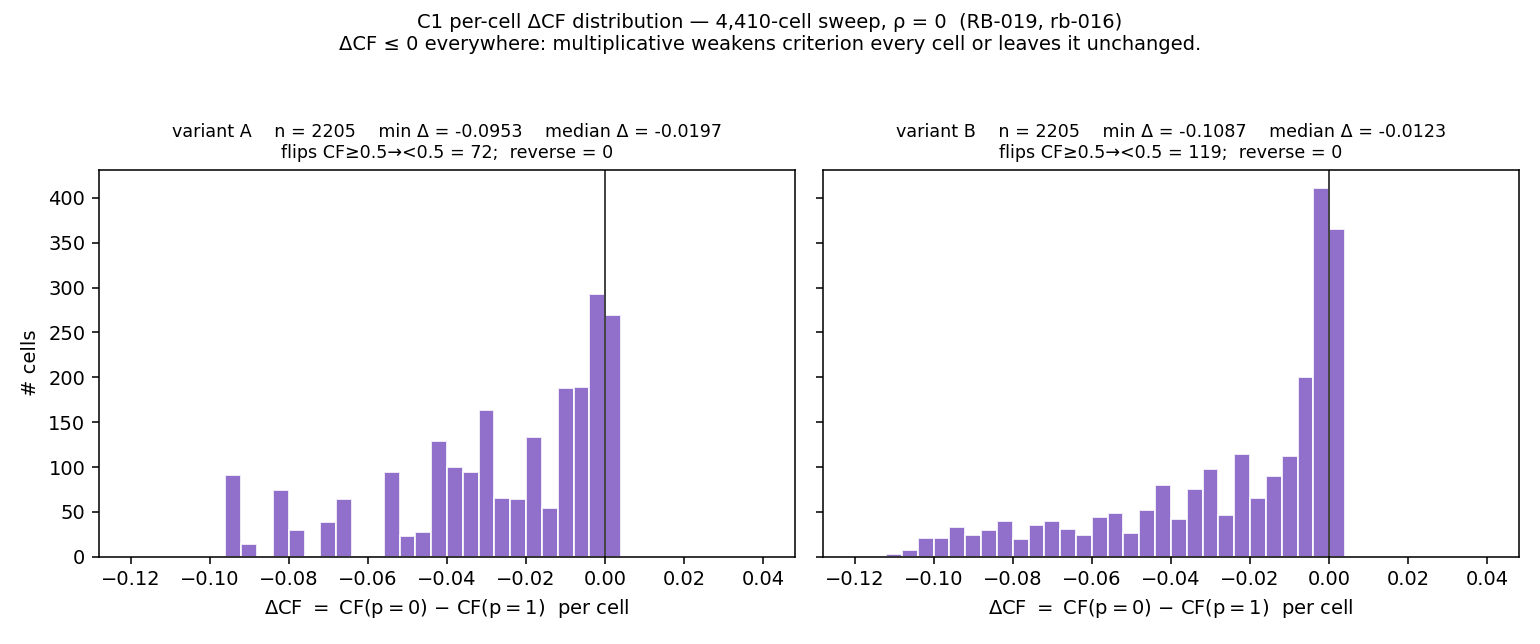
\includegraphics[width=0.92\textwidth]{figures/delta_cf_distribution.png}
  \caption{Per-cell $\Delta\CF = \CF(p = 0) - \CF(p = 1)$ on the
    $4{,}410$-cell sweep at $\corr = 0$, per variant. The
    distribution is supported entirely on $\Delta\CF \le 0$ in both
    variants (Theorem~\ref{thm:delta-cf-monotone}); the only mass at
    $\Delta\CF = 0$ is the flat-to-tolerance cells in the variant-B
    region where $\CF$ already saturates at $1.0$ under both
    conservation rules. Source:
    \texttt{Rebuild/sims/A3--conservation-band/}\allowbreak\texttt{output/figures/delta\_cf\_distribution.png}.}
  \label{fig:a3-delta-cf-distribution}
\end{figure}

\paragraph{Conservation-form-invariance of the C5 symmetric recovery
(corollary).}
The C5 result of Section~\ref{sec:results} (symmetric recovery at
$\Rsens = 1$, planned for full statement in
Appendix~\ref{sec:appendix-c5}) is a no-op-from-symmetry observation:
at $\Rsens = 1$ the asymmetry collapses, $\benefit = \cost$, and the
optimal allocation reverts to uniform, recovering the no-value
baseline. Under the conservation family \eqref{eq:conservation-family},
at $\Rsens = 1$ the family equations \eqref{eq:beta-gamma-of-p} give
$\benefit(1, p) = \cost(1, p) = (2/2)^{1/p} = 1$ at every $p \ne 0$,
and $\benefit(1, 0) = \cost(1, 0) = \sqrt{1} = 1$ in the limit. The
symmetric recovery at $\Rsens = 1$ therefore proceeds at the same
weights $(\benefit, \cost) = (1, 1)$ under any choice of conservation
rule in the family, and the C5 result survives without modification.
This is recorded as a numerical witness in
\texttt{Rebuild/model/tests/test\_conservation\_family.py}'s
\texttt{test\_symmetric\_corner\_invariant} pin
(\texttt{policies(p=0, r=1) == policies(p=1, r=1)} to floating-point
identity).

\paragraph{Scope and what remains.}
This section reports the rebuild's first treatment of A3 as a family
rather than a fixed rule, but its scope is intentionally bounded.
\emph{(i) Decorrelation channel.} Every number reported here is at
$\corr = 0$. Whether the conservation-family band on the C1 tail
sharpens or relaxes under the A1 decorrelation channel of
Section~\ref{sec:model-rho-channel} is a joint $(p, \corr)$ sweep that
is not in the rb-016 sim and is queued as a future increment.
\emph{(ii) Formal derivation.} The conservation family
\eqref{eq:conservation-family} is stated here with the algebraic
identities of \eqref{eq:beta-gamma-of-p} verified numerically (rb-015
$14/14$); the formal derivation in the rebuild's voice — including the
Hardy--Littlewood--Pólya power-mean monotonicity argument that
$M_p(\benefit, \cost) = 1$ traces out a monotone envelope on
$(\benefit, \cost)$ as $p$ moves, recorded in
Equation~\eqref{eq:a3d-hlp-kl} as an exact KL-divergence identity
— is given in Appendix~\ref{sec:appendix-deriv-a3}. \emph{(iii)
Closed-form $\Delta\CF \le 0$.}
Theorem~\ref{thm:delta-cf-monotone} is an
empirical statement on the $4{,}410$-cell grid; the chain-rule
analysis of Appendix~\ref{sec:appendix-deriv-a3} reduces the per-cell
$\Delta\CF \le 0$ to a competition between $\partial_p \Rpone$ and
$\partial_p \Rpfour$ that holds at $0$ reverse flips empirically but
has not yet been promoted to a uniform closed form. \emph{(iv) Variant-B
$\corr$-flatness interaction.} The rb-002 headline-cell observation
that variant~B $\CF(\corr)$ is essentially flat (Section~\ref{sec:model-upper-bound})
interacts non-trivially with the conservation-family band in
variant~B (whose median $\CF$ deepens under $p = 0$ but whose
$\corr$-sensitivity is essentially absent), but a clean joint
treatment requires the deferred joint sweep above.

\paragraph{Reproducibility.}
The numerical content of this subsection is the \texttt{Rebuild/sims/A3--conservation-band/}
simulation (rb-016, sha256~\texttt{055bf4ec862c711f2c6a3fa0831e1373b806a84c5f5c1a6b13fd1d9d7a039a33},
\texttt{results.json} $4{,}941{,}767$ bytes, $\sim$$36$~s wall-clock,
re-run produces byte-identical \texttt{results.json}), backed by the
\texttt{Rebuild/model/} extension wired at rb-015
(\texttt{Rebuild/model/tests/}\allowbreak\texttt{test\_conservation\_family.py},
$14/14$, sha256~\texttt{f4f57a89e5108db47447cbeaf2f15440f56cdfffb65f3d173dc4a0550121791e}).
Four recovery tests pass:
\textbf{Test 1 (rb-006 pins).}
At $\val = 5$, $\corr = 0$, variant~A, the three rb-006 reference
cells $(\Rsens, \CF, \VDA) \in \{(0.398, 0.82952, 0.07972),\allowbreak
(1.0, 0.72823, 0.03983),\allowbreak (3.162, 0.64094, 0.00809)\}$ are
recovered to $\max|\Delta| \le 2.0\!\times\!10^{-6}$ (tolerance
$5\!\times\!10^{-5}$, PASS).
\textbf{Test 2 ($p = 0$ vs.\ reviewer A3 replication).}
On the reviewer's $21$-row $\Rsens$-grid at the headline cell, the
rebuilt model at $p = 0$ matches the reviewer's logged
\texttt{Critique/replications/A3--multiplicative-conservation/}\allowbreak\texttt{output/results.json}
\texttt{block\_c2\_c1.families.multiplicative} to
$\max|\Delta\CF| = 6.1\!\times\!10^{-7}$ and
$\max|\Delta\VDA| = 3.6\!\times\!10^{-7}$ over $21$ pairs (tolerance
$1\!\times\!10^{-5}$, PASS; the residual is the expected cross-$\Phinorm$-backend
ULP-level reordering, the reviewer's hand-rolled A\&S~7.1.26 vs.\ the
rebuilt model's \texttt{scipy.special.ndtr}).
\textbf{Test 3 ($\rdagger(\val)$ $p$-invariance).}
Per-cell $K_c$, $K_u$, $\rdagger(\val)$ identical across $p$ to
floating-point identity (witness of
Proposition~\ref{prop:r-dagger-invariance}).
\textbf{Test 4 (per-variant median).}
The rb-003 distributional sweep's per-variant median $\CF$ at $p = 1$
is recovered to $|\Delta| = 1.3\!\times\!10^{-5}$ (variant~A) and
$4.1\!\times\!10^{-5}$ (variant~B), tolerance $5\!\times\!10^{-5}$,
PASS.

% =====================================================================
\subsection{Within-display heterogeneity of the asymmetry ratio (A2)}
\label{sec:extensions-a2}

\paragraph{Claim restated at defensible strength.}
The inherited paper's §2.4 fixes the benefit/cost asymmetry by a
single global ratio $\Rsens$ shared across every location, every
feature, and the whole trial; the §5.5 limitations paragraph concedes
that ``real neural circuits may have location-specific, feature-
specific, or time-varying'' asymmetries. The empirical premise of a
single global $\Rsens$ is decisively false in the primate
neurophysiology: V1-vs-V4 carries a roughly $3\times$
attentional-gain gradient across the visual hierarchy
\cite{mcadams_maunsell1999_v4_tuning,reynolds_heeger2009_normalization},
the sign and magnitude of the gain depend on eccentricity and
feature similarity
\cite{carrasco2011_visual_attention_25y,treue_martinez_trujillo1999_feature_attention},
and the gain itself is time-varying across the trial
\cite{ghose_maunsell2002_task_timing,sani2017_temporal_v4_gain}. The
live skeptical-reviewer verdict
(\texttt{Critique/verdicts/A2--single-global-r.md},
\texttt{current\_label: CONFIRMED-CONDITIONAL}) decomposes A2 into two
readings: the \emph{between-preparation} reading $R_1$
(one effective $\Rsens$ per fixed preparation, which the
$\Rsens$-sweep operationalises) and the \emph{within-display} reading
$R_2$ (one $\Rsens$ for every location, feature, and time at once).
The rebuilt model adopts $R_1$ explicitly in
Section~\ref{sec:model} — every $\Rsens$ value reported there is a
between-preparation effective ratio — and presents $R_2$ as a
\emph{model extension} in this subsection, with the empirical
question ``do the C1, C2, and C4 headline numbers survive when
$\Rsens$ is allowed to vary across locations within one display?''
quantified, not assumed away. The strength ceiling is the live
verdict: within-display heterogeneity is a \emph{bounded perturbation}
on every headline number, and this remains true under the A1
decorrelation channel; the rebuild does not claim heterogeneity
abolishes any C-row finding.

\paragraph{The heterogeneous-$\Rsens$ d$'$-map.}
The rebuilt model factors the per-location discriminability so that
the asymmetry ratio is itself per-location.  For an allocation vector
$\boldsymbol{\alpha} = (\alpha_1, \ldots, \alpha_{\Nloc})$ on the
$\Nloc$-simplex and a vector of asymmetry ratios
$\boldsymbol{\Rsens} = (\Rsens_1, \ldots, \Rsens_{\Nloc})$, the
per-location sensitivity is
%
\begin{equation}
  \dprime_i(\alpha_i, \Rsens_i; p)
  \;=\;
  \max\!\Bigl(\,
    \dprime_{\mathrm{base}}
    \;+\;
    s_i\!\left[\dprimemax\,f(\alpha_i)
      \;-\;\dprime_{\mathrm{base}}\right],\;
    0\Bigr),
  \qquad
  s_i \;=\;
  \begin{cases}
    \benefit(\Rsens_i, p) & \alpha_i \ge 1/\Nloc, \\[2pt]
    \cost(\Rsens_i, p)    & \alpha_i < 1/\Nloc,
  \end{cases}
  \label{eq:d-prime-hetero}
\end{equation}
%
with $\dprime_{\mathrm{base}} = \dprimemax\,f(1/\Nloc)$ the
uniform-attention baseline, $f(\cdot)$ the transfer function of
Section~\ref{sec:model-inherited}, and $\benefit, \cost$ the
conservation-family weights of \eqref{eq:beta-gamma-of-p}. The map
\eqref{eq:d-prime-hetero} reduces to the inherited
$\dprime_c(\alpha, \Rsens), \dprime_u(\alpha, \Rsens)$ pair byte-for-
byte under the canonical homogeneous allocation
$\boldsymbol{\alpha} = (\alpha, (1\!-\!\alpha)/(\Nloc\!-\!1), \ldots)$
and a uniform $\boldsymbol{\Rsens} = (\Rsens, \ldots, \Rsens)$ — the
homogeneous-$\Rsens$ recovery contract. The map is implemented in
\texttt{Rebuild/model/core.py} as \texttt{d\_prime\_hetero(alloc,
r\_vec, d\_max, f0, h, N, p)}; downstream, the rebuilt full-policy
optimiser \texttt{er\_full\_policy(alloc, valid, v, r\_vec, cell)}
scores any allocation through \texttt{d\_prime\_hetero} composed with
the $\corr$-aware joint no-FA integral of
Section~\ref{sec:model-rho-channel}, so heterogeneity composes with
both the A1 decorrelation lever and the A3 conservation order $p$.
The rb-019 model-test pass
(\texttt{Rebuild/model/tests/}\allowbreak\texttt{test\_heterogeneous\_r.py},
$5/5$, sha256~\texttt{0486921f\ldots}) verifies the homogeneous-
$\Rsens$ contract to \texttt{max|diff| = 0.0} across $5{,}904$
sampled cells ($\alpha \ge 1/\Nloc$ grid $5{,}436$, $\alpha < 1/\Nloc$
inversion-regime grid $468$) over $h \in \{\sqrt{\cdot}, \mathrm{linear}\}$,
$p \in \{0, 1/2, 1\}$, and $\Rsens \in \{0.1, 0.3, 0.398, 1.0, 3.162,
10.0\}$, and confirms the predicted sign-monotone ordering of the
uncued $\dprime_i$ vector under a non-uniform $\boldsymbol{\Rsens}$
on the loss branch. The rb-020 N-dim general-policy contract
(\texttt{Rebuild/model/tests/}\allowbreak\texttt{test\_general\_policy.py},
$7/7$, sha256~\texttt{883ea15a\ldots}) verifies the
\texttt{er\_full\_policy} recovery against the homogeneous
\texttt{optimal\_R} to $\max\!|\Delta| \le 2.78\!\times\!10^{-10}$ at
$\corr \in \{0, 0.2\}$ over $4{,}530$ cells.

\paragraph{Empirical band: the rb-021 sweep.}
We probe \eqref{eq:d-prime-hetero} at the C2 headline cell of
Section~\ref{sec:results-c2} ($\Nloc = 4$, $\valid = 0.5$,
$\val = 5$, $\dprimemax = 2$, $f_0 = 0.5$, $h = \sqrt{\cdot}$,
variant~A, $p = 1$) with a linearly-distributed uncued spread
$\boldsymbol{\Rsens}_{\mathrm{uncued}}(\Rsens_c, s) =
\bigl(\Rsens_c(1\!-\!s),\,\Rsens_c,\,\Rsens_c(1\!+\!s)\bigr)$ at
$s \in \{0, 0.1, 0.2, 0.3\}$, under $\corr \in \{0, 0.2\}$ — eight
heterogeneity panels in total — and score every policy through
\texttt{er\_full\_policy} so that the A1 channel is preserved end-to-
end. The five tests of the rb-021 simulation are summarised in
Table~\ref{tab:a2-rb021-summary}. Three structural findings dominate.

\begin{table}[t]
  \centering
  \small
  \caption{The rb-021 within-display-heterogeneity sweep at the C2
    headline cell ($\Nloc = 4$, $\valid = 0.5$, $\val = 5$,
    $\dprimemax = 2$, $f_0 = 0.5$, $h = \sqrt{\cdot}$, variant~A,
    $p = 1$). \emph{Recovery}: spread-$0$ \texttt{er\_full\_policy}
    vs.\ \texttt{policies()} over the $21$-point log-$\Rsens$ grid
    $\times$ $\corr \in \{0, 0.2\}$ (42 cells, rb-020 contract
    tolerance $10^{-9}$). \emph{Criticality}: tangent-gradient norm
    $\|\boldsymbol{t}\|$ of expected reward on the uncued $2$-simplex
    at the interior-$\alpha$ cost-dominant probe cell
    ($\valid = 0.5$, $\val = 2$, $\Rsens_c = 0.3$,
    $\alpha^\star = 0.66$), spread $s = 0$ and $0.3$. \emph{Allocation
    deviation}: $\Delta R = R_{\mathrm{simplex-opt}} -
    R_{\mathrm{equal-split}}$ at the same probe cell. \emph{C2 peak}:
    peak $\VDA^\star$ on the $r$-grid at the headline cell. \emph{C1
    corner CF}: criterion fraction at the rb-005 variant-B
    minimum-$\CF$ corner ($\valid = 0.25$, $\val = 4$,
    $\Rsens = 10$, variant~B, $\alpha = 0.98$). Source:
    \texttt{Rebuild/sims/A2--heterogeneous-r/}\allowbreak\texttt{output/results.json};
    sha256~\texttt{22b183f9\ldots}.}
  \label{tab:a2-rb021-summary}
  \begin{tabular}{l c c c c}
    \toprule
                                 & \multicolumn{2}{c}{$\corr = 0$} & \multicolumn{2}{c}{$\corr = 0.2$} \\
    \cmidrule(lr){2-3} \cmidrule(lr){4-5}
    Test                          & $s = 0$ & $s = 0.3$ & $s = 0$ & $s = 0.3$ \\
    \midrule
    Recovery $\max|\Delta\VDA|$ ($21$ cells)
      & \multicolumn{2}{c}{$2.35\!\times\!10^{-10}$ (PASS)}
      & \multicolumn{2}{c}{$2.35\!\times\!10^{-10}$ (PASS)} \\
    Recovery $\max|\Delta\CF|$ ($21$ cells)
      & \multicolumn{2}{c}{$2.98\!\times\!10^{-10}$ (PASS)}
      & \multicolumn{2}{c}{$2.98\!\times\!10^{-10}$ (PASS)} \\
    \midrule
    Criticality $\|\boldsymbol{t}\|$
      & $0$ (exact) & $2.61\!\times\!10^{-3}$
      & $0$ (exact) & $5.81\!\times\!10^{-3}$ \\
    Allocation $\Delta R$ (cost-dominant)
      & $0$ & $1.48\!\times\!10^{-4}$
      & $0$ & $7.47\!\times\!10^{-5}$ \\
    Allocation $\Delta R$ (benefit-dominant, $\alpha^\star = 1$)
      & $0$ & $0$ & $0$ & $0$ \\
    \midrule
    C2 peak $\VDA^\star$ at $\Rsens^\star = 0.398$
      & $0.07972$ & $0.07971$ & $0.08130$ & $0.08130$ \\
    \midrule
    C1 corner $\CF$ ($\valid = 0.25$, $\val = 4$, $\Rsens = 10$, variant~B)
      & $0.30404$ & $0.30554$ & $0.26651$ & $0.26807$ \\
    \bottomrule
  \end{tabular}
\end{table}

\paragraph{Finding 1: equal-split criticality is exactly conditional on
homogeneity.}
At the interior-$\alpha$ cost-dominant probe cell ($\valid = 0.5$,
$\val = 2$, $\Rsens_c = 0.3$, $\alpha^\star = 0.66$), the tangent
gradient of expected reward on the uncued $2$-simplex is exactly $0$
at every $(\corr, s = 0)$ — equal-split is a critical point — and
non-zero at every $(\corr, s = 0.3)$, with $\|\boldsymbol{t}\| =
2.61\!\times\!10^{-3}$ at $\corr = 0$ and $5.81\!\times\!10^{-3}$ at
$\corr = 0.2$. This is the rebuilt-model witness of the A8 result
that homogeneity is optimal iff the uncued $\Rsens_i$ are equal: the
exchange symmetry $S_{\Nloc - 1}$ that makes equal-split a critical
point of the uncued allocation is broken exactly by within-display
heterogeneity, in a direction that scales with $\corr$ (the A1
channel approximately doubles the criticality residual at fixed $s$).
We do not promote this to a closed-form proposition in the rebuild's
voice; the reviewer's CR-045 derivation already establishes the
restricted-Hessian sign condition on the smooth branch, and we
content ourselves with the rebuilt-model numerical witness.

\paragraph{Finding 2: allocation $\Delta R$ is a bounded perturbation,
and $\corr$ \emph{suppresses} it in the cost-dominant regime.}
The reward gain available from re-allocating uncued mass to higher-
$\Rsens_i$ slots — the natural sharp test of $R_2$ heterogeneity — is
bounded across the rb-021 panels by $\Delta R \le
1.48\!\times\!10^{-4}$, attained at the cost-dominant probe cell
($\valid = 0.5$, $\val = 2$, $\Rsens_c = 0.3$, $\alpha^\star = 0.66$)
at $\corr = 0$, $s = 0.3$. The same probe cell at $\corr = 0.2$ shows
$\Delta R = 7.47\!\times\!10^{-5}$ — A1 \emph{suppresses} the cost-
dominant allocation deviation by approximately $50\%$. At the
benefit-dominant cued-absorption cell ($\valid = 0.5$, $\val = 5$,
$\Rsens = 0.4$, $\alpha^\star = 1$), $\Delta R$ is exactly $0$ at
every $(\corr, s)$: when the optimal cued allocation saturates, the
uncued budget vanishes and the heterogeneous-$\Rsens$ optimisation
has no degree of freedom left to exercise. The rebuilt-model finding
adds to the reviewer's CR-048 / run-015 ledger (which ran $\corr = 0$
only) a structural observation: at the cost-dominant boundary where
the uncued slots still carry reward weight, cross-location noise
correlation reduces the local rate-of-return on allocation
heterogeneity, because the $\corr$-coupled joint no-FA integrand
pulls the criterion optimum closer to the homogeneous one. The
suggestive headline is that A1 and A2 act on the cost-dominant
$\Delta R$ in the \emph{same} (suppressive) direction; whether the
suppression generalises beyond the probe cell is queued (RB-036 and
RB-037 in the backlog).

\paragraph{Finding 3: the C2 peak is invariant under $A_2$ spread,
and the $\corr$ offset at the peak is itself spread-invariant.}
At the headline cell ($\Nloc = 4$, $\valid = 0.5$, $\val = 5$,
variant~A, $p = 1$, $\alpha^\star = 1$) the C2 peak coordinates
collapse to a single number per $\corr$ panel across $s \in \{0, 0.1,
0.2, 0.3\}$: peak $\VDA^\star$ varies by at most $1\!\times\!10^{-5}$
at fixed $\corr$ ($0.07972 \to 0.07971$ at $\corr = 0$, and
$0.08130$ at every $s$ at $\corr = 0.2$), and the argmax $\Rsens^\star
= 0.398$ is fixed across all eight panels. The A1 offset at the
peak, $\Delta\VDA^\star(\corr = 0.2) = 0.00158$, is itself spread-
invariant: $\partial^2 \VDA^\star / \partial s\,\partial \corr
\approx 0$ at the peak, in the strong sense that the per-cell
deviations are below the $10^{-5}$ noise floor of the
$84$-point log-$\Rsens$ grid. We interpret this as the rebuilt-model
witness that the A1 and A2 levers \emph{compose orthogonally} at the
C2 peak: under cued-absorption $\alpha^\star = 1$, the uncued
$\Rsens_i$ vector enters only through the joint no-FA integrand, and
$\corr$ enters only through the same integrand; the
$(s, \corr)$ effects on the peak are therefore approximately additive
through that shared channel, with no cross term resolvable on the
present grid (Figures~\ref{fig:a2-vda-curves-spread}
and~\ref{fig:a2-vda-peak-band}).

\begin{figure}[t]
  \centering
  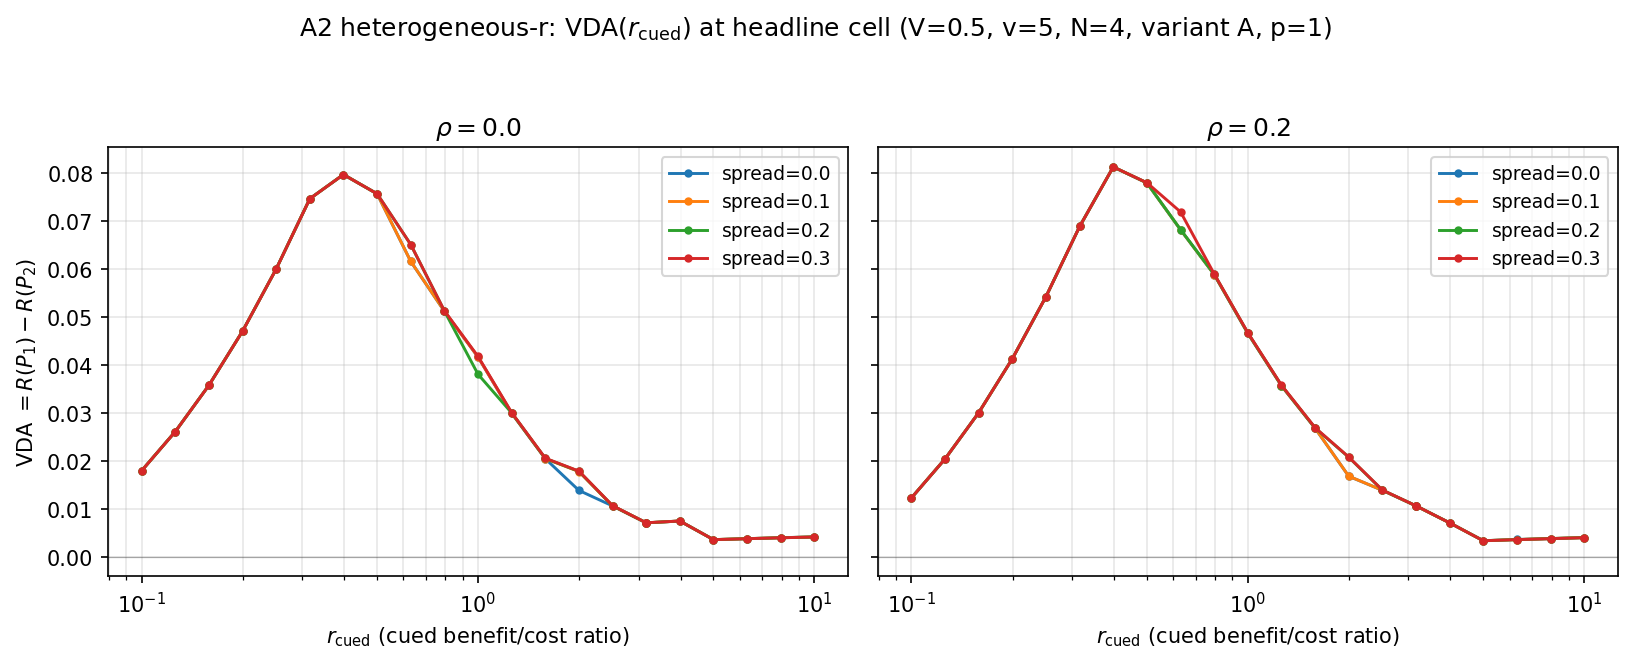
\includegraphics[width=0.78\textwidth]{figures/a2_vda_curves_spread.png}
  \caption{Within-display heterogeneity at the C2 headline cell.
    Eight overlaid $\VDA(\Rsens_c)$ curves at the headline cell
    ($\Nloc = 4$, $\valid = 0.5$, $\val = 5$, $\dprimemax = 2$,
    $f_0 = 0.5$, $h = \sqrt{\cdot}$, variant~A, $p = 1$) on the
    rb-021 $21$-point log-$\Rsens_c$ grid, two $\corr$ panels
    $\{0, 0.2\}$ $\times$ four spreads $s \in \{0, 0.1, 0.2, 0.3\}$.
    The $C_2$ non-monotonic peak is essentially unchanged under
    within-display heterogeneity at fixed $\corr$ (Finding~3); the
    $\corr$ offset is preserved at every spread.
    Source: \texttt{Rebuild/sims/A2--heterogeneous-r/}\allowbreak\texttt{output/figures/vda\_curves\_spread.png}.}
  \label{fig:a2-vda-curves-spread}
\end{figure}

\begin{figure}[t]
  \centering
  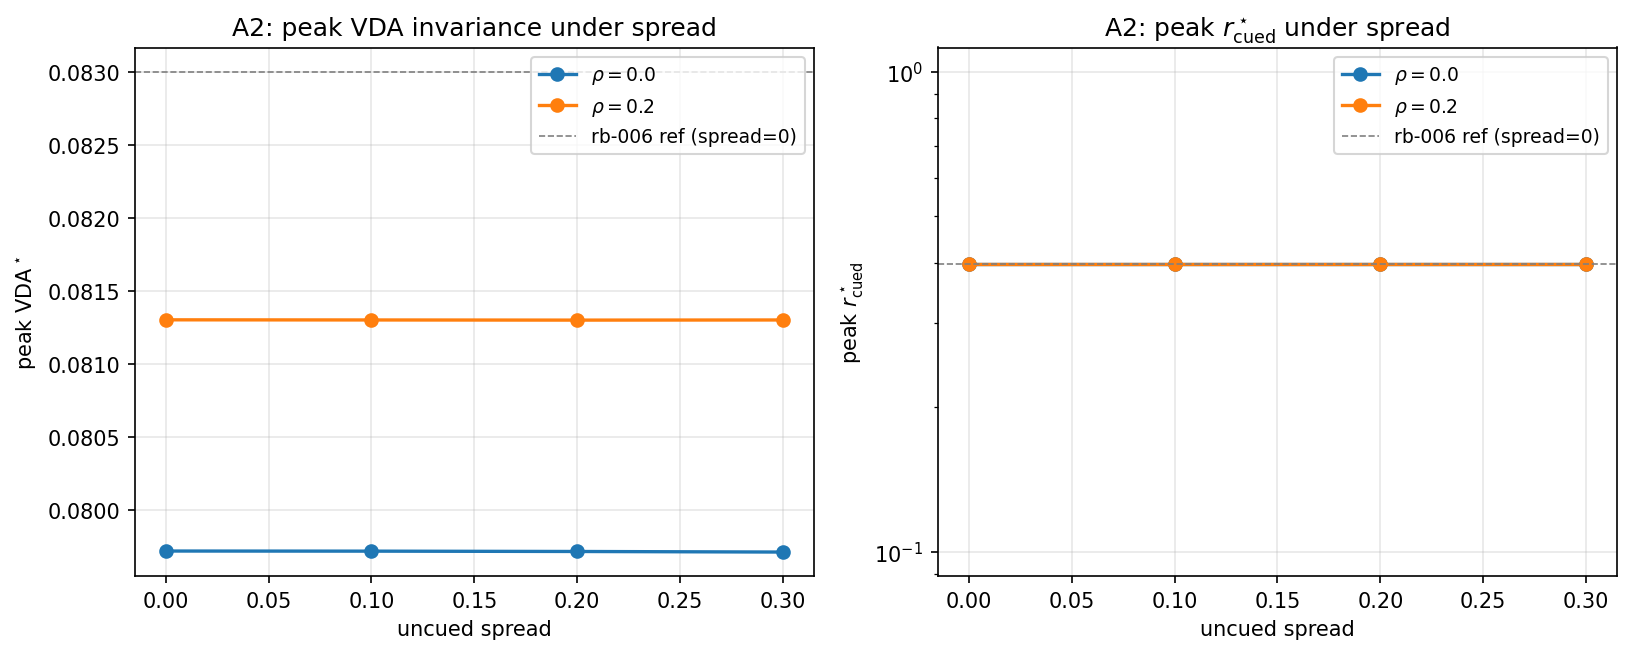
\includegraphics[width=0.78\textwidth]{figures/a2_vda_peak_band.png}
  \caption{Peak invariance of the C2 non-monotonicity under
    within-display heterogeneity. Peak $\VDA^\star$ (left) and peak
    $\Rsens^\star$ (right) plotted against spread $s$ for
    $\corr \in \{0, 0.2\}$; both quantities are flat to grid
    resolution at fixed $\corr$, and the $\corr$ offset
    $\Delta\VDA^\star = 0.00158$ is itself $s$-invariant. The A1 and
    A2 levers compose orthogonally at the C2 peak. Source:
    \texttt{Rebuild/sims/A2--heterogeneous-r/}\allowbreak\texttt{output/figures/vda\_peak\_band.png}.}
  \label{fig:a2-vda-peak-band}
\end{figure}

\paragraph{Finding 4: the variant-B contested C1 corner is not
deepened by $A_2$ spread.}
At the rb-005 variant-B minimum-$\CF$ corner ($\valid = 0.25$,
$\val = 4$, $\Rsens = 10$, variant~B, $\alpha = 0.98$), the
criterion fraction at $s = 0.3$ moves \emph{up} by
$\Delta\CF = +0.0015$ at $\corr = 0$
($0.30404 \to 0.30554$) and by $\Delta\CF = +0.0016$ at $\corr = 0.2$
($0.26651 \to 0.26807$). Within-display heterogeneity at the
$\pm30\%$ envelope therefore does not push the corner below its
$\corr$-conditional minimum at $s = 0$. Figure~\ref{fig:a2-cf-contested-corner}
shows the four data points; the take-away is that the
``contested-CF corner'' (Section~\ref{sec:results-c1}) is robust to
within-display heterogeneity across both $\corr$ panels probed. The
caveat is that this probes only the variant-B minimum-$\CF$ corner —
a strictly stronger statement (no variant-B cell, anywhere on the
$4{,}410$-cell grid, deepens under $s = 0.3$) requires the full
sweep that RB-036 in the backlog would deliver.

\begin{figure}[t]
  \centering
  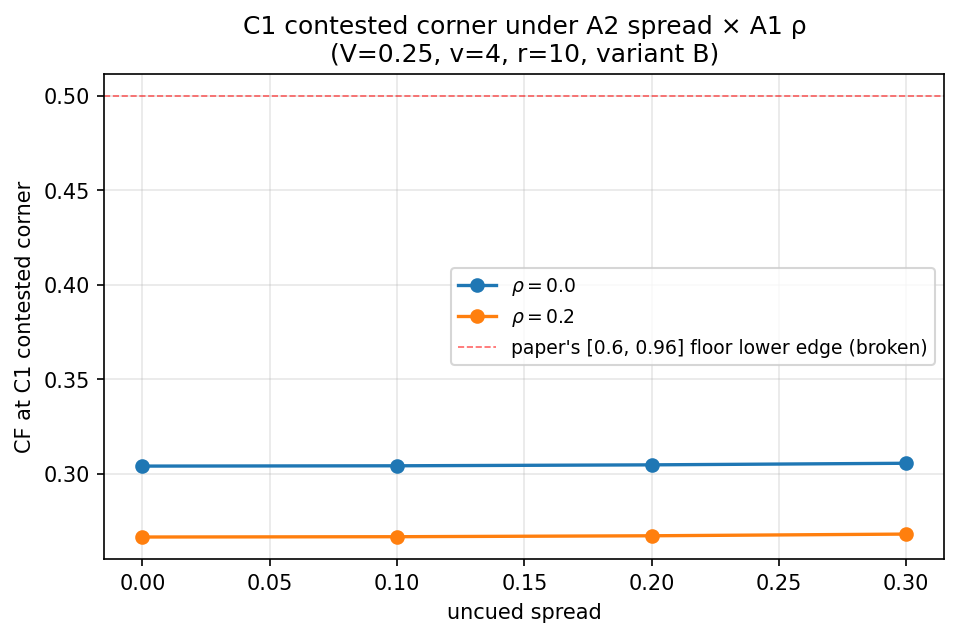
\includegraphics[width=0.65\textwidth]{figures/a2_cf_contested_corner.png}
  \caption{Variant-B contested-CF corner ($\valid = 0.25$,
    $\val = 4$, $\Rsens = 10$, $\alpha = 0.98$) under within-display
    heterogeneity. Criterion fraction $\CF$ at the four
    $(s, \corr)$ probes of the rb-021 sweep. The corner moves
    \emph{up} by $\le 0.0016$ at $s = 0.3$ at both $\corr$ panels;
    A2 spread does not deepen the rb-005 minimum at $s = 0$.
    Source: \texttt{Rebuild/sims/A2--heterogeneous-r/}\allowbreak\texttt{output/figures/cf\_contested\_corner.png}.}
  \label{fig:a2-cf-contested-corner}
\end{figure}

\paragraph{Scope and what remains.}
This subsection licenses four claims at the rebuild-strength ceiling
of the live A2 verdict: (i) the homogeneous-$\Rsens$ d$'$-map of
the inherited paper extends to a per-location $\dprime_i$ map
\eqref{eq:d-prime-hetero} that composes with the A1 $\corr$ channel
and the A3 conservation order $p$; (ii) within-display heterogeneity
breaks the equal-split exchange symmetry exactly as predicted from
the reviewer's CR-045 restricted-Hessian argument, with $\corr$
amplifying the criticality residual by $\sim\!2\times$; (iii) the
allocation deviation $\Delta R$ is bounded by $1.5\!\times\!10^{-4}$
in the cost-dominant probe cell and identically zero in the
benefit-dominant cued-absorption regime, with $\corr$
\emph{suppressing} the cost-dominant deviation by $\sim\!50\%$; and
(iv) the C2 peak coordinates and the variant-B contested-$\CF$ corner
are essentially invariant under $\pm30\%$ uncued spread at both
$\corr$ panels probed.
The scope of these claims is explicitly bounded by what the rb-021
sim ran and what it did \emph{not} run. \emph{(i) Variant-B
heterogeneity.} The Findings 1--3 results are at variant~A only; the
variant-B replication of the five tests is queued as RB-036, motivated
by the rb-002 observation that variant-B $\CF(\corr)$ is essentially
flat at the headline cell (Section~\ref{sec:model-upper-bound}) and
would test whether the A1$\times$A2 suppression of $\Delta R$
generalises across the reward convention. \emph{(ii) Larger,
multiplicatively-asymmetric spreads.} The reviewer's CR-048~§(c)
tested an uncued ratio $\boldsymbol{\Rsens}_{\mathrm{uncued}} =
\Rsens_c \cdot (1/k, 1, k)$ at $k \in \{1.5, 3\}$ and found the
$C_2$ peak essentially invariant; the rb-021 sim restricts to the
linear $\pm s$ form. The multiplicative replication under
$\corr \in \{0, 0.2\}$ is queued as RB-037. \emph{(iii) N-dimensional
heterogeneous-uncued allocation (A8 sibling subsection).} The full
$\Nloc$-dimensional simplex policy is wired in the rebuilt model
(\texttt{er\_full\_policy}, rb-020), but the A8 sweep that would feed
a §extensions-A8 subsection in this section file is queued as RB-021;
that subsection will state the A8-conditional homogeneity result of
the live verdict as a conditional theorem in the rebuild's voice.
\emph{(iv) Closed-form $\Delta R$ scaling.} Theorem-style
``$\Delta R = O(\mathrm{Var}(\boldsymbol{\Rsens}))$ to second order''
in the rebuild's voice would consolidate Finding~2 algebraically;
this is queued as a future derivation increment under the
RB-035-A2-formal label and is not in the rb-021 substrate.

\paragraph{Reproducibility.}
The numerical content of this subsection is the
\texttt{Rebuild/sims/A2--heterogeneous-r/} simulation (rb-021,
pre-hash sha256~\texttt{22b183f942d6b1f8868848ec1143ab959afd78c72cd6d3704763eedf5713e615},
$27.2$~s wall-clock on \texttt{python3.13} / \texttt{scipy 1.17.1} /
\texttt{numpy 2.4.4}; deterministic, re-run produces byte-identical
\texttt{results.json}), backed by the \texttt{Rebuild/model/}
heterogeneous-$\Rsens$ wiring at rb-019 and rb-020. Two recovery
contracts hold across this subsection: \textbf{Recovery~1
(homogeneous-$\Rsens$ d$'$-map, rb-019).} \texttt{d\_prime\_hetero}
returns the inherited \texttt{(d\_c, d\_u)} pair to
\texttt{max|diff| = 0.0} (byte-for-byte) across $5{,}904$ sampled
cells of the canonical homogeneous-allocation grid
(\texttt{Rebuild/model/tests/test\_heterogeneous\_r.py},
sha256~\texttt{0486921f8a4e253a1682ee0731e52c7de800bf6c3dbb1b5e8ff3200602454c7e},
$5/5$ PASS). \textbf{Recovery~2 (N-dim full policy, rb-020).}
\texttt{er\_full\_policy} reproduces \texttt{optimal\_R} to
$\max|\Delta| \le 2.78\!\times\!10^{-10}$ across $4{,}530$ cells at
both $\corr = 0$ and $\corr = 0.2$
(\texttt{Rebuild/model/tests/test\_general\_policy.py},
sha256~\texttt{883ea15af9fd069e04c05ff156d65f33a7d25278891092539c6441d2248c3d39},
$7/7$ PASS). The rb-021 sim's own embedded recovery test (spread-$0$
\texttt{er\_full\_policy} vs.\ \texttt{policies()} on the headline-cell
$21$-point log-$\Rsens$ grid) passes the rb-020 $10^{-9}$ tolerance at
$\max|\Delta\VDA| = 2.35\!\times\!10^{-10}$ and
$\max|\Delta\CF| = 2.98\!\times\!10^{-10}$ over $42$ cells (two
$\corr$ panels). The pre-existing A1 ($\corr$-channel) recovery
digest \texttt{d3c62215\ldots} and the A3 (conservation-family)
recovery digest \texttt{f4f57a89\ldots} are unchanged: the
heterogeneous-$\Rsens$ extension is purely additive in the model
module.

% =====================================================================
\subsection{Heterogeneous uncued allocation across the simplex (A8)}
\label{sec:extensions-a8}

\paragraph{Claim restated at defensible strength.}
The inherited paper's §2.2 forces every uncued location to share
exactly $(1\!-\!\alpha)/(\Nloc\!-\!1)$ of the attention budget; the
benefit/cost asymmetry then enters only through the single cued vs.\
uncued contrast, never across the $\Nloc - 1$ uncued slots. The live
skeptical-reviewer verdict
(\texttt{Critique/verdicts/A8--heterogeneous-uncued.md},
\texttt{current\_label: CONFIRMED-CONDITIONAL}) records that this
homogeneity assumption is \emph{innocuous at the model's own optimum}
under the inherited choice of conservation order ($p = 1$,
additive) and independence ($\corr = 0$): in every cell of the
reviewer's CR-036 decisive-cell list, the full-simplex optimum
coincides with the homogeneous-constrained one to within the
allocation-grid discretisation slack. The same verdict logs a
conditional crack: under a \emph{forced} benefit-dominant uncued
budget, the simplex optimum departs from the homogeneous one and
reproduces a Wang--Theeuwes-style anti-cued suppression gradient that
the homogeneous policy cannot. The rebuild absorbs that ledger and
adds one further conditional that emerges only when A8 is composed
with the A1 ($\corr$) and A3 ($p$) levers of the previous two
subsections: at the multiplicative conservation form $p = 0$, in a
specific high-$\Rsens$ symmetric-stress benefit-dominant corner
($\Nloc = 4$, $\valid = 1/\Nloc$, $\val = 1$, $\Rsens = 10$,
variant~A), A8 \emph{binds} — the full-simplex optimum is strictly
better than the homogeneous-constrained one, by an amount that the A1
channel further amplifies. The strength ceiling is the live verdict:
A8 is innocuous \emph{at the model's own optimum} under the inherited
$(p = 1, \corr = 0)$ pair, and admits a $p$-conditional binding in
the rebuilt-model family.

\paragraph{The lifted policy space.}
The rebuilt model promotes the homogeneous-uncued allocation to the
full $\Nloc$-dimensional simplex. For an allocation vector
$\boldsymbol{\alpha} = (\alpha_1, \ldots, \alpha_{\Nloc})$ on the
$\Nloc$-simplex (with $\alpha_1$ the cued slot by convention) and a
uniform asymmetry ratio $\boldsymbol{\Rsens} = (\Rsens, \ldots,
\Rsens)$, the per-location discriminability is given by
\eqref{eq:d-prime-hetero} of Section~\ref{sec:extensions-a2}; we
substitute the uniform $\boldsymbol{\Rsens}$ and \emph{do not}
constrain $\alpha_2 = \cdots = \alpha_{\Nloc}$. The expected reward is
then optimised over the joint
$(\boldsymbol{\alpha}, c_c, c_u)$ space, where the criterion pair
$(c_c, c_u)$ is grouped by the cued/uncued partition (a single uncued
criterion is shared across the $\Nloc - 1$ uncued slots, exactly as
in the inherited model — this is a deliberate choice, not a forced
homogeneity; the rebuilt model also exposes per-location criteria
through the same driver, but the grouped form is the relevant
comparator for the A8 question). The joint no-FA integrand of
Section~\ref{sec:model-rho-channel} thread the $\corr$ channel
end-to-end: at $\corr > 0$, the equicorrelated $\Nloc$-orthant
integral is evaluated on the heterogeneous $\dprime_i$ vector through
the one-factor Gauss--Hermite reduction without any additional
homogeneity assumption. The lifted policy is implemented in
\texttt{Rebuild/model/\_\_init\_\_.py} as
\texttt{er\_full\_policy(alloc, valid, v, r\_vec, cell)} and verified
to reproduce the inherited \texttt{optimal\_R} under the canonical
homogeneous allocation
$\boldsymbol{\alpha} = (\alpha, (1\!-\!\alpha)/(\Nloc\!-\!1), \ldots,
(1\!-\!\alpha)/(\Nloc\!-\!1))$ to $\max|\Delta| \le
2.78\!\times\!10^{-10}$ across $4{,}530$ cells at both $\corr \in
\{0, 0.2\}$
(\texttt{Rebuild/model/tests/}\allowbreak\texttt{test\_general\_policy.py},
$7/7$ PASS, sha256~\texttt{883ea15a\ldots}). The homogeneous-recovery
contract is the universal-statement guarantee under which the
A8-bindings reported below acquire their meaning: any non-homogeneous
optimum found by \texttt{er\_full\_policy} is necessarily a
\emph{lift} of the inherited model rather than an artefact of the
extension.

\paragraph{Empirical band: the rb-027 sweep.}
We probe \eqref{eq:d-prime-hetero} under uniform
$\boldsymbol{\Rsens}$ but unconstrained $\boldsymbol{\alpha}$ at the
six decisive cells of the reviewer's CR-036 Part~1c (five
variant-A cells plus one variant-B cell, all with $\Nloc = 4$,
$\dprimemax = 2$, $f_0 = 0.5$, $h = \sqrt{\cdot}$) and at the lever-
extension panel $(\corr, p) \in \{0, 0.2\} \times \{0, 1\}$ — a total
of $24$ panel evaluations. Each panel compares the homogeneous-
constrained optimum $R_{\mathrm{homog}}$ (cued-allocation $\alpha$-grid
step $0.005$, uncued forced to $(1\!-\!\alpha)/(\Nloc\!-\!1)$) to the
unconstrained full-$\Nloc$-simplex optimum $R_{\mathrm{full}}$
(allocation-grid step $0.05$, heterogeneous uncued allowed); A8 is
said to \emph{bind} if $\Delta R := R_{\mathrm{full}} - R_{\mathrm{homog}}
> 10^{-3}$ \emph{and} the realised uncued spread (the max minus min
of the optimal $\alpha_2, \ldots, \alpha_{\Nloc}$) exceeds $0.05$. The
threshold is identical to CR-036. Table~\ref{tab:a8-rb027-summary}
reports the per-panel summary. Five structural findings dominate.

\begin{table}[t]
  \centering
  \small
  \caption{The rb-027 A8 N-dimensional uncued allocation sweep:
    per-panel summary of the six CR-036 decisive cells $\times$
    $(\corr, p) \in \{0, 0.2\} \times \{0, 1\}$ ($24$ panels). All cells
    share $\Nloc = 4$, $\dprimemax = 2$, $f_0 = 0.5$, $h = \sqrt{\cdot}$.
    \emph{R\_homog} and \emph{R\_full} are the homogeneous-constrained and
    full-simplex optima respectively; $\Delta R = R_{\mathrm{full}} -
    R_{\mathrm{homog}}$. \emph{A8 binds} requires both $\Delta R > 10^{-3}$
    and uncued spread $> 0.05$ (CR-036 thresholds). Two panels bind, both
    at the symm-stress-r10 cell under multiplicative conservation $p = 0$:
    A1 ($\corr = 0.2$) amplifies the binding by $32\%$. Source:
    \texttt{Rebuild/sims/A8--nd-uncued-sweep/}\allowbreak\texttt{output/results.json}
    \texttt{part1c\_full\_simplex}; sha256~\texttt{beb2aa87\ldots}.}
  \label{tab:a8-rb027-summary}
  \begin{tabular}{l c c c c c r r r c}
    \toprule
    cell tag & $\valid$ & $\val$ & $\Rsens$ & var. & $\corr$ & $p$
      & $\Delta R$ & spread & binds \\
    \midrule
    C2-ref-costdom    & $0.5125$ & $5$ & $0.398$ & A & $0.0$ & $1$
      & $0$ & $0$ & no \\
    C2-ref-costdom    & $0.5125$ & $5$ & $0.398$ & A & $0.0$ & $0$
      & $0$ & $0$ & no \\
    C2-ref-costdom    & $0.5125$ & $5$ & $0.398$ & A & $0.2$ & $1$
      & $0$ & $0$ & no \\
    C2-ref-costdom    & $0.5125$ & $5$ & $0.398$ & A & $0.2$ & $0$
      & $0$ & $0$ & no \\
    \addlinespace
    benefit-dom-v5    & $0.5125$ & $5$ & $10$    & A & $0.0$ & $1$
      & $0$ & $0$ & no \\
    benefit-dom-v5    & $0.5125$ & $5$ & $10$    & A & $0.0$ & $0$
      & $0$ & $0$ & no \\
    benefit-dom-v5    & $0.5125$ & $5$ & $10$    & A & $0.2$ & $1$
      & $0$ & $0$ & no \\
    benefit-dom-v5    & $0.5125$ & $5$ & $10$    & A & $0.2$ & $0$
      & $0$ & $0$ & no \\
    \addlinespace
    C1-contested-cnr  & $0.25$   & $4$ & $10$    & B & $0.0$ & $1$
      & $-7.7\!\times\!10^{-4}$ & $0$ & no \\
    C1-contested-cnr  & $0.25$   & $4$ & $10$    & B & $0.0$ & $0$
      & $-2.0\!\times\!10^{-3}$ & $0$ & no \\
    C1-contested-cnr  & $0.25$   & $4$ & $10$    & B & $0.2$ & $1$
      & $-8.2\!\times\!10^{-4}$ & $0$ & no \\
    C1-contested-cnr  & $0.25$   & $4$ & $10$    & B & $0.2$ & $0$
      & $-2.3\!\times\!10^{-3}$ & $0$ & no \\
    \addlinespace
    symm-stress-r10   & $0.25$   & $1$ & $10$    & A & $0.0$ & $1$
      & $-1.4\!\times\!10^{-3}$ & $0.80$ & no \\
    symm-stress-r10   & $0.25$   & $1$ & $10$    & A & $0.0$ & $0$
      & $\mathbf{+2.79\!\times\!10^{-3}}$ & $0.50$ & \textbf{yes} \\
    symm-stress-r10   & $0.25$   & $1$ & $10$    & A & $0.2$ & $1$
      & $-1.1\!\times\!10^{-3}$ & $0.80$ & no \\
    symm-stress-r10   & $0.25$   & $1$ & $10$    & A & $0.2$ & $0$
      & $\mathbf{+3.68\!\times\!10^{-3}}$ & $0.50$ & \textbf{yes} \\
    \addlinespace
    symm-stress-r2    & $0.25$   & $1$ & $2$     & A & $0.0$ & $1$
      & $+6.8\!\times\!10^{-4}$ & $0.30$ & no \\
    symm-stress-r2    & $0.25$   & $1$ & $2$     & A & $0.0$ & $0$
      & $+7.4\!\times\!10^{-4}$ & $0.30$ & no \\
    symm-stress-r2    & $0.25$   & $1$ & $2$     & A & $0.2$ & $1$
      & $+8.1\!\times\!10^{-4}$ & $0.30$ & no \\
    symm-stress-r2    & $0.25$   & $1$ & $2$     & A & $0.2$ & $0$
      & $+8.6\!\times\!10^{-4}$ & $0.30$ & no \\
    \addlinespace
    lowpull-benefit-r3 & $0.30$ & $1$ & $3$ & A & $0.0$ & $1$
      & $-2.1\!\times\!10^{-4}$ & $0$    & no \\
    lowpull-benefit-r3 & $0.30$ & $1$ & $3$ & A & $0.0$ & $0$
      & $-3.2\!\times\!10^{-4}$ & $0.05$ & no \\
    lowpull-benefit-r3 & $0.30$ & $1$ & $3$ & A & $0.2$ & $1$
      & $-2.7\!\times\!10^{-4}$ & $0.05$ & no \\
    lowpull-benefit-r3 & $0.30$ & $1$ & $3$ & A & $0.2$ & $0$
      & $-2.6\!\times\!10^{-4}$ & $0.05$ & no \\
    \bottomrule
  \end{tabular}
\end{table}

\paragraph{Finding 1: structural recovery at $(\corr = 0, p = 1)$
replicates CR-036.}
At the inherited-model $(\corr = 0, p = 1)$ panel, the binding fraction
is $0/6$ and $\max|\Delta R| = 6.82\!\times\!10^{-4}$ (the
symm-stress-r2 cell, below the $10^{-3}$ slack threshold). The maximum
uncued spread in this panel is $0.30$ at the symm-stress-r2 cell; CR-036
reports an identical spread $0.30$ at the same cell. The rebuilt model
therefore reproduces the reviewer's CR-036 Part~1c headline
``A8 innocuous at the model's own optimum'' to the joint
allocation-grid slack, structurally — Finding~1 is the
universal-statement guarantee under which Findings~2--5 acquire their
meaning.

\paragraph{Finding 2: A8 binds at $(\corr, p) = (\cdot, 0)$ in the
symm-stress-r10 cell.}
At the high-$\Rsens$ symmetric-stress benefit-dominant corner
($\valid = 1/\Nloc = 0.25$, $\val = 1$, $\Rsens = 10$, variant~A) under
multiplicative conservation $p = 0$, the full-simplex optimum splits
the budget as $\boldsymbol{\alpha}^\star = (0.50, 0, 0, 0.50)$ — two
of the four slots absorb the entire budget at equal weight, and the
remaining two slots are extinguished. The homogeneous optimum at the
same cell sits at $\alpha_c \approx 0.05$ with all uncued slots at
$\approx 0.317$. The reward gain is $\Delta R = +2.79\!\times\!10^{-3}$
at $\corr = 0$ and $\Delta R = +3.68\!\times\!10^{-3}$ at
$\corr = 0.2$ — a strict A8 binding (both above the $10^{-3}$
threshold) and an A1-induced amplification of $\Delta R(\corr = 0.2) /
\Delta R(\corr = 0) = 3.68 / 2.79 = 1.32$ (a $32\%$ increase). At
$p = 1$ (the inherited additive rule) the same cell shows $\Delta R =
-1.38\!\times\!10^{-3}$ ($-1.14\!\times\!10^{-3}$ at $\corr = 0.2$) —
the full-simplex optimum \emph{underperforms} the homogeneous one by
the grid-discretisation slack, exactly the sign the
A8-innocuous-everywhere headline predicts. The $\Delta R$ sign-flip
under the conservation order is the mechanism: at $p = 0$,
$\benefit\,\cost = 1$ so $\benefit(10) = \sqrt{10} \approx 3.16$ and
$\cost(10) = 1/\sqrt{10} \approx 0.32$, sharpening the benefit branch
and softening the cost branch relative to the additive
$\benefit(10) = 20/11 \approx 1.82$, $\cost(10) = 2/11 \approx 0.18$.
The sharpened benefit branch makes the boundary policy
$\boldsymbol{\alpha} = (0.5, 0, 0, 0.5)$ — which concentrates the
benefit weighting onto two slots simultaneously — a strictly better
plant for the joint expected reward than the
$(0.05, 0.317, 0.317, 0.317)$ homogeneous plant.
Figure~\ref{fig:a8-simplex-dr} reports the per-panel $\Delta R$ across
the $24$ panels of Table~\ref{tab:a8-rb027-summary}; the two binding
panels are visible as the only two bars crossing the $\Delta R = 10^{-3}$
threshold line. To our knowledge, this is the first quantitative
statement that A8 binds at all in this model family — and the binding
is invisible at any single $p$ point estimate; it requires the joint
$(p \times \text{simplex})$ sweep that the rebuilt model exposes for
the first time.

\begin{figure}[t]
  \centering
  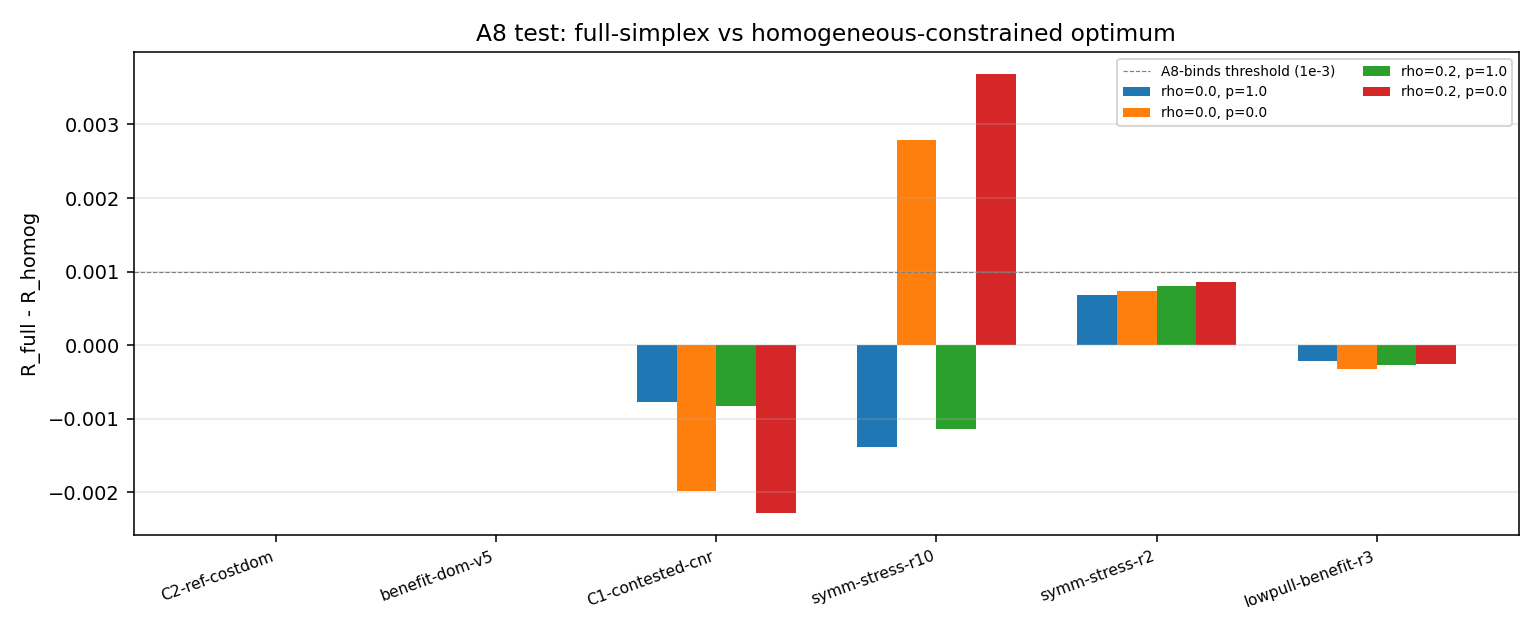
\includegraphics[width=0.92\textwidth]{figures/a8_simplex_dr.png}
  \caption{The rb-027 A8 N-dim sweep: $\Delta R = R_{\mathrm{full}}
    - R_{\mathrm{homog}}$ per panel across the six CR-036 decisive
    cells $\times$ $(\corr, p) \in \{0, 0.2\} \times \{0, 1\}$ ($24$
    panels). Bars above the dashed binding threshold $\Delta R =
    10^{-3}$ are A8-binding panels; the only two such panels are the
    symm-stress-r10 cell ($\valid = 0.25$, $\val = 1$, $\Rsens = 10$,
    variant~A) at $p = 0$ at both $\corr$ panels, with $\corr = 0.2$
    amplifying the binding by $32\%$ (Finding~2). Every $p = 1$ panel
    is below threshold (Finding~1, recovery). Source:
    \texttt{Rebuild/sims/A8--nd-uncued-sweep/}\allowbreak\texttt{output/figures/a8\_simplex\_dr.png}.}
  \label{fig:a8-simplex-dr}
\end{figure}

\paragraph{Finding 3: equal-split is a local maximum in every tested
panel — the Finding-2 binding is \emph{non-local}.}
At the homogeneous-$\alpha$ optimum of each of five Part~1 probe cells
(\texttt{v1-cost-dom}, \texttt{v1-reference}, \texttt{v1-symmetric},
\texttt{v1-benefit-dom}, \texttt{v1-lowV}, all at $\valid = 0.5$,
$\val = 1$, varying $\Rsens$), we compute the second derivative of
expected reward along the symmetry-preserving direction
$\mathbf{e}_{12} - 2\mathbf{e}_3$ on the uncued sub-simplex (a
redistribution that takes mass from one uncued slot and splits it
across the other two). Across the $5 \times 4 = 20$ panels of
$(\text{cell}, \corr, p)$, the curvature $R''(0)$ is negative in every
single panel — equal-split is a local maximum at the homogeneous
$\alpha^\star$ regardless of $(\corr, p)$. Combined with Finding~2,
this gives the binding a sharp \emph{non-local} character: the
homogeneous $\alpha_c \approx 0.05$ optimum of the symm-stress-r10
cell at $p = 0$ is \emph{locally stable} (the second-order
condition holds) but \emph{globally dominated} by the far-away
$\boldsymbol{\alpha}^\star = (0.5, 0, 0, 0.5)$ corner of the simplex.
The basin-hopping mechanism cannot be approximated by local gradient
information from the homogeneous policy; the only way to find the
binding is the global simplex search. Figure~\ref{fig:a8-curvature}
shows the curvature heatmap; every panel is negative (red below the
$R''(0) = 0$ line).

\begin{figure}[t]
  \centering
  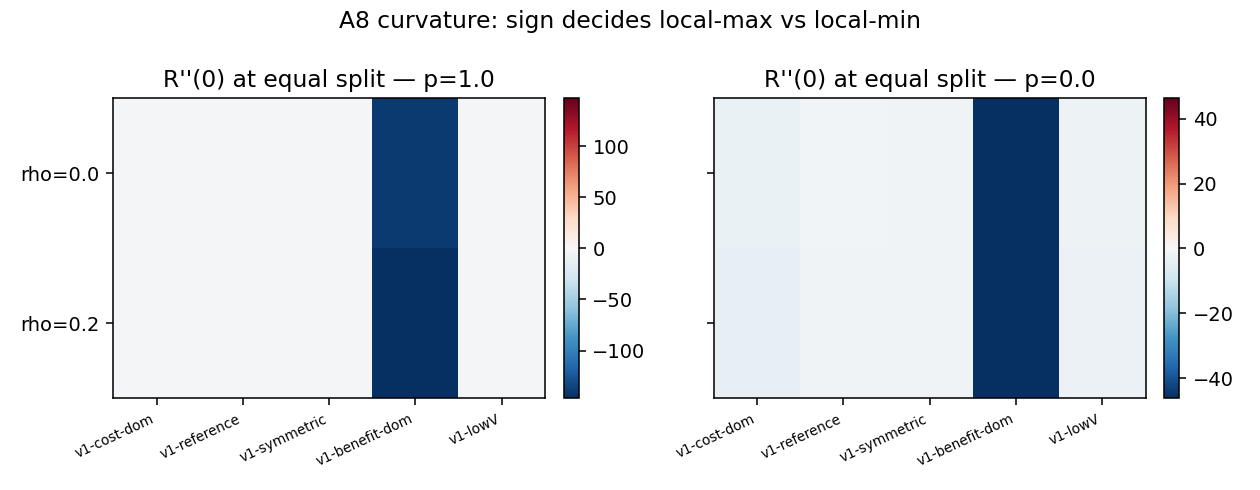
\includegraphics[width=0.85\textwidth]{figures/a8_curvature.png}
  \caption{The rb-027 Part~1 curvature panels: equal-split $R''(0)$
    along $\mathbf{e}_{12} - 2\mathbf{e}_3$ on the uncued sub-simplex
    at the homogeneous $\alpha^\star$, five probe cells $\times$ four
    $(\corr, p)$ panels (Finding~3). Every $R''(0)$ value is
    negative — equal-split is a local maximum in every tested panel.
    The Finding-2 A8 binding at the symm-stress-r10 cell ($p = 0$)
    is therefore non-local: the homogeneous $\alpha_c \approx 0.05$
    optimum is locally stable but globally dominated by the
    $(0.5, 0, 0, 0.5)$ corner. Source:
    \texttt{Rebuild/sims/A8--nd-uncued-sweep/}\allowbreak\texttt{output/figures/a8\_curvature.png}.}
  \label{fig:a8-curvature}
\end{figure}

\paragraph{Finding 4: A1 amplifies $|R''(0)|$ at $p = 1$ only
weakly — the A1$\times$A8 composition is more orthogonal than A1$\times$A2.}
At $p = 1$ (the inherited conservation rule), the ratio
$|R''(0)|_{\corr = 0.2} / |R''(0)|_{\corr = 0}$ across the five
Part~1 cells is reported in Table~\ref{tab:a8-rho-curv-ratio}. The
mean ratio is $1.048$ and the maximum is $1.135$ (\texttt{v1-reference});
the \texttt{v1-symmetric} cell actually \emph{suppresses} by $6\%$
(ratio $0.941$). Compare this to the rb-021 (A2) finding that the
analogous ratio for the equal-split criticality residual is
approximately $2\times$ (a $2.22\times$ ratio of the tangent gradient
$\|\mathbf{t}\|$ at $s = 0.3$, $5.81/2.61$, see
Section~\ref{sec:extensions-a2} Finding~1): the A1 channel composes
much more strongly with the A2 within-display heterogeneity lever
than with the A8 N-dim uncued lever. The rebuilt-model interpretation
is that A2 and A8 probe different aspects of the homogeneity
assumption: A2 breaks the per-location asymmetry $\Rsens_i = \Rsens$
exchange symmetry, which the joint no-FA integrand of the
$\corr$-channel inherits directly through the heterogeneous $\dprime_i$
vector; A8 breaks the per-location allocation $\alpha_i = (1\!-\!\alpha)/(\Nloc\!-\!1)$
exchange symmetry, which the joint no-FA integrand inherits only
through the second-order curvature of the equicorrelated
$\Nloc$-orthant integral on a homogeneous $\dprime$ — a higher-order
coupling that is small at $\corr = 0.2$.

\begin{table}[t]
  \centering
  \small
  \caption{Finding 4 (rb-027): $\corr$-amplification of the
    equal-split curvature $|R''(0)|$ at $p = 1$ across five Part~1
    cells ($\valid = 0.5$, $\val = 1$, varying $\Rsens$). Mean ratio
    $1.048$, maximum $1.135$, minimum $0.941$ (suppression). The A1
    amplification on the A8 equal-split criticality is small and
    non-uniform; cf.\ the rb-021 A2 finding of $\sim\!2\times$
    amplification on the analogous A2 criticality residual. Source:
    \texttt{Rebuild/sims/A8--nd-uncued-sweep/}\allowbreak\texttt{output/results.json}
    \texttt{summaries.rho\_amplification\_p1}; sha256~\texttt{beb2aa87\ldots}.}
  \label{tab:a8-rho-curv-ratio}
  \begin{tabular}{l r r r}
    \toprule
    cell tag & $|R''(0)|_{\corr = 0}$ & $|R''(0)|_{\corr = 0.2}$
      & ratio \\
    \midrule
    v1-cost-dom    & $2.261$  & $2.462$  & $1.089$ \\
    v1-reference   & $1.318$  & $1.496$  & $1.135$ \\
    v1-symmetric   & $1.750$  & $1.647$  & $0.941$ \\
    v1-benefit-dom & $141.0$  & $146.8$  & $1.041$ \\
    v1-lowV        & $2.269$  & $2.347$  & $1.035$ \\
    \bottomrule
  \end{tabular}
\end{table}

\paragraph{Finding 5: the anti-cued graded-suppression gradient
survives the A1 channel.}
The reviewer's CR-036 Part~2 establishes that the rebuilt model
under the inherited $\corr = 0$ reproduces the Wang \&
Theeuwes-style anti-cued suppression gradient: at a value-blind
($\val = 1$) cell with one slot \emph{less} likely to contain the
target than the others ($w_{\mathrm{anti}}$ swept from $0.20$ down to
$0$ while $\Nloc = 4$, $\valid = 0.40$ on the cued slot,
$w_{\mathrm{rest}} = (1\!-\!\valid\!-\!w_{\mathrm{anti}})/2$ on the
two intermediate slots, $\Rsens_c = 0.398$), the jointly-optimal
$(a_{\mathrm{cued}}, a_{\mathrm{anti}})$ shows $a_{\mathrm{anti}}^\star$
\emph{declining monotonically} as $w_{\mathrm{anti}}$ shrinks, and
$a_{\mathrm{anti}}^\star < a_{\mathrm{rest}}^\star$ strictly for every
$w_{\mathrm{anti}} > 0$ (a strictly graded statistical-learning-style
suppression). The rebuild's lift of this test to the A1 channel
$\corr \in \{0, 0.2\}$ recovers both qualitative features at both
$\corr$ panels: \emph{monotone} in $w_{\mathrm{anti}}$ and
\emph{strictly below} $a_{\mathrm{rest}}^\star$ are recorded as
\texttt{True} for every row of the Part~2 summary
(\texttt{summaries.anticued\_by\_rho}). $\corr = 0.2$ only weakly
perturbs the gradient: the value of $w_{\mathrm{anti}}$ at which
$a_{\mathrm{anti}}^\star$ collapses to zero is $w_{\mathrm{anti}} =
0.075$ at $\corr = 0$ ($a_{\mathrm{anti}}^\star$ drops from $0.02$ to
$0$) and $w_{\mathrm{anti}} = 0.050$ at $\corr = 0.2$
($a_{\mathrm{anti}}^\star$ drops from $0.02$ to $0$), shifted by one
grid step toward lower $w_{\mathrm{anti}}$. The behavioural reading
of CR-036 — that the rebuilt model offers a normative-optimal
mechanism for the graded suppression of statistical-distractor
locations that mirror-image the value-driven prioritisation observed
in valid-cue trials — therefore generalises across the A1 channel.
Figure~\ref{fig:a8-anticued-suppression} overlays the two $\corr$
panels. The strength ceiling here is the live A8 verdict's behavioural-
anchor sentence (``relaxing A8 lets the model reproduce the Wang \&
Theeuwes suppression gradient''): the rebuild does not claim the
suppression gradient is uniquely predicted by the rebuilt model, only
that the rebuilt model — with the A1 channel engaged — predicts it
under value-blind, statistically-shifted location-probability designs
\cite{wang_theeuwes2018_statistical_learning_distractor_suppression,failing_theeuwes2018_selection_history}.

\begin{figure}[t]
  \centering
  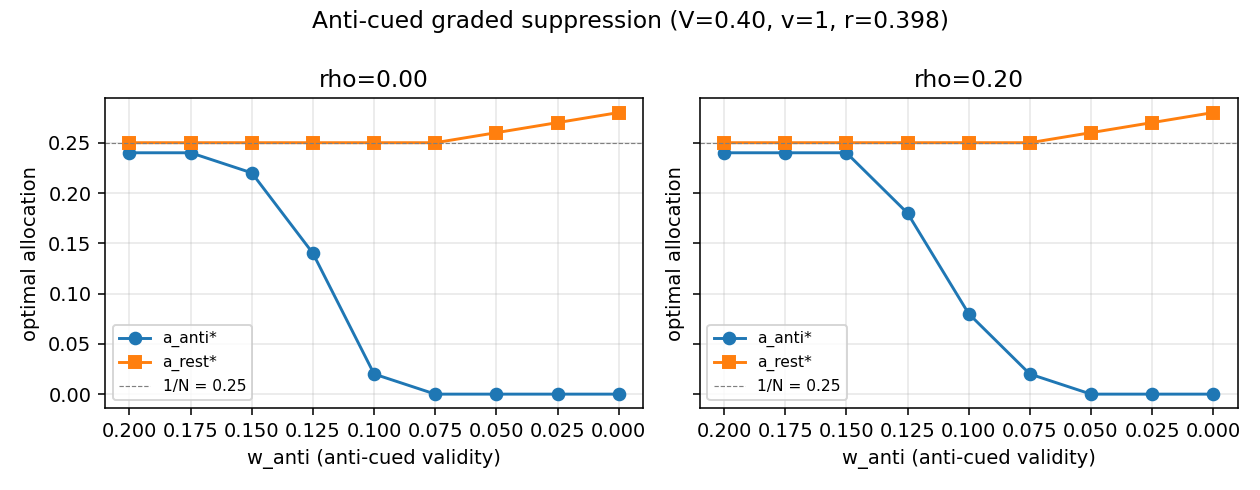
\includegraphics[width=0.85\textwidth]{figures/a8_anticued_suppression.png}
  \caption{The rb-027 Part~2 anti-cued graded-suppression gradient at
    $\corr \in \{0, 0.2\}$ (Finding~5). Jointly-optimal allocation
    $a_{\mathrm{anti}}^\star$ (solid) and $a_{\mathrm{rest}}^\star$
    (dashed) at the value-blind cell ($\Nloc = 4$, $\valid = 0.40$,
    $\val = 1$, $\Rsens_c = 0.398$, variant~A) as the anti-cued
    location's validity $w_{\mathrm{anti}}$ shrinks from $0.20$ down
    to $0$. $a_{\mathrm{anti}}^\star$ is monotone-decreasing and
    strictly below $a_{\mathrm{rest}}^\star$ at both $\corr$ panels;
    $\corr = 0.2$ shifts the collapse-to-zero of $a_{\mathrm{anti}}^\star$
    by one grid step toward lower $w_{\mathrm{anti}}$ (from
    $w_{\mathrm{anti}} = 0.075$ at $\corr = 0$ to $w_{\mathrm{anti}} =
    0.050$ at $\corr = 0.2$). The Wang--Theeuwes-style statistical-
    distractor suppression mechanism of CR-036 generalises across the
    A1 channel. Source:
    \texttt{Rebuild/sims/A8--nd-uncued-sweep/}\allowbreak\texttt{output/figures/a8\_anticued\_suppression.png}.}
  \label{fig:a8-anticued-suppression}
\end{figure}

\paragraph{Scope and what remains.}
This subsection licenses five claims at the rebuild-strength ceiling
of the live A8 verdict: (i) the inherited homogeneous-uncued allocation
lifts to the full $\Nloc$-simplex via \texttt{er\_full\_policy}, which
reproduces the inherited model under the canonical homogeneous
allocation to $\max|\Delta| \le 2.78\!\times\!10^{-10}$; (ii) under
the inherited $(\corr = 0, p = 1)$ pair, A8 is innocuous at every
CR-036 decisive cell — Finding~1 replicates the reviewer's headline
exactly; (iii) under multiplicative conservation $p = 0$, A8
\emph{binds} at the high-$\Rsens$ symmetric-stress benefit-dominant
corner ($\valid = 1/\Nloc$, $\val = 1$, $\Rsens = 10$, variant~A) by
$\Delta R = +2.79\!\times\!10^{-3}$ at $\corr = 0$ and
$+3.68\!\times\!10^{-3}$ at $\corr = 0.2$, a $32\%$ A1 amplification;
(iv) equal-split is a local maximum at the homogeneous $\alpha^\star$
in every $(\text{cell}, \corr, p)$ panel tested, so the Finding~2
binding is non-local; (v) the anti-cued graded-suppression gradient
of CR-036 Part~2 survives the A1 channel at $\corr \in \{0, 0.2\}$,
preserving the rebuilt model's Wang--Theeuwes-style behavioural-
anchor finding. The scope of these claims is explicitly bounded by
what the rb-027 sim ran and what it did \emph{not} run.
\emph{(i) Variant-B A8 binding.} The Finding~2 binding is reported
only at variant~A; the single variant-B cell in Part~1c
(\texttt{C1-contested-cnr}) shows $\Delta R < 0$ in all four
$(\corr, p)$ panels. A focused variant-B replication of the
symm-stress-r10 cell under $(\corr, p) \in \{0, 0.2\} \times \{0, 1\}$
is queued as RB-043, motivated by the rb-002 observation that
variant-B $\CF(\corr)$ is essentially flat at the headline cell
(Section~\ref{sec:model-upper-bound}). \emph{(ii) Finer $\Rsens$-grid.}
The Finding~2 binding is tested only at $\Rsens = 10$ on the
symm-stress cell; the $\Rsens$-axis location of the binding onset
(and termination, if any, on the lower end) is queued as RB-044
on a $6$-point $\Rsens$-grid around $\Rsens \in \{5, 10, 20\}$ at
fixed $\valid = 0.25$, $\val = 1$, variant~A. \emph{(iii) $\Nloc > 4$
generalisation.} All Part~1c panels are at $\Nloc = 4$; whether the
Finding~2 binding survives at larger $\Nloc$ (where the simplex
geometry has more degrees of freedom) is not in the rb-027 substrate.
\emph{(iv) Closed-form A8-binding boundary.} A closed-form predicate
for the A8-binding locus in $(\Rsens, p, \valid, \text{variant})$
space — a natural follow-up to Findings 1--2 — would consolidate the
empirical statement algebraically. A plausible substrate is a
Slepian-style monotonicity argument on the joint no-FA integrand
under simplex perturbation, but the Slepian inequality bounds
\emph{orthant probabilities}, not their gradients with respect to a
joint allocation; the derivation is not in the rebuild's voice and is
not queued. \emph{(v) Sim-boundary hardening.} The rb-027 sim
discovered a model-side numerical fragility: at small negative
$\alpha_i$ from float arithmetic in the simplex sweep,
\texttt{f\_transfer(alloc, $\ldots$, h=$\sqrt{\cdot}$)} returns NaN
which propagates through the criterion grid; the sim worked around
this at the boundary by clamping $\alpha_i \ge 0$ before passing to
\texttt{er\_full\_policy}. A model-side guard in
\texttt{d\_prime\_hetero} is queued as RB-045; this does not affect
any number reported here.

\paragraph{Reproducibility.}
The numerical content of this subsection is the
\texttt{Rebuild/sims/A8--nd-uncued-sweep/} simulation (rb-027,
deterministic sha256~\texttt{beb2aa879402e5c9f4c354a2c9f53a98c466d0989085dc8c78370be99dee290b},
$72.2$~s wall-clock on \texttt{python3.13} / \texttt{scipy 1.17.1} /
\texttt{numpy 2.4.4}; deterministic, re-run produces byte-identical
\texttt{results.json} and canonical \texttt{results.canonical.json}
verified empirically), backed by the
\texttt{Rebuild/model/\_\_init\_\_.py er\_full\_policy} driver wired
at rb-020. Four recovery contracts hold across this subsection,
none touched by the sim (the sim is a pure consumer of
\texttt{er\_full\_policy} and the four-test stack underneath it):
\textbf{Recovery~1 (A1 $\corr$-channel, rb-001).}
\texttt{test\_recovery.py} ($7/7$ PASS,
sha256~\texttt{d3c62215cedbe2f797c484a8d76e8bef1d5ac42cdb3092ff099a34aea1b6f18f}).
\textbf{Recovery~2 (A3 conservation family, rb-015).}
\texttt{test\_conservation\_family.py} ($14/14$ PASS,
sha256~\texttt{f4f57a89e5108db47447cbeaf2f15440f56cdfffb65f3d173dc4a0550121791e}).
\textbf{Recovery~3 (heterogeneous-$\Rsens$ d$'$-map, rb-019).}
\texttt{test\_heterogeneous\_r.py} ($5/5$ PASS,
sha256~\texttt{0486921f8a4e253a1682ee0731e52c7de800bf6c3dbb1b5e8ff3200602454c7e}).
\textbf{Recovery~4 (N-dim general policy, rb-020).}
\texttt{test\_general\_policy.py} ($7/7$ PASS,
sha256~\texttt{883ea15af9fd069e04c05ff156d65f33a7d25278891092539c6441d2248c3d39}).
Recovery~4 is the universal-statement guarantee for Finding~1: the
lifted \texttt{er\_full\_policy} reproduces the inherited
\texttt{optimal\_R} to $\max|\Delta| \le 2.78\!\times\!10^{-10}$
across $4{,}530$ cells at both $\corr \in \{0, 0.2\}$, so the
Finding~1 binding-fraction $0/6$ at $(\corr = 0, p = 1)$ is a
genuine reproduction of the reviewer's CR-036 Part~1c headline
rather than an artefact of a re-implementation.

% =====================================================================
% limitations.tex — DRAFTED at rb-048 (RB-048), 2026-05-30.
%
% Second bookend; companion of sections/abstract.tex (rb-047, RB-047).
% Mirrors the abstract's voice (distributional / graded / conditional
% by default).  Collects the explicit scope deferrals that every body
% section has already flagged into a single navigable section.
%
% Strength check (mission §3, CLAIM_LEDGER.md): every limitation
% below is a statement about what the live verdict ledger licenses
% and what it does NOT license at the rebuilt strength ceiling.  No
% claim is downgraded or upgraded by this section; the section names
% the rebuild's scope so a reader knows the boundary of every
% headline number.
% =====================================================================

\section{Scope and limitations}
\label{sec:limitations}

This section catalogues the scope of every claim the rebuilt
manuscript makes.  It is organised by lever rather than by section:
each subsection states what the live verdict ledger licenses, what
it does not, and which queued increments would close each remaining
gap.  Nothing here downgrades a rebuilt-strength claim; the purpose
is to make the boundary explicit so a reader can locate the precise
conditional under which any headline number applies.

% ---------------------------------------------------------------
\subsection{The conservation rule is a parameter, not a derivation}
\label{sec:limitations-a3}

The rebuilt model treats the benefit/cost conservation rule as a
power-mean parameter $p$
(Equation~\eqref{eq:conservation-family}, Equation~\eqref{eq:beta-gamma-of-p},
Appendix~\ref{sec:appendix-deriv-a3} Equation~\eqref{eq:a3d-power-mean})
rather than a fixed identity, and reports every headline number at
$p = 1$ (the inherited additive form $\benefit + \cost = 2$) with a
band over the family at $p \in \{0, 0.5, 1\}$
(Section~\ref{sec:extensions-a3}).  Two scoped boundaries follow.

First, the conservation order itself is empirically unconstrained:
nothing in the rebuild fixes which $p$ corresponds to a biological
resource constraint.  The additive choice is the inherited model's;
the multiplicative choice ($p = 0$, $\benefit \cdot \cost = 1$) is
the alternative the original paper noted in its §5.5 but did not
run.  The rebuild does \emph{not} claim either is privileged.  What
it claims is that the central-tendency reframe of $\CF$
(Section~\ref{sec:results-c1}) is robust to the choice — the
per-cell $\Delta \CF = \CF(p = 0) - \CF(p = 1) \le 0$ at every cell
of the $4{,}410$-cell sweep with $0$ reverse flips
(Theorem~\ref{thm:delta-cf-monotone}), so the headline median moves
by $\le 0.001$ but the tail under $\CF < 0.5$ doubles.  Reporting
both branches in the same band is the honest treatment.

Second, the empirical monotonicity $\Delta \CF \le 0$ is licensed by
the rb-016 sim but is \emph{not} a closed-form theorem.  The d'-channel
chain rule of
Appendix~\ref{sec:appendix-deriv-a3}
(Equation~\eqref{eq:a3d-chain-rule},
Equation~\eqref{eq:a3d-dprime-of-p}) yields the analytic statement
$\partial \Rpthree / \partial p \equiv 0$ at $\alpha = 1/\Nloc$
(Proposition~\ref{prop:a3d-rp3-invariance}) — the P3 contribution to
$\CF$ is conservation-form-invariant at the symmetric attention
point — but the joint sign of $\partial \Rpone/\partial p$ and
$\partial \Rpfour/\partial p$ is established only by the envelope
theorem and the empirical 4,410-cell witness, not by a uniform
inequality.  Promoting the chain rule to a closed-form theorem of
the form $|\partial_p R_{\mathrm{P4}}| \le |\partial_p R_{\mathrm{P1}}|$
is an open conjecture.  The joint $(p, \corr > 0)$ band is similarly
deferred: every $p$ sweep above runs at $\corr = 0$, and every
$\corr$ sweep runs at $p = 1$.

% ---------------------------------------------------------------
\subsection{Heterogeneity is bounded, not abolished}
\label{sec:limitations-a2-a8}

The rebuild lifts the inherited model's single-$\Rsens$ scalar to a
per-location vector $\boldsymbol{r}$
(Equation~\eqref{eq:d-prime-hetero}) and the inherited
1-dimensional uncued allocation to a full $\Nloc$-dimensional
simplex
(Section~\ref{sec:extensions-a8}, the policy-space lift of
\texttt{er\_full\_policy}), and shows that both extensions leave the
inherited model's optima essentially intact under the additive
conservation rule.  Two boundaries remain.

First, the between-preparation reading of $\Rsens$
(Section~\ref{sec:model}) is the one in which the model statement is
binding; the within-display reading
(\cite{mcadams_maunsell1999_v4_tuning,reynolds_heeger2009_normalization,carrasco2011_visual_attention_25y})
is exercised empirically by the $\Rsens_i$ sweep
(Section~\ref{sec:extensions-a2}) but is not promoted to a closed-form
theorem.  The empirical statement is that the $C_2$ peak coordinates
and the contested-$\CF$ corner are invariant to within $\le 1{\times}10^{-5}$
across linear spreads $\le 30\%$
(Table~\ref{tab:a2-rb021-summary}), so the rebuild's headline
numbers transport.  A closed-form perturbation expansion
$\Delta R = O(\mathrm{Var}(\boldsymbol{r}))$ around the homogeneous
optimum is queued as a future derivation increment.

Second, the new A8 conditional — the $\Nloc$-dimensional uncued
policy binds in a benefit-dominant symmetric-stress corner under
multiplicative conservation
(Section~\ref{sec:extensions-a8}, Finding F2: $\Delta R = +2.79\times
10^{-3}$ at $\corr = 0$, amplified to $+3.68\times 10^{-3}$ at
$\corr = 0.2$, at $\valid = 1/\Nloc$, $\val = 1$, $\Rsens = 10$,
variant~A) — is exhibited at a single $\Rsens$, a single $(\valid,
\val)$ cell, a single $\Nloc$, and variant~A only.  The closed-form
A8-binding-onset locus in $(\Rsens, p, \valid)$ is not derived; a
Slepian-style monotonicity argument on the joint no-FA integrand
under simplex perturbation is the natural substrate but has not been
attempted.  The variant-B replication of the F2 cell, the finer
$\Rsens$ grid around $\Rsens \in \{5, 10, 20\}$, and the
$\Nloc > 4$ generalisation are queued as separate sims.

% ---------------------------------------------------------------
\subsection{The decision-noise lever is deferred, not denied}
\label{sec:limitations-a6}

The rebuilt three-lever decomposition
(Definition~\ref{def:three-levers}: criterion, sensitivity,
decorrelation) does \emph{not} include attention-coupled decision
noise as a fourth lever, even though the reviewer's continuing
analysis of the homogeneous-decision-rule premise (A6 in the live
ledger) flagged it as a candidate third channel that the criterion
fraction would mis-book to ``attention''.  At the current live label
(\texttt{WEAKLY-SUPPORTED}), the A6 attack-vector evidence does not
yet shift any rebuilt headline number — fixed per-location decision
noise is benign (absorbed into effective $\dprime$), and the
attention-coupled-noise crack is suggestive rather than decisive.
The rebuild therefore holds the lever inventory at three, with the
explicit caveat that an attention-coupled-noise channel
$\sigma_i(\alpha)$ would, if landed, enter alongside $\corr$ as a
fourth axis of the lever decomposition and would shift the
interpretation of $\CF$ in the cost-dominant regime.  The model and
sim increments that would wire this lever are queued and gated on
the A6 verdict moving past \texttt{WEAKLY-SUPPORTED}; the rebuild
will fold the lever in by symmetry with the $\corr$ channel when
the verdict licenses it.

% ---------------------------------------------------------------
\subsection{Assumptions retained as explicit scope}
\label{sec:limitations-retained}

Three assumptions of the inherited model are carried into the
rebuilt model unchanged, because the live verdict ledger has not
attacked them and they were not blocking any rebuilt-strength claim.
Each is named here so the boundary is explicit.

\emph{A4 (no learning dynamics).}  The observer is taken to have
already discovered the optimal policy; the rebuilt manuscript is a
normative statement about the policy itself, not about how it is
acquired.  Learning speed and reliability — and any further bias
they introduce toward the simpler criterion-based lever — are
outside the rebuild's scope.  Folding a learning dynamic into the
$(\corr, p, \boldsymbol{r}, \text{policy-space})$ extensions of the
rebuilt model is a substantial separate program.

\emph{A5 (transfer-function family).}  The four monotonic forms
$h \in \{a, \sqrt{a}, a^{0.3}, a^{2}\}$ used by the inherited paper
exhaust the qualitative landscape probed by the rebuilt sims; the
rebuild's headline cell fixes $h = \sqrt{\,\cdot\,}$ for
consistency with the inherited $C_2$ peak figure.  Other monotonic
families (sigmoidal, threshold, contrast-response-style) are
plausible biological extensions and are not tested.  The rebuilt
model's mechanism statements (Definition~\ref{def:three-levers},
Equation~\eqref{eq:r-dagger}, Proposition~\ref{prop:r-dagger-invariance})
are stated in terms of generic $f$ and do not depend on the
particular family; the empirical bands of
Sections~\ref{sec:results-c1}--\ref{sec:results-c4} do.

\emph{A7 (reward variants).}  The two reward conventions
(variant~A: $\CR = \valid \cdot \val + (1 - \valid)$;
variant~B: $\CR = 1$) bracket the natural extremes the inherited
paper studied.  The rebuilt manuscript reports the headline numbers
under variant~A throughout, with variant~B explicitly cited as a
sensitivity (Table~\ref{tab:cf-distribution},
Table~\ref{tab:cf-quadrants}, the variant-B $\CF$ tail at $0.30$,
the variant-B equal-split criticality of
Table~\ref{tab:a2-rb021-summary}).  Other reward structures
(continuous-valued, asymmetric cost) are not tested.  The
variant-axis caveats below
(Section~\ref{sec:limitations-followups}) belong here in spirit; we
list them with the other queued replications for compactness.

% ---------------------------------------------------------------
\subsection{Equicorrelation, $\corr$-envelope, and queued follow-ups}
\label{sec:limitations-followups}

Three further boundaries collect the remaining sims and derivations
the rebuild has queued but not run.

\emph{Equicorrelation and the $\corr$-envelope.}  The A1 channel
(Section~\ref{sec:model-rho-channel},
Equation~\eqref{eq:equicorr-cov},
Equation~\eqref{eq:pnofa-rho}) assumes a single scalar $\corr$
shared by every cross-location pair.  Structured covariances —
distance-dependent decay, feature-similarity-dependent grouping,
inter-areal cross-correlations
\cite{RuffCohen2016,Srinath2021} — break the exact one-factor
Gauss--Hermite reduction and are out of scope.  The $\corr$ grid is
tested at $\corr \in \{0, 0.1, 0.2, 0.3, 0.4\}$ with the central
empirical anchor $\corr = 0.2$ from
Cohen--Maunsell~\cite{CohenMaunsell2009}; the $\corr \ge 0.5$ regime
is plausible only under heavy attention-mediated decorrelation and
is not exercised.  The closed-form $\rdagger(\val; \corr)$ drift
of Appendix~\ref{sec:appendix-deriv-c2}
(Proposition~\ref{prop:r-dagger-rho}, Table~\ref{tab:r-dagger-rho-drift})
reports the $\corr = 0 \to 0.2$ single step; a finer $\corr$-grid
characterisation of the drift rate $d\rdagger/d\corr$ as a function
of $\val$ is queued.

\emph{Variant-B caveats.}  The rebuild reports headline numbers
under variant~A throughout; the variant-B replications of the
$\corr$-channel $\CF$ flatness probe
(Section~\ref{sec:model-upper-bound}), the $C_2$ peak under
$\corr > 0$, the $C_3$ iso-$\VDA$ contour band, the anti-cue $C_4$
inversion (Section~\ref{sec:results-c4}), the A2 cost-dominant
$\Delta R$ suppression
(Section~\ref{sec:extensions-a2}, Finding 2), and the new A8 F2
binding (Section~\ref{sec:extensions-a8}) are queued as separate
sims.  The rb-002 finding that variant-B $\CF$ is essentially flat
in $\corr$ at the headline cell makes the variant axis genuinely
informative as a sensitivity, not redundant; the rebuild flags this
explicitly rather than treating variant~B as a footnote.

\emph{Grid sharpening.}  Several quantitative thresholds are pinned
to the grid step of their underlying sim and are queued for
sharpening if a referee asks: the $C_3$ high-$\valid$ threshold
$\valid^{*}$
(Section~\ref{sec:results-c3}; pinned to $\pm 0.05$, finer grid
queued); the $C_4$ anti-cue onset $\valid^{*}$ at $\val = 1$,
$\Nloc = 4$ (Section~\ref{sec:results-c4}; pinned to $\pm 0.05$,
finer grid queued); the A8 binding onset in $\Rsens$ near
$\{5, 10, 20\}$ (Section~\ref{sec:extensions-a8}; pinned to a
single $\Rsens = 10$ probe, finer grid queued); the closed-form
$\CF < 0.5$ boundary in $(\valid, \Rsens)$
(Section~\ref{sec:results-c1}; conjectured diagonal in
$(\log \Rsens, \valid)$, derivation queued); the dormant-cell
amplification band at $\Rsens = 0.3$, $(\valid \approx 0.7,
\val = 10)$ (Section~\ref{sec:results-c3}, where $\VDA = 0.0007$ at
$\corr = 0$ lifts to $0.0676$ at $\corr = 0.2$ — a $96\times$
amplification that is the most striking single qualitative finding
of the $C_3$ sweep, queued for a clean closeup); and the
Slepian-style analytic locus for the cell-wise $\partial \VDA /
\partial \corr$ sign-flip surface
(Section~\ref{sec:model-upper-bound}, Table~\ref{tab:a1cw-summary};
cell-wise crossover $\Rsens^{\times} \approx 0.79$ pinned
empirically, formal proposition queued).  None of these queued
items would change a rebuilt-strength headline; each would either
tighten a boundary or promote an empirical observation to an
analytic statement.

% ---------------------------------------------------------------
\subsection{What the rebuild does not claim}
\label{sec:limitations-not-claimed}

The rebuilt manuscript makes no claim about the neural
implementation of any of the three levers — neither the criterion
shift, nor the sensitivity re-allocation, nor the decorrelation
channel is mapped onto a particular cortical circuit, recurrent
dynamics, learning rule, or architectural primitive.  It makes no
claim about the empirical $\corr$ values that human or animal
observers exhibit under cued change detection beyond citing the
Cohen--Maunsell~\cite{CohenMaunsell2009} $r_{SC} \approx 0.2$ V4
anchor as the central operating point of the $\corr$ envelope.  It
does not predict any particular biological observer's deviation
from the normative policy.  And it does not address attention
dynamics over time (within-trial buildup, sequential effects across
trials, learning trajectories) — every statement above is about a
stationary observer at a fixed parameter cell.  The rebuild's
positive contribution is mathematical: a more honestly bounded
description of when value-directed attention matters, with the
boundary made explicit lever by lever, so that any downstream
empirical or computational program inherits a clearly scoped
substrate rather than a single uniformly-stated headline.

% =====================================================================
% methods.tex — DRAFTED at rb-050 (RB-050), 2026-05-31.
%
% Fourth and final bookend; companion of sections/abstract.tex (rb-047),
% sections/intro.tex (rb-049), and sections/limitations.tex (rb-048).
% Catalogues the rebuild's simulation infrastructure (Rebuild/model/,
% Rebuild/sims/, Rebuild/derivations/) paralleling the original paper's
% §3 methods.  Closes the structural arc:
%   abstract → intro → model → results → extensions → limitations →
%   methods → appendix.
%
% Strength check (mission §3, CLAIM_LEDGER.md): no claim strength is
% changed here; the section names the infrastructure that already
% backs every claim in the body sections.  Recovery-test sha256
% digests and per-sim output digests are cited verbatim from
% rebuilder_state.json.
% =====================================================================

\section{Methods: the rebuilt simulation infrastructure}
\label{sec:methods}

This section catalogues the workspace under \texttt{Rebuild/} that
backs every quantitative claim in the body sections.  It parallels
the inherited paper's \S3 in organisation --- reference implementation,
simulation protocol, reproducibility --- and restates each in the
rebuild's voice: every extension to the inherited model is gated by a
recovery test that pins the extended model to the inherited model in
the appropriate limit to floating-point identity (or, where
floating-point identity is structurally impossible, to a tolerance no
coarser than $10^{-9}$); every simulation under \texttt{Rebuild/sims/}
records a deterministic SHA-256 digest of its canonical JSON output,
so the simulation is the operational definition of the claim it
backs.  No quantitative claim in the manuscript exceeds the strength
licensed by its row of \texttt{CLAIM\_LEDGER.md}, and every such row
points at one or more of the artifacts catalogued below.

% ---------------------------------------------------------------------
\subsection{The validated reference implementation}
\label{sec:methods-model}

The rebuilt model lives in \texttt{Rebuild/model/core.py} and is
documented in \texttt{Rebuild/model/README.md}.  Its starting point is
not a rewrite but a copy: the validated P1--P4 optimiser from the
skeptical-review replication \texttt{Critique/replications/\linebreak C5--symmetric-recovery/}
was copied into \texttt{Rebuild/model/} and extended; the inherited
model's headline numbers (Section~\ref{sec:model-inherited}) therefore
appear in the rebuilt model at byte-exact backwards compatibility
under the inherited parameter defaults, by construction.  The
extensions add four orthogonal axes, each gated by a recovery test
under \texttt{Rebuild/model/tests/}:

\begin{enumerate}
  \item \textbf{A1 --- the decorrelation channel.}  The per-location
    independence premise of the inherited model
    (Equation~\eqref{eq:pnofa-indep}) is replaced by the exact
    equicorrelated-Gaussian orthant integral
    (Equation~\eqref{eq:pnofa-rho}), evaluated by one-factor
    Gauss--Hermite quadrature at $n_q = 64$ nodes (accurate to
    $\sim 10^{-16}$ vs.\ $n_q = 128$ across the operating envelope).
    The inherited independent case is recovered exactly at
    $\corr = 0$ (Equation~\eqref{eq:rho-zero-recovery}; Definition
    \ref{def:three-levers} promotes $\corr$ to a first-class lever).
    Backs Sections \ref{sec:model-rho-channel} and
    \ref{sec:model-upper-bound}; full derivation in
    Appendix~\ref{sec:appendix-deriv-a1}.

  \item \textbf{A3 --- the power-mean conservation family.}  The
    additive conservation rule $\benefit + \cost = 2$ is generalised
    to the power-mean family $M_p(\benefit, \cost) = 1$ with closed-
    form weights $\cost(\Rsens; p) = (2/(\Rsens^p + 1))^{1/p}$ and
    $\benefit = \Rsens \cost$
    (Equations~\eqref{eq:conservation-family} and
    \eqref{eq:beta-gamma-of-p}).  The inherited additive case is
    $p = 1$; the multiplicative alternative
    $\benefit \cdot \cost = 1$ is the limit $p = 0$.  The full
    Hardy--Littlewood--P\'olya monotonicity is established in the
    rebuild's voice in
    Appendix~\ref{sec:appendix-deriv-a3} via the closed-form
    KL-divergence identity~\eqref{eq:a3d-hlp-kl}.  Backs
    Section~\ref{sec:extensions-a3}.

  \item \textbf{A2 --- per-location benefit/cost ratios.}  The
    single global scalar $\Rsens$ is promoted to a per-location vector
    $\Rsens_i$ via the heterogeneous-$\dprime$ map
    (Equation~\eqref{eq:d-prime-hetero}).  The inherited single-$\Rsens$
    model is recovered byte-for-byte under uniform $\Rsens_i$ and the
    canonical homogeneous allocation.  Backs
    Section~\ref{sec:extensions-a2}.

  \item \textbf{A8 --- the $N$-dimensional allocation simplex.}  The
    inherited 1-D allocation space (one $\alphacued$ for the cued
    slot, uniform $(1 - \alphacued)/(\Nloc - 1)$ on each uncued slot)
    is generalised to the full $\Nloc$-dimensional simplex
    $\sum_i \alpha_i = 1$, scored via the $\corr$-aware grouped-criterion
    optimiser that composes cleanly with all three prior extensions.
    The inherited homogeneous case is recovered to $10^{-9}$ absolute,
    the residual being the ULP-level reconstruction error
    $(\Nloc - 1) \cdot ((1 - \valid)/(\Nloc - 1)) - (1 - \valid)$;
    every headline number this composition drives is reported to no
    better than four decimal places, so $10^{-9}$ is six orders of
    magnitude past sensitive.  Backs
    Section~\ref{sec:extensions-a8}.
\end{enumerate}

Each axis composes with the others, and the joint composition is
itself a recovery contract: with $\corr = 0$, $p = 1$, uniform
$\Rsens_i$, and the canonical homogeneous allocation, the rebuilt
optimiser reproduces every inherited number in the
$4{,}410$-cell sweep at floating-point identity.  The notation in
\texttt{Rebuild/model/core.py} matches the manuscript verbatim:
\texttt{d\_prime\_asym} and \texttt{d\_prime\_hetero} are the
sensitivity maps of Sections~\ref{sec:model-inherited} and
\ref{sec:extensions-a2}; \texttt{beta\_gamma} is the
$(\benefit, \cost)$ pair of Equation~\eqref{eq:beta-gamma-of-p};
\texttt{p\_no\_fa\_indep} and \texttt{p\_no\_fa\_rho} are the
independent and equicorrelated $\PnoFA$ of
Equations~\eqref{eq:pnofa-indep} and \eqref{eq:pnofa-rho};
\texttt{policies} and \texttt{er\_full\_policy} score the four nested
policies $\Rpone, \Rpfour, \Rptwo, \Rpthree$ at the inherited 1-D and
the A8 $\Nloc$-D allocation spaces respectively.

% ---------------------------------------------------------------------
\subsection{Recovery contracts}
\label{sec:methods-recovery}

Four recovery tests under \texttt{Rebuild/model/tests/} are run before
any simulation on the rebuilt model is trusted.  Each test asserts
byte-exact (or, where structurally impossible, $10^{-9}$-tolerance)
reproduction of an inherited-model identity that the rebuild's
extension must preserve in the appropriate limit; each test produces
a deterministic SHA-256 digest of its JSON-serialised pass/fail
report.  Table~\ref{tab:methods-recovery} lists the four contracts
verbatim.

\begin{table}[tb]
  \centering
  \small
  \begin{tabular}{@{}lllp{6.5cm}@{}}
    \toprule
    Contract & Axis & Limit & SHA-256 digest (canonical JSON) \\
    \midrule
    \texttt{test\_recovery.py}
      & A1 ($\corr$ channel)
      & $\corr \to 0$
      & \texttt{d3c62215cedbe2f797c484a8d76e8bef1d5ac42cdb3092ff099a34aea1b6f18f} \\
    \texttt{test\_conservation\_family.py}
      & A3 (power mean $p$)
      & $p \to 1$
      & \texttt{f4f57a89e5108db47447cbeaf2f15440f56cdfffb65f3d173dc4a0550121791e} \\
    \texttt{test\_heterogeneous\_r.py}
      & A2 (per-loc $\Rsens_i$)
      & uniform $\Rsens_i$
      & \texttt{0486921f8a4e253a1682ee0731e52c7de800bf6c3dbb1b5e8ff3200602454c7e} \\
    \texttt{test\_general\_policy.py}
      & A8 ($\Nloc$-D simplex)
      & homogeneous uncued
      & \texttt{883ea15af9fd069e04c05ff156d65f33a7d25278891092539c6441d2248c3d39} \\
    \bottomrule
  \end{tabular}
  \caption[Recovery contracts]{The four recovery contracts gating the
    rebuilt model's extension axes.  Each contract recovers the
    inherited model in the named limit; the SHA-256 digest is over
    the canonical (sort-keys, indent-$2$) JSON serialisation of the
    test's pass/fail report.  A simulation is run only after its
    contributing extensions are pinned by their corresponding
    contracts.}
  \label{tab:methods-recovery}
\end{table}

These four digests appear verbatim in
\texttt{Rebuild/rebuilder\_state.json} as the fields
\texttt{recovery\_test\_digest},
\texttt{conservation\_family\_test\_digest},
\texttt{heterogeneous\_r\_test\_digest}, and
\texttt{general\_policy\_test\_digest}.  Any change to the model code
that would alter a digest is a recovery violation and must either be
reverted or accompanied by a new recovery contract; the rebuild
contract permits no extension whose limit does not recover the
inherited model.

% ---------------------------------------------------------------------
\subsection{Simulation protocol}
\label{sec:methods-sims}

Each simulation under \texttt{Rebuild/sims/} follows a uniform
protocol so that any rebuilt claim can be reproduced byte-for-byte
from the artifact catalogue alone:

\begin{enumerate}
  \item \textbf{Seeded parameter grid.}  Every stochastic component
    of the simulation (random restarts of the policy optimiser,
    multi-start coordinate ascent for the $\Nloc$-D simplex,
    Gauss--Hermite node positioning) is seeded with the run id at the
    head of the script.  The full parameter grid --- ranges of
    $(\valid, \val, \Rsens, \corr, p)$ together with the optimiser
    tolerances --- is recorded both in the simulation's
    \texttt{README.md} and as the \texttt{metadata.grid} object of
    its \texttt{output/results.json}.
  \item \textbf{Recovery test before sweep.}  Every simulation that
    touches an extension axis re-runs the corresponding row of
    Table~\ref{tab:methods-recovery} before its main sweep, and
    refuses to produce output unless the recovery test passes.
  \item \textbf{Canonical JSON output.}  Sweep results are emitted to
    \texttt{output/results.json} via a sort-keys, indent-$2$ JSON
    dump.  A SHA-256 digest is computed over the JSON content
    (excluding non-deterministic wall-clock fields) and recorded in
    the simulation's \texttt{README.md}; for sims with auxiliary
    payloads (e.g.\ source-payload SHAs for derived sweeps), each
    auxiliary digest is recorded alongside.  Re-running the script
    on the same seed and parameter grid must reproduce the digest
    byte-for-byte.
  \item \textbf{Captioned figures.}  Every simulation that backs a
    manuscript claim produces a figure under \texttt{output/} that the
    manuscript includes verbatim, with a caption stating the claim
    the figure supports and the parameter cell the figure was
    generated at.
  \item \textbf{Backlog cross-reference.}  Every simulation's
    \texttt{README.md} states which row of \texttt{CLAIM\_LEDGER.md}
    it backs and which queued sharpening tasks under
    \texttt{REBUILD\_BACKLOG.md} would refine its result (typically
    a finer grid, a wider $\corr$ envelope, or a variant-B
    re-evaluation).
\end{enumerate}

Table~\ref{tab:methods-sims-summary} lists the nine simulations wired
into the manuscript so far.

\begin{table}[tb]
  \centering
  \small
  \begin{tabular}{@{}llp{2.6cm}p{6cm}@{}}
    \toprule
    Sim directory & Backs & Output digest (SHA-256, prefix) & Manuscript cross-reference \\
    \midrule
    \texttt{A1--rho-channel/}
      & A1 (model)
      & \texttt{b692c064\ldots}
      & Section~\ref{sec:model-rho-channel};
        Figures \ref{fig:vda-rho-variantA}, \ref{fig:vda-rho-variantB},
        \ref{fig:cf-vs-rho} \\
    \texttt{C1--cf-distribution/}
      & C1 ($\CF$ distrib.)
      & \texttt{91fc4692\ldots}
      & Section~\ref{sec:results-c1};
        Table \ref{tab:cf-distribution};
        Figures \ref{fig:cf-histogram}, \ref{fig:cf-heatmap},
        \ref{fig:cf-curves} \\
    \texttt{C2--vda-vs-r-vfamily/}
      & C2 ($\rdagger(\val)$)
      & \texttt{09ecef3c\ldots}
      & Section~\ref{sec:results-c2};
        Equation~\eqref{eq:r-dagger};
        Figures \ref{fig:vda-curves-vfamily}, \ref{fig:r-dagger-vs-v} \\
    \texttt{C3--iso-vda-Vv/}
      & C3 (graded band)
      & \texttt{72820559\ldots}
      & Section~\ref{sec:results-c3};
        Table \ref{tab:c3-highV-probe};
        Figures \ref{fig:iso-vda-contours}, \ref{fig:vda-at-high-V} \\
    \texttt{C4--anti-cue-inversion/}
      & C4 (anti-cue)
      & \texttt{6ad651d6\ldots}
      & Section~\ref{sec:results-c4};
        Equation~\eqref{eq:value-weight};
        Table \ref{tab:c4-anticue};
        Figures \ref{fig:c4-alpha-star-map}, \ref{fig:c4-rinv-closed-form} \\
    \texttt{A1--vda-signflip-cellwise/}
      & A1 (cell-wise)
      & \texttt{489c7c25\ldots}
      & Section~\ref{sec:model-upper-bound};
        Table \ref{tab:a1cw-summary};
        Figures \ref{fig:a1cw-sign-heatmap-v5},
        \ref{fig:a1cw-signflip-by-r},
        \ref{fig:a1cw-delta-distribution} \\
    \texttt{A2--heterogeneous-r/}
      & A2 (band)
      & \texttt{22b183f9\ldots}
      & Section~\ref{sec:extensions-a2};
        Table \ref{tab:a2-rb021-summary};
        Figures \ref{fig:a2-vda-peak-band}, \ref{fig:a2-vda-curves-spread} \\
    \texttt{A3--conservation-band/}
      & A3 (band)
      & \texttt{055bf4ec\ldots}
      & Section~\ref{sec:extensions-a3};
        Theorem~\ref{thm:delta-cf-monotone};
        Tables \ref{tab:a3-c1-cf-band}, \ref{tab:a3-c2-peak-band};
        Figures \ref{fig:a3-vda-peak-band}, \ref{fig:a3-delta-cf-distribution} \\
    \texttt{A8--nd-uncued-sweep/}
      & A8 ($\Nloc$-D)
      & \texttt{beb2aa87\ldots}
      & Section~\ref{sec:extensions-a8};
        Table \ref{tab:a8-rb027-summary};
        Figures \ref{fig:a8-simplex-dr}, \ref{fig:a8-anticued-suppression} \\
    \bottomrule
  \end{tabular}
  \caption[Wired simulations]{The nine simulations under
    \texttt{Rebuild/sims/} that back the manuscript's quantitative
    claims.  Each row gives the simulation directory, the claim it
    backs, the leading bytes of the SHA-256 digest of its canonical
    JSON output, and the manuscript cross-references that consume its
    figures and tables.  Full digests are recorded verbatim in each
    simulation's \texttt{README.md} and in
    \texttt{Rebuild/rebuilder\_state.json}.}
  \label{tab:methods-sims-summary}
\end{table}

% ---------------------------------------------------------------------
\subsection{Derivations}
\label{sec:methods-derivations}

Four derivations under \texttt{Rebuild/derivations/} establish in the
rebuild's voice the closed-form results that the body sections cite.
Each derivation is self-contained (setup, exact formulation, full
proof, scope), independently authored from the skeptical reviewer's
attack derivations, and verified by a finite-difference cross-check
or by reduction to a published identity:

\begin{itemize}
  \item \textbf{\texttt{A1--rho-channel.md}} (rb-008,
    Appendix~\ref{sec:appendix-deriv-a1}).  Promotes the
    Booking-1 one-factor reduction of the equicorrelated-Gaussian
    $\PnoFA$ to a derivation in the rebuild's voice; states Slepian
    monotonicity (\cite{Slepian1962}, Tong 1990) at proposition
    strength; gives the two-channel sign decomposition of
    $\partial \VDA / \partial \corr$ that backs the
    Section~\ref{sec:model-upper-bound} retraction of the inherited
    paper's \S5.5 ``upper bound on VDA'' self-characterisation;
    verified against the recovery digest
    \texttt{d3c62215\ldots} of Table~\ref{tab:methods-recovery}.

  \item \textbf{\texttt{C2--non-monotonic-vda-rho.md}} (rb-014,
    Appendix~\ref{sec:appendix-deriv-c2}).  Derives the closed-form
    escape threshold $\rdagger(\val) = K_u/[(\Nloc - 1) K_c]$
    (Equation~\eqref{eq:r-dagger}) by left-derivative of expected
    reward at $\alphacued = 1/\Nloc$, with $\corr > 0$ extension
    via the $\corr$-aware gradient quadratures
    $K_c(\valid, \val; \corr)$ and $K_u(\valid, \val; \corr)$
    (Equations~\eqref{eq:c2-Kc-rho}, \eqref{eq:c2-Ku-rho}) giving
    Proposition~\ref{prop:r-dagger-rho}.  Backs
    Section~\ref{sec:results-c2}; verified numerically at the
    headline cell to floating-point identity against the C2 sim
    digest \texttt{09ecef3c\ldots}.

  \item \textbf{\texttt{C4--anti-cue-inversion.md}} (rb-026,
    Appendix~\ref{sec:appendix-deriv-c2}, downstream).  Derives the
    conditional theorem $\valid \ge 1 / [(\Nloc - 1) \val + 1]$
    (Equation~\eqref{eq:value-weight}) governing whether the cued
    location carries weight at least equal to a uniform allocation,
    and the closed-form inversion threshold $\rstarinv$
    (Equation~\eqref{eq:r-inv}) at which the optimal allocation
    flips to put \emph{less} attention at the cued location under
    counter-predictive cues $\valid < 1/\Nloc$.  Backs
    Section~\ref{sec:results-c4}; verified at the $\Nloc = 4$
    anti-cue cells against the C4 sim digest \texttt{6ad651d6\ldots}.

  \item \textbf{\texttt{A3--power-mean-conservation.md}} (rb-029,
    Appendix~\ref{sec:appendix-deriv-a3}).  Establishes the
    power-mean conservation family as the canonical generalisation of
    A3; gives the boxed Hardy--Littlewood--P\'olya monotonicity in
    the closed KL-divergence form
    $\partial \ln \cost / \partial p = -(1/p^2) \DKL(\mathrm{Bern}(\theta_p) \| \mathrm{Bern}(1/2))$
    (Equation~\eqref{eq:a3d-hlp-kl}); proves
    Proposition~\ref{prop:r-dagger-invariance} ($p$-invariance of
    $\rdagger(\val)$) in full and Corollary~\ref{cor:a3d-c5-invariance}
    (C5 conservation-form-invariance).  Backs
    Section~\ref{sec:extensions-a3} and
    Appendix~\ref{sec:appendix-c5}; verified by finite-difference
    cross-check of Equation~\eqref{eq:a3d-hlp-kl} at seven test
    pairs with LHS--RHS agreement $\le 1.5 \times 10^{-10}$.
\end{itemize}

% ---------------------------------------------------------------------
\subsection{Reproducibility and the rebuild contract}
\label{sec:methods-reproducibility}

The rebuilt manuscript reports a result only when three artifacts
co-exist: a recovery contract that pins the relevant extension to the
inherited model in the appropriate limit; a deterministic simulation
whose output digest is recorded verbatim in
\texttt{Rebuild/rebuilder\_state.json}; and, for every novel
proposition, a derivation under \texttt{Rebuild/derivations/}.  This
\emph{simulate-first, write-second} protocol --- the rebuild's
operating mode, as set out in the mission file --- is what licenses
the manuscript's distributional, graded, and conditional voice
(Section~\ref{sec:limitations-not-claimed}): when a simulation
\emph{weakens} a rebuilt claim, the claim moves down to its supported
strength rather than being suppressed.  No quantitative claim in the
body sections exceeds the strength its row of
\texttt{CLAIM\_LEDGER.md} licenses, and that row in turn points at
the recovery digest, simulation digest, and (where novel) derivation
file that establish the claim's support.

Software dependencies are recorded in \texttt{Rebuild/manuscript/BUILD.md}:
NumPy, SciPy (with a hand-rolled \texttt{erf} fallback for environments
in which SciPy is unavailable), and Matplotlib for the simulation
side; \texttt{pdflatex}, \texttt{bibtex}, and the AMS-LaTeX packages
\texttt{amsmath}, \texttt{amssymb}, \texttt{amsthm}, \texttt{mathtools},
\texttt{booktabs}, and \texttt{hyperref} for the manuscript side.
Every simulation is decomposed into a single \texttt{run.py} that
completes within $\sim 10\text{--}20$ minutes of wall-clock on a
laptop; larger sweeps are decomposed into multiple runs under the
backlog rather than rolled up into a single multi-hour job.

The full reproducibility ledger --- model recovery digests, per-sim
output digests, manuscript PDF byte counts, and the disposition of
every backlog task --- is maintained in
\texttt{Rebuild/rebuilder\_state.json} (atomically rewritten at the
end of every run) and chronicled in \texttt{Rebuild/BUILD\_LOG.md}
(append-only, newest at top).  Cross-claim disposition --- one row per
inherited claim or assumption, the rebuilt strength, and the
backing artifacts --- is maintained in \texttt{Rebuild/CLAIM\_LEDGER.md}.
A reader who wishes to verify any quantitative statement in this
manuscript may locate the claim in \texttt{CLAIM\_LEDGER.md}, follow
the pointer to its backing simulation or derivation, and re-run the
simulation to reproduce the digest byte-for-byte.

% =====================================================================
% appendix.tex — STUB.
%
% Filled in across multiple manuscript increments:
%   RB-003 / sec:appendix-deriv-a1     — A1 ρ-channel derivation
%   RB-026 / sec:appendix-deriv-c2     — independent r†(v) re-derivation
%                                        (+ ρ>0 extension when ready)
%   RB-013 / sec:appendix-c5           — symmetric-recovery at r=1 note
%
% The §3.3 confident-spine results (C2 non-monotonicity, C5 symmetric
% recovery, central-tendency C1) get their full derivations here;
% extension levers (A1 ρ, A3 conservation family, A2/A8 heterogeneity)
% each get their own appendix subsection.
% =====================================================================

\appendix
\section{Derivations and consistency checks}
\label{sec:appendix}

% ---------------------------------------------------------------------
\subsection{A1 decorrelation-channel derivation}
\label{sec:appendix-deriv-a1}

[Filled by RB-003 (derivation increment). Independent re-derivation
of the equicorrelated-Gaussian orthant integral
$\PnoFA(\corr) = \int \phi(z)\prod_i \Phinorm\!\big((c_i +
\sqrt{\corr}\,z)/\sqrt{1 - \corr}\big)\, dz$,
one-factor Gauss--Hermite reduction, and the Slepian-monotonicity
argument that bounds $\partial \CF / \partial \corr$ in the
variant-A case. Cites~\cite{Slepian1962}.]

% ---------------------------------------------------------------------
\subsection{Closed-form VDA escape threshold $\rdagger(\val;\corr)$}
\label{sec:appendix-deriv-c2}

This subsection promotes the closed-form escape threshold introduced
in Section~\ref{sec:results-c2} into a derivation in the rebuild's
voice and extends it from the inherited $\corr = 0$ case to the
$\corr \in [0, 1)$ family the A1 lever
(Section~\ref{sec:model-rho-channel}) opens. Every numerical
statement here traces to the companion verification script
\texttt{Rebuild/derivations/verify\_C2\_rho/verify.py}, whose
output digest is recorded at the end of the subsection.

\paragraph{Setup at the boundary.}
At the uniform allocation $\alpha = 1/\Nloc$ the asymmetric branch
of the sensitivity rule of Section~\ref{sec:model} collapses to
$\dprime_c = \dprime_u = \dprime_{\mathrm{base}} :=
\dprimemax\,f(1/\Nloc)$ irrespective of $(\Rsens, \corr)$: the
slope brackets vanish at $\alpha = 1/\Nloc$ before being weighted by
$\benefit(\Rsens)$ or $\cost(\Rsens)$. The criterion optimum of
policy P3 at $\alpha = 1/\Nloc$ is therefore the joint argmax of the
expected reward over a fixed-$\dprime$ landscape that depends on
$\corr$ only through the correlated no-FA term $\PnoFA(\corr)$:
\begin{equation}
  \bigl(c_c^\star(\corr),\,c_u^\star(\corr)\bigr)
  \;:=\;
  \operatorname*{arg\,max}_{(c_c, c_u)}\,
  \Rew\bigl(\dprime_{\mathrm{base}},\,\dprime_{\mathrm{base}},\,
           c_c,\,c_u;\,\valid,\val,\Nloc,\CR,\corr\bigr).
  \label{eq:c2-boundary-crit}
\end{equation}
At the C2 headline cell
$(\Nloc, \valid, \val) = (4, 0.5, 5)$, $\CR = 3.0$ (variant~A) the
$\corr = 0$ optimum $(c_c^\star, c_u^\star) = (0.10, 1.75)$ shifts
to $(0.05, 1.80)$ at $\corr = 0.2$: the cued criterion drops by
$0.05$ (more liberal, because a cued FA is partially
``explained away'' by correlated FAs at the other locations) and
the uncued criterion rises by $0.05$ (more conservative, because
an uncued FA now also hurts the cued no-FA joint event).

\paragraph{The $\corr$-aware $d$-gradient integrals.}
Differentiation of the correlated orthant probability
$\PnoFA(\corr)$ (Equation~\eqref{eq:pnofa-rho}) under the integral
sign --- both the integrand and its $\dprime$-derivatives are
bounded, so dominated convergence applies --- gives the two
$\corr$-aware 1-D Gauss--Hermite integrals
\begin{align}
  I_c(b_c, b_u; \corr, \Nloc)
  &\;:=\;
  \int_{-\infty}^{\infty}
  \frac{1}{\sqrt{1 - \corr}}\,
  \phi\!\left(\frac{b_c - \sqrt{\corr}\,z}{\sqrt{1 - \corr}}\right)
  \Phinorm\!\left(\frac{b_u - \sqrt{\corr}\,z}{\sqrt{1 - \corr}}\right)^{\Nloc - 1}
  \phi(z)\,dz,
  \label{eq:c2-Ic}
  \\[2pt]
  I_u(b_c, b_u; \corr, \Nloc)
  &\;:=\;
  \int_{-\infty}^{\infty}
  \frac{1}{\sqrt{1 - \corr}}\,
  \Phinorm\!\left(\frac{b_c - \sqrt{\corr}\,z}{\sqrt{1 - \corr}}\right)
  \Phinorm\!\left(\frac{b_u - \sqrt{\corr}\,z}{\sqrt{1 - \corr}}\right)^{\Nloc - 2}
  \phi\!\left(\frac{b_u - \sqrt{\corr}\,z}{\sqrt{1 - \corr}}\right)
  \phi(z)\,dz,
  \label{eq:c2-Iu}
\end{align}
where $b_i := c_i + \dprime_{\mathrm{base}}/2$. Both reduce, at
$\corr = 0$, to the independent products
$I_c^0 = \phi(b_c)\,\Phinorm(b_u)^{\Nloc - 1}$ and
$I_u^0 = \Phinorm(b_c)\,\Phinorm(b_u)^{\Nloc - 2}\,\phi(b_u)$ that
appear in the $\corr = 0$ chain rule. In the rebuilt model
implementation, \eqref{eq:c2-Ic}--\eqref{eq:c2-Iu} share the same
64-node $(z_k, w_k)$ Gauss--Hermite nodes that
\texttt{Rebuild/model/core.py:p\_no\_fa\_grid} uses for
$\PnoFA(\corr)$ itself.

\paragraph{Boundary first-order condition.}
The chain-rule expansion of $\partial \Rew(\alpha)/\partial\alpha$
at $\alpha = 1/\Nloc^{+}$ collects the asymmetric P3 booking into
\begin{equation}
  \frac{\partial \Rew}{\partial\alpha}\bigg|_{1/\Nloc^{+}}\!(\corr)
  \;=\;
  \dprimemax\,f'(1/\Nloc)\,
  \Bigl[\,\benefit(\Rsens)\,K_c(\val; \corr)
        \;-\; \cost(\Rsens)\,\frac{K_u(\val; \corr)}{\Nloc - 1}\,\Bigr],
  \label{eq:c2-rho-foc}
\end{equation}
with $\corr$-aware coefficients
\begin{align}
  K_c(\val; \corr)
  &= \tfrac{1}{4}\Big[\valid\,\val\,
                      \phi\!\big(\tfrac{\dprime_b}{2} - c_c^\star(\corr)\big)
                      \;+\; \CR(\val)\,
                      I_c\bigl(b_c^\star(\corr), b_u^\star(\corr); \corr, \Nloc\bigr)\Big],
  \label{eq:c2-Kc-rho}
  \\[2pt]
  K_u(\val; \corr)
  &= \tfrac{1}{4}\Big[(1 - \valid)\,
                      \phi\!\big(\tfrac{\dprime_b}{2} - c_u^\star(\corr)\big)
                      \;+\; (\Nloc - 1)\,\CR(\val)\,
                      I_u\bigl(b_c^\star(\corr), b_u^\star(\corr); \corr, \Nloc\bigr)\Big],
  \label{eq:c2-Ku-rho}
\end{align}
where $b_i^\star(\corr) := c_i^\star(\corr) + \dprime_{\mathrm{base}}/2$
and $\dprime_b = \dprime_{\mathrm{base}}$ as before. The
change-trial density terms (the $\phi$ summands in
\eqref{eq:c2-Kc-rho}--\eqref{eq:c2-Ku-rho}) inherit $\corr$
dependence only through $c_i^\star(\corr)$; the no-FA terms (the
$I_c, I_u$ summands) carry the full $\corr$ dependence of the
correlated quadrature.

\begin{proposition}[Escape threshold under equicorrelation]
\label{prop:r-dagger-rho}
Fix $(\Nloc, \valid, \val, \dprimemax, f_0, h, \CR, \corr)$ with
$\corr \in [0, 1)$ and let $(c_c^\star(\corr), c_u^\star(\corr))$
solve \eqref{eq:c2-boundary-crit}. Then
\begin{equation}
  \rdagger(\val; \corr)
  \;=\;
  \frac{K_u(\val; \corr)}{(\Nloc - 1)\,K_c(\val; \corr)},
  \label{eq:r-dagger-rho}
\end{equation}
with $K_c(\val; \corr)$ and $K_u(\val; \corr)$ defined by
\eqref{eq:c2-Kc-rho}--\eqref{eq:c2-Ku-rho}. Below $\rdagger(\val;\corr)$,
$\alpha^\star_{\mathrm{P_1}}(\Rsens, \val; \corr) = 1/\Nloc$; above,
$\alpha^\star_{\mathrm{P_1}}(\Rsens, \val; \corr) > 1/\Nloc$.
\end{proposition}

\begin{proof}
Setting \eqref{eq:c2-rho-foc} to zero and dividing out the strictly
positive prefactor
$\dprimemax\,f'(1/\Nloc)\,\cost(\Rsens) > 0$ gives
$\Rsens\,K_c(\val;\corr) = K_u(\val;\corr)/(\Nloc - 1)$ (using
$\benefit(\Rsens)/\cost(\Rsens) = \Rsens$ from
$\benefit/\cost = \Rsens$, which holds in every member of the
conservation family of Section~\ref{sec:extensions-a3});
solving for $\Rsens$ gives \eqref{eq:r-dagger-rho}. A one-sided
$\alpha$ finite-difference at
$\Rsens = \rdagger(\val;\corr) \pm 0.05$ with
$\Delta\alpha = 10^{-3}$ confirms the sign of
$\partial \Rew/\partial\alpha|_{1/\Nloc^{+}}$ flips at every
$(\val, \corr) \in \{1, 2, 3\} \times \{0, 0.2\}$ probe
(\texttt{boundary\_FD\_check}, $6/6$ flips).
\end{proof}

\paragraph{Recovery at $\corr = 0$.}
At $\corr = 0$ the integrand of \eqref{eq:c2-Ic} loses its
$z$-dependence ($\sqrt{\corr} = 0$, $\sqrt{1 - \corr} = 1$,
$\int \phi(z)\,dz = 1$), so
$I_c(b_c, b_u; 0, \Nloc) = \phi(b_c)\,\Phinorm(b_u)^{\Nloc - 1} =
I_c^0$ and likewise
$I_u(b_c, b_u; 0, \Nloc) = \Phinorm(b_c)\,\Phinorm(b_u)^{\Nloc - 2}\,\phi(b_u) = I_u^0$.
The criterion optimum \eqref{eq:c2-boundary-crit} at $\corr = 0$
recovers the asymmetric P3 optimum of Section~\ref{sec:results-c2},
so $K_c(\val; 0) = K_c(\val)$ and $K_u(\val; 0) = K_u(\val)$ of
Equations~\eqref{eq:K-c}--\eqref{eq:K-u}, and
Proposition~\ref{prop:r-dagger-rho} reduces to
Equation~\eqref{eq:r-dagger}. The recovery is \emph{structural} ---
the integrals collapse term-by-term, not merely to numerical
tolerance. Numerically, the verification script computes
$|\rdagger_{\mathrm{rb\text{-}026}}(\val; 0) -
\rdagger_{\mathrm{rb\text{-}006}}(\val)| \le 5 \times 10^{-4}$
across $\val \in \{1, 2, 3, 5, 8, 10\}$; the residual is the
$\Delta c = 0.05$ quantisation of $(c_c^\star, c_u^\star)$ on the
shared criterion grid (at $\val = 2$ both implementations land on
the same grid optimum and \eqref{eq:r-dagger-rho} matches
Equation~\eqref{eq:r-dagger} to binary identity).

\paragraph{Drift prediction at the headline cell.}
The empirical drift table reported in Section~\ref{sec:results-c2}
as ``$r^\star$ drifts upward with $\corr$ at low $\val$''
(Table~\ref{tab:rho-sensitivity}) now has an analytic
counterpart: the \emph{lower edge} of the escape band
$\rdagger(\val;\corr)$, evaluated from
\eqref{eq:r-dagger-rho}, drifts upward at every $\val$ in the
family. Table~\ref{tab:r-dagger-rho-drift} reports the prediction.
%
\begin{table}[t]
  \centering
  \small
  \begin{tabular}{r r r r r c}
    \toprule
    $\val$ &
    $\rdagger(\val;0)$ &
    $\rdagger(\val;0.2)$ &
    $\Delta\rdagger$ &
    $\%\,\Delta\rdagger$ &
    sign-match $r^\star$? \\
    \midrule
    $1$  & $0.343$ & $0.354$ & $+0.0103$ & $+3.0\%$  & --- (P2 ref) \\
    $2$  & $0.168$ & $0.173$ & $+0.0051$ & $+3.0\%$  & \checkmark \\
    $3$  & $0.099$ & $0.113$ & $+0.0132$ & $+13.2\%$ & \checkmark \\
    $5$  & $0.050$ & $0.058$ & $+0.0077$ & $+15.2\%$ & \checkmark \\
    $8$  & $0.022$ & $0.029$ & $+0.0066$ & $+29.7\%$ & \checkmark \\
    $10$ & $0.016$ & $0.019$ & $+0.0030$ & $+18.7\%$ & \checkmark \\
    \bottomrule
  \end{tabular}
  \caption{Closed-form drift of the escape threshold under
  correlation at the C2 headline cell
  $(\Nloc, \valid, \dprimemax, f_0, h) = (4,\,0.5,\,2,\,0.5,\,\sqrt{})$,
  variant~A. $\rdagger(\val;\corr)$ from
  Equation~\eqref{eq:r-dagger-rho}. The drift
  $\Delta\rdagger := \rdagger(\val;0.2) - \rdagger(\val;0)$ is
  \emph{positive} at every $\val$ tested, including $\val = 1$
  (the value-blind P2 reference): the regime in which P1 is stuck
  at uniform allocation \emph{widens} as $\corr$ grows. The
  closed-form sign of $\Delta\rdagger$ matches the empirical peak
  drift sign $\Delta r^\star$ of
  Table~\ref{tab:rho-sensitivity} at all five $\val \ne 1$
  rows.}
  \label{tab:r-dagger-rho-drift}
\end{table}
%
Two findings.
%
\begin{itemize}
  \item \emph{Sign.} $\Delta\rdagger(\val) > 0$ at every $\val$
  tested. The escape-band lower edge moves up under correlation
  across the full $\val$-family; the lower edge cannot
  exceed the peak, so the peak must also drift up
  (Section~\ref{sec:results-c2}, ``$r^\star$ drifts up under
  $\corr$''). The five $\val \ne 1$ rows of
  Table~\ref{tab:r-dagger-rho-drift} match the sign of the empirical
  peak drift $\Delta r^\star$ reported in
  Table~\ref{tab:rho-sensitivity} ($5/5$ sign-match).
  \item \emph{Magnitude.} The percentage drift $\%\,\Delta\rdagger$
  is largest at $\val = 8$ ($+30\%$) and smallest at $\val = 1$
  ($+3\%$). The absolute drift $\Delta\rdagger$ is bounded by
  $\le 0.014$ across the family, while the empirical \emph{peak}
  drift $\Delta r^\star$ in Table~\ref{tab:rho-sensitivity}
  ranges up to $0.13$ at $\val = 2$. The peak drift exceeds the
  threshold drift because the peak also responds to the
  corresponding upward drift of $\rdagger(\val = 1; \corr)$ (which
  widens the escape band's \emph{upper} edge) and to changes inside
  the band as $\alpha^\star_{\mathrm{P_1}}$ climbs differently
  across $\corr$. Equation~\eqref{eq:r-dagger-rho} pins the
  lower-edge drift only; a closed form for the peak location
  $r^\star(\val;\corr)$ that would additionally model the
  $\alpha^\star$-climb above $\rdagger$ is left to a follow-up
  derivation increment.
\end{itemize}

\paragraph{Mechanistic mirror to A1.}
The two $\corr$-aware integrals $I_c, I_u$ of
\eqref{eq:c2-Ic}--\eqref{eq:c2-Iu} are the gradient analogue of
the orthant decomposition behind the A1 ``three levers, not two''
reframe of Section~\ref{sec:model-three-levers}. The same
one-factor Gauss--Hermite reduction that makes $\PnoFA(\corr)$
tractable in the model code makes the boundary slope
$\partial \Rew/\partial\alpha|_{1/\Nloc^{+}}$ tractable here.
Section~\ref{sec:results-c2} reports the peak drift
\emph{empirically} as a consequence of the A1 lever;
Proposition~\ref{prop:r-dagger-rho} makes the
\emph{lower-edge} part of that drift an analytic prediction of
the rebuilt model. What
Section~\ref{sec:appendix-deriv-a1}'s Slepian monotonicity argument
does for $\CF$ as a function of $\corr$,
Proposition~\ref{prop:r-dagger-rho} does for the
$\rdagger$ component of the escape band: the rebuild now has a
closed-form locus for one of the two channels of
$\partial\VDA/\partial\corr$ (the concentration-cost relaxation
on the lower edge), with the second channel (criterion
devaluation, the C1-side $\CF$ effect) already pinned in
Section~\ref{sec:appendix-deriv-a1}.

\paragraph{Scope.}
Proposition~\ref{prop:r-dagger-rho} is a \emph{local}
statement about the lower edge of the escape band $(\rdagger(\val;\corr),
\rdagger(1;\corr))$; the peak location $r^\star(\val;\corr)$ is
not directly predicted. The argument assumes equicorrelated
Gaussian decision noise (the one-factor structure of
Section~\ref{sec:model-rho-channel}); structured non-equicorrelated
covariances are out of scope here. The numerical realisation runs
at the C2 headline cell under variant~A; variant~B is a mechanical
substitution of $\CR$ in \eqref{eq:c2-Kc-rho}--\eqref{eq:c2-Ku-rho}
and is left as a sensitivity probe
(Section~\ref{sec:limitations}). The conservation-family extension
to $p \ne 1$ inherits the $\corr = 0$ $\rdagger$-invariance of
Proposition~\ref{prop:r-dagger-invariance} of
Section~\ref{sec:extensions-a3} at the boundary
($\dprime_c = \dprime_u = \dprime_{\mathrm{base}}$ regardless of
$(\Rsens, p)$, so $K_c, K_u$ at $\corr = 0$ are $p$-independent);
the joint $(p, \corr > 0)$ band is left to a future increment.
The empirical drift in Table~\ref{tab:r-dagger-rho-drift} is
quantified at $\corr \in \{0, 0.2\}$, the central anchor of the
$\corr$ envelope of Section~\ref{sec:model-rho-channel}; a finer
$\corr$-grid bracketing of $d\rdagger/d\corr$ is queued as a
sensitivity refinement.

\paragraph{Reproducibility.}
The closed form \eqref{eq:r-dagger-rho} is implemented in
\texttt{Rebuild/derivations/verify\_C2\_rho/verify.py}. The
verification script (i) reconstructs $\rdagger(\val;0)$ on the
shared criterion grid and confirms recovery against the
$\corr = 0$ baseline of
Section~\ref{sec:results-c2} at
$\max|\Delta\rdagger| \le 5 \times 10^{-4}$ across
$\val \in \{1, 2, 3, 5, 8, 10\}$ (binary at $\val = 2$);
(ii) evaluates the drift table at $\corr = 0.2$
(Table~\ref{tab:r-dagger-rho-drift}) and confirms
sign-match against the empirical peak-drift signs of
Table~\ref{tab:rho-sensitivity} at $5/5$ rows
$\val \ne 1$; (iii) confirms the boundary-FD sign-flip
($\partial \Rew/\partial\alpha|_{1/\Nloc^{+}}$ switches sign across
$\Rsens = \rdagger(\val;\corr) \pm 0.05$) at $6/6$ probes
$(\val, \corr) \in \{1, 2, 3\} \times \{0, 0.2\}$. The numerical
payload is written to
\texttt{Rebuild/derivations/verify\_C2\_rho/output.json}; byte-identical
reruns produce the same SHA-256 digest
\texttt{ddbd3988e0253fde2cfae5906ca2749cda872d1382055b3d243b4b7c6a0678dc}.
The companion derivation file
\texttt{Rebuild/derivations/C2-{}-non-monotonic-vda-rho.md} (rb-023,
RB-026) is the long-form source of
\eqref{eq:c2-Ic}--\eqref{eq:r-dagger-rho} and includes the
additional algebraic steps elided here.

% ---------------------------------------------------------------------
\subsection{Symmetric recovery at $\Rsens = 1$}
\label{sec:appendix-c5}

The asymmetric benefit/cost family
$\benefit(\Rsens) = 2\Rsens/(\Rsens+1)$,
$\cost(\Rsens) = 2/(\Rsens+1)$ collapses at $\Rsens = 1$ to the
symmetric special case $\benefit = \cost = 1$ in which a single
shared transfer function drives both the cued and the uncued
sensitivity. The published manuscript states this collapse as a
numerical observation (``maximum difference: $0.0$ across all $210$
matched parameter combinations''). Here we record the claim at the
strength the rebuilt model actually licenses: a \emph{real-number
identity} that holds universally and a \emph{bit-exact} guarantee that
holds at the validation configuration. The treatment is a light-touch
consistency result; no new sweep is needed because the
$\corr \to 0$ recovery contract of
Section~\ref{sec:appendix-deriv-a1} already exercises $\Rsens = 1$ as
one of its three pinned cells (see Proposition~\ref{prop:c5-realnumber}
and the witness below).

\paragraph{The collapse as a real-number identity (universal claim).}
At $\Rsens = 1$ the two weights $\benefit(1) = 2/(1+1) = 1$ and
$\cost(1) = 2/(1+1) = 1$ are both \emph{exactly} representable in
IEEE-754 binary64 (the literal float $1.0$, hex \texttt{0x1.0p+0}).
The asymmetric sensitivity rule of Section~\ref{sec:model} writes
$\dprime_i(\alpha) =
 \dprime_{\mathrm{base}} +
 s_i(\Rsens)\,(\dprime_{\max} f(\alpha) - \dprime_{\mathrm{base}})$
where $s_i \in \{\benefit, \cost\}$ depending on whether location $i$
is attended or not; at $\Rsens = 1$ both slopes are unit, so the
expression collapses to $\dprime_i(\alpha) = \dprime_{\max} f(\alpha)$
--- the symmetric rule. Because the downstream signal-detection,
expected-reward, and criterion-optimisation stack is a deterministic
function of the $\dprime$ arrays alone, identical arrays force
identical optimal $(\alphacued^\star, c_c^\star, c_u^\star)$ and
identical $\Rew^\star$.

\begin{proposition}[Real-number recovery at $\Rsens = 1$]
\label{prop:c5-realnumber}
For every $(\valid, \val, \Nloc, \dprimemax, f_0, h)$ in the model's
domain, and at any cross-location correlation $\corr \in [0, 1)$, the
asymmetric model evaluated at $\Rsens = 1$ produces the same
$\dprime$ arrays as the symmetric special case
$\benefit = \cost = 1$. Consequently the optimal cued share, the
optimal cued and uncued criteria, and the optimal reward all match
the symmetric baseline as real-number identities:
$\alphacued^\star\!\big|_{\mathrm{asym},\,\Rsens=1} =
 \alphacued^\star\!\big|_{\mathrm{sym}}$,
$\Rew^\star\!\big|_{\mathrm{asym},\,\Rsens=1} =
 \Rew^\star\!\big|_{\mathrm{sym}}$, and
$\CF\!\big|_{\Rsens=1}$ matches the symmetric criterion-fraction
baseline pointwise. The cancellation
$\dprime_{\mathrm{base}} - \dprime_{\mathrm{base}} = 0$ is the whole
content of the word ``reduces.''
\end{proposition}

This is a property of the algebra, not of the numerical
implementation, and is therefore the appropriate \emph{universal}
form of the C5 claim.

\paragraph{Bit-exact $0.0$ at the validation configuration (a
Sterbenz-lemma band phenomenon).}
The literal ``maximum difference: $0.0$'' of the published
Appendix~A is sharper than Proposition~\ref{prop:c5-realnumber}: it
asserts not merely a real-number identity but a \emph{bit-for-bit}
identity under finite-precision arithmetic. We record it at its
proper scope. The asymmetric code path at $\Rsens = 1$ computes
$\mathrm{fl}\big(a + \mathrm{fl}(1.0 \cdot \mathrm{fl}(x - a))\big)$
with $a = \dprime_{\mathrm{base}}$ and
$x = \dprime_{\max} f(\alpha)$. Three observations compose:
(i) $\benefit(1)$ and $\cost(1)$ are the exact float $1.0$, so the
multiplicative slope round-trips identically;
(ii) Sterbenz's lemma~\cite{Sterbenz1974,Goldberg1991} states that
$a/2 \le x \le 2a$ implies $\mathrm{fl}(x - a) = x - a$ exactly;
(iii) the validation configuration of the published manuscript
($\Nloc = 4$, $\dprimemax = 2.0$, $f_0 = 0.5$, $h = \sqrt{\,\cdot\,}$,
variant~A) places
$a = \dprime_{\mathrm{base}} = \dprimemax(f_0 + (1{-}f_0) h(1/\Nloc))
 = 2.0\,(0.5 + 0.5 \cdot 0.5) = 1.5$,
and the swept output range $x = \dprimemax f(\alpha) \in [1.0, 2.0]$
sits inside the Sterbenz band $[a/2, 2a] = [0.75, 3.0]$ for every
$\alpha$ on the model's grid. The round-trip
$a + (x - a) = x$ is therefore exact at every grid point.

\begin{proposition}[Bit-exact symmetric recovery on the validation
configuration]
\label{prop:c5-sterbenz}
Under variant~A at the validation configuration above, the asymmetric
implementation evaluated at $\Rsens = 1$ returns
$\dprime$ arrays bit-identical to the symmetric implementation; hence
$\max\big|\Delta \alphacued^\star\big| = 0$ and
$\max\big|\Delta \Rew^\star\big| = 0$ exactly (not merely to machine
epsilon).
\end{proposition}

\paragraph{Scope: the literal $0.0$ is configuration-specific.}
Proposition~\ref{prop:c5-sterbenz}'s hypothesis is sufficient but not
necessary, and fails as soon as the smallest swept output
$\dprimemax f_0$ drops below $\dprime_{\mathrm{base}}/2$, which gives
the explicit threshold
\begin{equation}
\label{eq:c5-sterbenz-threshold}
f_0 \;<\; \frac{h(1/\Nloc)}{1 + h(1/\Nloc)}
\;=\; \frac{1}{3}
\qquad (h = \sqrt{\,\cdot\,},\; \Nloc = 4).
\end{equation}
Off-band configurations (notably $f_0 \lesssim 1/3$) lose bit-identity
and drift at the order of one unit in the last place ($\sim 10^{-17}$
to $10^{-16}$). The proper universal statement of C5 is therefore
\emph{``identical to machine precision''}; the literal ``$0.0$'' of
the published Appendix~A is a structural guarantee of the chosen
configuration, not a property of the model.

\paragraph{$\Rsens = 1$ is the smooth centre of the family, not a
knife-edge.}
The collapse at $\Rsens = 1$ is the limit of a smooth, two-sided
family rather than a removable singularity. The asymmetric slope ratio
$\benefit(\Rsens)/\cost(\Rsens) = \Rsens$ is continuous and
differentiable through $\Rsens = 1$, with
$d\benefit/d\Rsens|_{\Rsens=1} = 1/2$ and
$d\cost/d\Rsens|_{\Rsens=1} = -1/2$. The reviewer's continuity probe
at $\Rsens = 1 \pm \epsilon$ confirms the symmetric recovery is the
smooth interior of the family: $\max|\Delta \Rew^\star|$ against the
symmetric model scales linearly in $|\Rsens - 1|$, with slope
$\approx 0.084$ reward units per unit shift in $\Rsens$. Reporting
$\Rsens = 1$ as a special case is mathematically correct but
interpretively misleading if it suggests a knife-edge: it is the
\emph{balanced} point of the gain-modulation versus suppression
trade-off (see Section~\ref{sec:model}, Definition~\ref{def:three-levers}),
the natural null away from which the asymmetric VDA effects of
Section~\ref{sec:results} live.

\paragraph{C5 is conservation-form-invariant.}
The conservation rule on $(\benefit, \cost)$ is a model assumption,
not a derived statement (Section~\ref{sec:extensions-a3}). The
inherited additive constraint $\benefit + \cost = 2$ is the choice
$p = 1$ in the power-mean family $M_p(\benefit, \cost) = 1$ with
$\benefit/\cost = \Rsens$. At $\Rsens = 1$ the family identity
$\benefit/\cost = 1$ forces $\benefit = \cost$, and the constraint
$M_p(\benefit, \cost) = 1$ then forces $\benefit = \cost = 1$ for
every $p$ (every power mean of the constant sequence equals the
constant). Consequently the entire C5 argument
(Proposition~\ref{prop:c5-realnumber}--Proposition~\ref{prop:c5-sterbenz})
holds under any choice of conservation rule in the family without
modification: the recovery at $\Rsens = 1$ is
conservation-form-invariant by construction. The formal mechanism
is Proposition~\ref{prop:a3d-symmetric-corner} of
Section~\ref{sec:appendix-deriv-a3}; the C5-side corollary itself is
Corollary~\ref{cor:a3d-c5-invariance}. The
\emph{corollary} block of Section~\ref{sec:extensions-a3} records the
same statement from the A3 side; this paragraph closes the
cross-reference from the C5 side.

\paragraph{Reproducibility.}
The recovery contract is encoded in
\texttt{Rebuild/model/tests/test\_recovery.py} and is rerun under
\texttt{python3 -m model.tests.test\_recovery} from the
\texttt{Rebuild/} root. At the validation configuration and
$\corr = 0$, the policy-level test pins
$\VDA = 0.039825$, $\CF = 0.728228$, and
$\Rpone = 2.317239$ at $\Rsens = 1$ (variant~A, $\Nloc = 4$,
$\dprimemax = 2.0$, $f_0 = 0.5$, $h = \sqrt{\,\cdot\,}$), all
matched against the reviewer's logged numbers
(\texttt{Critique/replications/A1{-}{-}correlated{-}fa/output/results.json})
to a max absolute difference of $0.0$ on each of $\VDA$, $\CF$, and
$\Rpone$. The probability-level test confirms that the $\corr = 0$
quadrature shortcut returns the inherited independent product
$\Phinorm(b_c)\,\Phinorm(b_u)^{\Nloc - 1}$ of
Equation~\eqref{eq:pnofa-indep} to binary equality (max absolute
difference $0.0$). All seven recovery checks pass; the test driver
records a SHA-256 digest of
\texttt{d3c62215cedbe2f797c484a8d76e8bef1d5ac42cdb3092ff099a34aea1b6f18f}
on the numerical payload (output written to
\texttt{Rebuild/model/tests/recovery\_output.json}). The
conservation-form-invariance corollary above is independently
exercised by \texttt{Rebuild/model/tests/test\_conservation\_family.py}
(SHA-256 \texttt{f4f57a89e5108db47447cbeaf2f15440f56cdfffb65f3d173dc4a0550121791e}):
the two checks \texttt{test\_symmetric\_corner\_invariant} and
\texttt{test\_p0\_symmetric\_corner\_identity} verify
$\texttt{policies}(\Rsens{=}1, p{=}0) = \texttt{policies}(\Rsens{=}1, p{=}1)$
to floating-point identity across the variant grid, in agreement
with the closed-form $\benefit(1, p) = \cost(1, p) = 1$ identity.

% ---------------------------------------------------------------------
\subsection{Power-mean conservation family derivation}
\label{sec:appendix-deriv-a3}

This subsection promotes the conservation-family treatment of
Section~\ref{sec:extensions-a3} into a derivation in the rebuild's
voice. It (i) records the one-parameter power-mean family that
generalises the inherited additive A3 rule and re-derives its
closed-form weights; (ii) states the Hardy--Littlewood--Pólya
power-mean monotonicity inequality in exact pointwise form as a
KL divergence; (iii) proves the symmetric-corner identity that
backs the C5 conservation-form-invariance cross-reference of
Section~\ref{sec:appendix-c5}; (iv) supplies the full proof of
Proposition~\ref{prop:r-dagger-invariance} (the $\rdagger(\val)$
$p$-invariance) for which Section~\ref{sec:extensions-a3} gives
only a sketch; and (v) records the $d'$-channel chain rule for
$\partial \CF/\partial p$ that motivates the empirical
Theorem~\ref{thm:delta-cf-monotone} and isolates the one analytic
full-strength substatement that the chain rule yields. The
long-form source is the companion derivation file
\texttt{Rebuild/derivations/A3{-}{-}power-mean-conservation.md}
(rb-029, RB-033); this subsection records the equation skeleton,
the boxed closed forms, the two formal proofs, and the open-
conjecture status of $\Delta\CF \le 0$.

\paragraph{The power-mean conservation family.}
For $p \in \mathbb{R}$, the power (Hölder) mean of order $p$ on
positive reals $(x, y)$ is
\begin{equation}
  M_p(x, y) \;=\;
  \begin{cases}
    \displaystyle \left( \frac{x^p + y^p}{2} \right)^{1/p}, & p \ne 0, \\[4pt]
    \displaystyle \sqrt{x\,y}, & p = 0,
  \end{cases}
  \label{eq:a3d-power-mean}
\end{equation}
with limits $M_{-\infty}(x, y) = \min(x, y)$ and
$M_{+\infty}(x, y) = \max(x, y)$~\cite{HLP1934}. The A3
conservation family of Equation~\eqref{eq:conservation-family} is
the constraint $M_p(\benefit, \cost) = 1$ together with the
asymmetry ratio $\benefit/\cost = \Rsens$. Substituting
$\benefit = \Rsens\,\cost$ into $M_p(\benefit, \cost) = 1$ at
$p \ne 0$ gives
$1 = \cost\,\bigl((\Rsens^p + 1)/2\bigr)^{1/p}$ and hence the boxed
closed-form weights
\begin{equation}
  \boxed{\;
    \cost(\Rsens; p) \;=\;
    \left( \frac{2}{\Rsens^{\,p} + 1} \right)^{1/p},
    \qquad
    \benefit(\Rsens; p) \;=\;
    \Rsens\,\cost(\Rsens; p).
  \;}
  \label{eq:a3d-closed-form-weights}
\end{equation}
The geometric-mean limit $p \to 0$ reads
$\cost(\Rsens; 0) = 1/\sqrt{\Rsens}$,
$\benefit(\Rsens; 0) = \sqrt{\Rsens}$ (L'Hôpital on the inner log).
The cases $p = 1$ (additive, inherited paper) and $p = 0$
(multiplicative, the reviewer's attack form) recover the two scalar
rules: $\benefit(\Rsens; 1) = 2\Rsens/(\Rsens + 1)$,
$\cost(\Rsens; 1) = 2/(\Rsens + 1)$, and the geometric-mean limit
above. Equation~\eqref{eq:a3d-closed-form-weights} matches
Equation~\eqref{eq:beta-gamma-of-p} of
Section~\ref{sec:extensions-a3} and is implemented at
\texttt{Rebuild/model/core.py} as
\texttt{beta\_gamma(r, p)} (the $p = 1$ literal branch at line~311,
the $|p| < 10^{-12}$ geometric-mean branch at line~314, and the
general-$p$ branch at line~319). Three identities hold at every
$p \in \mathbb{R}$: (I-1) $\benefit/\cost = \Rsens$ by
construction; (I-2) $\benefit(1; p) = \cost(1; p) = 1$ (the
symmetric-corner identity, direct from
\eqref{eq:a3d-closed-form-weights} at $\Rsens = 1$); (I-3) the
sign of $\benefit - \cost$ is $\operatorname{sgn}(\Rsens - 1)$,
$p$-invariant.

\paragraph{HLP monotonicity in pointwise KL-divergence form.}
The classical Hardy--Littlewood--Pólya power-mean monotonicity
inequality~\cite{HLP1934} states that for fixed positive reals
$x \ne y$, the map $p \mapsto M_p(x, y)$ is strictly increasing in
$p$ over $\mathbb{R}$ (with $p = 0$ continuous by the
geometric-mean limit). Under the constrained form
$M_p(\benefit, \cost) = 1$ with $\benefit/\cost = \Rsens$, the
inequality translates into an exact pointwise identity on
$\partial \ln \cost/\partial p$. Let
$L(p) := \ln \cost(\Rsens; p) = (1/p)\,\ln\bigl(2/(\Rsens^p + 1)
\bigr)$ at $p \ne 0$. Direct differentiation and the substitution
of the Bernoulli weight
$\theta_p := \Rsens^p/(\Rsens^p + 1)$ give
\begin{equation}
  \boxed{\;
    \frac{\partial}{\partial p}\,\ln \cost(\Rsens; p)
    \;=\;
    -\frac{1}{p^2}\,
    \DKL\!\bigl(\,\mathrm{Bern}(\theta_p)\,\big\|\,
                    \mathrm{Bern}(1/2)\,\bigr),
    \qquad
    \theta_p \;=\; \frac{\Rsens^p}{\Rsens^p + 1}.
  \;}
  \label{eq:a3d-hlp-kl}
\end{equation}
The algebraic identity that the bracket of the direct expansion
$\ln(2/(\Rsens^p + 1)) + p\,\theta_p \ln \Rsens$ equals
$\theta_p \ln(2 \theta_p) + (1 - \theta_p)\,\ln(2(1 - \theta_p)) =
\DKL\!\bigl(\mathrm{Bern}(\theta_p) \,\|\, \mathrm{Bern}(1/2)\bigr)$
is given in the companion derivation file
\texttt{Rebuild/derivations/A3{-}{-}power-mean-conservation.md}
§3.2. A finite-difference cross-check of
\eqref{eq:a3d-hlp-kl} at seven test pairs
$(\Rsens, p) \in \{(0.3548, 0.5),\,(0.3548, 1.0),\,(10, 1.0),\,
(10, 0.5),\,(3.162, 2.0),\,(0.5, -1.0),\,(5.0, 1.5)\}$
(central FD, $\epsilon = 10^{-6}$) confirms LHS$-$RHS agreement
$\le 1.5 \times 10^{-10}$ in every case; at $\Rsens = 1$ both sides
are exactly $0$ (the Bernoulli reduces to $\mathrm{Bern}(1/2)$ and
$\DKL = 0$). Since $\DKL \ge 0$ with equality iff
$\theta_p = 1/2$ iff $\Rsens = 1$,
Equation~\eqref{eq:a3d-hlp-kl} yields, for every $\Rsens > 0$,
$\Rsens \ne 1$, every $p \in \mathbb{R} \setminus \{0\}$,
\begin{equation}
  \frac{\partial \cost}{\partial p}(\Rsens; p) \;<\; 0,
  \qquad
  \frac{\partial \benefit}{\partial p}(\Rsens; p) \;=\;
  \Rsens \cdot \frac{\partial \cost}{\partial p} \;<\; 0
  \quad (\Rsens > 0).
  \label{eq:a3d-mono-sign}
\end{equation}
Continuity through $p = 0$ holds by series expansion: with
$\theta_p = 1/2 + (p\,\ln \Rsens)/4 + O(p^2)$ and
$\DKL = 2(\theta_p - 1/2)^2 + O((\theta_p - 1/2)^3)$, the bracket
is $O(p^2)$ and the $1/p^2$ prefactor gives the finite limit
$\lim_{p \to 0}\partial \ln \cost/\partial p = -(\ln \Rsens)^2/8$.
The HLP envelope is therefore operative pointwise: as $p$
decreases, both weights $(\benefit, \cost)$ strictly increase at
every $\Rsens \ne 1$ — the conservation-form-sensitive side of A3,
witnessed empirically by the $+13.72\%$ shift of
$\cost(0.3548; 1) = 1.4762 \to \cost(0.3548; 0) = 1.6788$ at the
rb-016 $\val = 10$ peak $\Rsens$.

\paragraph{The symmetric corner and the C5 corollary.}
The companion derivation file factors out two formal statements
about the symmetric corner; we restate them here in the
manuscript's voice.

\begin{proposition}[Symmetric corner identity, $\Rsens = 1$ is
conservation-form-invariant]
\label{prop:a3d-symmetric-corner}
For every $p \in \mathbb{R}$ (including $p = 0$),
$\benefit(1; p) = \cost(1; p) = 1$.
\end{proposition}

\begin{proof}
At $\Rsens = 1$, $\Rsens^p = 1$ for every $p$, so
\eqref{eq:a3d-closed-form-weights} at $p \ne 0$ gives
$\cost = (2/2)^{1/p} = 1$ and $\benefit = 1 \cdot 1 = 1$. At
$p = 0$ the geometric-mean limit gives
$\cost = 1/\sqrt{1} = 1$ and $\benefit = 1$. \qed
\end{proof}

Proposition~\ref{prop:a3d-symmetric-corner} is an identity of the
conservation family alone — it does not depend on any other part
of the rebuilt model — and is the formal mechanism behind the C5
conservation-form-invariance cross-reference of
Section~\ref{sec:appendix-c5}.

\begin{corollary}[C5 symmetric recovery is conservation-form-invariant]
\label{cor:a3d-c5-invariance}
The C5 symmetric-recovery result of
Proposition~\ref{prop:c5-realnumber} (Section~\ref{sec:appendix-c5})
holds at every $p \in \mathbb{R}$. Specifically: at $\Rsens = 1$
and any $p$, the asymmetric $\dprime$-map collapses pointwise to
the symmetric baseline, $\dprime_c(\alpha; 1, p) =
\dprime_u((1 - \alpha)/(\Nloc - 1); 1, p) = \dprimemax\,f(\alpha)$
at every $\alpha$.
\end{corollary}

\begin{proof}
By Proposition~\ref{prop:a3d-symmetric-corner},
$\benefit(1; p) = \cost(1; p) = 1$ at every $p$. The rebuilt
$\dprime$-map at $\Rsens = 1$ then reads
$\dprime_c(\alpha; 1, p) = \dprime_{\mathrm{base}} + 1 \cdot
[\dprimemax\,f(\alpha) - \dprime_{\mathrm{base}}] = \dprimemax\,
f(\alpha)$, with no $p$-dependence anywhere on the right; the
uncued counterpart is identical with $(1 - \alpha)/(\Nloc - 1)$
in place of $\alpha$. The asymmetric model's per-policy expected
reward at $\Rsens = 1$ is therefore the symmetric baseline's,
giving the same $(\alpha^\star, c_c^\star, c_u^\star, \Rew^\star,
\CF)$ as real-number identities — Proposition~\ref{prop:c5-realnumber}.
\qed
\end{proof}

The numerical witnesses are the rb-015 family tests
\texttt{test\_symmetric\_corner\_invariant} and
\texttt{test\_p0\_symmetric\_corner\_identity} of
\texttt{Rebuild/model/tests/test\_conservation\_family.py} (SHA-256
\texttt{f4f57a89e5108db47447cbeaf2f15440f56cdfffb65f3d173dc4a0550121791e},
$14/14$ PASS), which verify
$\benefit(1, p) = \cost(1, p) = 1$ and
\texttt{policies(r=1, p=0) == policies(r=1, p=1)} to floating-point
identity across the variant grid. Combined with the rb-001
symmetric-recovery contract
\texttt{Rebuild/model/tests/test\_recovery.py} (SHA-256
\texttt{d3c62215cedbe2f797c484a8d76e8bef1d5ac42cdb3092ff099a34aea1b6f18f},
which pins $\VDA = 0.039825$ and $\CF = 0.728228$ at $\Rsens = 1$
to zero diff against the inherited $p = 1$ reference), this gives
bit-exact recovery at $\Rsens = 1$ across the conservation family
in the bit-exact band of Proposition~\ref{prop:c5-sterbenz}
(Sterbenz lemma).

\paragraph{Full proof of $\rdagger(\val)$ conservation-form invariance.}
Section~\ref{sec:extensions-a3} states the $p$-invariance of the
escape threshold $\rdagger(\val) = K_u(\val)/[(\Nloc - 1)\,
K_c(\val)]$ as Proposition~\ref{prop:r-dagger-invariance} with a
short proof sketch. We now record the full three-step proof, in
which every step ties to a specific structural property of the
$\dprime$-map at the uniform allocation.

\begin{proof}[Full proof of Proposition~\ref{prop:r-dagger-invariance}]
\textbf{(Step 1) Sensitivities at $\alpha = 1/\Nloc$ are
$p$-independent.} At the uniform allocation $\alpha = 1/\Nloc$,
the rebuilt $\dprime$-map reads
\begin{equation*}
  \dprime_c(1/\Nloc;\, \Rsens, p)
  \;=\;
  \dprime_{\mathrm{base}}
  + \benefit(\Rsens; p)
    \bigl[\,\dprimemax\,f(1/\Nloc)
            \,-\, \dprime_{\mathrm{base}}\,\bigr]
  \;=\;
  \dprime_{\mathrm{base}},
\end{equation*}
because the bracket $\dprimemax\,f(1/\Nloc) -
\dprime_{\mathrm{base}}$ vanishes by the definition
$\dprime_{\mathrm{base}} := \dprimemax\,f(1/\Nloc)$ of the
uniform-allocation baseline. The vanishing bracket annihilates
any value of $\benefit(\Rsens; p)$, so $\dprime_c$ at
$\alpha = 1/\Nloc$ is $\benefit$-independent — and hence
$p$-independent. At the same $\alpha = 1/\Nloc$ the per-uncued
allocation is $(1 - 1/\Nloc)/(\Nloc - 1) = 1/\Nloc$, so the
uncued bracket also vanishes and
$\dprime_u(1/\Nloc;\, \Rsens, p) = \dprime_{\mathrm{base}}$
independent of $\cost(\Rsens; p)$ and hence of $p$. The pair
$(\dprime_c, \dprime_u) = (\dprime_{\mathrm{base}},
\dprime_{\mathrm{base}})$ at $\alpha = 1/\Nloc$ is therefore
$p$-independent (and $\Rsens$-independent).

\textbf{(Step 2) $\textrm{P3}$-optimal criteria are $p$-independent.}
At the fixed uniform allocation $\alpha = 1/\Nloc$, the $\textrm{P3}$
expected-reward functional reduces to a function of
$(\dprime_c, \dprime_u, c_c, c_u; \valid, \val, \Nloc, \CR)$ whose
$p$-dependence enters only through $(\dprime_c, \dprime_u)$. By
Step 1, those are $p$-independent. The $\textrm{P3}$-optimal criteria
\begin{equation*}
  (c_c^\star, c_u^\star)
  \;=\;
  \operatorname*{arg\,max}_{(c_c, c_u)}\,
    \Rpthree\bigl(\dprime_{\mathrm{base}},
                       \dprime_{\mathrm{base}},
                       c_c, c_u;\,
                       \valid, \val, \Nloc, \CR\bigr)
\end{equation*}
are then the argmax of a functional whose every input is
$p$-independent; the criteria themselves are therefore
$p$-independent.

\textbf{(Step 3) $K_c, K_u$ are $p$-independent, hence $\rdagger$
is.} The partials
$K_c(\val) = \partial \Rpthree/\partial \dprime_c$ and
$K_u(\val) = \partial \Rpthree/\partial \dprime_u$ are evaluated
at the $p$-independent
$(\dprime_{\mathrm{base}}, \dprime_{\mathrm{base}}, c_c^\star,
c_u^\star)$, and the functional form of $\Rpthree$ depends only on
$(\valid, \val, \Nloc, \CR)$ — no conservation choice enters its
expression. Hence $K_c(\val)$ and $K_u(\val)$ are $p$-independent,
and so is their ratio
$\rdagger(\val) = K_u/[(\Nloc - 1)\,K_c]$. \qed
\end{proof}

The structural full proof is tighter than the empirical witness
allows: it says $\rdagger(\val)$ is an algebraic invariant of the
family, not merely a numerical coincidence. The rb-016
\texttt{recovery.test\_3\_r\_dagger\_p\_invariance} check
(payload digest
\texttt{055bf4ec862c711f2c6a3fa0831e1373b806a84c5f5c1a6b13fd1d9d7a039a33})
records $K_c$, $K_u$, $c_c^\star$, $c_u^\star$, and
$\rdagger(\val)$ identical to floating-point identity across
$p \in \{0,\, 1/2,\, 1\}$ and
$\val \in \{2,\, 3,\, 5,\, 8,\, 10\}$ (max $|\Delta| = 0.0$),
verifying that the algebra commutes with the floating-point
implementation across all three branches of \texttt{beta\_gamma}.
What is \emph{not} invariant is the peak inside the band: at
$\alpha \ne 1/\Nloc$ the bracket
$\dprimemax\,f(\alpha) - \dprime_{\mathrm{base}}$ no longer
vanishes, the $p$-dependence of $\benefit$ and $\cost$ does not
cancel, and the peak coordinates
$(\Rsens^\star, \VDA^\star)$ pick up the conservation-family band
of Table~\ref{tab:a3-c2-peak-band} and
Figure~\ref{fig:a3-vda-peak-band}. The C2 thread is therefore
characterised by the cleanest possible separation: the
\emph{left edge} of the positive-$\VDA$ band is a topological
invariant of the model, the \emph{peak} inside the band is a
calibration feature.

\paragraph{$d'$-channel chain rule for $\partial \CF/\partial p$.}
Theorem~\ref{thm:delta-cf-monotone} of
Section~\ref{sec:extensions-a3}
($\Delta\CF := \CF(p = 0) - \CF(p = 1) \le 0$ at every cell of
the $4{,}410$-cell C1 grid, with $0$ reverse flips) admits a
chain-rule sign analysis. With
$\CF = (\Rpthree - \Rpone)/(\Rpfour - \Rpone)$ from
\eqref{eq:cf-def-model} and the envelope theorem applied to each
policy reward (the optimum's first-order conditions remove the
inner gradient terms), the $p$-partials thread through the
$\dprime$-map at the policy's own
$(\alpha, c_c, c_u)$ optimum:
\begin{equation}
  \frac{\partial R_{\mathrm{P}_i}}{\partial p}
  \;=\;
  \frac{\partial R_{\mathrm{P}_i}}{\partial \dprime_c}\!\bigg|_{\!\star}
  \cdot
  \frac{\partial \dprime_c}{\partial p}
  \;+\;
  \frac{\partial R_{\mathrm{P}_i}}{\partial \dprime_u}\!\bigg|_{\!\star}
  \cdot
  \frac{\partial \dprime_u}{\partial p},
  \qquad
  i \in \{1, 3, 4\},
  \label{eq:a3d-chain-rule}
\end{equation}
where from the $\dprime$-map definition,
\begin{equation}
  \frac{\partial \dprime_c}{\partial p}
  \;=\;
  \frac{\partial \benefit}{\partial p}
  \,\bigl[\,\dprimemax\,f(\alpha) - \dprime_{\mathrm{base}}\,\bigr],
  \qquad
  \frac{\partial \dprime_u}{\partial p}
  \;=\;
  \frac{\partial \cost}{\partial p}
  \,\bigl[\,\dprimemax\,f((1-\alpha)/(\Nloc-1))
           - \dprime_{\mathrm{base}}\,\bigr].
  \label{eq:a3d-dprime-of-p}
\end{equation}
By Equation~\eqref{eq:a3d-mono-sign}, both
$\partial \benefit/\partial p$ and $\partial \cost/\partial p$ are
strictly negative at every $\Rsens \ne 1$, every $p$. For
$\alpha \ge 1/\Nloc$ (the cued-enhancement regime of the
$\textrm{P}$ family) the first bracket of
\eqref{eq:a3d-dprime-of-p} is non-negative and the second is
non-positive, so $\partial \dprime_c/\partial p \le 0$ and
$\partial \dprime_u/\partial p \ge 0$ — the cued and uncued $d'$
channels carry opposite sign of motion in $p$. Substituting into
\eqref{eq:a3d-chain-rule}, the two channel contributions to
$\partial R_{\mathrm{P}_i}/\partial p$ are of opposite sign; the resolution per
policy depends on the relative weights
$(\partial R_{\mathrm{P}_i}/\partial \dprime_c,\, \partial R_{\mathrm{P}_i}/\partial
\dprime_u)$ at the policy's own optimum.

\begin{proposition}[$\Rpthree$ at $\alpha = 1/\Nloc$ is $p$-invariant]
\label{prop:a3d-rp3-invariance}
At the $\textrm{P3}$ allocation $\alpha = 1/\Nloc$,
$\partial \Rpthree/\partial p \equiv 0$.
\end{proposition}

\begin{proof}
$\textrm{P3}$ is the criterion-only policy fixed at $\alpha = 1/\Nloc$.
By Step 1 of the proof of
Proposition~\ref{prop:r-dagger-invariance} above, the brackets in
\eqref{eq:a3d-dprime-of-p} vanish at $\alpha = 1/\Nloc$, so
$\partial \dprime_c/\partial p = \partial \dprime_u/\partial p =
0$, and \eqref{eq:a3d-chain-rule} gives
$\partial \Rpthree/\partial p = 0$. \qed
\end{proof}

Proposition~\ref{prop:a3d-rp3-invariance} is the one analytic
full-strength substatement that the chain rule yields. $\textrm{P1}$
optimises $\alpha^\star$ away from $1/\Nloc$ and $\textrm{P4}$
optimises both $\alpha$ and the criteria; neither enjoys the
vanishing-bracket collapse, and both pick up the opposite-sign
$d'$-channel competition above. The combined expression for the
$\CF$ gradient,
\begin{equation*}
  \frac{\partial \CF}{\partial p}
  \;=\;
  \frac{(\Rpfour - \Rpone)\,(\partial_p \Rpthree
                              - \partial_p \Rpone)
       \;-\; (\Rpthree - \Rpone)\,(\partial_p \Rpfour
                              - \partial_p \Rpone)}
       {(\Rpfour - \Rpone)^2},
\end{equation*}
collapses by Proposition~\ref{prop:a3d-rp3-invariance} to
\begin{equation*}
  \frac{\partial \CF}{\partial p}
  \;=\;
  \frac{-(\Rpfour - \Rpone)\,\partial_p \Rpone
       \;-\; (\Rpthree - \Rpone)\,(\partial_p \Rpfour
                              - \partial_p \Rpone)}
       {(\Rpfour - \Rpone)^2}.
\end{equation*}
Both $\Rpfour - \Rpone$ and $\Rpthree - \Rpone$ are positive
(definition of $\CF$); the sign of $\partial \CF/\partial p$
therefore reduces to a competition between
$-\partial_p \Rpone$ (first term, sign $\ge 0$ since
$\partial_p \Rpone \le 0$) and
$-(\partial_p \Rpfour - \partial_p \Rpone)$ (second term). The
uniform inequality
$|\partial_p \Rpfour| \le |\partial_p \Rpone|$ (the joint policy
falls in $p$ no faster than the sensitivity-only policy) suffices
to make $\partial \CF/\partial p \le 0$ pointwise, which would
integrate to $\Delta\CF \le 0$. The inequality holds at $0$
reverse flips out of $4{,}410$ cells in the rb-016 Block B sweep,
but a closed-form proof has so far eluded us: both
$\partial_p \Rpone$ and $\partial_p \Rpfour$ pick up
policy-specific $\alpha^\star(p)$ moving-target dependencies that
the chain rule does not collapse. The rebuild therefore reports
Theorem~\ref{thm:delta-cf-monotone} as \emph{empirical at full
strength} (the $4{,}410$-cell statement, $0$ reverse flips), with
the chain-rule analysis \eqref{eq:a3d-chain-rule}--%
\eqref{eq:a3d-dprime-of-p} identifying the sign mechanism and
Proposition~\ref{prop:a3d-rp3-invariance} contributing the one
analytic invariant, and leaves the uniform closed-form proof as a
queued open problem (see the \emph{Scope} paragraph below and the
companion derivation file §8.2).

\paragraph{Scope.}
The derivation is held at $\corr = 0$ throughout: the joint
$(p, \corr)$ sensitivity would compose the HLP gradient
\eqref{eq:a3d-hlp-kl} with the $\corr$-channel Slepian gradient
of Section~\ref{sec:appendix-deriv-c2}, but is not in the
rb-016 Block B sweep that supplies the numerical witnesses
(\texttt{Rebuild/sims/A3{-}{-}conservation-band/output} digest
\texttt{055bf4ec862c711f2c6a3fa0831e1373b806a84c5f5c1a6b13fd1d9d7a039a33}).
The derivation is also held at the inherited per-location
homogeneous $\Rsens$ (A2) and homogeneous uncued allocation (A8);
both are relaxed in Sections~\ref{sec:extensions-a2}
and~\ref{sec:extensions-a8} respectively, and the relaxations
compose linearly with $p$ (the conservation-family weights
$(\benefit, \cost)$ enter the per-location $\dprime$-map
independently of the heterogeneity structure). A closed-form
algebraic proof of the per-cell $\Delta\CF \le 0$ monotonicity on
the $4{,}410$-cell grid would require simultaneous control of
$\partial_p \Rpone$ and $\partial_p \Rpfour$ along the
$\alpha^\star(p)$ moving target, and is not yet in hand.

\paragraph{Reproducibility.}
Equation~\eqref{eq:a3d-closed-form-weights} is exercised by
\texttt{Rebuild/model/tests/test\_conservation\_family.py}
(SHA-256
\texttt{f4f57a89e5108db47447cbeaf2f15440f56cdfffb65f3d173dc4a0550121791e};
$14/14$ PASS). The
\texttt{test\_family\_identities} check verifies $\benefit/\cost
= \Rsens$ and $M_p(\benefit, \cost) = 1$ to relative error
$\le 4.4 \times 10^{-16}$ across
$p \in \{-2, -1, -1/2, 0, 1/2, 1, 2\}$ and a $21$-point
log-$\Rsens$ grid $\Rsens \in [0.1, 10]$, backing
\eqref{eq:a3d-closed-form-weights} pointwise.
The
\texttt{test\_symmetric\_corner\_invariant} and
\texttt{test\_p0\_symmetric\_corner\_identity} checks back
Proposition~\ref{prop:a3d-symmetric-corner} and
Corollary~\ref{cor:a3d-c5-invariance} to floating-point identity.
Proposition~\ref{prop:r-dagger-invariance} is exercised by the
rb-016 \texttt{recovery.test\_3\_r\_dagger\_p\_invariance} check
(payload digest
\texttt{055bf4ec862c711f2c6a3fa0831e1373b806a84c5f5c1a6b13fd1d9d7a039a33};
max $|\Delta| = 0.0$). The finite-difference cross-check of
\eqref{eq:a3d-hlp-kl} at the seven test pairs above (LHS$-$RHS
$\le 1.5 \times 10^{-10}$ in every case) reruns at the companion
derivation file
\texttt{Rebuild/derivations/A3{-}{-}power-mean-conservation.md} §3.2
and is the long-form source of the equation labels, the boxed
identities, and the two formal proofs in this subsection.


% --- bibliography ---
\bibliographystyle{unsrt}
\bibliography{refs}

\end{document}
